\documentclass{pennThesis}

%%--------------------------------------------------------------------
%% preamble
%%--------------------------------------------------------------------
\title{search for b-l stop pair production in events with two $b$-tagged
       jets and two leptons at atlas}
    
\author{Brett Jackson}

\newcommand{\adviser}{Evelyn Thomson, Associate Professor, Physics}
\newcommand{\advisershort}{Evelyn Thomson}

\newcommand{\myinstitution}{The University of Pennsylvania}

\newcommand{\chairperson}{Marija Drndic, Professor, Physics}

% \newcommand{\committeeOne}{Evelyn Thomson, Assocaite Professor, Physics}
\newcommand{\committeeOne}{I. Joseph Kroll, Professor, Physics}
\newcommand{\committeeTwo}{H.H. Williams, Professor, Physics}
\newcommand{\committeeThree}{Burt Ovrut, Professor, Physics}
\newcommand{\committeeFour}{--}

\draftversion{00-01}

\newboolean{springer}
\setboolean{springer}{false}



\setlength{\unitlength}{1mm}

%% other std packages
\usepackage{multirow}
%\usepackage{multicol}
%\usepackage{rotating}
%\usepackage{morefloats}
\usepackage{placeins}
\usepackage{tikz}
\usepackage{physics}

%% personal style files
\newsubfloat{figure}% Allow subfloats in figure environment

\usepackage{brett_latex_commands}

\usetikzlibrary{decorations.pathmorphing} % foton- en gluonlijnen
\usetikzlibrary{decorations.markings} % pijltjes en dergelijke
\tikzset{
  % propagator styles
  % gebruik: \draw[stijl] (p1) -- (p2);
  % met label erboven: \draw[stijl] (p1) -- node [label=above:$x_1$]{} (p2)
  spin0/.style={dashed},
  photon/.style={decorate,decoration={snake,amplitude=2pt,segment length=6pt,post length=0mm}},
  gluon/.style={decorate,decoration={coil,amplitude=4pt,segment length=8pt,aspect=1}},
  massvect/.style={decorate,decoration={snake}},
  antifermion/.style={postaction={decorate,decoration={markings,mark=at position .5 with {\draw
(1.5pt,-1pt) -- (-1.5pt,0pt) -- (1.5pt,1pt);}}}},
  fermion/.style={postaction={decorate,decoration={markings,mark=at position .5 with {\draw
(-1.5pt,-1pt) -- (1.5pt,0pt) -- (-1.5pt,1pt);}}}},
  toextpot/.style={postaction={decorate,decoration={markings,mark=at position 1 with {\draw
(-2pt,-2pt) -- (2pt,2pt);\draw (-2pt,2pt) -- (2pt,-2pt);}}}},
  arclabel/.style={preaction={decorate,decoration={markings,mark=at position .5 with {\node[void] at
(0,0) [label=#1]{};}}}},
  % These prevent the path from being drawn -> needs to be done twice
  momarrowr/.style={decorate,decoration={markings,mark=at position .5 with { \draw[->]
(-2.5mm,-2.5mm) -- node [label=#1]{} (2.5mm,-2.5mm); }}},
  momarrowl/.style={decorate,decoration={markings,mark=at position .5 with { \draw[->]
(-2.5mm,2.5mm) -- node [label=#1]{} (2.5mm,2.5mm); }}},
  % node styles (internal vertices, ``blobs'', external line starting points)
  vertex/.style={circle,draw,fill=black,inner sep=0pt,minimum size=.8mm},
  blob/.style={circle,draw=black!100,fill=black!15,inner sep=1pt,minimum size=5mm},
  void/.style={inner sep=0pt,minimum size=0pt},
  counterterm/.style={lamp,draw,inner sep=0pt,minimum size=6pt},
}

%%--------------------------------------------------------------------
%% begin the document
%%--------------------------------------------------------------------
\begin{document}

%%--------------------------------------------------------------------
%% title page
%% copyright
%% acknowledgements
%% abstract
%%--------------------------------------------------------------------
\frontmatter
\maketitle

%%--------------------------------------------------------------------
%% table of contents
%% list of tables
%% list of figures
%%--------------------------------------------------------------------
% TODO: uncomment these when you are ready
\begin{Spacing}{\mylinespacing}
\tableofcontents
\end{Spacing}
\clearpage

%% let the list of tables and figures use the default single-spacing
% TODO: uncomment these when you are ready
\listoftables
\clearpage
\listoffigures
\clearpage

%%--------------------------------------------------------------------
%% preface
%%--------------------------------------------------------------------
\begin{Spacing}{\mylinespacing}

\chapter*{Preface}
\addcontentsline{toc}{chapter}{Preface}

This is the preface.  Blah blah blah blah blah blah blah.
Blah blah blah blah blah blah blah.  Blah blah blah blah blah blah blah.
Blah blah blah blah blah blah blah.  Blah blah blah blah blah blah blah.
Blah blah blah blah blah blah blah.  Blah blah blah blah blah blah blah.
Blah blah blah blah blah blah blah.  Blah blah blah blah blah blah blah.
Blah blah blah blah blah blah blah.  Blah blah blah blah blah blah blah.
Blah blah blah blah blah blah blah.  Blah blah blah blah blah blah blah.
Blah blah blah blah blah blah blah.  Blah blah blah blah blah blah blah.

Blah blah blah blah blah blah blah.  Blah blah blah blah blah blah blah.
Blah blah blah blah blah blah blah.  Blah blah blah blah blah blah blah.
Blah blah blah blah blah blah blah.  Blah blah blah blah blah blah blah.
Blah blah blah blah blah blah blah.  Blah blah blah blah blah blah blah.
Blah blah blah blah blah blah blah.  Blah blah blah blah blah blah blah.
Blah blah blah blah blah blah blah.  Blah blah blah blah blah blah blah.
Blah blah blah blah blah blah blah.  Blah blah blah blah blah blah blah.

\vspace{0.05\textheight}

\begin{tabular}{p{0.5\textwidth} l}
  & Ryan Reece            \\
  & CERN, December 2012   \\
\end{tabular}



%%--------------------------------------------------------------------
%% main sections
%%--------------------------------------------------------------------
\mainmatter
%% \chapter[htoc-titlei][hhead-titlei]{htitlei}
%% -----------------------------------------------------------------------------
\chapter[General introduction][General introduction]{General introduction}
\label{ch:intro}

This thesis documents the search for direct scalar top pair production, with
the decay of each stop via an $R$-parity-violating (RPV) interaction to a
charged lepton (electron or muon) and a $b$-quark, as shown in
Figure~\ref{fig:blstop_diagram}.
The analysis uses 20.3~\ifb of $\sqrt{s}=8~\TeV$ proton-proton collision data
collected with he ATLAS detector at the Large Hadron Collider (LHC).

\begin{figure}[ht]
  \centering
  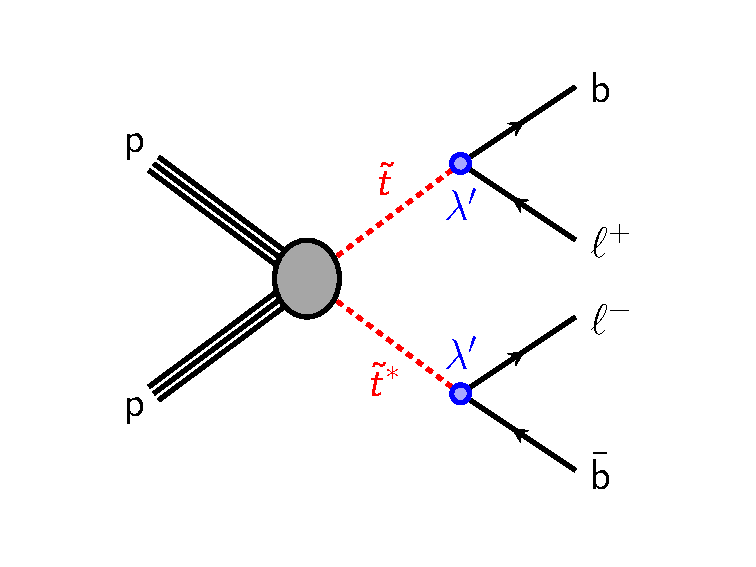
\includegraphics[width=0.60\textwidth]{figs/blstop/b_minus_l_stop_stop.pdf}
  \caption{Simplified model of pair production of stop quarks, with decay to a
    charged lepton and $b$-quark.
  }
  \label{fig:blstop_diagram}
\end{figure}


The experimental signature is two oppositely charged leptons and two identified
$b$-jets.
The analysis considers $eebb$, $e \mu bb$, and $\mu \mu bb$ final states.
Final states with $\tau$ leptons are not considered for this search.
The distinguishing features are two pairs, each of a lepton and a $b$-jet, with
a resonance in the invariant mass distribution of each pair.
In contrast to $R$-parity conserving searches, there is no significant missing
transverse momentum.

Previous searches for lepto-quarks at ATLAS~\cite{ATLAS:2013oea,
ATLAS:2012aq, Aad:2011ch, Aad:2011uv} and
CMS~\cite{Khachatryan:2014ura, CMS:2014qpa, Chatrchyan:2012sv,
Chatrchyan:2012vza} have considered pair production of first, second,
and third generation lepto-quarks, but have not examined the signature
of a resonance in the invariant mass of an electron and a $b$-jet or a
muon and a $b$-jet.  The results of these searches have already been
interpreted to set limits on the stop mass and its decay
branching fractions in the $B-L$
model~\cite{Marshall:2014cwa, Marshall:2014kea}.

Chapter~\ref{ch:theory} gives a description of the Standard Model (SM) of
particle physics and Supersymmetry, a popular extension to the SM.
The concept of $R$-parity, and the $B-L$ extension to the SM is also discussed
in this chapter.
Emphasis is placed on the phenomenology of this model.

The LHC and ATLAS detector, along with the triggering system and event
reconstruction is introduced in Chapter~\ref{ch:lhc}.
Chapter~\ref{ch:trt} describes the Transition Radiation Tracker sub-detector
in more detail.
{\color{red} TODO decide if this chapter actually belongs in the final version}
The Monte Carlo event generator tools used for estimating the detector
response and efficiency to reconstruct the signal process, estimate systematic
uncertainties, and to predict the backgrounds from SM processes, are outlined
in Chapter~\ref{ch:mc}.

Chapter~\ref{ch:bl_stop} describes the stop search.
This chapter reviews the search strategy, event selection, and interpretation
of the results.
The chapter concludes with a brief description of proposed improvements to the
analysis.
{\color{red} TODO decide if this section actually fits in the final version}

%% \chapter[htoc-titlei][hhead-titlei]{htitlei}
%% -----------------------------------------------------------------------------
\chapter[Theoretical overview][Theory]{Theoretical overview}
\label{ch:theory}

{\color{red} I'll need to go back and re-read through some books/papers before
  writing this chapter!}

{\color{red} Evelyn: 
keep this brief by referencing as much as possible.
Certainly contrast assumption of RPC vs assumption of RPV for experimental
searches.
Both are possibilities.
Stop as LSP does give unique (crazy?) signature not well
tested by previous searches (include LQ exclusion plot).
Could have different
decay rates to e, mu, tau.
}

The universe, as we know it, comprises fundamental matter particles, and
four fundamental forces.
These forces include gravity, electromagnetism, and the strong and weak nuclear
forces.
Despite being the weakest of the four forces, gravity is certainly the most
familiar to everyday life, as it assures objects fall to the ground.
The Gravitational force is described by the general theory of relativity, and
to this day, a successful quantum theory of gravity has yet to be developed.
Since gravity is so weak, it does not significantly affect the physics at the
LHC energy scale, and can safely be ignored for the purpose of this thesis.
Of the remaining three forces,  electromagnetism and the weak force have been
shown to come from the same underlying interactions, called the electroweak
force.
The electroweak and strong forces are described by the Standard Model of
Particle Physics.

In this chapter, a brief overview of the theoretical background for this thesis
is presented.
The Standard Model and its shortcomings are discussed
in \cref{sec:sm,sec:sm_shortcomings}.
Supersymmetry, a popular extension to the Standard Model, is introduced in
Section~\ref{sec:susy}.
The chapter concludes with a presentation of the particular $B-L$ extension to
the SM, which is the focus of the search presented in this dissertation.
Section~\ref{sec:theory_bl_extension} includes presents a brief description of
the underlying theory, as well as some of the interesting phenomenology expected
in the scenario where the scalar top is the LSP.

%% ------------------------------------------------------------------------------
\FloatBarrier
\section{Standard Model}
\label{sec:sm}

In this section, the Standard Model (SM) of particle physics is described in
brief.
The SM is a very rich subject, and a more complete description can be found in
References~\cite{Agashe:2014kda,opac-b1131978,halzen1984quarks}.
The SM is a quantum field theory which encapsulates the current understanding
of the elementary particles, and their interactions, and has been developed,
and rigorously tested by experiments over the last fifty years.
In 2012, the final particle predicted by the SM, the ``Higgs boson`` was
discovered at CERN by the ATLAS and CMS collaborations, marking a great
achievement for the both the experimental collaborations and the theorists
who predicted the particle's existence.
The SM Lagrangian is a non-abelian gauge theory with symmetry group 
$\mathrm{SU}(3)_\mathrm{C} \times
\mathrm{SU}(2)_\mathrm{L} \times
\mathrm{U}(1)_\mathrm{Y}$,
which describes the matter content of the universe, as well as the interactions
of the strong and electroweak forces.
The matter content in the SM is made up of fermions (spin \nicefrac{1}{2}),
called quarks and leptons.
Massless gauge bosons (spin 1) mediate the interactions of the electroweak and
strong forces.

\begin{figure}[ht]
  \centering{
    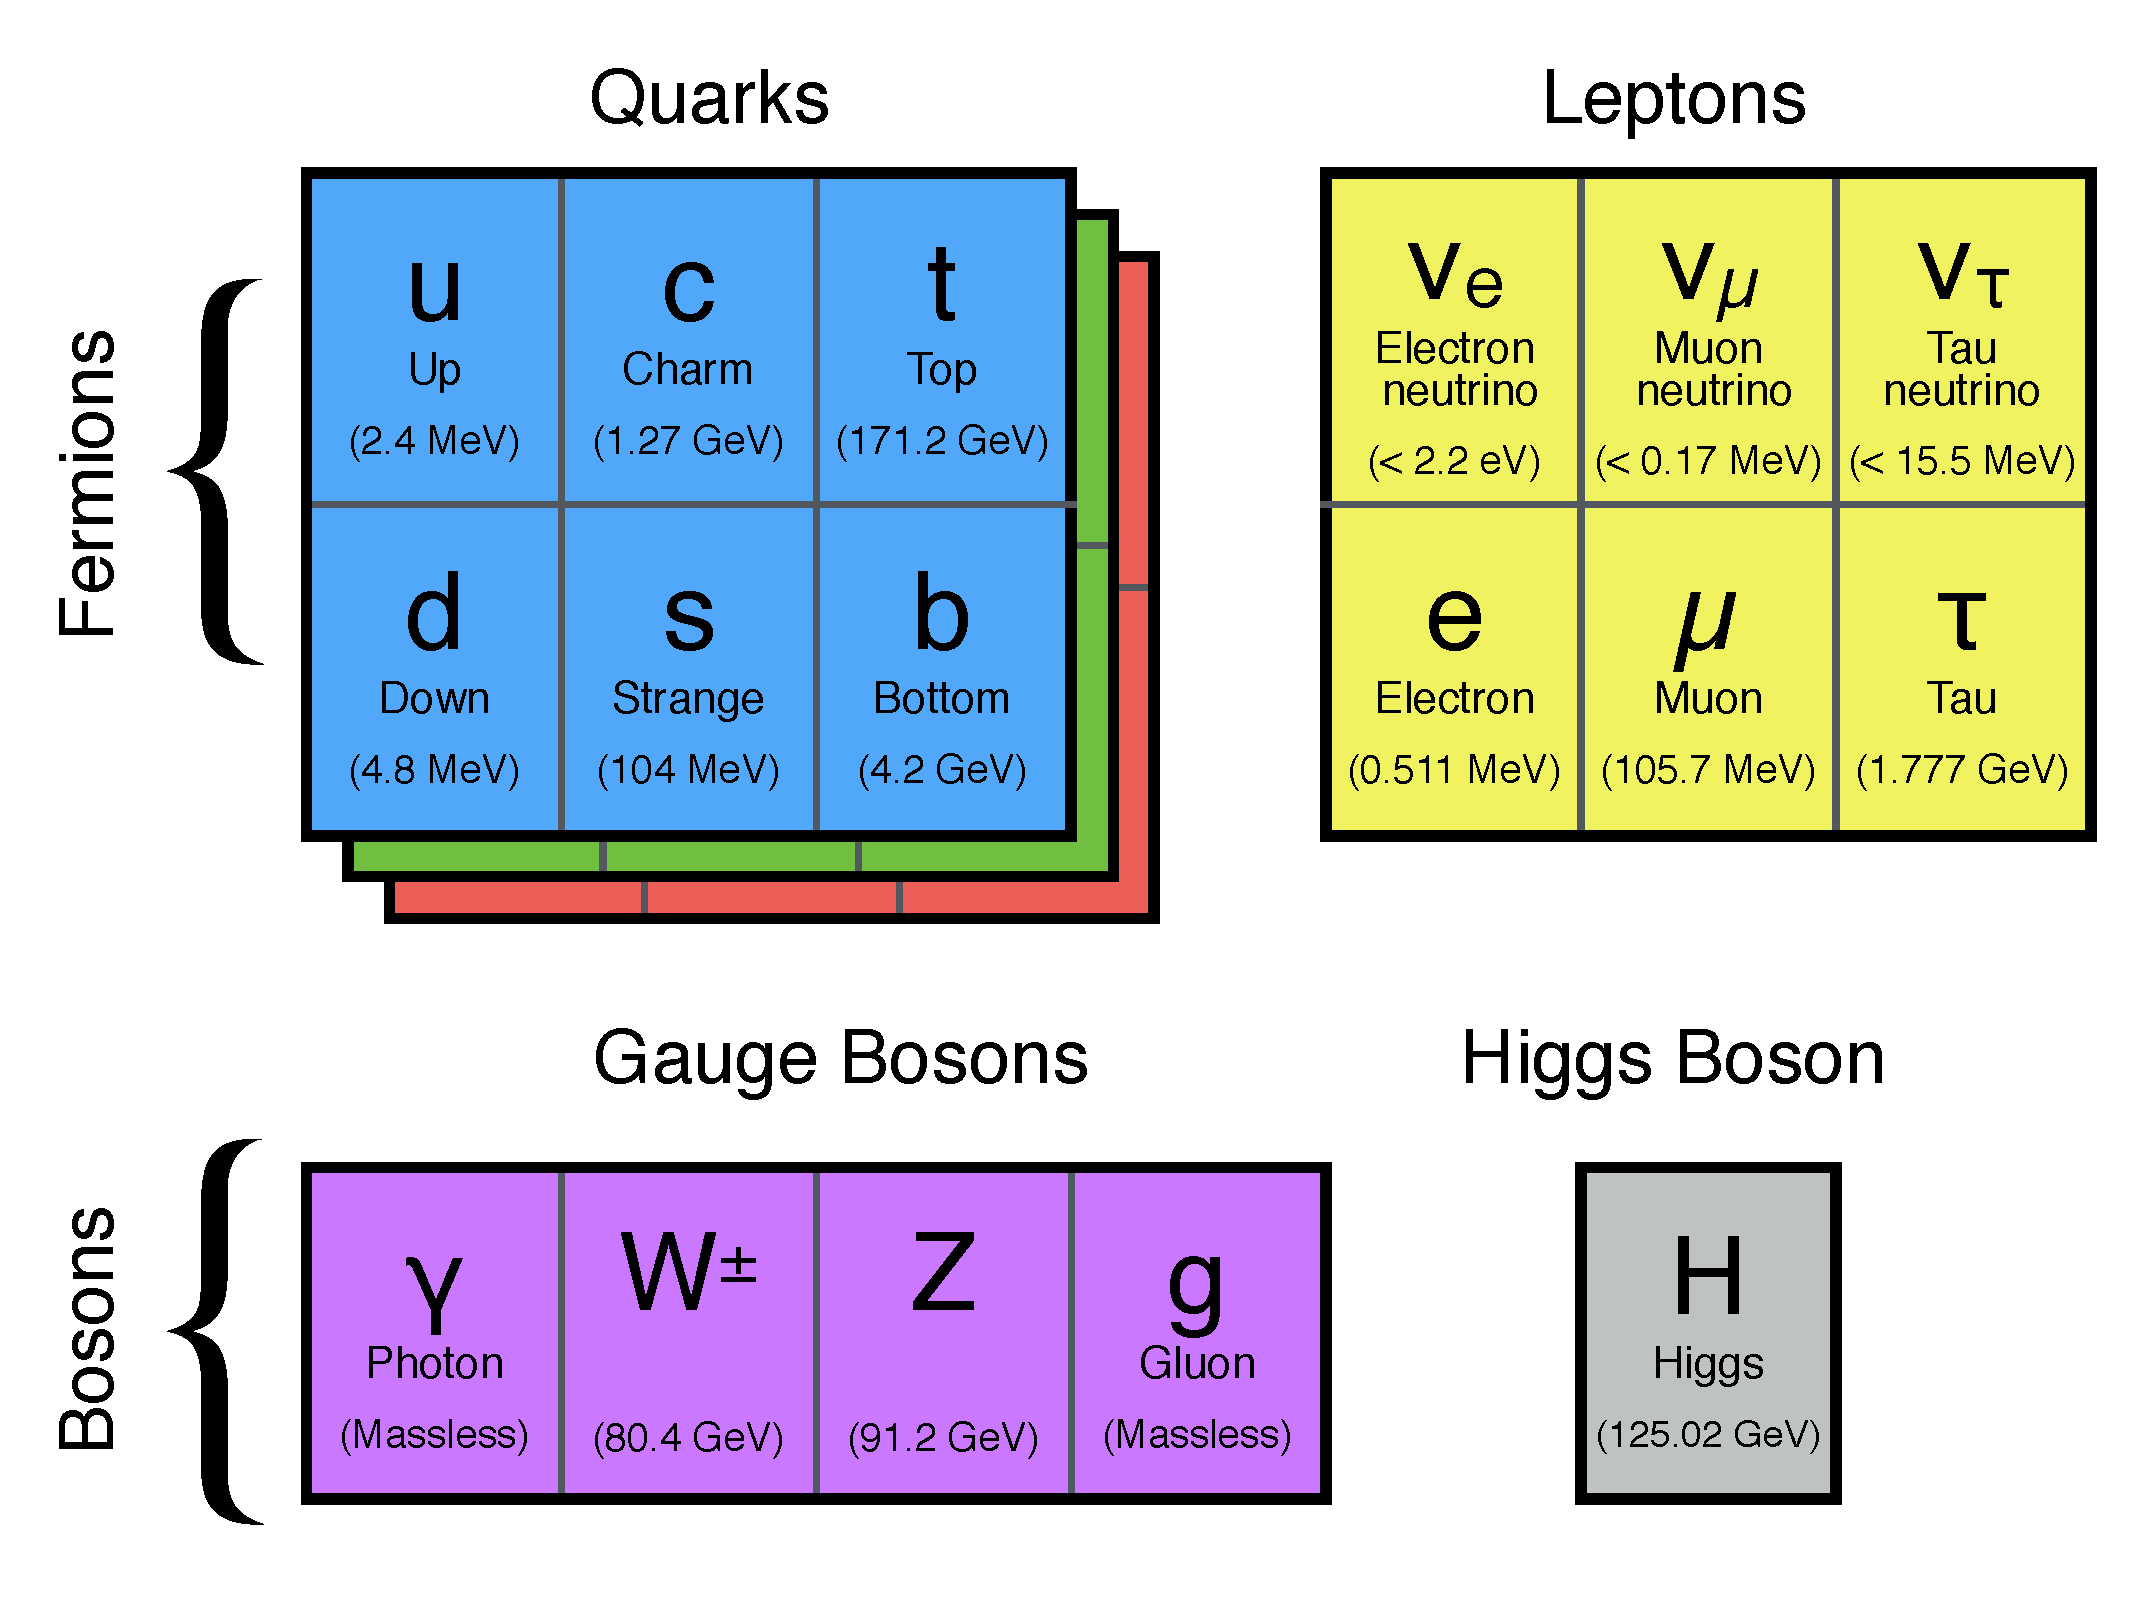
\includegraphics[width=\textwidth]{figs/theory/sm_particle_content.pdf}
    \caption{Fundamental particles described by the Standard Model.
      The masses of each particles are given in parentheses.
    }
    \label{fig:sm_particle_content}
  }
\end{figure}

%% ------------------------------------------------------------------------------
\subsection{Matter}
\label{sec:matter}

The fermionic matter is arranged into three families, or generations, each
containing quarks and leptons.
These particles can be charged under each part of the SM symmetry group,
where the particle's charge determines how it interacts with each of the
corces.
Each generation contains two chiral left-handed quarks, arranged in a isospin
doublet, consisting of an up-type and a down-type quark.
There are also two chiral left-handed leptons, one with electric charge, and
a neutrino, which is electrically neutral.
As with the quarks, the two left-handed leptons are arranged into an isospin
doublet.
Finally, each fermionic family contains chiral right-handed counterparts to
the two quarks, and the charged lepton.
No right-handed neutrinos are included in the SM, as they would no react with
any known forces, as will be explained shortly.
The right-handed fermions are isospin singlets.
The three generations are essentially copies of one another, differing only in
the mass of the constituent particles, and the familiar world is made up
entirely of particles from the first generation.
The reason for exactly three generations, not more or less, remains a mystery.
A summary of the SM matter content, with the charges under the various
parts of the SM symmetry group is shown in Table~\ref{tab:sm_matter_content}.

\begin{table}
  \caption{Summary of the matter particles described by the SM, along with the
    associated quantum numbers.
    The quantum numbers include the spin, electric charge $Q$, the third
    component of weak isospin $T_3$, hypercharge $Y$, and the allowable color
    charges.
  }
  \label{tab:sm_matter_content}
  \begin{center}
    \begin{tabular}{ccccccccc}
      \toprule
      \multirow{2}{*}{Fermions} &
      \multicolumn{3}{c}{Generation} &
      \multirow{2}{*}{Spin} &
      \multirow{2}{*}{$Q$} &
      \multirow{2}{*}{$T_3$} &
      \multirow{2}{*}{$Y$} &
      \multirow{2}{*}{Color}
      \\[1ex]
      & 1 & 2 & 3
      \\
      \midrule
      \addlinespace[1ex]
      %%
      \multirow{5}{*}{Quarks} &
      \multirow{2}{*}{$\left(
        \begin{tabular}{c} u \\ d \end{tabular} \right)_{L}$ } & % (u d) quarks
      \multirow{2}{*}{$\left(
        \begin{tabular}{c} c \\ s \end{tabular} \right)_{L}$ } & % (c s) quarks
      \multirow{2}{*}{$\left(
        \begin{tabular}{c} t \\ b \end{tabular} \right)_{L}$ } & % (t b) quarks
      \multirow{2}{*}{$\frac{1}{2}$} & % Spin
      $+\frac{2}{3}$ & % Q
      $+\frac{1}{2}$ & % T3
      \multirow{2}{*}{$\frac{1}{3}$} & % Y
      \multirow{2}{*}{r, g, b} % color
      \\[1ex]
      %%
      & % Quarks
      & % (u d) quarks
      & % (c s) quarks
      & % (t b) quarks
      & % spin
      $-\frac{1}{3}$ & % Q
      $-\frac{1}{2}$ & % T3
      & % Y
      % color
      \\
      %%
      \cmidrule{2-9}
      %%
      &
      $u_R$ &
      $c_R$ &
      $t_R$ &
      $\frac{1}{2}$ & % spin
      $+\frac{2}{3}$ & % Q
      0 & % T3
      $+\frac{4}{3}$ & % Y
      r, g, b % color
      \\[1ex]
      %%
      &
      $d_R$ &
      $s_R$ &
      $b_R$ &
      $\frac{1}{2}$ & % spin
      $-\frac{1}{3}$ & % Q
      0 & % T3
      $-\frac{2}{3}$ & % Y
      r, g, b % color
      \\
      %%
      \midrule
      %%
      \multirow{3}{*}{Leptons} &
      \multirow{2}{*}{$\left(
          \begin{tabular}{c} $\nu_{e}$ \\ e \end{tabular}
        \right)_{L}$ } &
      \multirow{2}{*}{$\left(
          \begin{tabular}{c} $\nu_{\mu}$ \\ $\mu$ \end{tabular}
        \right)_{L}$ } &
      \multirow{2}{*}{$\left(
          \begin{tabular}{c} $\nu_{\tau}$ \\ $\tau$ \end{tabular}
        \right)_{L}$ } &
      \multirow{2}{*}{$\frac{1}{2}$} & % spin
      0 & % Q
      $+\frac{1}{2}$ & % T3
      \multirow{2}{*}{-1} & % Y
      \multirow{2}{*}{-} % color
      \\[1ex]
      %%
      & % Leptons
      & % (nue e)
      & % (numu mu)
      & % (nutau mu)
      & % spin
      $-1$ & % Q
      $-\frac{1}{2}$ & % T3
      & % Y
      % color
      \\
      \cmidrule{2-9}
      %%
      & % Leptons
      $e_{R}$ &
      $\mu_{R}$ &
      $\tau_{R}$ &
      $\frac{1}{2}$ & % spin
      $-1$ & % Q
      0 & % T3
      $-2$ & % Y
      - % color
      \\
      \bottomrule
    \end{tabular}
  \end{center}
\end{table}

%% ------------------------------------------------------------------------------
\subsection{Quantum electrodynamics}
\label{sec:qed}

In addition to a charge, each piece of the SM symmetry group is associated with
a massless gauge boson, which mediates the interactions between particles.
The electroweak sector has the symmetry group
$\mathrm{SU}(2)_\mathrm{L} \times \mathrm{U}(1)_\mathrm{Y}$, and describes the
interactions with fields with isospin or hypercharge ($Y$) in a theory called
quantum electrodynamics (QED).
The electroweak sector is a chiral theory, meaning right- and left-handed
particles transform differently under the gauge group.
Left-handed fermions have a value of the third component of isospin equal to
$\pm \nicefrac{1}{2}$, while right-handed particles have no isospin, and do
not interact with the weak force.
The gauge bosons associated with the electroweak sector are three $W^{i}$
bosons, arranged in a weak isospin triplet, and a $B^0$ boson, which is a weak
isospin singlet.

Since chiral fields translate differently, depending on their chiral handedness,
there can be no mixing between the right- and left-handed states, which would
break gauge invariance.
Unfortunately, a mass term, allows for exactly this mixing, implying the
fermions, as well as the gauge bosons must be massless.
On the other hand, the weak force is observed to be short ranged, implying
massive gauge bosons, and fermions do indeed have measurable masses.
Adding masses to a chiral quantum field theory is a difficult endeavor, and
is achieved through a process called ``spontaneous symmetry breaking,'' which
is explained in Section~\ref{sec:higgs}.
The broken symmetry leads to a mixing of the $W^3$ and $B^0$ gauge bosons into
a massless photon, and the massive $Z$ boson.
The $W^1$ and $W^2$ become the massive $W^{+}$ and $W^{-}$.
The $W^{\pm}$ and $Z$ bosons both have mass, and act as the propagator of the
weak force, while the massless photon mediates the electromagnetic force.

Since right-handed neutrinos have no charge under any part of the SM symmetry
group, they are not expected to interact with the known components of the SM,
and are therefore not included as part of the theory.
There are extensions to the SM, however, which do include right-handed
neutrinos, including the one described in Section~\ref{sec:theory_bl_extension}.

%% ------------------------------------------------------------------------------
\subsection{Quantum chromodynamics}
\label{sec:qcd}

The $\mathrm{SU}(3)_\mathrm{C}$ part of the SM Lagrangian corresponds to the
strong force, with a corresponding ``color'' charge, and is described by the
theory of quantum chromodynamics (QCD).
Quarks are colored objects, having red, green, or blue charge, while leptons
have no color charge, and thus do not interact directly with the strong
force.
The eight massless gauge bosons associated with the
$\mathrm{SU}(3)_\mathrm{C}$ symmetry group are called gluons, and are
themselves colored objects.
This leads to self interaction, and some interesting phenomenology!

Because the gluon are allowed to interact with one another, QED and QCD have
some very important differences.
Perhaps, the most interesting, is related to the concept of ``screening''.
In QED, as one moves further from a charged paricle, the charge tends to look
smaller as a result of the polarization of the vacuum around the charge, where
electron pairs pop out of the vacuum.
The further from the particle one is, the more electron pairs are visible,
obscuring the initial charge more.
In QCD, this same screening effect occurs, with quark-anti-quark pairs being
pair-produced from the vacuum, however gluon pairs may also be produced out of
the vacuum.
These gluon pairs produce the opposite screening effect, known as
``anti-screening,'' increasing the effective charge observed.
Rather than charges being screened, as in QED, there is a net anti-screening
effect for objects with color charge.

As two colored particles get very close together, the anti-screening is very
small, and they can be treated as free particles, in an effect known as
``asymptotic freedom.''
Alternatively, as two charged particles move apart, the polarization of the
vacuum between them results in an increasing energy buildup, until it is
energetically favorable to pair produce a quark-anti-quark pair from the vacuum.
For this reason, no free quarks or gluons have been observed, rather any
objects with color charge will tend to into bound states called ``hadrons,''
which has no net color.
Hadrons can either be a bound state of a quark-anti-quark pair, called mesons,
or three-quark bound states, called baryons.
The anti-quark contained in a meson must have the corresponding anti-color of 
the constituent quark.
Similarly, the three quarks, which make up a baryon, must have colors that add
to ``white,'' meaning one red , one green, and one blue quark.

In particle collisions, this effect also leads to the phenomenon of ``jets,''
where a spray of hadrons is projected at the particle detector, resulting from
the multiple colored objects being pulled apart due to the energy of the
collision.

%% - - - - - - - - - - - - - - - - - - - - - - - - - - - - - - - - - - - - - - -
\FloatBarrier
\subsection{Brout-Englert-Higgs mechanism}
\label{sec:higgs}

As mentioned in Section~\ref{sec:qed}, the fermions and gauge bosons described
in the SM Lagrangian are massless, however, many of those observed in nature
do, in fact, have a non-negligible mass.
This would seem to allow for the mixing of chiral left- and right-handed
fields, which would in turn break gauge invariance.
A method to add mass terms to the SM Lagrangian without breaking the necessary
gauge invariance was developed during the 1960's by several groups of theorists,
including Robert Brout and Francois Englert~\cite{PhysRevLett.13.321},
Peter Higgs~\cite{Higgs1964132,PhysRevLett.13.508},
and Gerald Guralnik, Carl R. Hagen, and Tom Kibble~\cite{PhysRevLett.13.585}
working in parallel, and is commonly called the Brout-Englert-Higgs (BEH)
mechanism.
The BEH mechanism adds an additional complex scaler field to the Lagrangian,
which acquires a vacuum expectation value (vev), which ``spontaneously''
breaks the symmetry of the SM Lagrangian.

Each spontaneously broken symmetry leads to new massive scalar particle, know
as a ``Goldstone boson.''
The gauge bosons can then absorb these Goldstone bosons in a process where they
acquire a mass.
Recall, before symmetry breaking, the electroweak sector has four massless
gauge bosons, the $W^1$, $W^2$,  $W^3$, and the $B^0$, however experiments
observe massive $W^{\pm}$, and the $Z$ bosons, associated with the weak force,
and a massless photon to mediate the electromagnetic force.
An electric charge $Q$ is also conserved.
This implies that the
$\mathrm{SU}(2)_\mathrm{L} \times \mathrm{U}(1)_\mathrm{Y}$ of QED is broken in
a way that leaves only a $\mathrm{U}(1)_\mathrm{EM}$ symmetry group.
This symmetry breaking requires at least three Goldstone bosons to be absorbed,
and give masses to the gauge bosons.
The simplest method to accomplish this is to add a complex scalar field
\begin{equation}
  \Phi = \begin{pmatrix} \phi^+ \\ \phi^0 \end{pmatrix},
    \label{eqn:scalar_field}
\end{equation}
%which is a doublet with positive hypercharge ($Y=\nicefrac{1}{2}$).
which is a doublet with positive hypercharge ($Y=1$).

To show how this, it is useful to consider the SM Lagrangian, ignoring the
QCD part,
\begin{equation}
  \mathcal{L} =
  - \frac{1}{4} W_{\mu\nu}^{a} W_{a}^{\mu\nu}
  - \frac{1}{4} B_{\mu\nu} B^{\mu\nu}
  + \bar{L}_i \left(i D_{\mu} \gamma^{\mu} \right) L_i
  + \bar{e}_{\mathrm{R},i}\left(i D_{\mu} \gamma^{\mu}\right)e_{\mathrm{R},i},
\end{equation}
where the $i$ index runs over the three generations, the $\mu$,$\nu$ are
Lorentz indices, and $a$ runs over the generators in the gauge group.
The field strengths are given by
\begin{eqnarray}
  W_{\mu\nu}^{a} & = &
  \partial_{\mu}W_{\nu}^{a} - 
  \partial_{\nu}W_{\mu}^{a} +
  g_{2}\epsilon^{abc}W_{\mu}^{b}W_{\nu}^{c}
  \\
  B_{\mu\nu} & = &
  \partial_{\mu}B_{\nu} - 
  \partial_{\nu}B_{\mu},
\end{eqnarray}
and the covariant derivatives for the left- and right-handed lepton fields are
\begin{eqnarray}
  D_{\mu}L_\mathrm{L} & = &
  \left(
    \partial_{\mu} - ig_{2}T_{a}W_{\mu}^{a} - ig_{1}YB_{\mu}
  \right) L_\mathrm{L}
  \\
  D_{\mu}e_\mathrm{R} & = &
  \left(
    \partial_{\mu} - ig_{1}YB_{\mu}
  \right) e_\mathrm{R}.
\end{eqnarray}
$T_a$ are the generators of the gauge group, and $g_1$ and $g_2$ are the
coupling constants for electroweak interactions.

Adding the complex scalar field from Equation~\ref{eqn:scalar_field} adds an
additional scalar part to the Lagrangian,
\begin{equation}
  \mathcal{L} =
  \left(D^{\mu}\Phi\right)^{\dagger}\left(D_{\mu}\Phi\right) - V(\Phi),
  \label{eqn:scalar_lagrangian}
\end{equation}
where the first term is the kinetic term, and $V(\Phi)$ is the scalar
potential.
The exact form of the scalar potential is not known, however, the simplest
possible form that has the desired properties can be used
\begin{equation}
  V(\Phi) = \mu^2 \Phi^{\dagger}\Phi + \lambda\left(\Phi^{\dagger}\Phi\right)^2.
\end{equation}
This form is an assumption that provides the required spontaneous symmetry
breaking, while remaining renormalizable.
In order for the vacuum to be stable, $\lambda$ must be positive.
The choice of the $\mu^2$ parameter affects the shape of the scalar potential,
as shown in Figure~\ref{fig:symmetry_breaking}.
In the configuration with $\mu^2 > 0$, the scalar potential is always positive,
and the minimum occurs at
\begin{equation}
  \bra{0} \Phi \ket{0} = \begin{pmatrix} 0 \\ 0 \end{pmatrix}.
\end{equation}
There is no spontaneous symmetry is this scenario.
On the other hand, if $\mu^2 < 0$, the scalar potential takes on the famous
``Mexican hat'' shape, and the minimum of the potential is no longer located at
the origin.
With the minimum of the scalar potential located away from the origin, the
neutral part of the scalar field acquires a vacuum expectation value (vev) $v$,
\begin{equation}
  \bra{0} \Phi \ket{0} =
  \Phi_0 =
  \frac{1}{\sqrt{2}} \begin{pmatrix} 0 \\ v \end{pmatrix},
  v = \sqrt{\frac{-\mu^2}{\lambda}}.
\end{equation}
By acquiring a vev, electroweak symmetry is spontaneously broken.

\begin{figure}[ht]
  \centering
  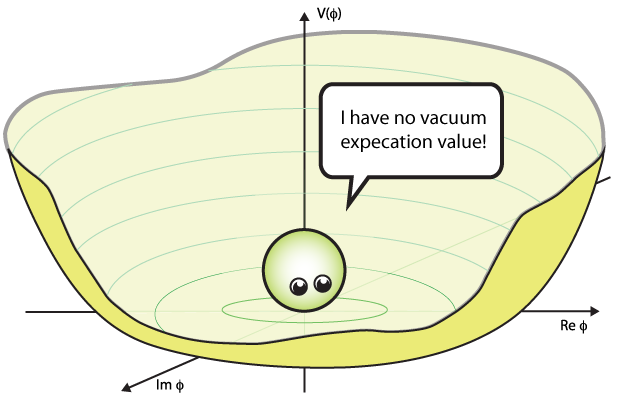
\includegraphics[width=0.48\textwidth]
      {figs/theory/BoringPotential.png}
  \\
  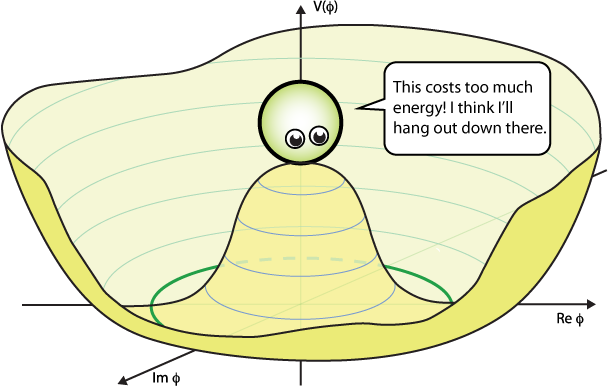
\includegraphics[width=0.48\textwidth]
      {figs/theory/Higgs-Potential-lookdown.png}
  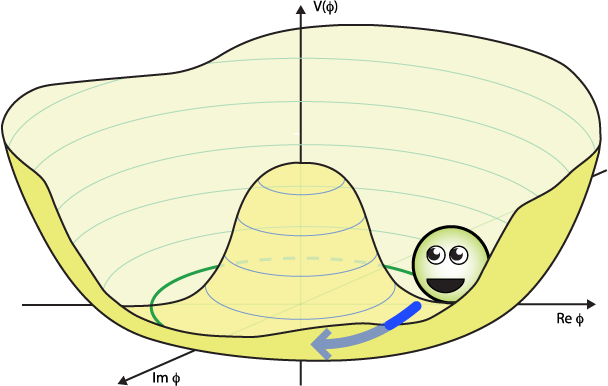
\includegraphics[width=0.48\textwidth]
      {figs/theory/Higgs-Potential-Goldstone.png}
      \caption{The scalar potential under two configurations.
        The configuration on the top shows the case where $\mu^2 > 0$, where
        the scalar potential is always positive.
        In this configuration, the scalar potential has a minimum at the origin.
        The configuration with $\mu^2 < 0$ is shown on the bottom.
        In this case, the minimum of the scalar potential occurs away from the
        origin.
        In this scenario, the scalar field moves away from the origin, in a
        process of spontaneous symmetry breaking.
        The green line corresponds to the circle of minimum potential,
        corresponding to the massless Goldstone
      mode~\cite{QuantumDiariesHiggs}}.
  \label{fig:symmetry_breaking}
\end{figure}

Since the charged part of the scalar field does not acquire a vev,
electromagnetism is not broken, leaving a remaining $U(1)_\mathrm{EM}$
symmetry with a conserved charge of
\begin{equation}
  Q = T_3 + \frac{Y}{2},
\end{equation}
corresponding to the electric charge.

Expanding the scalar field $\Phi$ around it's minimum $\Phi_0$, one gets
\begin{equation}
  \Phi(x) = \frac{1}{\sqrt{2}} \begin{pmatrix} 0 \\ v + h(x) \end{pmatrix},
\end{equation}
with $h(x)$ being a new scalar field.
Inserting this into the kinetic term of Equation~\ref{eqn:scalar_lagrangian},
and redefining the gauge fields as
\begin{eqnarray}
  W_{\mu}^{\pm} & = & \frac{1}{\sqrt{2}}
                      \left( W_{\mu}^{1} \mp W_{\mu}^{2} \right),
  \\
  Z_{\mu} & = & \frac{1}{\sqrt{g_1^2 + g_2^2}}
                \left( g_2 W_{\mu}^{3} - g_1 B_{\mu} \right),
  \\
  A_{\mu} & = & \frac{1}{\sqrt{g_1^2 + g_2^2}}
                \left( g_2 W_{\mu}^{3} + g_1 B_{\mu} \right),
\end{eqnarray}
where the redefined gauge fields correspond to the physical gauge bosons
of QED, the $W^{\pm}$, $Z$, and the photon.
The covariant derivative becomes
\begin{equation}
  \left| D_{\mu}\Phi \right|^2 =
  \frac{1}{2} \left( \partial_{\mu} H \right)^2 +
  \frac{1}{2} g_{2}^{2} \left(v + H\right)^2 W_{\mu}^{+}W^{\mu -} +
  \frac{1}{8} \left(v + H\right)^2 \left(g_{1}^{2} + g_{2}^{2} \right)
    Z_{\mu}Z^{\mu}.
\end{equation}
It can be seen that the gauge bosons take on the following masses through their
interactions with the scalar field
\begin{eqnarray}
  M_{W} &=& \frac{1}{2} v g_2 \\
  M_{Z} &=& \frac{1}{2} v \sqrt{g_1^2 + g_2^2} \\
  M_{A} &=& 0
\end{eqnarray}
It is important to note that there is no term for the photon, implying it does
not interact with the scalar field, and therefore, does not pick up a mass
term.
Three of the degrees of freedom from the scalar field that would be Goldstone
bosons have been absorbed by the gauge bosons, giving them mass.
There is one remaining degree of freedom, which becomes the Higgs boson.
The Higgs boson itself has mass, equal to
\begin{eqnarray}
  m_H &=& 2 \lambda v^2 \\
      &=& 2\mu^2.
\end{eqnarray}
This mass corresponds to the remaining degree of freedom in the scalar
potential, where the field can oscillate in the radial direction, as shown in
Figure~\ref{fig:higgs_mass}.
The Higgs mass has no other handles in the SM, and must be determined
experimentally.
It was found to be equal to
$125.02^{+0.22}_{0.27}\mathrm{(stat)}^{+0.14}_{-0.15}\mathrm{(syst)} \GeV$
by the ATLAS and CMS experiments.

\begin{figure}[ht]
  \centering
  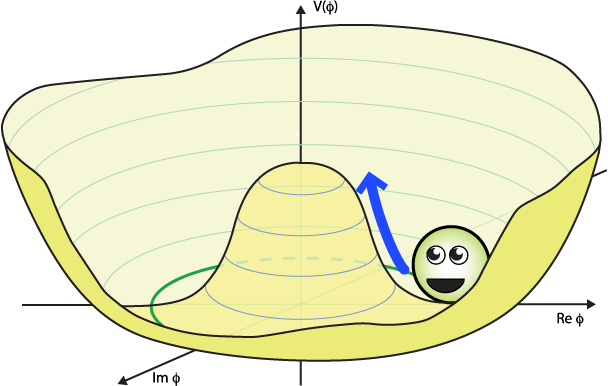
\includegraphics[width=0.48\textwidth]{figs/theory/Higgs-Potential-radial.png}
  \caption{The Higgs boson corresponds to an excitation in the radial direction
    of the scalar potential~\cite{QuantumDiariesHiggs}.
  }
  \label{fig:higgs_mass}
\end{figure}

The final piece to add to the SM are masses for the fermions, which are
introduced through Yukawa cuplings between the fermion fields and the scalar
field.
An additional set of terms are added to the Lagrangian for the interactions
between the scalar field and the fermion sector.
The portion that represents the first generation of fermions is
\begin{equation}
  \mathcal{L}_\mathrm{F} =
  - G_e \bar{L} \Phi e_\mathrm{R}
  - G_d \bar{Q} \Phi d_\mathrm{R}
  - G_u \bar{Q} \tilde{\Phi} u_\mathrm{R}
  + \mathrm{h.c.}.
  \label{eqn:fermion_lagrangian}
\end{equation}
There are copies of these terms for the second and third generations of
fermions.
A new term, $\tilde{\Phi}$ was introduced, which is the conjugate of $\Phi$
with negative hypercharge ($Y = 1$), and is equal to
\begin{eqnarray}
  \tilde{\Phi} &=& i \tau_2 \Phi^{*} \\
               &=& \frac{1}{\sqrt{2}} \begin{pmatrix} v + h \\ 0 \end{pmatrix}.
\end{eqnarray}
Substituting terms into Equation~\ref{eqn:fermion_lagrangian} gives
\begin{align}
  \begin{split}
    \mathcal{L}_\mathrm{F} =
      - \frac{1}{\sqrt{2}}
      &
      \left[
      G_e
    \begin{pmatrix} \bar{\nu} & \bar{e} \end{pmatrix}_\mathrm{L}
    \begin{pmatrix} 0 \\ v+h \end{pmatrix}
      e_\mathrm{R}
      %% 
      + G_d
    \begin{pmatrix} \bar{u} & \bar{d} \end{pmatrix}_\mathrm{L}
    \begin{pmatrix} 0 \\ v+h \end{pmatrix}
      d_\mathrm{R}
      \right.
      \\
      &
      \left.
      %%
      + G_u
    \begin{pmatrix} \bar{u} & \bar{d} \end{pmatrix}_\mathrm{L}
    \begin{pmatrix} v+h \\ 0 \end{pmatrix}
      u_\mathrm{R}
    \right]
    %%
    + \mathrm{h.c.}
    %%
  \end{split}
\end{align}
%%
\begin{equation}
  \mathcal{L}_\mathrm{F} =
  - \frac{1}{\sqrt{2}}
  (v+h)
  \left(
    G_e \bar{e}_\mathrm{L} e_\mathrm{R} +
    G_d \bar{d}_\mathrm{L} d_\mathrm{R} +
    G_u \bar{u}_\mathrm{L} u_\mathrm{R}
  \right) + \mathrm{h.c.}.
  \label{eqn:expanded_fermion_lagrangian}
\end{equation}

Generic fermion mass terms are of the form
$m \bar{f}_\mathrm{L} f_\mathrm{R} + \mathrm{h.c.}$, so reading
Equation~\ref{eqn:expanded_fermion_lagrangian}, one can see the fermion masses
are
% \begin{align}
%   \begin{split}
%     m_e = & \frac{G_e v}{\sqrt{2}} \\
%     m_u = & \frac{G_u v}{\sqrt{2}} \\
%     m_d = & \frac{G_d v}{\sqrt{2}}.
%   \end{split}
% \end{align}
\begin{equation}
    m_e = \frac{G_e v}{\sqrt{2}},~~~~~
    m_u = \frac{G_u v}{\sqrt{2}},~~~~~
    m_d = \frac{G_d v}{\sqrt{2}}.
\end{equation}
The $h$ is dropped because it is the remnant of the Higgs doublet, and expected
to be negligible.
There are of course similar mass terms for the second and third generation
fermions.
Since the neutrinos have no isospin, they do not interact with the scalar
potential, and therefore, do not pick up a mass.
It should also be noted that the $G$'s, thus the fermion masses, are not
predicted by the SM, and the fermion masses must be measured, and inputed
into the theory.

%% -----------------------------------------------------------------------------
\FloatBarrier
\section{Shortcomings}
\label{sec:sm_shortcomings}

While the SM has been a very successful theory in describing particles
and their interactions across many orders of magnitude, it does have some
shortcomings.
Some of these shortcomings, such as the existence of dark matter arise from
experimental observations, which point toward potential problems with the SM,
and currently constructed.
Others, such as the Hierarchy problem arise from parts of the SM, which seem
to require, seemingly unnatural, amounts of ``fine tuning'' of the parameters
of the theory.

%% -----------------------------------------------------------------------------
\FloatBarrier
\subsection{Gravity}

One (seemingly obvious) feature, missing from the SM is the gravitational
force.
This seems counterintuitive because this is probably the force people are most
familiar with, in their daily lives.
However, gravity remains a very weak force, compared to the electroweak scale,
and no successful quantum theory of gravity has been created.
A spin 2 graviton particle has been proposed, which seems as if it can be added
to the SM, but experiments have yet to observe such a particle.

%% -----------------------------------------------------------------------------
\FloatBarrier
\subsection{Dark matter and dark energy}

Cosmological experiments over the past several
decades\cite{Clowe:2006eq,Ade:2013zuv} have shown that observable matter
only makes up 5\% of the observable universe.
It is still unknown what makes up the remaining 95\%!
The unknown component is generally broken up into two categories, based on
their expected properties.
Dark matter is localized, and tends to be found in clumps, while dark energy
permeates all of space.

From the perspective of gravity, dark matter is expected to behave similar to
normal matter, in that gravity exerts an attractive force on the dark matter.
Dark matter differs in that it does not interact with electromagnetism,
which is why it is called ``dark.''
The other properties of dark matter are unknown.
It is possible that it interacts with the strong or weak forces, however, this
is by no means guaranteed.

Dark energy, on the other hand, opposed the force of gravity, applying a
repulsive force, accelerating the expansion of the universe.

%% -----------------------------------------------------------------------------
\FloatBarrier
\subsection{Neutrino masses}

As shown in Section~\ref{sec:higgs}, the BEH mechanism leaves the neutrinos
massless in the SM because they have no chiral right-handed counterpart, and
don't generate the Yukawa coupling with the scalar field.
Neutrino experiments, have observed neutrino flavor oscillation, suggesting
they do, in fact, have a mass~\cite{PhysRevD.86.010001}.
For these oscillations to occur, the physical neutrino eigenstates must be
a mixture of the flavor eigenstates, and have distinct masses.
This provides evidence that there is a non-zero mass for at least two of the
three neutrino masses.
Some of the proposed mechanisms to generate massive neutrino masses with the
SM are the addition of ``sterile'' right-handed neutrinos, or the possibility
that neutrinos are Majorana particles, and they are their own anti-particle.

%% -----------------------------------------------------------------------------
\FloatBarrier
\subsection{Hierarchy problem}

Several potential problems arises from the large differences in energy scale
between the electroweak scale ($\mathcal{O}(100) GeV$), where experiments are
able to effectively probe, and the Planck scale ($\mathcal{O}(10^{18}) GeV$),
where the effects of gravity can no longer be ignored, and the theory is no
longer valid as it stands.
Because the scales are so different, the bare parameters of the theory can
differ from their renormalized values, or other values in the theory,
by several orders of magnitude.
These problems are classified as ``hierarchy problems,'' and do not immediately
lead to contradictions, as the theory can remain consistent with these large
differences.
However, in order to construct a consistent theory, one is required to accept
a certain amount of ``fine tuning,'' that many find unsatisfying.

A particularly famous hierarchy problem is associated with the mass of the
Higgs boson.
Observed particles masses are a combination of the ``bare'' mass (tree level)
and radiative corrections from additional loop diagrams.
These loop momenta are cut off at the Planck scale, which leaves a lot of room
for the these radiative corrections to increase.
Fermion and gauge boson masses are protected from this high cutoff scale.
Fermions are protected through chiral symmetry, and are only logarithmically
dependent on the cutoff scale. 
Gauge bosons are similarly protected through the local gauge symmetry.
The Higgs boson is a scalar, and has a quadratic dependence on the cutoff
scale.
This tends to push the mass much higher than the weak scale.

The Higgs mass is observed to be at 125~\GeV, so if the bare mass and the
radiative correction terms are truly at such a high scale, it would be a large
coincidence if they simply happen to cancel so precisely.
While it is not impossible, it is extremely unlikely this would happen.
This is the essence of the fine tuning problem.

A way to remove the quadratic dependence on the Planck scale is to introduce
new particles, which have the opposite loop behavior to their SM counterparts.
This is the basic idea of supersymmetry, which is discussed in
Section~\ref{sec:susy}.

%% -----------------------------------------------------------------------------
\FloatBarrier
\section{Supersymmetry}
\label{sec:susy}

Lightest supersymmetric particle (LSP) 

%% - - - - - - - - - - - - - - - - - - - - - - - - - - - - - - - - - - - - - - -
\subsection{R-Parity}
\label{sec:r_parity}

The extension of the Standard Model of particle physics with
supersymmetry (SUSY)~\cite{Miyazawa:1966,Ramond:1971gb,Golfand:1971iw,
Neveu:1971rx,Neveu:1971iv,Gervais:1971ji,Volkov:1973ix,Wess:1973kz,Wess:1974tw}
immediately leads to processes that violate both baryon number ($B$) and
lepton number ($L$), leading to rapid proton decay and
lepton-number-violating processes, such as unseen decays of
$\mu \to e\gamma$, in conflict with experimental bounds.
A conventional assumption to prevent these processes is to impose
conservation of $R$-parity~\cite{Fayet:1976et,Fayet:1977yc,Farrar:1978xj,
Fayet:1979sa,Dimopoulos:1981zb},
defined as $R=(-1)^{3(B-L)+2s}$ where $s$ is the spin of the particle.
This has a value of $+1$ for Standard Model particles and $-1$ for
SUSY particles.
In this case SUSY particles are produced in pairs, and the LSP is stable.
Further, this stable LSP cannot carry electric charge or color charge without
coming into conflict with astrophysical data.
At the LHC, the conventional experimental signature for SUSY particles
includes significant missing transverse momentum due to the non-interaction of
the LSP with the detector.

%% -----------------------------------------------------------------------------
\FloatBarrier
\section{B-L extension}
\label{sec:theory_bl_extension}


%% - - - - - - - - - - - - - - - - - - - - - - - - - - - - - - - - - - - - - - -
\FloatBarrier
\subsection{Motivation}

{\color{red} Why this model? :-) Talk about things like:
\begin{itemize}
\item RPC is overkill to prevent proton decay
\item Links neutrino sector to susy properties
\end{itemize}
}

An alternative approach is to add a local symmetry $\mathrm{U}(1)_{B-L}$ to the
$\mathrm{SU}(3)_\mathrm{C} \times
\mathrm{SU}(2)_\mathrm{L} \times
\mathrm{U}(1)_\mathrm{Y}$ Standard Model with right-handed neutrinos.
The minimal supersymmetric extension then only needs a vacuum expectation value
for a right-handed sneutrino in order to spontaneously break the
$B-L$ symmetry~\cite{FileviezPerez:2008sx, Barger:2008wn, FileviezPerez:2009gr,
Everett:2009vy, Evans:1986ada, Lukas:1998yy, Braun:2005ux, Braun:2005nv,
Braun:2006ae, Ambroso:2009jd, Ambroso:2010pe, Ovrut:2012wg}.
This minimal $B-L$ model violates lepton number but not baryon number, and is
consistent with proton stability and the bounds on lepton number violation.
The LSP can now decay via $R$-parity-violating (RPV) processes, and may now
carry color and electric charge.

%% - - - - - - - - - - - - - - - - - - - - - - - - - - - - - - - - - - - - - - -
\FloatBarrier
\subsection{Phenomenology}

This leads to unique signatures~\cite{FileviezPerez:2012mj, Perez:2013kla,
Ovrut:2012wg, Ovrut:2014rba, Ovrut:2015uea} that are disallowed in conventional
models with $R$-parity conservation.
The case where the LSP is a scalar top (stop) is most interesting
since, in general, the large mass of the top quark acts to make the
lightest stop significantly lighter than the other squarks due to
renormalization group effects~\cite{Barbieri:1987fn,deCarlos:1993yy}.
The stop decays via an RPV interaction to a charged lepton (of any
flavor) and a $b$-quark.
The decay branching fractions to $e b$, $\mu b$, and $\tau b$ may be different,
in a manner related to the neutrino mass
hierarchy seen in Figure~\ref{fig:pheno_bounds}.
Each point in this plot represents a simulation with a particular choice of
model parameters, all varied within a natural range of values, shown in
Table~\ref{tab:pheno_ranges}, and the four colors represent different choices
for the neutrino mass hierarchy and 
$\sin^2\theta_{23}$~\cite{Marshall:2014cwa,Marshall:2014kea}.
There is a clear relation between the neutrino mass hierarchy and the allowed
stop branching ratios, therefore if a stop consistent with this model is
discovered, its properties could potentially give information about the
structure of the neutrino sector.

\begin{figure}[p]
  \centering{
    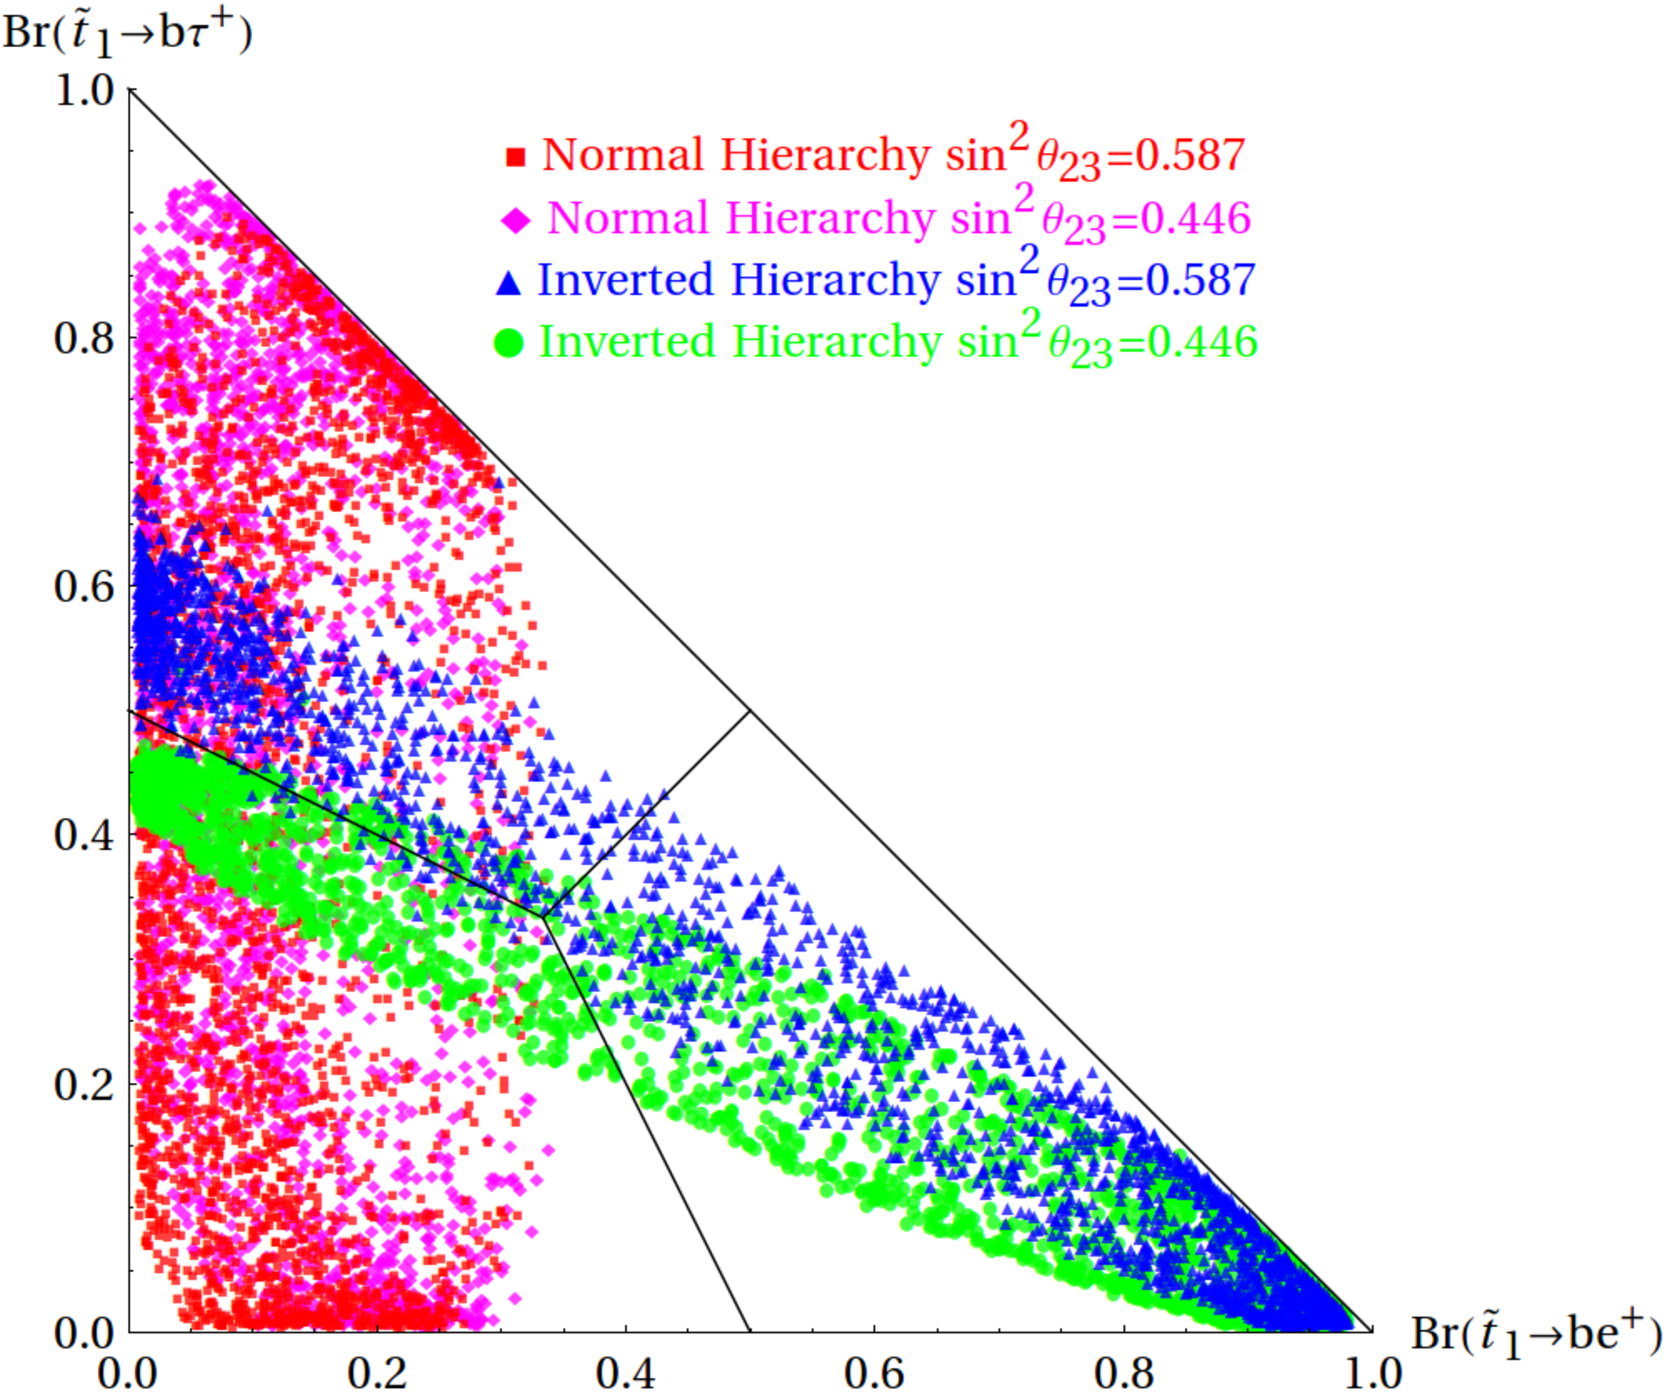
\includegraphics[width=\textwidth]{figs/theory/WithGaussian.pdf}
    \caption{This plot shows the allowed branching ratios for the stop LSP
      for various choices of the neutrino mass hierarchy and
      $\sin^2\theta_{23}$,
      obtained by varying various model parameters within a range of natural
      values shown in Table~\ref{tab:pheno_ranges}~\cite{Marshall:2014cwa}.
    }
    \label{fig:pheno_bounds}
  }
\end{figure}

\begin{table}[ht]
  \caption{Ranges for the parameter scan used to generate the simulated models
    in \cref{fig:stop_vs_mixing_angle,fig:pheno_bounds}.
    The neutrino sector constrains all buy one one of the R-parity violating
    parameters, which is chosen to be $\epsilon_i$ where the generational
    index, $i$, is also scanned to avoid any biases.
    ``NH'' and ``IH'' represent the normal and inverted neutrino mass hierarchy
    respectively~\cite{Marshall:2014cwa}.
  }
  \label{tab:pheno_ranges}
  \centering{
    \begin{tabular}{cc}
      \toprule
      Parameter & Range \\
      \midrule
      $M_3~[\TeV]$               & $1.5 - 10$    \\[1ex]
      $M_{Z_\mathrm{R}}~[\TeV]$  & $2.5 - 10$    \\[1ex]
      $\tan\beta$                & $2 - 55$      \\[1ex]
      $\mu~[\GeV]$               & $150 - 1000$  \\[1ex]
      $m_{\stop_1}~[\GeV]$       & $400 - 1000$  \\[1ex]
      $\theta_t~[^\circ]$        & $0 - 90$      \\[1ex]
      $|\epsilon_i|~[\GeV]$      & $10^{-4} - 1$ \\[1ex]
      $\arg(\epsilon_i)$         & $0 - 360$     \\[1ex]
      $i$                        & $1 - 3$       \\[1ex]
      $\xi_0, \xi_3$             & $-1, 1$       \\[1ex]
      $\delta,\alpha~[^{\circ}]$ & $0 - 360$     \\[1ex]
      Neutrino Hierarchy         & NH, IH        \\
      \bottomrule
    \end{tabular}
  }
\end{table}

Within this model, a stop LSP can decay in one of two ways, depending on
the handedness of the stop.
A right-handed stop decays to a top quark and a right-handed neutrino with a
coupling strength proportional to vacuum expectation value (VEV) of the
left-handed neutrino mass.
This must be small because the left-handed sneutrino interacts with the
$W$ and $Z$ bosons, and a large VEV would result in these bosons gaining
additional mass.
{\color{red} (TODO check this statement is true - I think I'm missing
something).}
A purely left-handed stop decays to a $b$-quark and a lepton with the coupling
strength proportional to the VEV of the right-handed sneutrino, which may be
large, as the right-handed sneutrino does not couple to the electroweak bosons,
a large VEV does not break electroweak symmetry.
{\color{red} (TODO check this statement is true - I think I'm missing
something)}.
In the scenario where the stop LSP is an admixture of left- and right-handed
stops, the preferred decay mode depends on the stop mixing angle ($\theta_t$).
This dependence is plotted in Figure~\ref{fig:stop_br_vs_mixing_angle}, which
shows the ratio
$\nicefrac{\mathrm{Br}(\stop \to t\nu)}{\mathrm{Br}(\stop \to b\ell)}$
versus $\theta_t$.
Each point represents a simulation with a particular choice of model parameters,
again scanning over the natural values in Table~\ref{tab:pheno_ranges}.
The $\stop \to b\ell$ decay is the dominant decay mode for mixing angles less
than abut $80^{\circ}$, where the LSP stop is mostly right handed, and the
$\stop \to t\nu$ decay becomes significance.
The $\stop \to b\ell$ decay is still non-negligible for a mostly right-handed
stop in many of the simulated models,
however~\cite{Marshall:2014cwa,Marshall:2014kea}.

\begin{figure}[ht]
  \centering{
    \subbottom[Stop branching ratio]{
      % 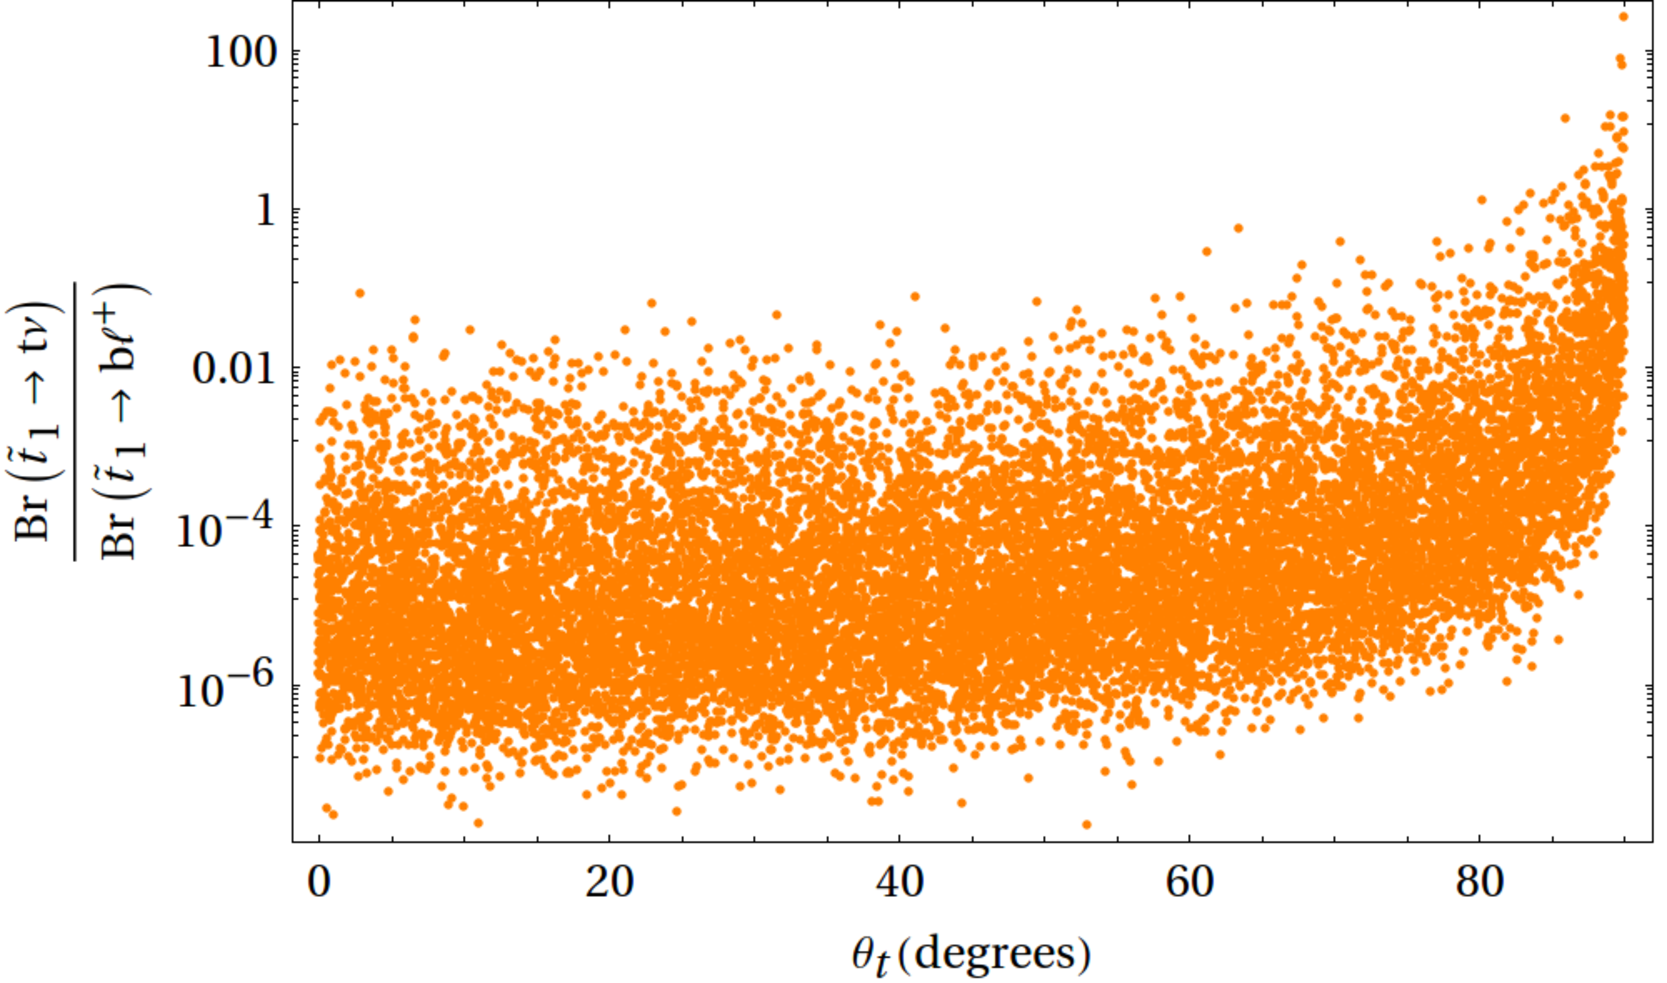
\includegraphics[width=0.70\textwidth]{figs/theory/StopBranchingRatiosVsMixingAngle.pdf}
      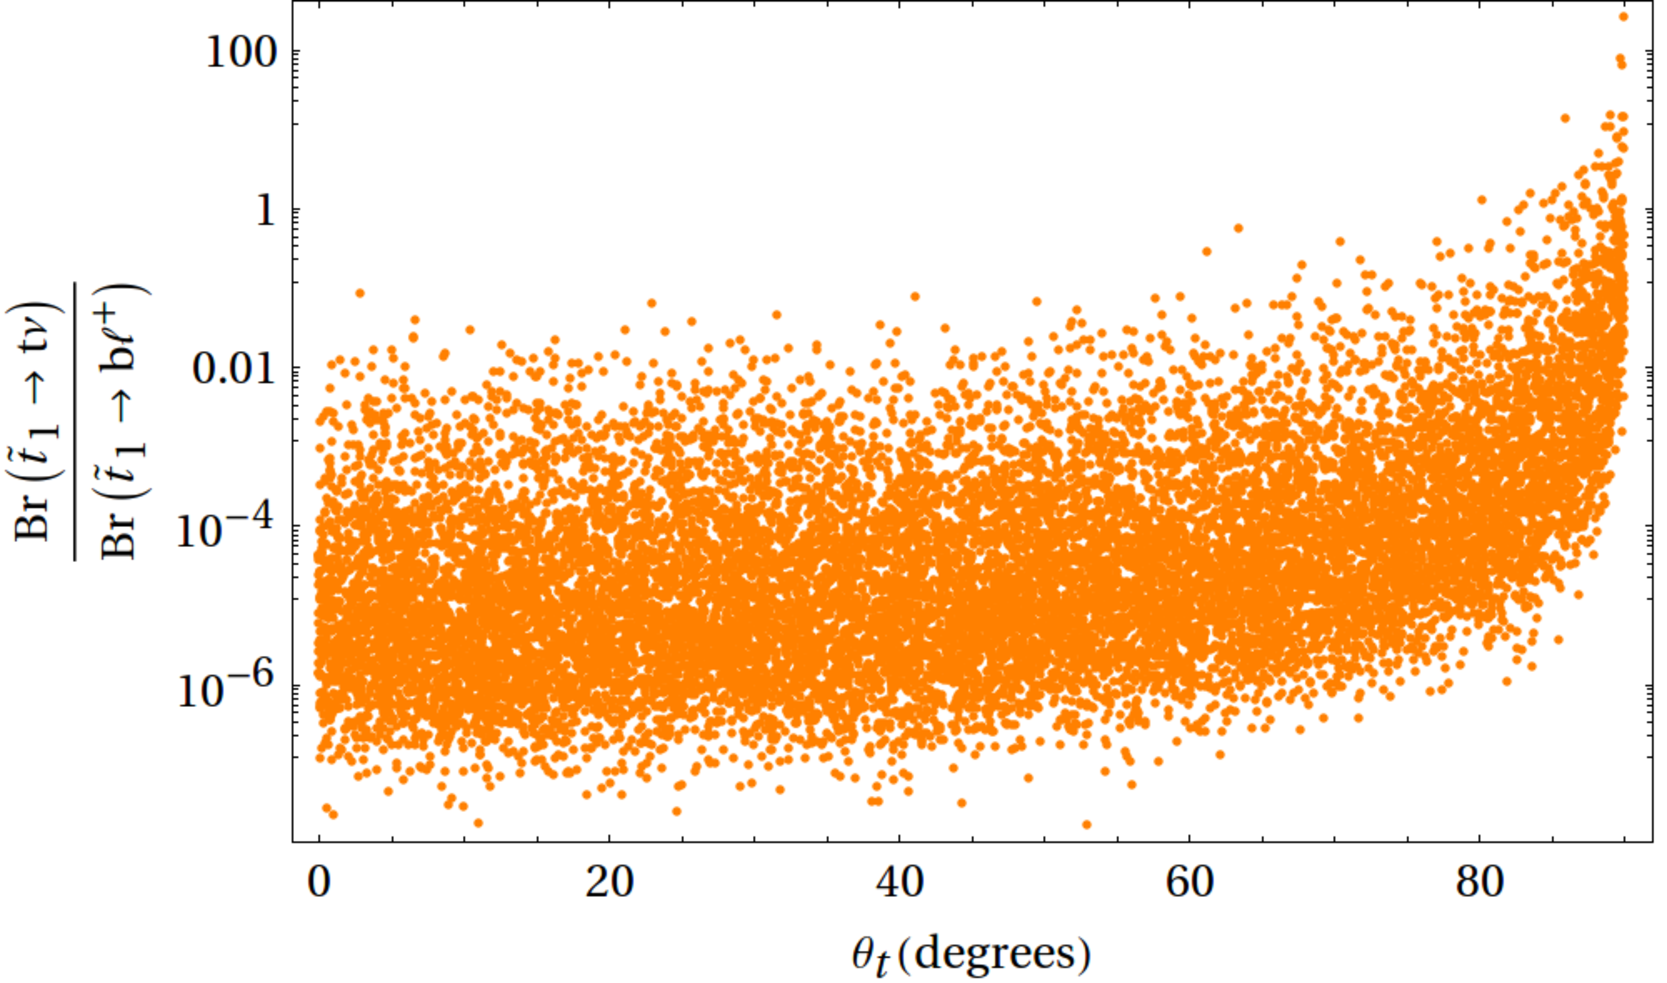
\includegraphics[width=\textwidth]{figs/theory/StopBranchingRatiosVsMixingAngle.pdf}
      \label{fig:stop_br_vs_mixing_angle}
    }
    \subbottom[Stop decay length]{
      % 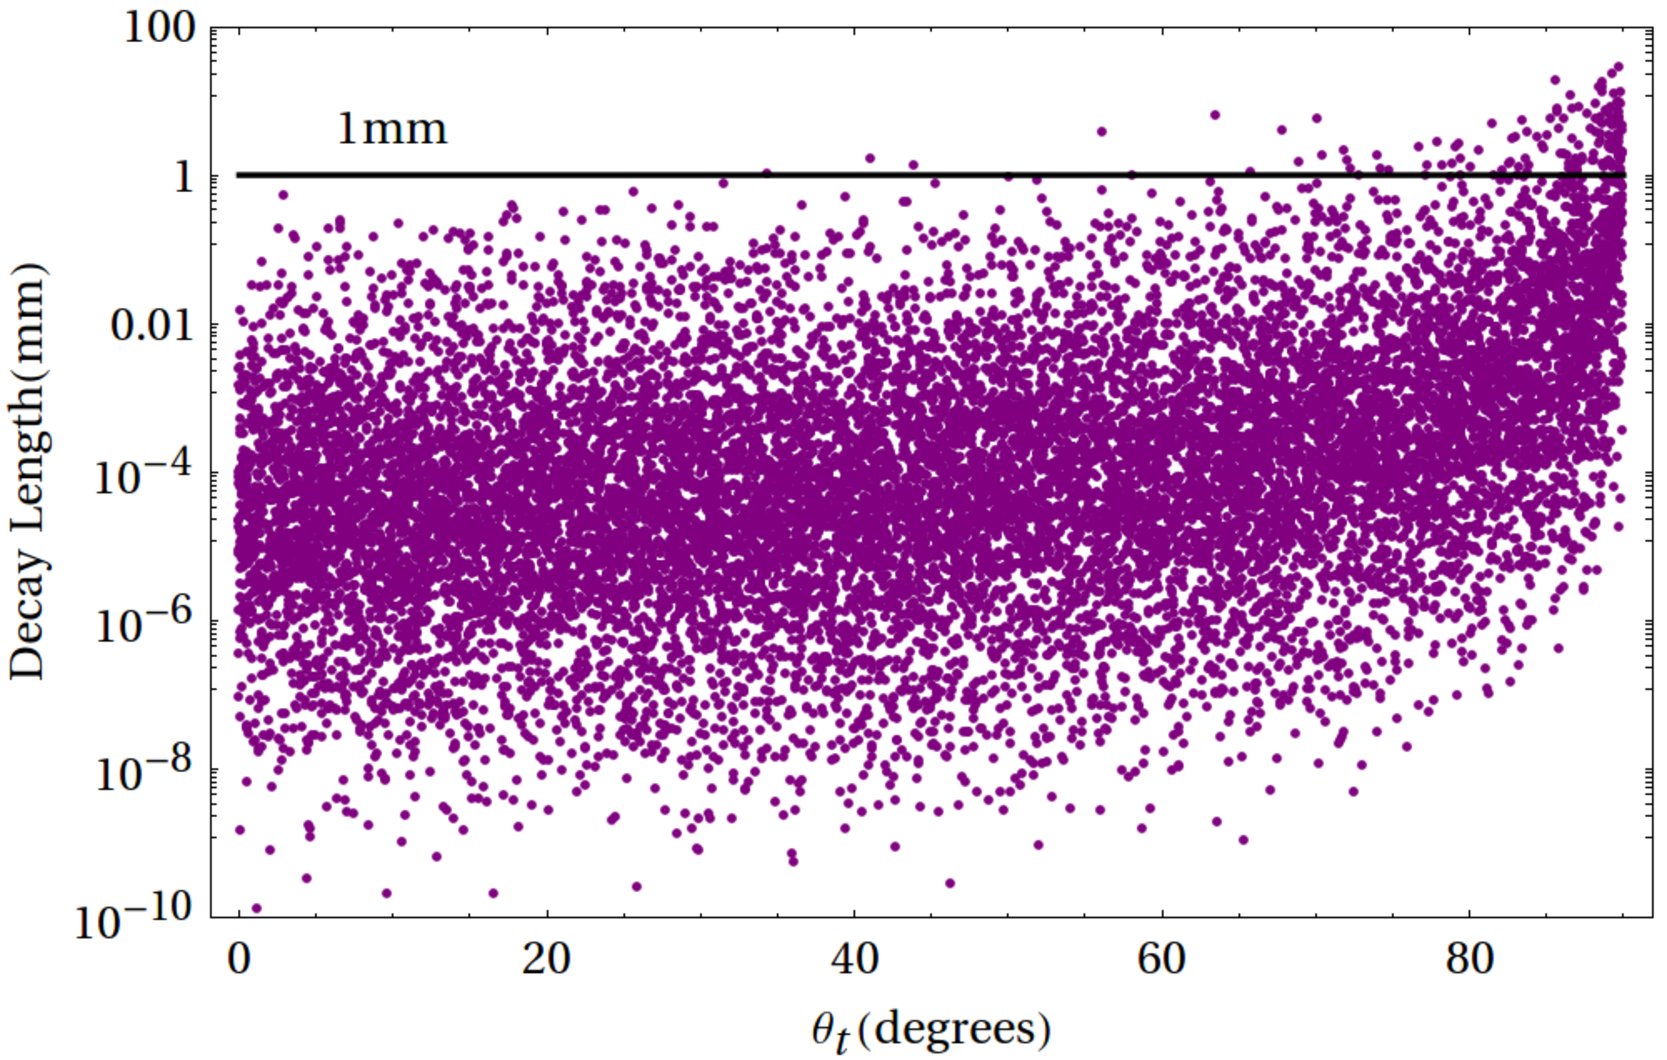
\includegraphics[width=0.70\textwidth]{figs/theory/DecayLength.pdf}
      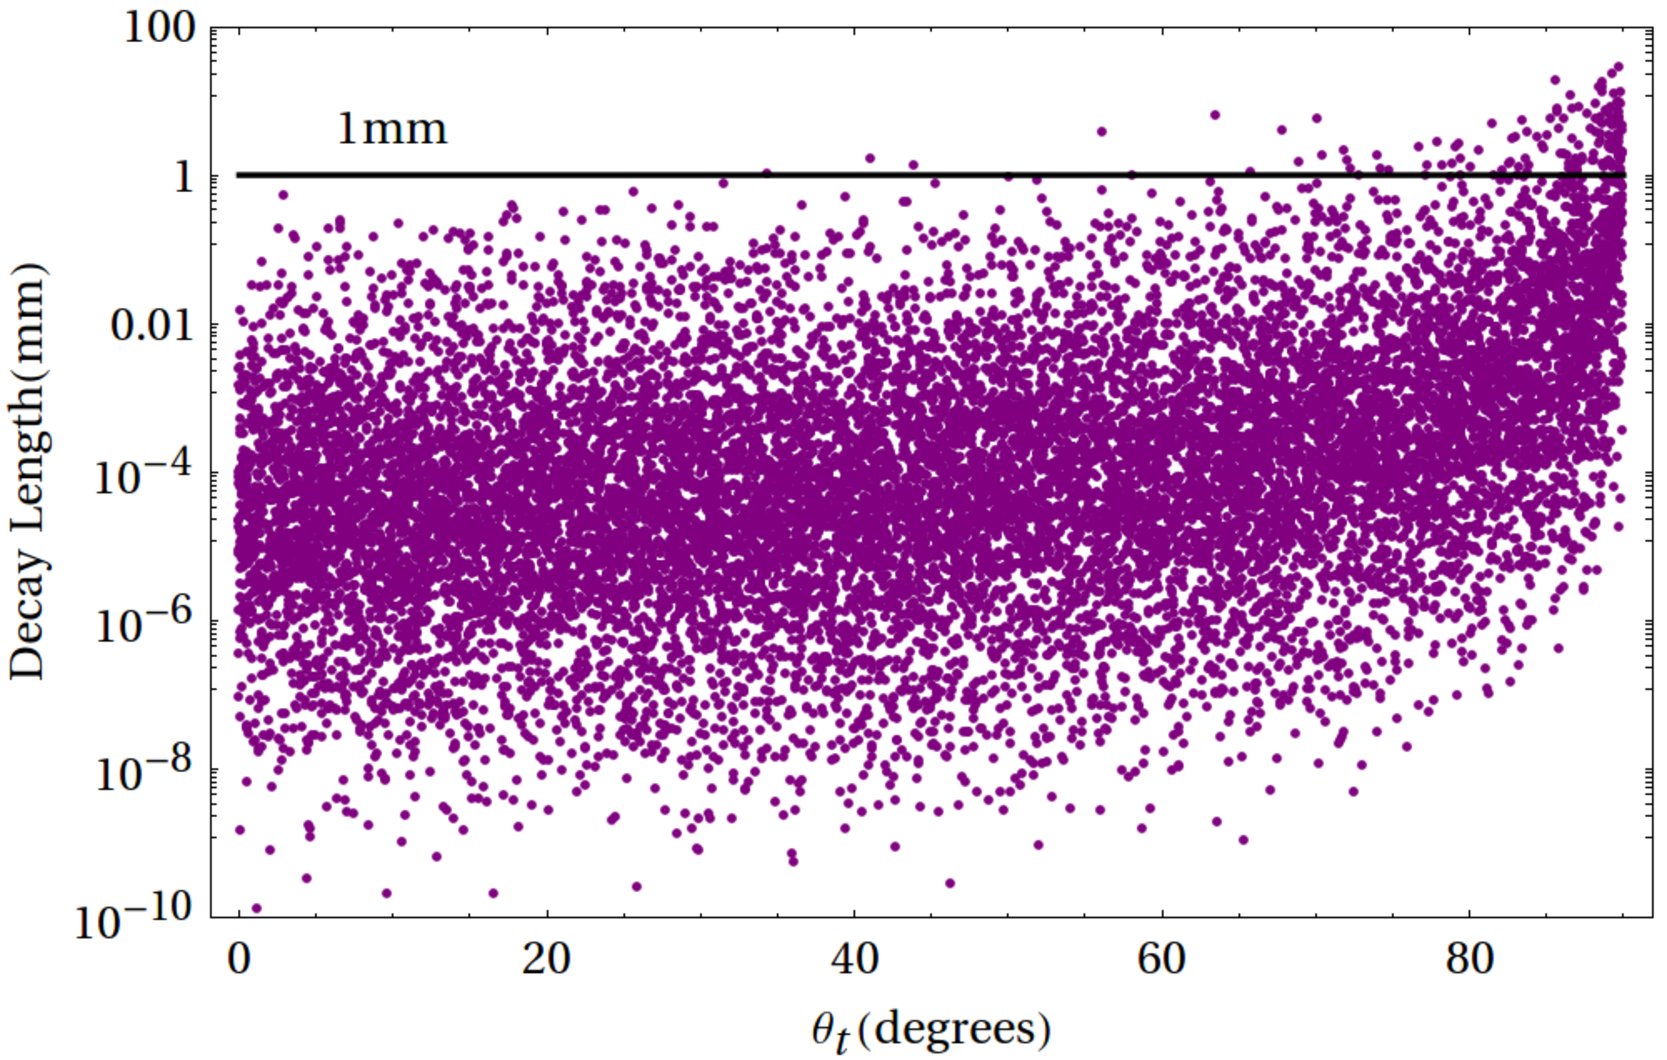
\includegraphics[width=\textwidth]{figs/theory/DecayLength.pdf}
      \label{fig:stop_decay_length_vs_mixing_angle}
    }
    \caption{These plots show the stop decay length and branching ratio versus
      the stop mixing angle, assuming the stop is the LSP.
      Each point in these plots represent a simulation with a particular
      choice of model parameters, which are varies within a range of natural
      values~\cite{Marshall:2014cwa}.
    }
    \label{fig:stop_vs_mixing_angle}
  }
\end{figure}

The analysis described in this thesis focuses on the $\stop \to b\ell$ decay
as it is preferred for most of parameter space.
Additionally, if the $\stop \to t\nu$ decay is significant, the decay of stop
pairs would lead to final states with $t\bar{t}$ associated with large missing
energy, which is the same final state as stop pair production with
$R$-Parity conserving decays, and the limits from traditional stop searches can
be reinterpreted for this model.

It is also reasonable to assume the stop decays in this model are prompt, and
decay with a negligible impact parameter, as shown in
Figure~\ref{fig:stop_decay_length_vs_mixing_angle}, where for most natural
models, the stop is expected to have a decay length of less than
$10^{-3}~\mathrm{mm}$;
in particular, this is true for models where the stop is not mostly
right-handed ($\theta_t \leq 80$)~\cite{Marshall:2014cwa,Marshall:2014kea}.
Therefore, long-lived particles are not considered in this analysis.

In this $B-L$ extension to the MSSM, stop pair production has the same
production cross section as in the traditional MSSM.
The expected production cross section are shown in Figure~\ref{fig:stop_xsec}.

\begin{figure}[ht]
  \centering{
    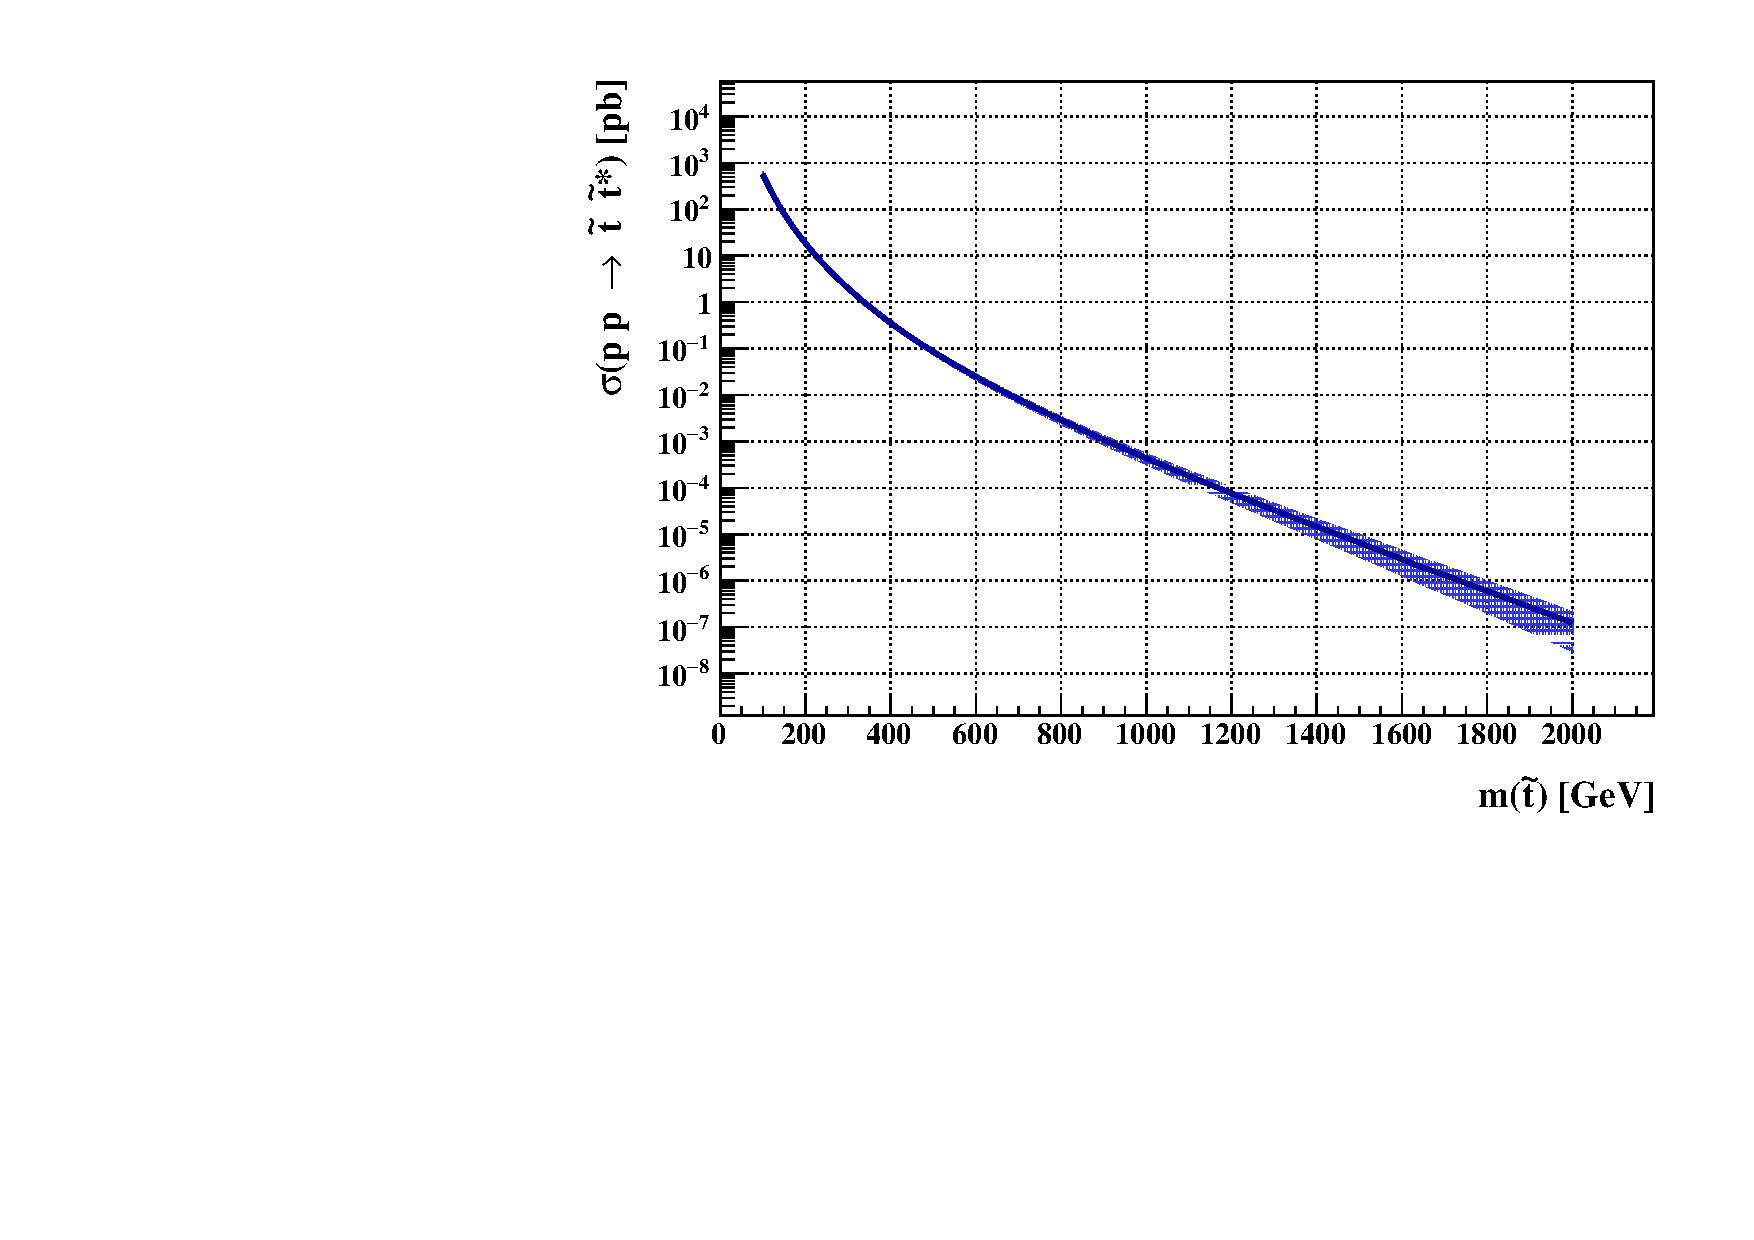
\includegraphics[width=\textwidth]{figs/theory/xsec.pdf}
  }
  \caption{Stop cross sections and their associated
    uncertainties~\cite{Beenakker:1997ut,Beenakker:2010nq,Beenakker:2011fu}.
  }
  \label{fig:stop_xsec}
\end{figure}

% %% -----------------------------------------------------------------------------
% \FloatBarrier
% \subsection{Expected kinematics}
% 
% {\color{red} TODO talk about expected event kinematics at truth level}
% 
% The expected event kinematics are studied using Monte Carlo (MC) simulation.
% Simulated stop pair production events are generated using \madgraph\ version
% 1.5.12~\cite{Alwall:2011uj} and \pythia\ version 6.427~\cite{Sjostrand:2006za},
% and the expected event kinematics are studied at the truth level, ignoring
% detector effects and potential inefficiencies.
% The simulated signal event generation procedure is described in more detail in
% Section~\ref{sec:mc_samples}.
% For illustration purposes, three choices of stop mass (100~\GeV, 500~\GeV,
% and 1000~\GeV), are compared in this section to give a picture of how the event
% kinematics are expected to evolve with increasing stop mass.
% 
% Figure~\ref{fig:truth_stop_pt} shows the expected 

%% -----------------------------------------------------------------------------
\FloatBarrier
\subsection{Previous results}

The results from existing leptoquark searches performed at ATLAS were
re-interpreted in the context of this $B-L$ SUSY model with a stop LSP, and the
limits obtained on the minimum allowable stop mass across the plane of
physical stop branching ratios are shown in
Figure~\ref{fig:pheno_limit}~\cite{Marshall:2014cwa,Marshall:2014kea}.
The leptoquark searches, used to obtain these mass limits, searched for
models where the decay products are in the same generation.
As a result, $b$-tagging is only required in events associated with a $\tau$
lepton, and events with a light lepton simply require a jet, regardless of the
flavor.
Additionally, previous leptoquark searches only consider decays to a single
lepton flavor, resulting in final states with either two leptons of the same
flavor and two jets, or a single charged lepton and at least one jet.
The previous analyses did not consider final states with two charged leptons
with different flavors ($e\mu$) and at least two 
jets~\cite{ATLAS:2013oea, ATLAS:2012aq, Aad:2011ch, CMS:2014qpa,
  Chatrchyan:2012sv, Chatrchyan:2012vza, Chatrchyan:2012st}.
A dedicated search requiring $b$-tagged jets associated with light leptons
(electrons and muons), and considering different flavored leptons in the final
state can provide additional sensitivity to this model, as well as other models
which result in final states with $b$-quarks and light leptons in the final
state.

\begin{figure}[p]
  \centering{
    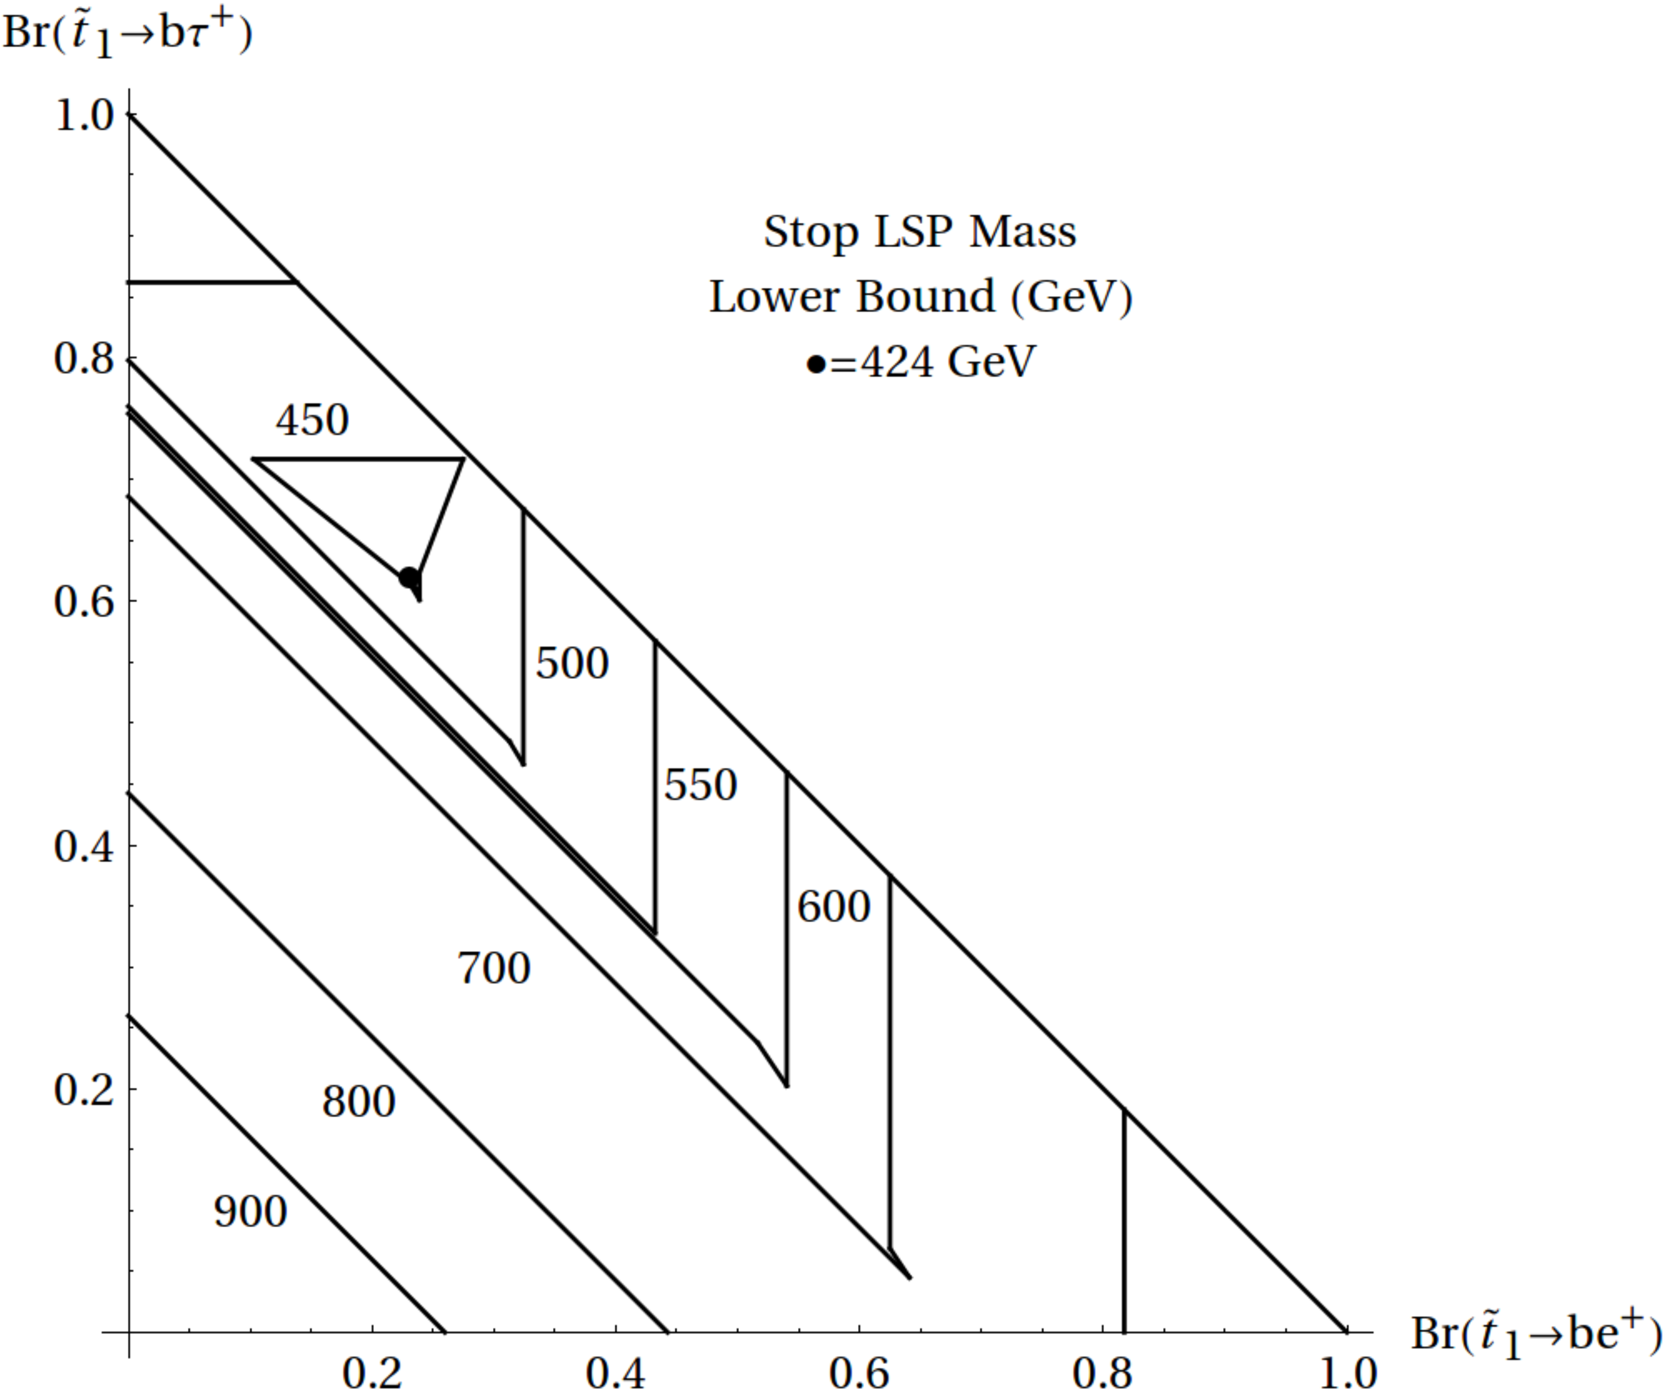
\includegraphics[width=\textwidth]
    {figs/theory/BoundContourPlotNoCombination.pdf}
    \caption{Limits on the stop mass obtained by reinterpreting leptoquark
      searches performed at ATLAS.
      The mass limits assume the stop is the LSP, and decays to a $b$-quark
      and a lepton~\cite{Marshall:2014cwa}.
    }
    \label{fig:pheno_limit}
  }
\end{figure}


%% \chapter[htoc-titlei][hhead-titlei]{htitlei}
%% -----------------------------------------------------------------------------
\chapter[The LHC and the ATLAS experiment][The LHC and ATLAS]
        {The LHC and the ATLAS experiment}

%% ------------------------------------------------------------------------------
\section{The LHC}

{\color{red}Standard boring stuff about the LHC accelerator complex, and there
  are four major experiments, blah blah blah. This shouldn't be too long}

%% ------------------------------------------------------------------------------
\section{The ATLAS experiment}

{\color{red} Brief intro to ATLAS before getting into the details}

%% - - - - - - - - - - - - - - - - - - - - - - - - - - - - - - - - - - - - - - -
\subsection{Inner detector} 

{\color{red} Introduce the ID and its purpose}

%% - - - - - - - - - - - - - - - - - - - - - - - - - - - - - - - - - - - - - - -
\subsubsection{Pixel detector} 

%% - - - - - - - - - - - - - - - - - - - - - - - - - - - - - - - - - - - - - - -
\subsubsection{Silicon semiconductor tracker} 

%% - - - - - - - - - - - - - - - - - - - - - - - - - - - - - - - - - - - - - - -
\subsubsection{Transition radiation tracker} 

{\color{red} Brief intro to TRT. Say more is coming later in
  Chapter~\ref{ch:trt}}

%% - - - - - - - - - - - - - - - - - - - - - - - - - - - - - - - - - - - - - - -
\subsection{Calorimetry} 

{\color{red} Introduce the calo systems and its purpose}

%% - - - - - - - - - - - - - - - - - - - - - - - - - - - - - - - - - - - - - - -
\subsubsection{Electromagnetic calorimeter} 

%% - - - - - - - - - - - - - - - - - - - - - - - - - - - - - - - - - - - - - - -
\subsubsection{Hadronic calorimeter} 

%% - - - - - - - - - - - - - - - - - - - - - - - - - - - - - - - - - - - - - - -
\subsection{Muon spectrometer} 

{\color{red} Introduce the MS and its purpose}

%% ------------------------------------------------------------------------------
\section{Triggering system}

{\color{red} Why/how we trigger. What sort of rates we get. What is the
rejection rate at each trigger level...}

%% ------------------------------------------------------------------------------
\section{Event reconstruction and object identification}

%% - - - - - - - - - - - - - - - - - - - - - - - - - - - - - - - - - - - - - - -
\subsection{Electrons} 

%% - - - - - - - - - - - - - - - - - - - - - - - - - - - - - - - - - - - - - - -
\subsection{Muons} 

%% - - - - - - - - - - - - - - - - - - - - - - - - - - - - - - - - - - - - - - -
\subsection{Jets} 

%% - - - - - - - - - - - - - - - - - - - - - - - - - - - - - - - - - - - - - - -
\subsection{Flavor tagging} 

%% - - - - - - - - - - - - - - - - - - - - - - - - - - - - - - - - - - - - - - -
\subsection{Missing energy} 

{\color{red} missing momentum?}

% %% \chapter[htoc-titlei][hhead-titlei]{htitlei}
%% -----------------------------------------------------------------------------
\chapter[The transition radiation tracker][The transition radiation tracker]
        {The transition radiation tracker}
\label{ch:trt}

{\color{red} Probably rename if I only talk about timing...}

%% -----------------------------------------------------------------------------
\section{TRT timing resolution}

{\color{red}Summarize my work on TRT timing resolution. I need to go back and
  review this! Talk about event time, etc.}


%% \chapter[htoc-titlei][hhead-titlei]{htitlei}
%% -----------------------------------------------------------------------------
\chapter[Monte Carlo simulation][Monte Carlo simulation]{Monte Carlo simulation}
\label{ch:mc}

Monte Carlo (MC) simulations are an important tool for particle physics
experiments.
MC techniques are used to simulate physics processes that occur during
particle collisions.
These simulated events also include the interactions of the decay products
in the detector, and can be used to tune the selection of an analysis,
estimate the expected event yields and kinematic shapes, and ultimately,
evaluate the expected sensitivity of a particular search.
MC simulation of background and signal processes are used on ATLAS.
This chapter introduces some of the basic concepts of event generation, but
focuses on the generation of the $B-L$ stop pairs from the model described in
Section~\ref{sec:theory_bl_extension}.

MC simulation of particle physics events can be broken into two major parts.
The first step is the event generation, described in
Section~\ref{sec:event_gen}.
In the event generation stage, the actual Physics processes that occur as a
result of the collision are simulated.
This includes the hard interaction as well as the resulting decay of any
unstable particles.
As in the real detector, once the proton collisions are simulated, the decay
products travel through the detector, and may leave a measurable signature
which can be measured.
This involved material interactions with the detector, and is discussed in
Section~\ref{sec:det_sim}.

%% -----------------------------------------------------------------------------
\FloatBarrier
\section{Event Generation}
\label{sec:event_gen}

Before discussing the details of event generation, it is useful to first
introduce the concept of an ``event.''
At the LHC, beams of protons are accelerated in opposite directions, and
allowed to cross at specific locations as described in Section~\ref{sec:lhc}.
At each of these crossings, protons from the two beams collide with one
another, resulting in a spray of particles in the detector.
Each of these crossings represents a single event.
Figure~\ref{fig:mc_event} shows a pictorial representation of a simulated
$t\bar{t}H$ event.

\begin{figure}[p]
  \centering
  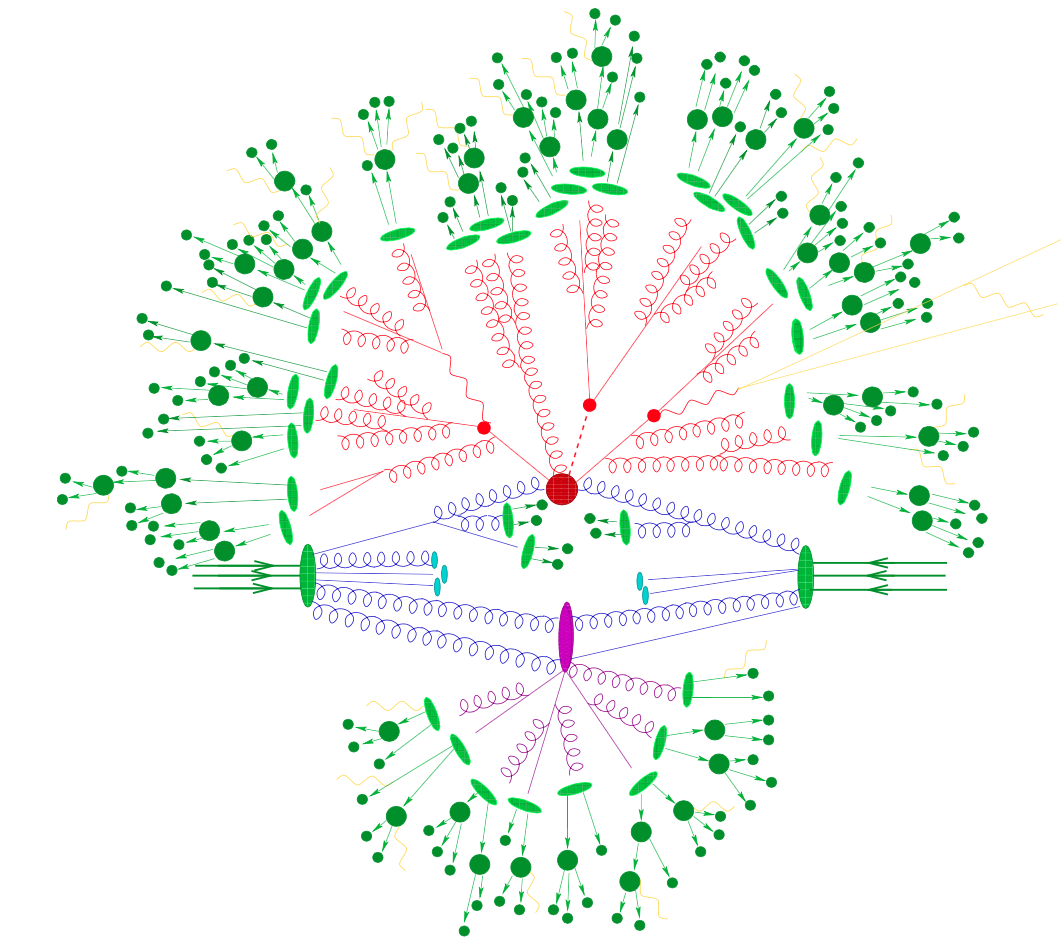
\includegraphics[width=\textwidth, clip=true, trim=0 0 0 0]
  {figs/mc_gen/full_mc_event.png}
  \caption[
    Pictorial representation of a $t\bar{t}H$ event as produced by an event
    generator~\cite{Gleisberg:2008ta}.
  ]{
    Pictorial representation of a $t\bar{t}H$ event as produced by an event
    generator.
    The hard interaction (big red blob) is followed by the decay of both top
    quarks and the Higgs boson (small red blobs).
    Additional hard QCD radiation is produced (red) and a secondary
    interaction takes place (purple blob) before the final-state partons
    hadronize (light green blobs) and hadrons decay (dark green blobs).
    Photon radiation occurs at any stage (yellow)~\cite{Gleisberg:2008ta}.
  }
  \label{fig:mc_event}
\end{figure}

Looking more closely at the interactions taking place, one notices that,
rather than the full protons interacting with each other, the interactions
take place between the constituent quarks and gluons within the two protons.
In some cases, there is a ``hard interaction,'' or an inelastic scattering
where additional particles are created.
This is mathematically represented by the ``matrix element'' calculation.
As the protons pass through each other, there are also soft interactions
between the constituent partons in a process called the ``underlying event.''
The underlying event produces charged particles and jets in the detector, in
addition to those coming from the hard interaction.

%% - - - - - - - - - - - - - - - - - - - - - - - - - - - - - - - - - - - - - - -
\FloatBarrier
\subsection{Underlying event}

%% - - - - - - - - - - - - - - - - - - - - - - - - - - - - - - - - - - - - - - -
\FloatBarrier
\subsection{Matrix element}

%% - - - - - - - - - - - - - - - - - - - - - - - - - - - - - - - - - - - - - - -
\FloatBarrier
\subsection{Parton shower}

%% - - - - - - - - - - - - - - - - - - - - - - - - - - - - - - - - - - - - - - -
\FloatBarrier
\subsection{Jet matching}
\label{sec:jet_matching}

{\color{red} Talk about matching. Probably use several figures to help explain
  this topic. Probably also talk about these DJR plots, and how we want them
  to look}

{\color{red} Add info about HFOR here}

%% -----------------------------------------------------------------------------
\FloatBarrier
\section{Detector simulation}
\label{sec:det_sim}

{\color{red} Probably something brief about how detector simulation is done, and
  the difference between full/fast sim}


%% \chapter[htoc-titlei][hhead-titlei]{htitlei}
%% -----------------------------------------------------------------------------
\chapter[B-L stop search][B-L stop search]{B-L stop search}
\label{ch:bl_stop}

In this chapter, a search is presented for the direct scalar top (stop) pair
production where the stops decay via an RPV coupling to a final state with two
leptons and two identified $b$-jets, show in Figure~\ref{fig:blstop_diagram}.
The motivation and phenomenology of this model is described further in
Section~\ref{sec:theory_bl_extension}.
20.3~\ifb of $\sqrt{s} = 8\TeV$ proton-proton collision data collected with the
ATLAS detector at the LHC is analyzed for this search.

This analysis required the generation of simulated signal Monte Carlo 
(Section~\ref{sec:signal_model_mc}) to develop the selection criteria, and
determine the expected sensitivity for the signatures of interest.
The object definitions, event cleaning, and trigger selections are described in
\cref{sec:object_selection,sec:event_cleaning,sec:trigger_selection}.
A "cuts-based" selection criteria is used to achieve a large separation between
signal-like processes and Standard Model (SM) background processes.
Two signal regions, expected to have a high signal-to-background ratio are
defined in Section~\ref{sec:signal_regions}, and used to assess the
compatibility of the data with the prediction from the target signal model,
compared with that of the SM prediction alone.
The background estimate is performed using MC simulation of SM processes, with
the normalizations taken from the observed yields in dedicated Control Regions,
defined in Section~\ref{sec:cr}, using a maximum likelihood fit, described in
Section~\ref{sec:bkg_fit}.
The extrapolation of the background estimate from the Control Regions to other
regions in kinematic space are validated in several Validation Regions.

The observed event yields in the Signal Regions are consistent with the SM
predictions, so limits are placed on the allowed stop masses and branching
ratios in Section~\ref{sec:results}.

% \begin{figure}[ht]
%   \centering
%   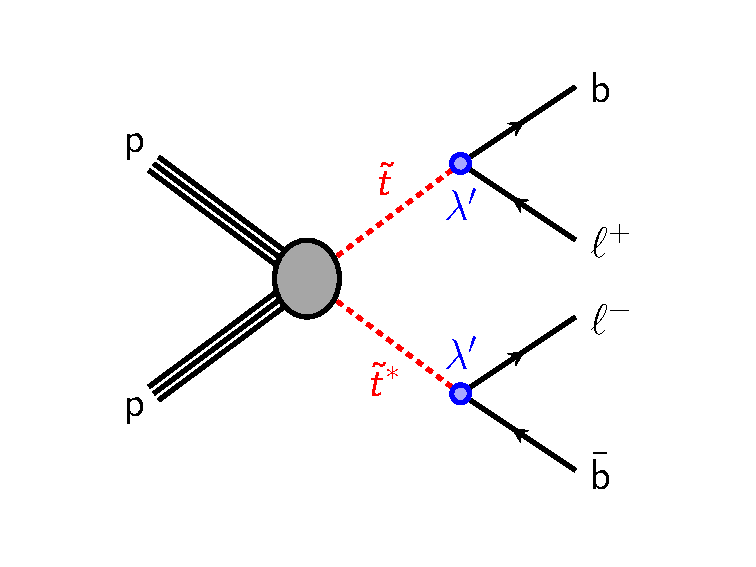
\includegraphics[width=0.60\textwidth]{figs/blstop/b_minus_l_stop_stop.pdf}
%   \caption{Simplified model of pair production of stop quarks, with decay to a
%     charged lepton and $b$-quark.
%   }
%   \label{fig:blstop_diagram}
% \end{figure}

%% -----------------------------------------------------------------------------
\FloatBarrier
\section{Signal model simulation}
\label{sec:signal_model_mc}

This search is optimized using Monte Carlo (MC) simulation of stop pair
production and decay.
Stop pair production is modeled using \madgraph\ version
1.5.12~\cite{Alwall:2011uj} to generate stop-anti-stop pairs using the
CTEQ 6L1 parton distribution functions (PDFs)~\cite{Nadolsky:2008zw},
and \pythia version 6.427~\cite{Sjostrand:2006za} to perform the
RPV stop decay as well as the parton shower calculation.
Stop pairs are generated for stop masses between 400~\GeV\ and 1100~\GeV\ in
steps of 100~\GeV.
Signal cross sections are calculated at next-to-leading order (NLO) in
$\alpha_s$, including the resummation of soft gluon emission at
next-to-leading-logarithm accuracy
(NLO+NLL)~\cite{Beenakker:1997ut,Beenakker:2010nq,Beenakker:2011fu}.
The nominal cross section and the uncertainty are taken from an envelope of
cross section predictions using different PDF sets and factorization and
renormalization scales, as described in Ref.~\cite{Kramer:2012bx}.
The simulated stop cross section ranges from $356 \pm 51$~fb for a stop mass
of 400~\GeV\ to $0.18 \pm 0.06$~fb for a stop mass of 1100~\GeV.
The cross sections and associated uncertainties for stop pair production are
summarized in Table~\ref{tab:stop_xsec}.

The simulated stop branching ratios in the MC simplified models is set to 
$Br(\tilde{t} \rightarrow be) = Br(\tilde{t} \rightarrow b\mu) = 0.5$.
The simulated events can be appropriately weighted to give any branching fraction
hypothesis.
Signal contributions from $\tilde{t} \rightarrow b\tau$ decays were shown not
to significantly contribute to the final state with two light leptons and two
$b$-jets.
This is due partially to the low branching ratio of leptonic tau decays (35\%
for each tau lepton), as well as the addition of a neutrino to the final state.
Because the decay $\tilde{t} \rightarrow b\tau$ does not significantly
contribute to the search sensitivity, is not included in the simulated
simplified model.

\begin{table}[ht]
  \caption{Stop cross sections and their associated
    uncertainties.~\cite{Beenakker:1997ut,Beenakker:2010nq,Beenakker:2011fu}.
  }
  \label{tab:stop_xsec}
  \centering{
    \begin{tabular}{cc}
      Stop Mass [\GeV] & Cross section [pb] \\
      \midrule
      400  & $0.36                \pm 0.05$               \\
      500  & $8.6  \times 10^{-2} \pm 1.3 \times 10^{-2}$ \\
      600  & $2.5  \times 10^{-2} \pm 4   \times 10^{-3}$ \\
      700  & $8.1  \times 10^{-3} \pm 1.5 \times 10^{-3}$ \\
      800  & $2.9  \times 10^{-3} \pm 6   \times 10^{-4}$ \\
      900  & $1.09 \times 10^{-3} \pm 2.6 \times 10^{-4}$ \\
      1000 & $4.4  \times 10^{-4} \pm 1.2 \times 10^{-4}$ \\
      1100 & $1.8  \times 10^{-4} \pm 6   \times 10^{-5}$ \\
      \bottomrule
    \end{tabular}
  }
\end{table}

%% -----------------------------------------------------------------------------
\FloatBarrier
\section{Object selection}
\label{sec:object_selection}

Events are required to have at least two light leptons (electrons or muons)
with opposite charge, and two $b$-tagged jets.
The object selection is performed in multiple steps. First, lepton and jet
objects are reconstructed using detector signatures as described in
Sections~\ref{sec:elctrons},~\ref{sec:muons},~and~\ref{sec:jets}.
Baseline requirements are applied to remove poorly reconstructed objects.
Also, all baseline objects are required to have $\ET(\pt) \geq 40 \GeV$ since the
stop signatures of interest tend to produce high momentum decay products.

%% - - - - - - - - - - - - - - - - - - - - - - - - - - - - - - - - - - - - - - -
%% baseline electrons
%% - - - - - - - - - - - - - - - - - - - - - - - - - - - - - - - - - - - - - - -
Baseline electrons must satisfy the \texttt{Medium++} identification
requirement and have $|\eta| \leq 2.47$.
A requirement of $\DZEROSIG \leq 3$ and $\ZZEROSINTHETA \leq 0.4$ mm
is placed on the impact parameter to reject electrons coming from secondary
vertices.
The baseline electron requirements are outlined in
Table~\ref{tab:baseline_el_def}.

\begin{table}[ht]
\caption{Baseline electron requirements.}
\label{tab:baseline_el_def}
\centering{
  \begin{tabular}{cc}
    \toprule
    Quality        & \texttt{Medium++} \\
    $p_T$          & $\geq 40 \GeV$    \\
    $|\eta|$       & $\leq 2.47$       \\
    \DZEROSIG      & $\leq 3$          \\
    \ZZEROSINTHETA & $\leq 0.4$ mm     \\
    \bottomrule
  \end{tabular}
}
\end{table}

%% - - - - - - - - - - - - - - - - - - - - - - - - - - - - - - - - - - - - - - -
%% baseline muons
%% - - - - - - - - - - - - - - - - - - - - - - - - - - - - - - - - - - - - - - -
Baseline muons are selected from the \texttt{STACO} muon collection, and
required to pass the \texttt{Loose} identification requirement. The baseline
muons must also have $|\eta| \leq 2.5$ 
Impact parameter requirements of $\DZEROSIG \leq 3$ and
$\ZZEROSINTHETA \leq 1$ mm are applied to reduce the contamination of muons
from secondary vertices and cosmic rays.
Additional requirements are applied on the number of hits in the ID to ensure
high quality tracks.
These  hit requirements include at least one hit on track in both the B layer
and the Pixel detector.
The ID track must also have at least 5 hits in the SCT, at most 2 missing 
hits-on-track (holes) in both the Pixel detector and the SCT. 
If the muon has $|\eta| \leq 1.9$, there must additionally be at least 6 TRT
hits, of which no more than 90\% are outliers.
Otherwise, no requirement is placed on the number of TRT hits.
The baseline muon requirements are outlined in Table~\ref{tab:baseline_mu_def}.

\begin{table}[ht]
  \caption{Baseline muon requirements.}
  \label{tab:baseline_mu_def}
  \centering{
    \begin{tabular}{cc}
      \toprule
      Quality              & \texttt{Loose} \\
      $p_T$                & $\geq 40 \GeV$ \\
      $|\eta|$             & $\leq 2.5$     \\
      Number B layer hits  & $\geq 1$       \\
      Number Pixel hits    & $\geq 1$       \\
      Number SCT hits      & $\geq 5$       \\
      Number Silicon holes & $\leq 2$       \\
      TRT hits             & See text       \\
      \DZEROSIG            & $\leq 3$       \\
      \ZZEROSINTHETA       & $\leq 1$ mm    \\
      \bottomrule
    \end{tabular}
  }
\end{table}

%% - - - - - - - - - - - - - - - - - - - - - - - - - - - - - - - - - - - - - - -
%% baseline jets
%% - - - - - - - - - - - - - - - - - - - - - - - - - - - - - - - - - - - - - - -
Baseline jets are selected from the AntiKt4LCTopo jet collection, and required
to have $|\eta| \leq 4.9$.
The baseline jet requirements are outlined in Table~\ref{tab:baseline_jet_def}.

\begin{table}[ht]
    \caption{Baseline jet requirements.}
    \label{tab:baseline_jet_def}
  \centering{
    \begin{tabular}{cc}
      \toprule
      $p_T$    & $\geq 40 \GeV$ \\
      $|\eta|$ & $\leq 4.9$     \\
      \bottomrule
    \end{tabular}
  }
\end{table}

%% - - - - - - - - - - - - - - - - - - - - - - - - - - - - - - - - - - - - - - -
%% overlap removal
%% - - - - - - - - - - - - - - - - - - - - - - - - - - - - - - - - - - - - - - -
After selecting baseline leptons and jets, overlap between baseline objects are
is removed to prevent a single detector signature from being included in
multiple particle collections. 

\begin{enumerate}
  \item $\Delta R(e,e) \le 0.05$: If two baseline electrons fall
    within a cone of $\Delta R(e,e) \le 0.05$, the electron with the
    lower \ET\ is removed from the event.
  \item $\Delta R(e,\mathrm{jet}) \le 0.20$: If a remaining electron and a jet
    are within a cone of $\Delta R(e,\mathrm{jet}) \le 0.20$, it is
    assumed that the electron is also reconstructed as a jet, and the
    jet is removed from the event.
  \item $\Delta R(\ell,\mathrm{jet}) \le 0.40$: If remaining lepton (electron
    or muon) and a remaining jet are within a cone of
    $\Delta R(\ell,\mathrm{jet}) \le 0.40$, the reconstructed lepton is assumed
    to be a constituent of the jet, and is removed from the event.
  \item $\Delta R(e,\mu) \le 0.01$: If a remaining electron and a remaining muon
    are within $\Delta R(e,\mu) \le 0.01$, both are removed from the event.
  \item $\Delta R(\mu,\mu) \le 0.05$: If two remaining muons are within
    $\Delta R(\mu,\mu) \le 0.05$, both are removed from the event.
\end{enumerate}

To reject leptons coming from low mass resonances, the invariant mass of any
remaining same-flavor lepton pairs with opposite charge is computed.
If the invariant mass of any of these pairs is less than 12~\GeV, both leptons
are removed from the event.

%% - - - - - - - - - - - - - - - - - - - - - - - - - - - - - - - - - - - - - - -
%% signal object definitions
%% - - - - - - - - - - - - - - - - - - - - - - - - - - - - - - - - - - - - - - -
Additional requirements are placed on the leptons and jets after overlap
removal to select the final ``signal'' objects.
The scalar sum of the momentum of all tracks with $\pt \geq 400 \GeV$
within a cone of $\Delta R \leq 0.30$ of a lepton ($\pt^\mathrm{cone30}$) is
used to determine if the lepton is isolated.
Both electrons and muons require
$\nicefrac{\pT^{\mathrm{cone30}}}{\min(p_T, 60 \GeV)} \leq 0.1$ in order
to be declared signal leptons.
Jets must pass a tighter cut of $|\eta| \leq 2.4$, and be tagged as a $b$-jet
according to the MV1 flavor tagging
algorithm~\cite{ATLAS-CONF-2014-004, ATLAS-CONF-2014-046}.
The operating point of $\mathrm{MV1} \geq 0.3511$ corresponds to an overall
80\% $b$-tagging efficiency, as measured in simulated \TTBAR\ events, to a
rejection factor of 25 for jets originating from light quarks or gluons, and to
a rejection factor of 3 for jets originating from charm quarks.

Events are required to have at least two signal leptons and two $b$-tagged jets.
If more are found, the event is kept, but only the two signal leptons and two
$b$-tagged jets with the highest \pt\ are selected.
Furthermore, the two highest \pt\ leptons are required to have opposite charge.

The identification efficiencies for the various objects used in this analysis
differ in the data and the MC simulation.
The efficiencies are determined in both data and MC simulation, and an
identification scale factor is applied to the MC simulation events to account
for the differences in identification efficiency.

The electron identification scale factors are provided by the Egamma combined
performance group, and depend on both the \et\ and \eta\ of the electrons within
a MC simulation event \cite{egamma2014}.
The scale factor is computed for each of the signal electrons in the event (at
most two), and the product of these scale factors is used as an event weight.
The muon identification scale factors follow the same procedure as the
electrons.
The muon scale factors, provided by the Muon combined performance group, depend
on both \pt\ and \eta, and are derived for each signal muon in the
event \cite{Aad:2014rra}.
The product of the muon identification scale factors is then taken as an
additional event weight.

A scale factor is applied to MC simulated events to match the probability of
tagging a $b$-jet correctly, and misidentifying jets originating from the
fragmentation of light-flavor quarks, gluons, and charm quarks. 
The scale factor depends on all the baseline jets in the event, and depends
on the \et, \eta, and truth flavor of each of the baseline jets in the
simulated event.
The scale factor for each individual jet is determined, and the overall
scale factor is given by
\begin{equation}
  \label{eqn:b_tag_sf}
  SF_{b\mathrm{-tagging}}^\mathrm{event} =
  \prod_{i \in \mathrm{tagged}}
  SF_i^\mathrm{eff}
  \times
  \prod_{j \in \mathrm{Not~tagged}}
  % SF_j^\mathrm{ineff},
  (1- SF_j^\mathrm{eff}),
\end{equation}
where $SF_i^\mathrm{eff}$ is the tagging efficiency scale factor of jet $i$, and
% $SF_j^\mathrm{ineff}$
$(1- SF_j^\mathrm{eff})$
is the rejection efficiency for jet $j$.
The two terms in equation~\ref{eqn:b_tag_sf}, are the products over the
$b$-tagged and non-$b$-tagged jets in the event respectively.
This $SF_{b\mathrm{-tagging}}^\mathrm{event}$ quantity is taken as an additional
event weight in MC simulated events.

%% - - - - - - - - - - - - - - - - - - - - - - - - - - - - - - - - - - - - - - -
%% pairing
%% - - - - - - - - - - - - - - - - - - - - - - - - - - - - - - - - - - - - - - -
To construct the mass of each of the $b\ell$ pairs, the leptons and $b$-tagged
jets must be paired.
It is possible to exploit the fact that in the target signal model, each
$b\ell$ pair comes from a resonant decay of a stop particle, and should
reconstruct the same invariant mass.
Therefore, the pairing which minimizes the difference in mass between the two
$b\ell$ pairs is selected as follows.

The two signal leptons and two $b$-jets are labeled $\ell_0$, $\ell_1$, $b_0$,
and $b_1$.

% Define some colors for this section to make changing colors easier
\colorlet{pairing_l_0}{green!50!white}
\colorlet{pairing_l_1}{green!20!white}
\colorlet{pairing_b_0}{red!50!white}
\colorlet{pairing_b_1}{red!20!white}
%
\begin{center}
  \begin{tikzpicture}
    \node[rectangle, rounded corners=1ex, fill=pairing_b_0, text=black]
      (b0) at (-3,0) {$b_0$};
    \node[rectangle, rounded corners=1ex, fill=pairing_b_1, text=black]
      (b1) at (-1,0) {$b_1$};
    \node[rectangle, rounded corners=1ex, fill=pairing_l_0, text=black]
      (l0) at (+1,0) {$\ell_0$};
    \node[rectangle, rounded corners=1ex, fill=pairing_l_1, text=black]
      (l1) at (+3,0) {$\ell_1$};
  \end{tikzpicture}
\end{center}
%
There are two possible choices of pairings for these four objects.
%
\begin{center}
  \begin{tikzpicture}
    \node[rectangle, text=black] (sel1) at (-5.0,+0.5) {Selection 1:};
    \node[rectangle, text=black] (sel2) at (-5.0,-0.5) {Selection 2:};

    \node[rectangle, rounded corners=1ex, fill=pairing_b_0, text=black]
      (b1) at (-3.25,+0.5) {$b_0$};
    \node[rectangle, rounded corners=1ex, fill=pairing_l_0, text=black]
      (l0) at (-2.50,+0.5) {$\ell_0$};
    \node[rectangle, rounded corners=1ex, fill=pairing_b_1, text=black]
      (b1) at (+1.25,+0.5) {$b_1$};
    \node[rectangle, rounded corners=1ex, fill=pairing_l_1, text=black]
      (l1) at (+2.00,+0.5) {$\ell_1$};
    \node[rectangle, text=black]
      (m00) at (-1.0,+0.5)
      {$\Rightarrow m_{b_0\ell_0} = m_{b\ell}^\mathrm{a}$};
    \node[rectangle, text=black]
      (m11) at (+3.5,+0.5)
      {$\Rightarrow m_{b_1\ell_1} = m_{b\ell}^\mathrm{b}$};

    \node[rectangle, rounded corners=1ex, fill=pairing_b_0, text=black]
      (b0) at (-3.25,-0.5) {$b_0$};
    \node[rectangle, rounded corners=1ex, fill=pairing_l_1, text=black]
      (l1) at (-2.50,-0.5) {$\ell_1$};
    \node[rectangle, rounded corners=1ex, fill=pairing_b_1, text=black]
      (b1) at (+1.25,-0.5) {$b_1$};
    \node[rectangle, rounded corners=1ex, fill=pairing_l_0, text=black]
      (l0) at (+2.00,-0.5) {$\ell_0$};
    \node[rectangle, text=black]
      (m01) at (-1.0,-0.5)
      {$\Rightarrow m_{b_0\ell_1} = m_{b\ell}^\mathrm{a} $};
    \node[rectangle, text=black]
      (m10) at (+3.5,-0.5)
      {$\Rightarrow m_{b_1\ell_0} = m_{b\ell}^\mathrm{b} $};
  \end{tikzpicture}
\end{center}

The masses of all pairings are calculated, and the pairing which gives the 
smallest difference in the mass $|\MBL^\mathrm{a} - \MBL^\mathrm{b}|$
is chosen.
The pairs are then ordered, and relabeled such that the higher mass pair has a
mass of $\MBL^{0}$, and the lower mass pair has a mass of $\MBL^{1}$.
This ensures $\MBL^{0} \geq \MBL^{1}$ by definition.

This heuristic correctly identifies at least one correct pairing of $b$-tagged
jets and leptons in roughly 65-90\% of events in the simulated signal samples
depending on the mass of the simulated stop. The efficiency, shown in
Figure~\ref{fig:pairing_eff}, improves once a cut is applied on the mass
asymmetry of the two $b\ell$ pairs as described in Section
\ref{sec:signal_regions}.

\begin{figure}[ht]
  \centering
  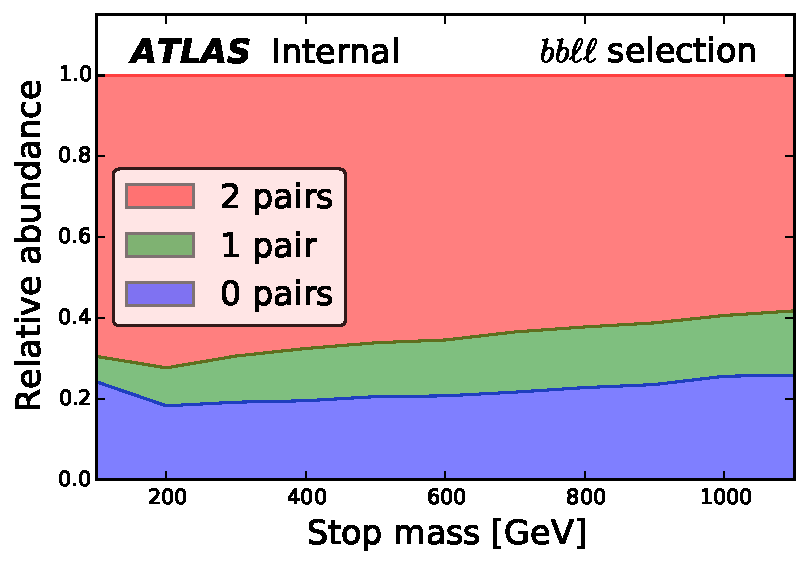
\includegraphics[width=0.60\textwidth]
    {figs/blstop/PairingEfficiencies/pairing_abundance__inclusive.pdf}
    % {figs/blstop/PairingEfficiencies/pairing_eff__inclusive.pdf}
  \caption{The relative abundance of each category of correctly pairing
    $b$-tagged jets and leptons using the pairing heuristic described in
    Section~\ref{sec:object_selection} for the different stop masses which are
    considered.
    The regions show the relative abundance of events where two, one, and zero
    pairs are grouped correctly.
    The scenario where one pair is identified correctly corresponds to events
    where one pair is grouped correctly, but at least of of the $b$-tagged jets
    or one of the leptons is not matched to a stop parent.
  }
  % \caption{The efficiency of correctly pairing $b$-tagged jets and leptons
  %   using the pairing heuristic described in Section~\ref{sec:object_selection}
  %   for the different stop masses which are considered.
  %   The different lines show the fraction of events where zero, one, or two
  %   pairs are grouped correctly.
  %   The scenario where one pair is identified correctly corresponds to events
  %   where one pair is grouped correctly, but at least of of the $b$-tagged jets
  %   or one of the leptons is not matched to a stop parent.
  % }
  \label{fig:pairing_eff}
\end{figure}

%% -----------------------------------------------------------------------------
\FloatBarrier
\section{Event cleaning}
\label{sec:event_cleaning}

All sub-systems of the ATLAS detector are required to be operating acceptably
during data-taking. 
This data quality requirement is implemented using a good runs list (GRL)
provided by the Data Preparation group.\footnote{The GRL version
\texttt{data12\_8TeV.periodAllYear\_DetStatus-v61-pro14-02\_DQDefects-00-01-00\_PHYS\_StandardGRL\_All\_Good}
is used.}
By applying the GRL requirement, the total integrated luminosity is reduced
from 21.4~\ifb\ to 20.3~\ifb.
The uncertainty on the luminosity is $\pm 2.8$\%.
It is derived following the same methodology as that detailed
in Ref.~\cite{Lumi}.
The GRL requirement is applied to data events only; the MC simulation samples
are scaled to match the target luminosity.

% Several other detector errors can lead to an event being rejected.
In the event of a certain detector busy condition, the TTC may be restarted in
order to recover the detector without a full run-restart. In the lumi-block
after a TTC restart, it is possible for stored events to be incomplete.
For this reason, events stored immediately after a TTC restart are rejected.
Furthermore, events are rejected if either the LAr or tile calorimeter is
flagged as having an error.
During periods G-J several events are corrupt in a single channel of the tile
calorimeter, but not flagged as having a tile calorimeter error.
These events are also rejected using the \texttt{TileTripTool}.
During period B a hot spot developed in the tile calorimeter.
As this can negatively impact the jet calibration and the \met calculations,
events with a jet pointing toward this hot spot in the tile calorimeter are
rejected.

Jet cleaning is performed to flag jets which are formed from various sources
such as hardware problems, LHC beam conditions, or cosmic ray showers rather
than real energy deposits in the calorimeter.
If any of these bad jets remain after the overlap removal procedure, the event
is rejected.
Additionally, during periods E-H, a region of the LAr
calorimeter ($-0.1\le\eta\le1.5$ and $-0.9\le\phi\le-0.5$) malfunctioned
resulting in a hole in the sub-detector.
This resulted in energy not being collected from electrons and jets close to
this hole, and indirectly changing the \met\ measurement.
A correction is applied to jets to account for the energy loss in the hole,
however, if the correction is too large (greater than 0.05) and the \met\ is
close to the jet ($\Delta\phi(\met, \text{jet}) \le 0.3$), it is assumed the
\met\ is mismeasured, and the event is rejected.

In addition to the impact parameter requirement on muons discussed in
Section~\ref{sec:object_selection}, an additional requirement of
$|d_0| \leq 0.2$~mm is applied to muons passing the overlap removal to reject
muons from cosmic rays. Any event failing this selection requirement is
rejected.
In order to ensure muons are well measured, any event containing a muon after
overlap removal with $\sigma_{q/p}/|q/p| > 0.2$ is rejected.
These poorly measured muons can arise from the MS and ID reconstructing
different momenta for the same muon.

Each event is also required to have at least one primary vertex with at least
5 associated tracks.

An additional requirement is applied to MC simulation events to avoid double
counting backgrounds with heavy flavor quarks in the final state, the heavy
flavor overlap removal procedure, described in Section~\ref{sec:jet_matching},
is applied.
{\color{red} This reference might belong to the MC section rather than jet
matching. TODO see what this ends up being.}

Events in data are taken from both the \texttt{egamma} and \texttt{muons} data
streams.
It is possible for the same event to exist in both streams, leading to the
possibility of double counting events.
To prevent this double counting of data events, the data stream is chosen based
on the flavor of the leading signal lepton in the event.
If the highest \pt\ event is an electron, the event is required to be found in
the \texttt{egamma} data stream.
Similarly, if the highest \pt\ lepton is a muon, the event is required to be
found in the \texttt{muons} data stream.
Events found in the wrong stream, are rejected.

%% -----------------------------------------------------------------------------
\FloatBarrier
\section{Trigger selection}
\label{sec:trigger_selection}

A combination of four single-lepton triggers are used to select events.
The specific triggers used depend on the flavor channel of the event.
Di-electron(muon) events are required to pass at least one of the two single
electron (muon) triggers, while electron-muon events may pass any one of the
four triggers.
The specific triggers used for each flavor channel are outlined in
Table~\ref{tab:triggers}, and the trigger requirements are described in
Table~\ref{tab:trigger_defs}.

\begin{table}[ht]
  % \caption{Trigger selection for each final state. If the event passes any of
  %   the triggers for the given final state, the event is accepted.
  % }
  \caption[Trigger selection for each final state.]{Trigger selection for each final state. If the event passes any of
    the triggers for the given final state, the event is accepted.
  }
  \label{tab:triggers}
  \centering{
    \begin{tabular}{cc}
      \toprule
      Final state & Trigger \\
      \midrule
      \multirow{2}{*}{$ee$bb}     &  \texttt{EF\_e24vhi\_medium1} \\
                                  &  \texttt{EF\_e60\_medium1}    \\
      \midrule
      $\mu\mu$bb                  &  \texttt{EF\_mu24i\_tight}    \\
      $\mu\mu$bb                  &  \texttt{EF\_mu36\_tight}     \\
      \midrule
      \multirow{3}{*}{$e\mu$bb}   &  \texttt{EF\_e24vhi\_medium1} \\
                                  &  \texttt{EF\_e60\_medium1}    \\
                                  &  \texttt{EF\_mu24i\_tight}    \\
                                  &  \texttt{EF\_mu36\_tight}     \\
      \bottomrule
    \end{tabular}
  }
\end{table}

\begin{table}[ht]
    \caption{Requirements for the triggers used in this analysis.  }
    \label{tab:trigger_defs}
  \centering{
    \begin{tabular}{c|cc}
      \toprule
      Trigger & \pt\ threshold & Other requirements \\
      \midrule
      \multirow{2}{*}{\texttt{EF\_e24vhi\_medium1}}
      & \multirow{2}{*}{$\pt^{e} \geq 24 \GeV$}
      & hadronic core isolation $\leq 1 \GeV$ \\
      & & $\nicefrac{\pt^\mathrm{cone20}}{\pt} < 0.1$ \\
      \texttt{EF\_e60\_medium1} & $\pt^{e} \geq 60 \GeV$ & -- \\
      \texttt{EF\_mu24i\_tight}
      & $\pt^{e} \geq 24 \GeV$
      & $\nicefrac{\pt^\mathrm{cone20}}{\pt} < 0.12$ \\
      \texttt{EF\_mu36\_tight}  & $\pt^{e} \geq 36 \GeV$ & -- \\
      \bottomrule
    \end{tabular}
  }
\end{table}

At least one of the reconstructed leptons is required to be within 
$\Delta R \leq 0.15$ of the detector signature found by the trigger.
The expected trigger efficiencies for simulated stop events are shown
for each trigger individually in Figure~\ref{fig:single_trigger_efficiency}.
The two muon triggers have roughly the same trigger efficiency, of about 93\% 
for $\mu\mu$ events and 75\% for $e\mu$ events, for all stop masses.
The two electron triggers, however, have dramatically different shapes, with
the \texttt{EF\_e24vhi\_medium1} trigger being highly efficient for $ee$ and
$e\mu$ events low mass from low mass stop, which decrease for higher
stop masses. 
The \texttt{EF\_e60\_medium1} trigger is not efficient for lower stop
masses, but quickly reaches approximately efficiencies above 95\% efficiency for
$ee$ and $e\mu$ events.

The dependence on the stop mass is a result of the \ET\ dependence of the
electron triggers.
The decay products of lighter stops tend to have lower momentum.
As a result, the electrons from the very light stops ($\leq 300~\GeV$) do not 
are more likely have \ET\ less than the threshold for the
\texttt{EF\_e60\_medium1} trigger.
Similarly, high-\HT\ electrons will deposit more energy into the calorimeter,
and some of this energy will reach the hadronic calorimeter.
As the electron \HT\ increases, the probability that the energy deposition into
the hadronic calorimeter is enough to fail hadronic core isolation requirement
of the \texttt{EF\_e24vhi\_medium1} trigger increases.
The \ET\ dependence of the two electron triggers, shown in
Figure~\ref{fig:electron_trigger_pt_dependence}, is consistent with the expected
dependence.

\begin{figure}[ht]
  \centering
  \subbottom[\texttt{EF\_e24vhi\_medium1}]{
    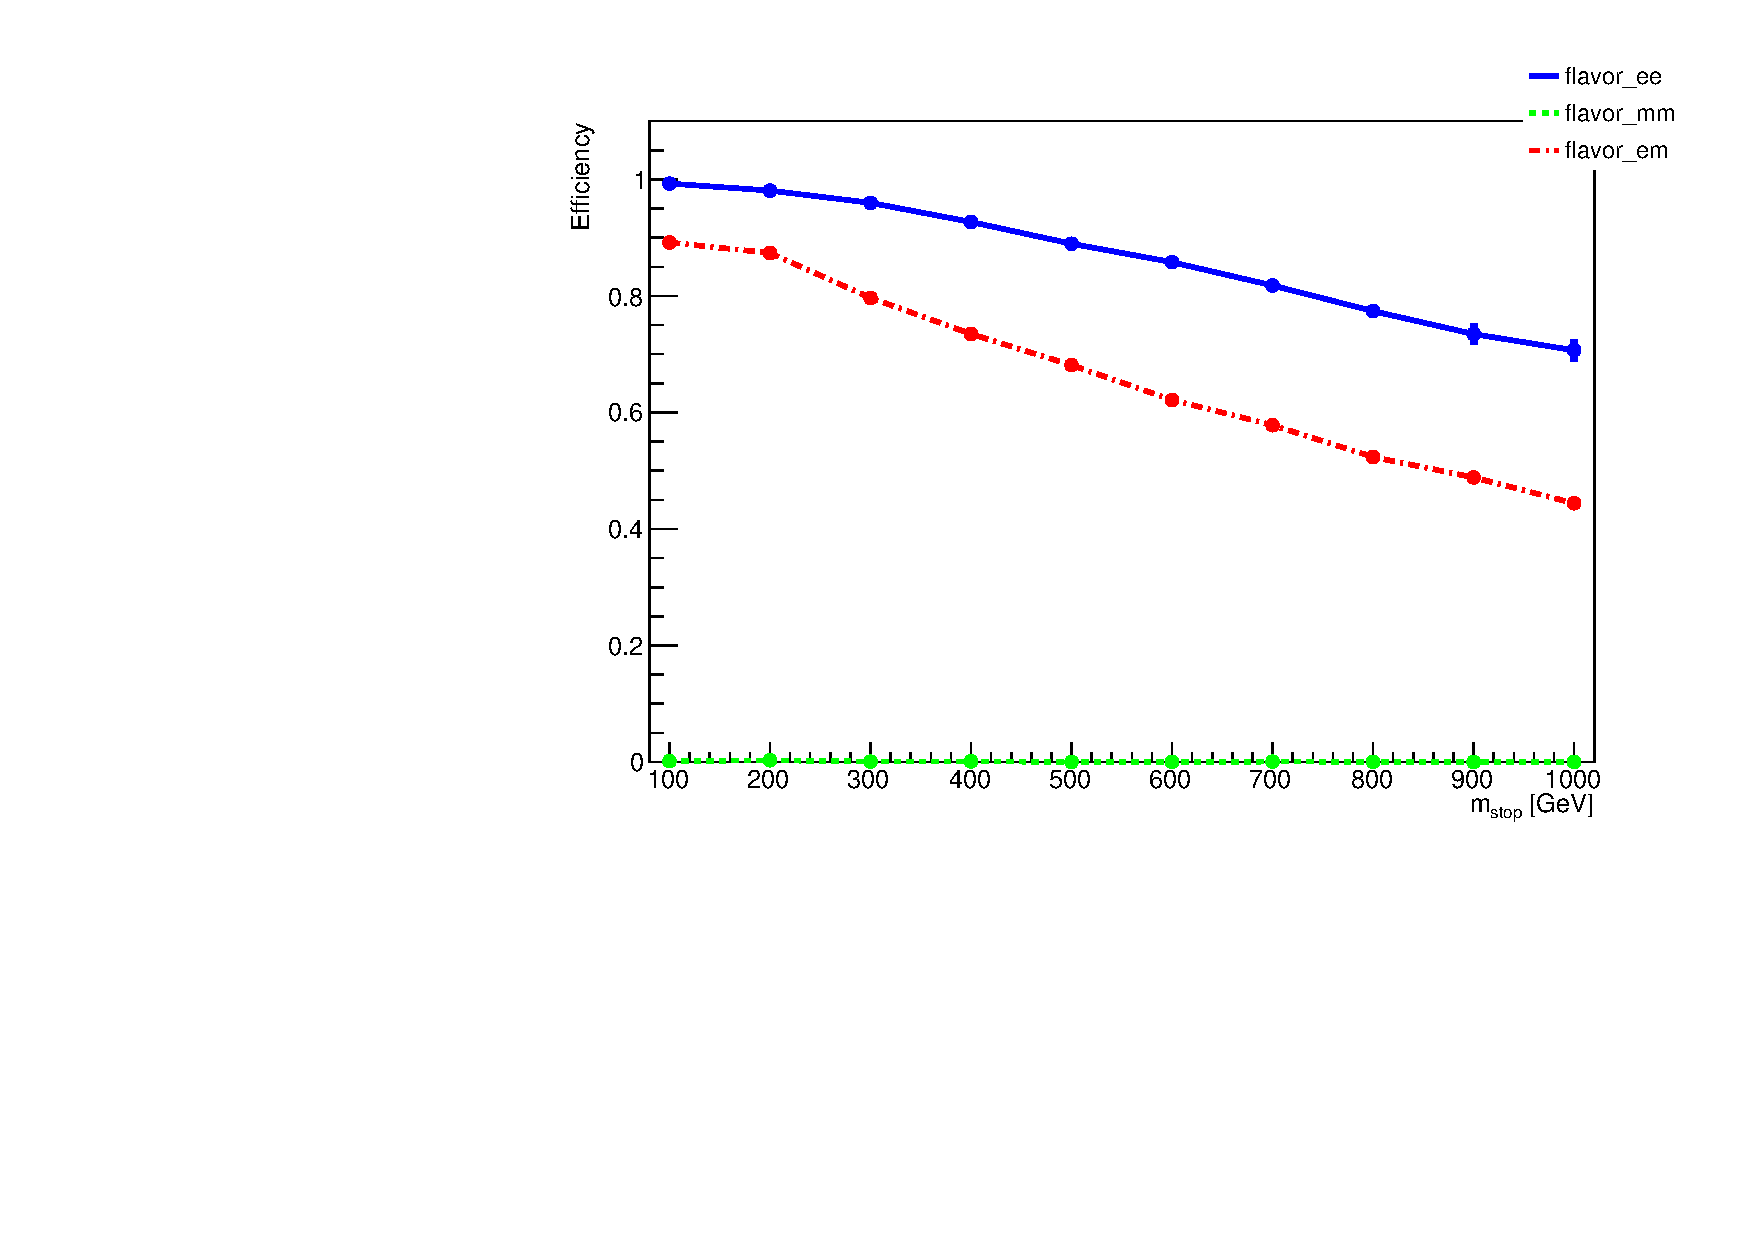
\includegraphics[width=0.48\textwidth]
      {figs/trigger/EF_e24vhi_medium1.pdf}
  }
  \subbottom[\texttt{EF\_e60\_medium1}]{
    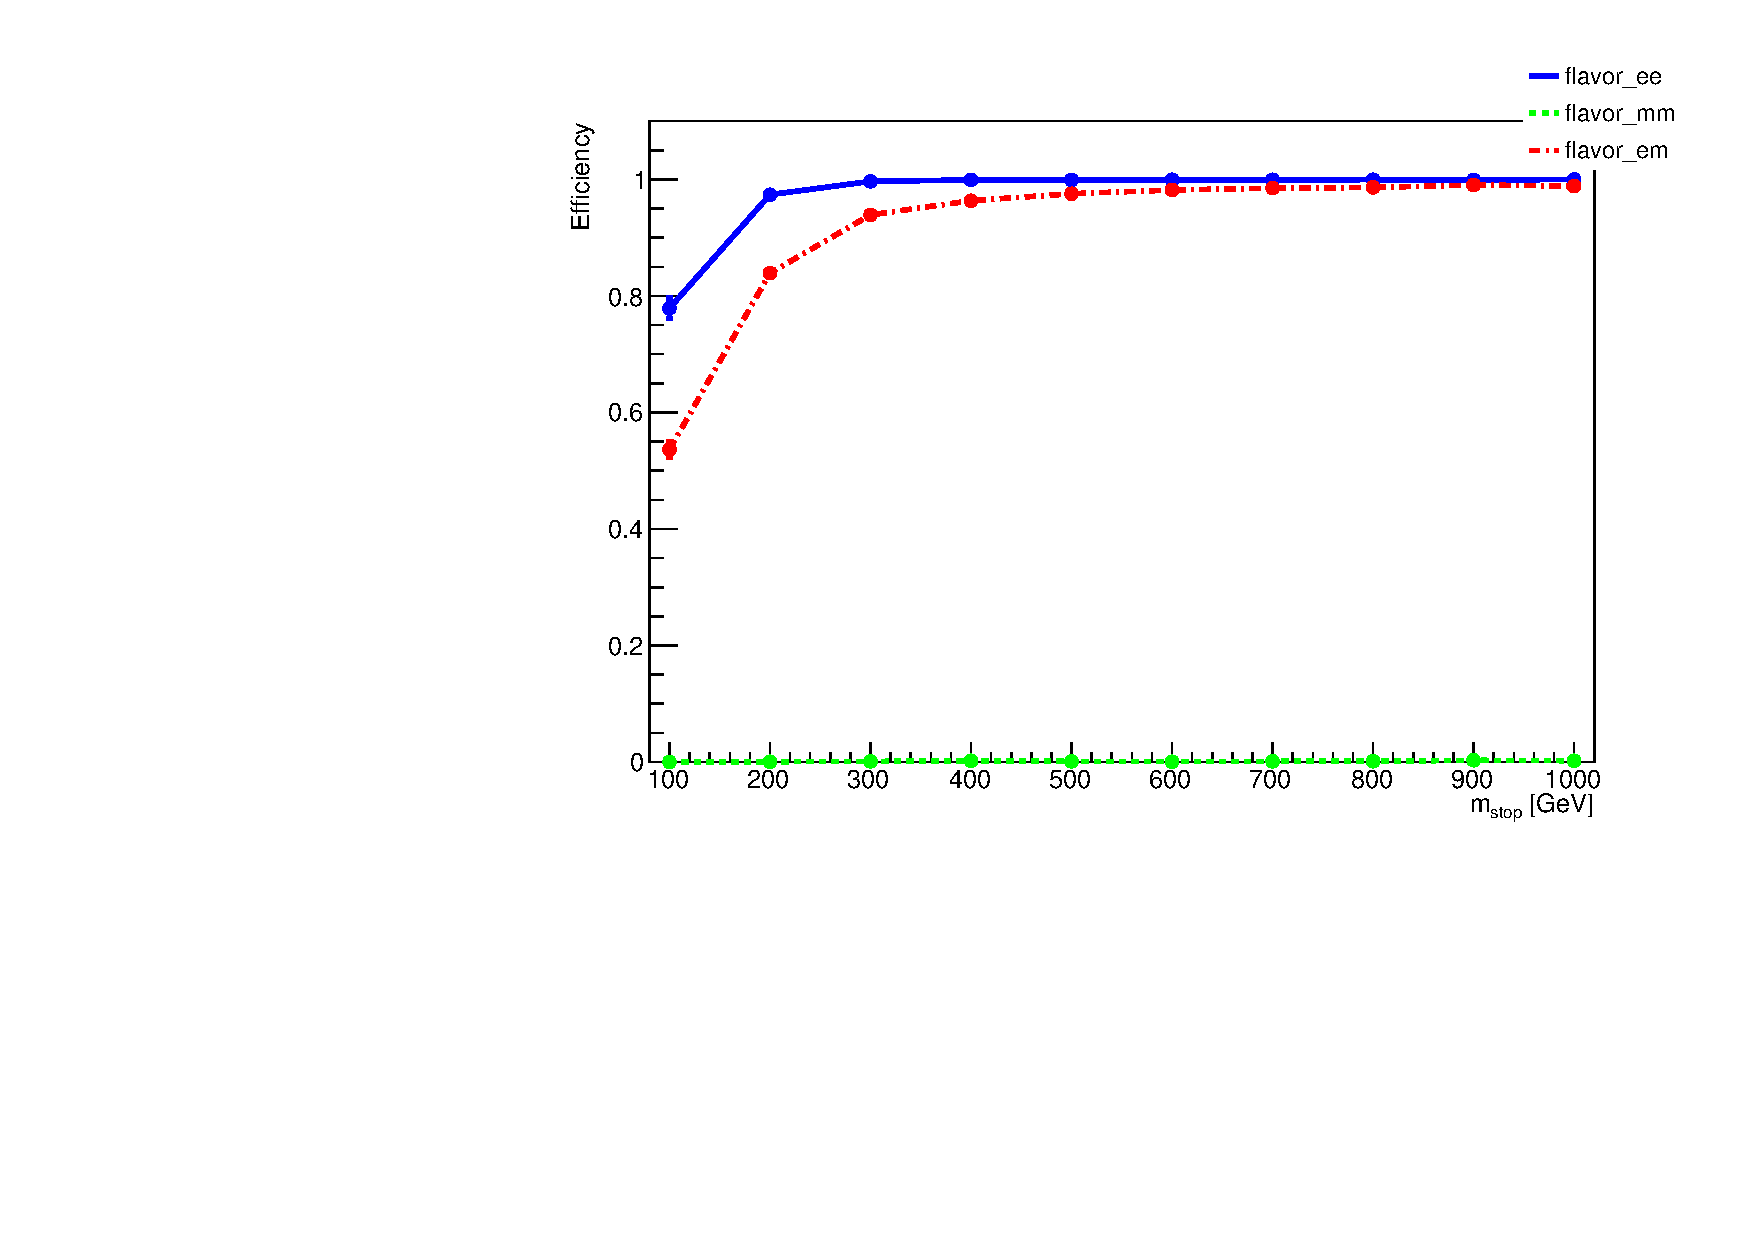
\includegraphics[width=0.48\textwidth]
      {figs/trigger/EF_e60_medium1.pdf}
  }
  \subbottom[\texttt{EF\_mu24i\_tight trigger}]{
    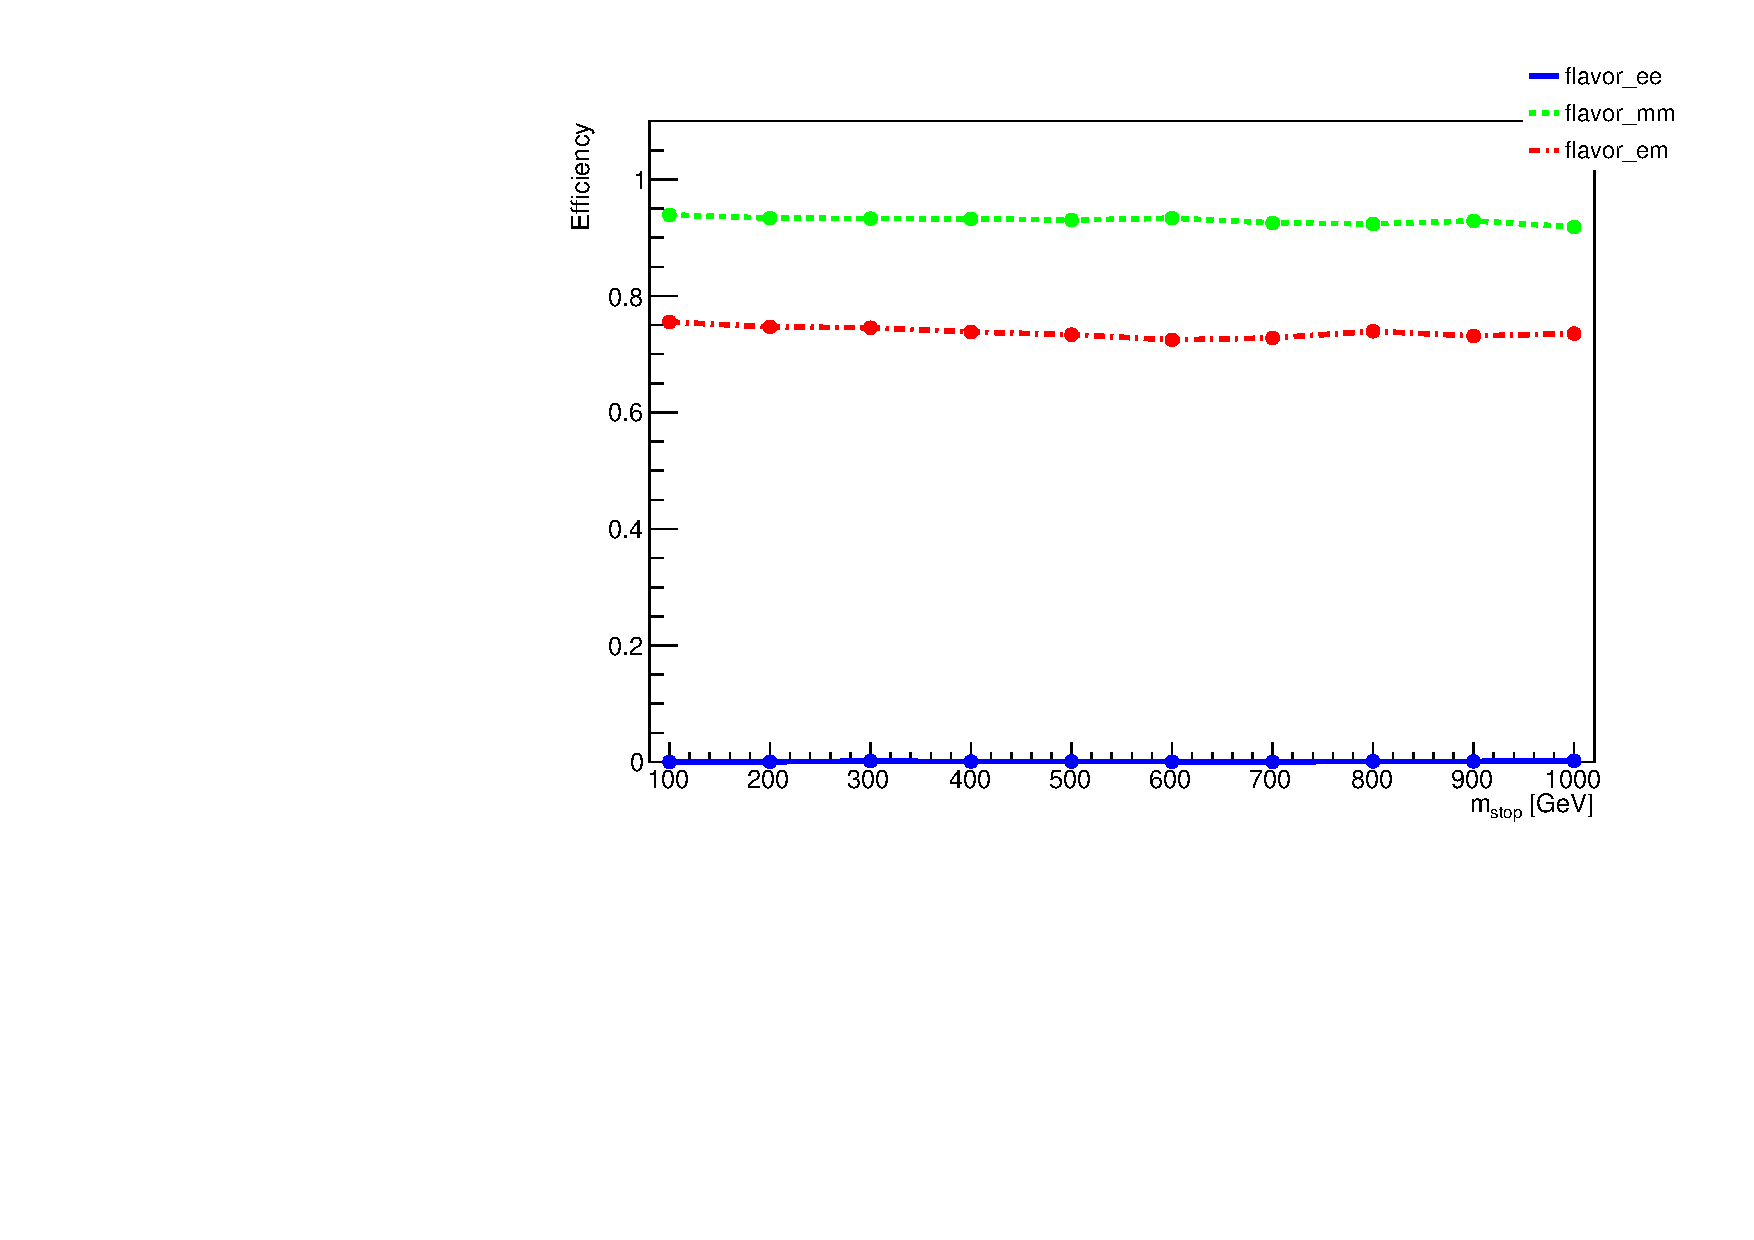
\includegraphics[width=0.48\textwidth]
      {figs/trigger/EF_mu24i_tight.pdf}
  }
  \subbottom[\texttt{EF\_mu36\_tight}]{
    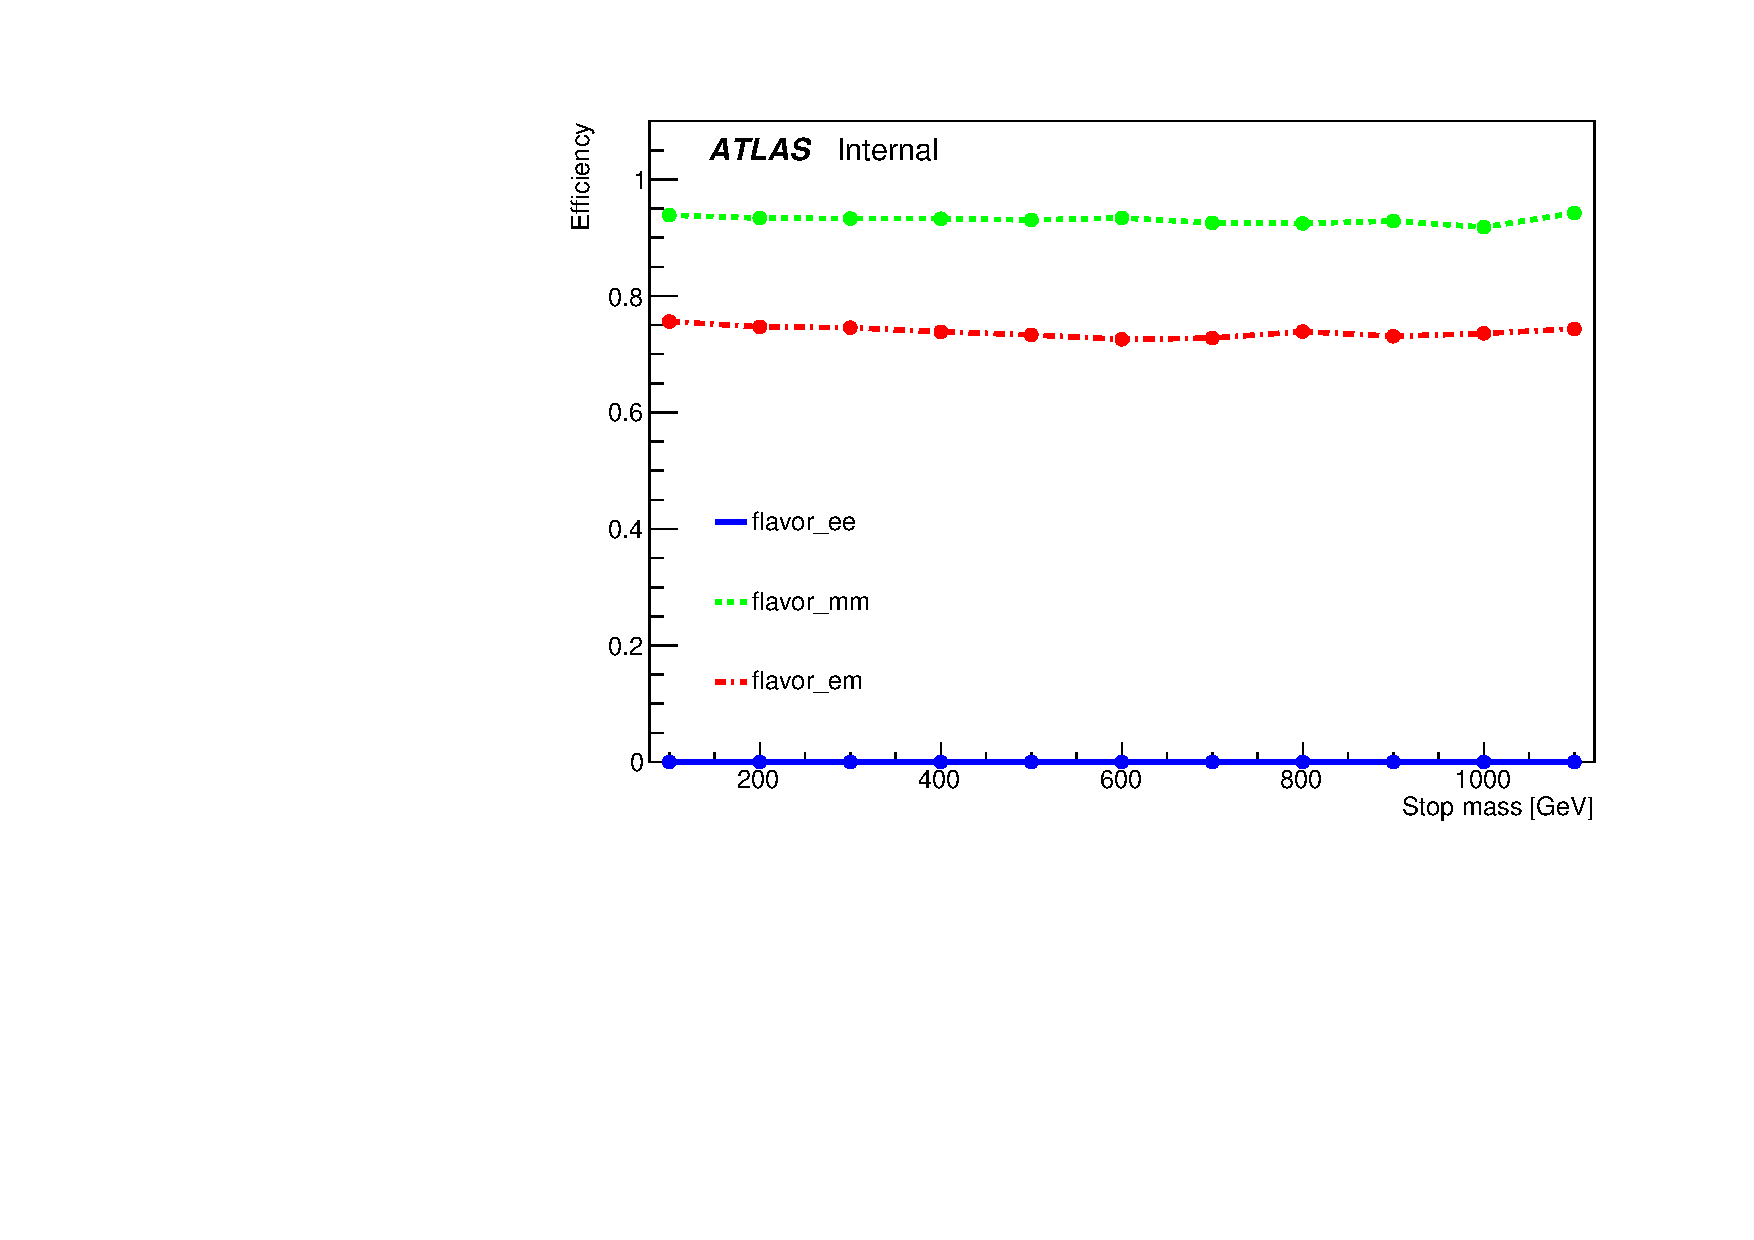
\includegraphics[width=0.48\textwidth]
      {figs/trigger/EF_mu36_tight.pdf}
  }
  \caption{Efficiency of simulated stop events passing each single lepton
    trigger broken down by flavor channel.
    The two single electron triggers have different shapes, which the 
    \texttt{EF\_e24vhi\_medium1} trigger being more efficient for low stop
    masses and the \texttt{EF\_e60\_medium1} trigger more efficient for
    higher stop masses.
    The two single muon triggers have roughly equal efficiency for all stop
    masses.
    Due to the trigger requirement, and the overlap removal procedure, $ee$
    events do not pass the single muon triggers, and $\mu\mu$ events do not
    pass the single electron triggers.
  }
  \label{fig:single_trigger_efficiency}
\end{figure}

\begin{figure}[ht]
  \centering
  \subbottom[\texttt{EF\_e24vhi\_medium1}]{
    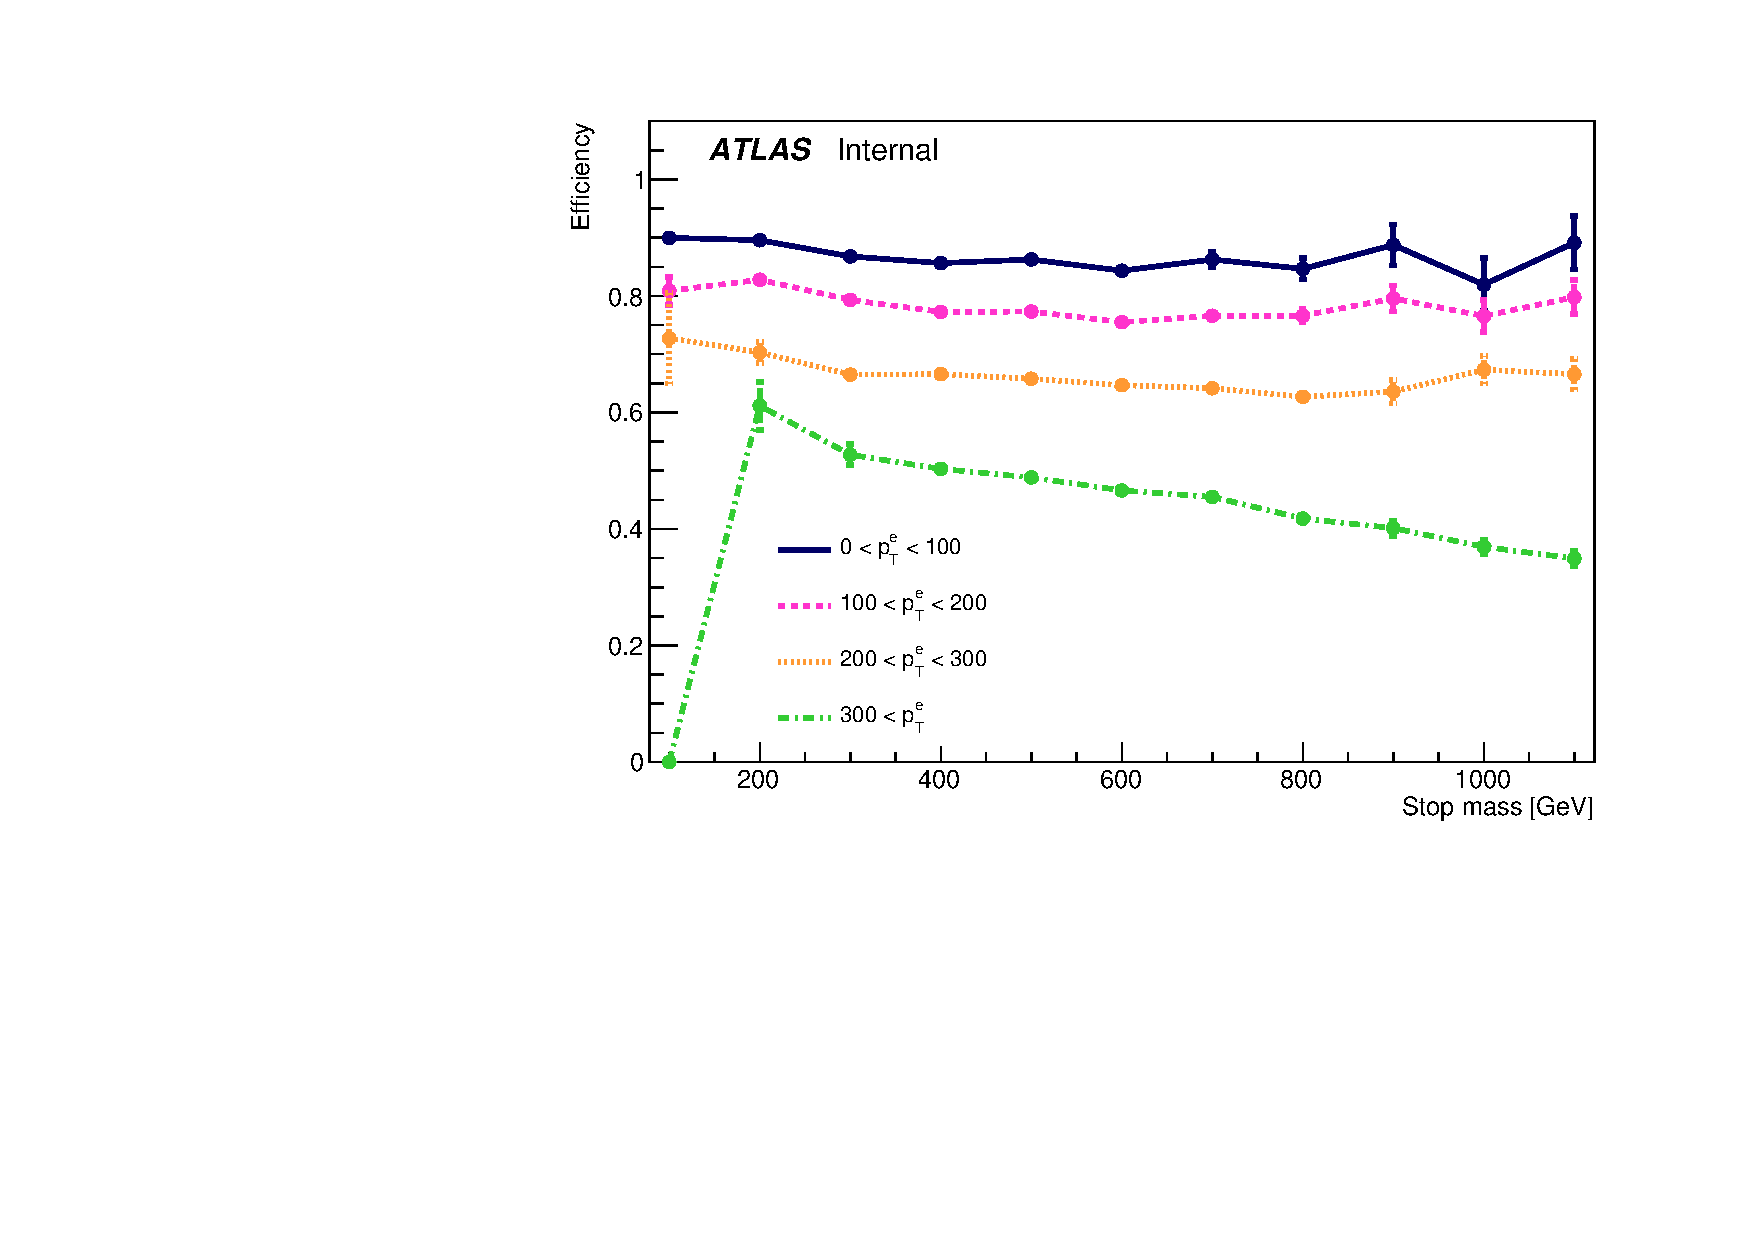
\includegraphics[width=0.48\textwidth, clip=true, trim=0 0 1cm 0]
      {figs/trigger/EF_e24vhi_medium1__el_pt.pdf}
  }
  \subbottom[\texttt{EF\_e60\_medium1}]{
    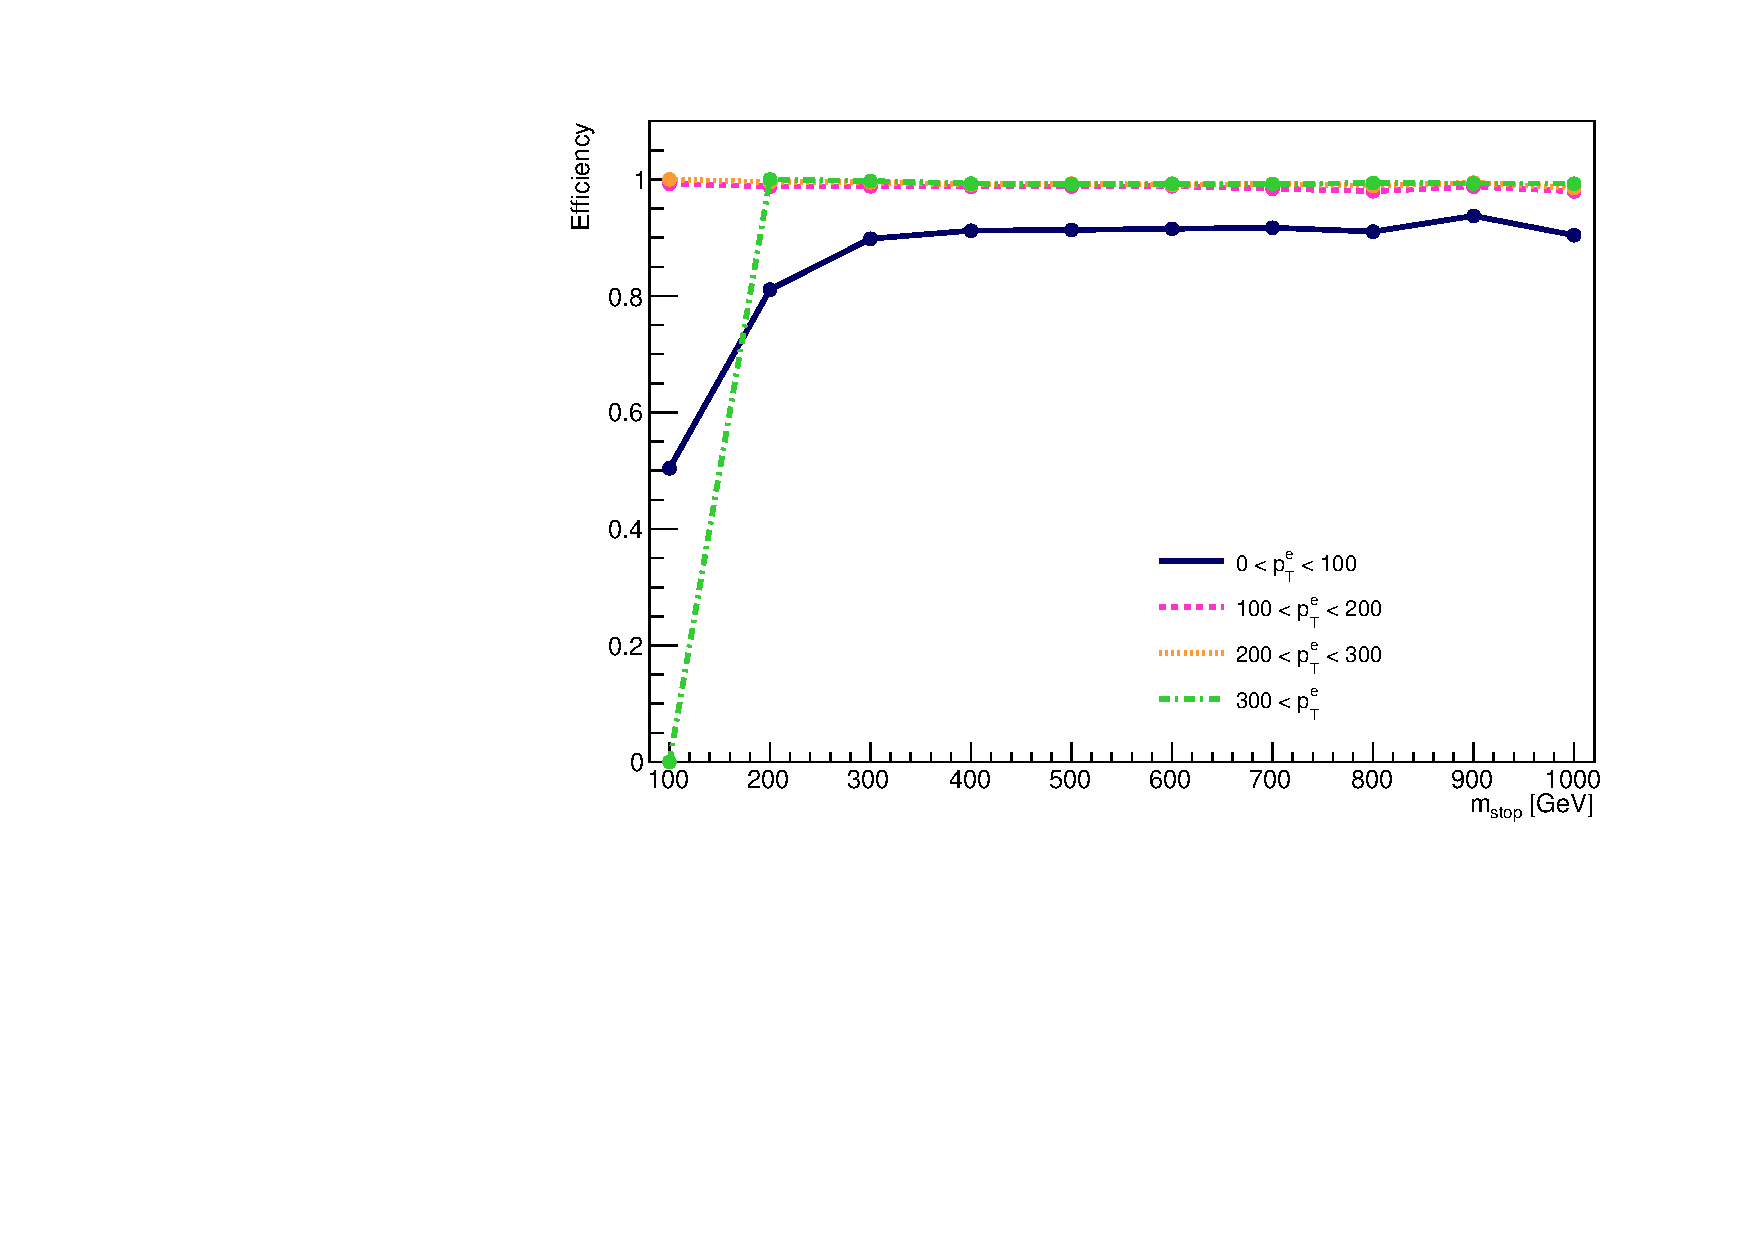
\includegraphics[width=0.48\textwidth, clip=true, trim=0 0 1cm 0]
      {figs/trigger/EF_e60_medium1__el_pt.pdf}
  }
  \caption{Efficiency of simulated stop events passing each of the single
    electron triggers for several ranges of electron \ET.
    Only $e\mu$ events are shown in order to show to isolate the effect of
    the electron \ET\ on the single electron trigger efficiency.
    These plots show the trigger efficiency dependence on the stop mass,
    observed in Figure~\ref{fig:single_trigger_efficiency} is due to a
    dependence on the electron \HT.
    The \texttt{EF\_e24vhi\_medium1} trigger has the high efficiency for low
    \HT\ electrons, while the \texttt{EF\_e60\_medium1} trigger is more
    efficient for high \HT\ electrons.
  }
  \label{fig:electron_trigger_pt_dependence}
\end{figure}

The full trigger requirement is highly efficient for signal-like events; between
93\% and 98\% of simulated signal events pass the trigger selection depending
on the flavor channel as shown in Figure~\ref{fig:full_trigger_efficiency}.

\begin{figure}[ht]
  \centering
  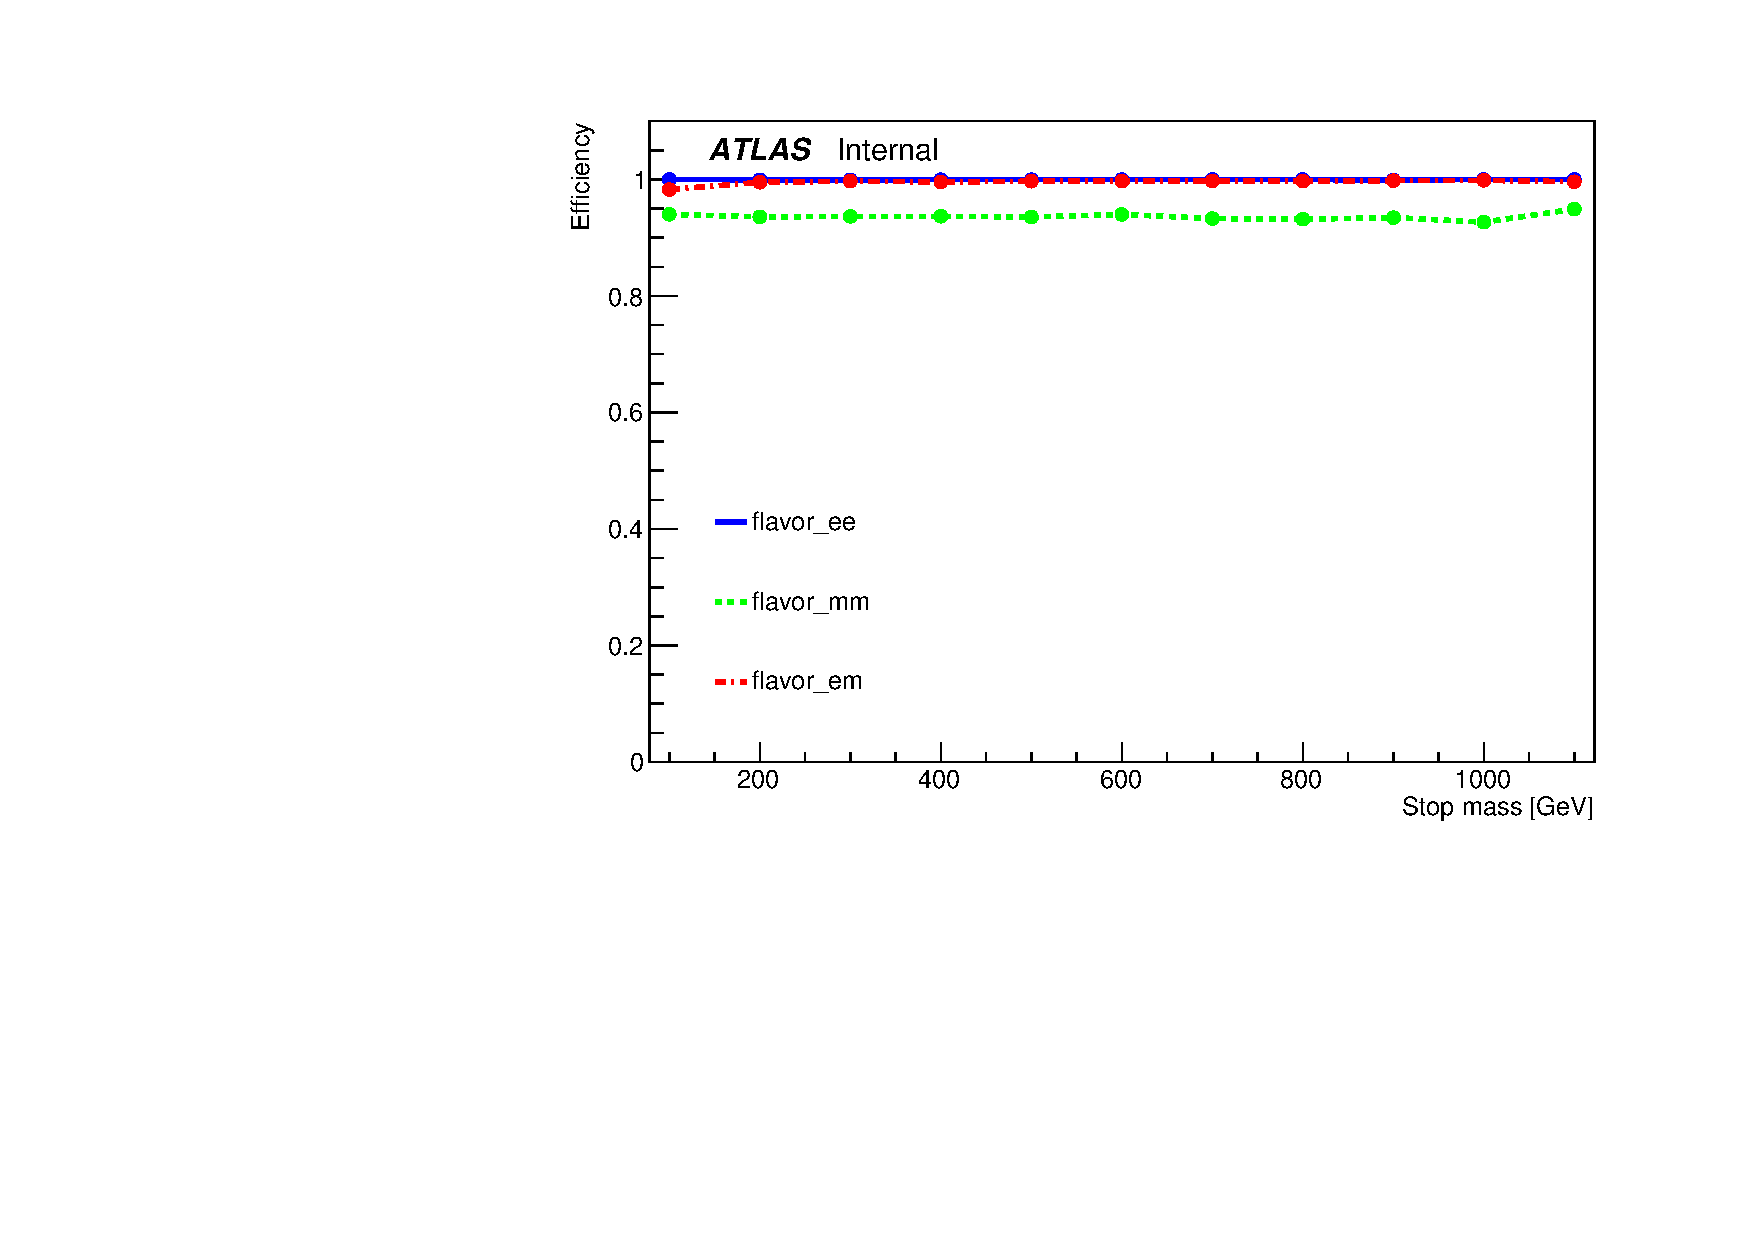
\includegraphics[width=0.60\textwidth]
    {figs/trigger/EF_e24vhi_medium1_OR_EF_e60_medium1_OR_EF_mu24i_tight_OR_EF_mu36_tight.pdf}
  \caption{Efficiency of simulated stop events passing the full trigger
    selection broken down by flavor channel.
    When the full trigger selection is considered, the trigger efficiency does
    not depend on the stop mass.
  }
  \label{fig:full_trigger_efficiency}
\end{figure}

The trigger requirement is applied in both data and MC simulation.
To account for the difference in trigger efficiency, a trigger scale factor is
applied to the MC events which passed the trigger requirement.
The trigger efficiencies for data and MC simulation are provided by
the Egamma and Muon combined performance groups.
The trigger scale factor is the ratio of the efficiencies (data to MC
simulation) for an event passing the trigger requirement, as described in
Table~\ref{tab:triggers}, and is given by
\begin{equation}
  SF_\mathrm{trigger} =
  \frac{1- \prod_{t \in \mathrm{triggers}}\prod_{\ell \in \{0,1\}}
                 (1-\epsilon_{\ell, t}^\mathrm{data})}
       {1- \prod_{t \in \mathrm{triggers}}\prod_{\ell \in \{0,1\}}
                 (1-\epsilon_{\ell, t}^\mathrm{MC})},
\end{equation}
where $\epsilon_{\ell,t}^\mathrm{data}$ ($\epsilon_{\ell,t}^\mathrm{MC}$) is
the trigger efficiency (electron or muon) for lepton $\ell$ to pass trigger $t$
in the data (MC simulation).
The trigger scale factor is calculated using only the two signal leptons in the
event, and they are the only objects considered when checking the trigger
requirement.
The efficiency for an electron (muon) to pass one of the muon (electron)
triggers is set to zero.
This is justified based on the trigger efficiencies shown in
Figure~\ref{fig:single_trigger_efficiency}.
The trigger scale factor is treated as an additional event weight for events in
the MC simulation.

%% -----------------------------------------------------------------------------
\FloatBarrier
\section{Signal regions}
\label{sec:signal_regions}

This analysis targets a wide range of stop masses, which differ greatly in the
expected cross sections and the expected event kinematics.
For this reason, two overlapping signal regions (SRs) are defined to search for
an excess of signal-like events, which are inconsistent with the prediction from
the SM alone.
The two signal regions target the low stop mass and high stop mass regions
separately.

One of the major sources of SM background come from \ZGAMMAJETS.
To reduce this background, events where the two leptons have the same
flavor, and reconstruct an invariant mass consistent with the mass of the $Z$
boson ($|m_{\ell\ell} - m_{Z}| \leq 10 \GeV$) are rejected.

The scalar sum of the \pt\ of the two $b$-tagged jets and two leptons (\HT) 
effectively separates the signal processes from the major sources of
Standard Model background.
The stops of interest are extremely massive, so all the decay products tend to
have a large amount of energy, resulting in a high \HT.
SM processes, such as \TTBAR\ and \ZGAMMAJETS, do not have as large \HT.

For the signal model, the two $b\ell$ pairs making up the final state are the
decay products of the stop/anti-stop, and therefore have the same mass.
The mass asymmetry variable is defined as
\begin{equation}
  \MBLASYM = 
  \frac{\MBL^0-\MBL^1}{\MBL^0+\MBL^1}.
\end{equation}
Events from stop decays are expected to have low \MBLASYM\ as the mass
difference in the two pairs is expected to be small, while the masses of the
$b\ell$ pairs coming from SM processes are roughly uncorrelated, and there is
no preference for \MBLASYM.
The asymmetry is used rather than the simple difference in the masses so a
single cut value can be used for all stop masses which are considered.
Furthermore, events from SM background processes tend to have low \MBL\ for
both pairs.
The $\MBL^0$ variable can also provide additional discrimination power.
The expected \MLL, \HT, \MBLASYM\, and $\MBL^{0}$ distributions for SM
background processes and three signal models is shown in an inclusive region
after event cleaning and selecting two $b$-tagged jets and two leptons in
Figure~\ref{fig:no_data__no_k__inclusive_flavor_all__kinematic_dists}.

\begin{figure}
  \centering
  \subbottom[\MLL]{
    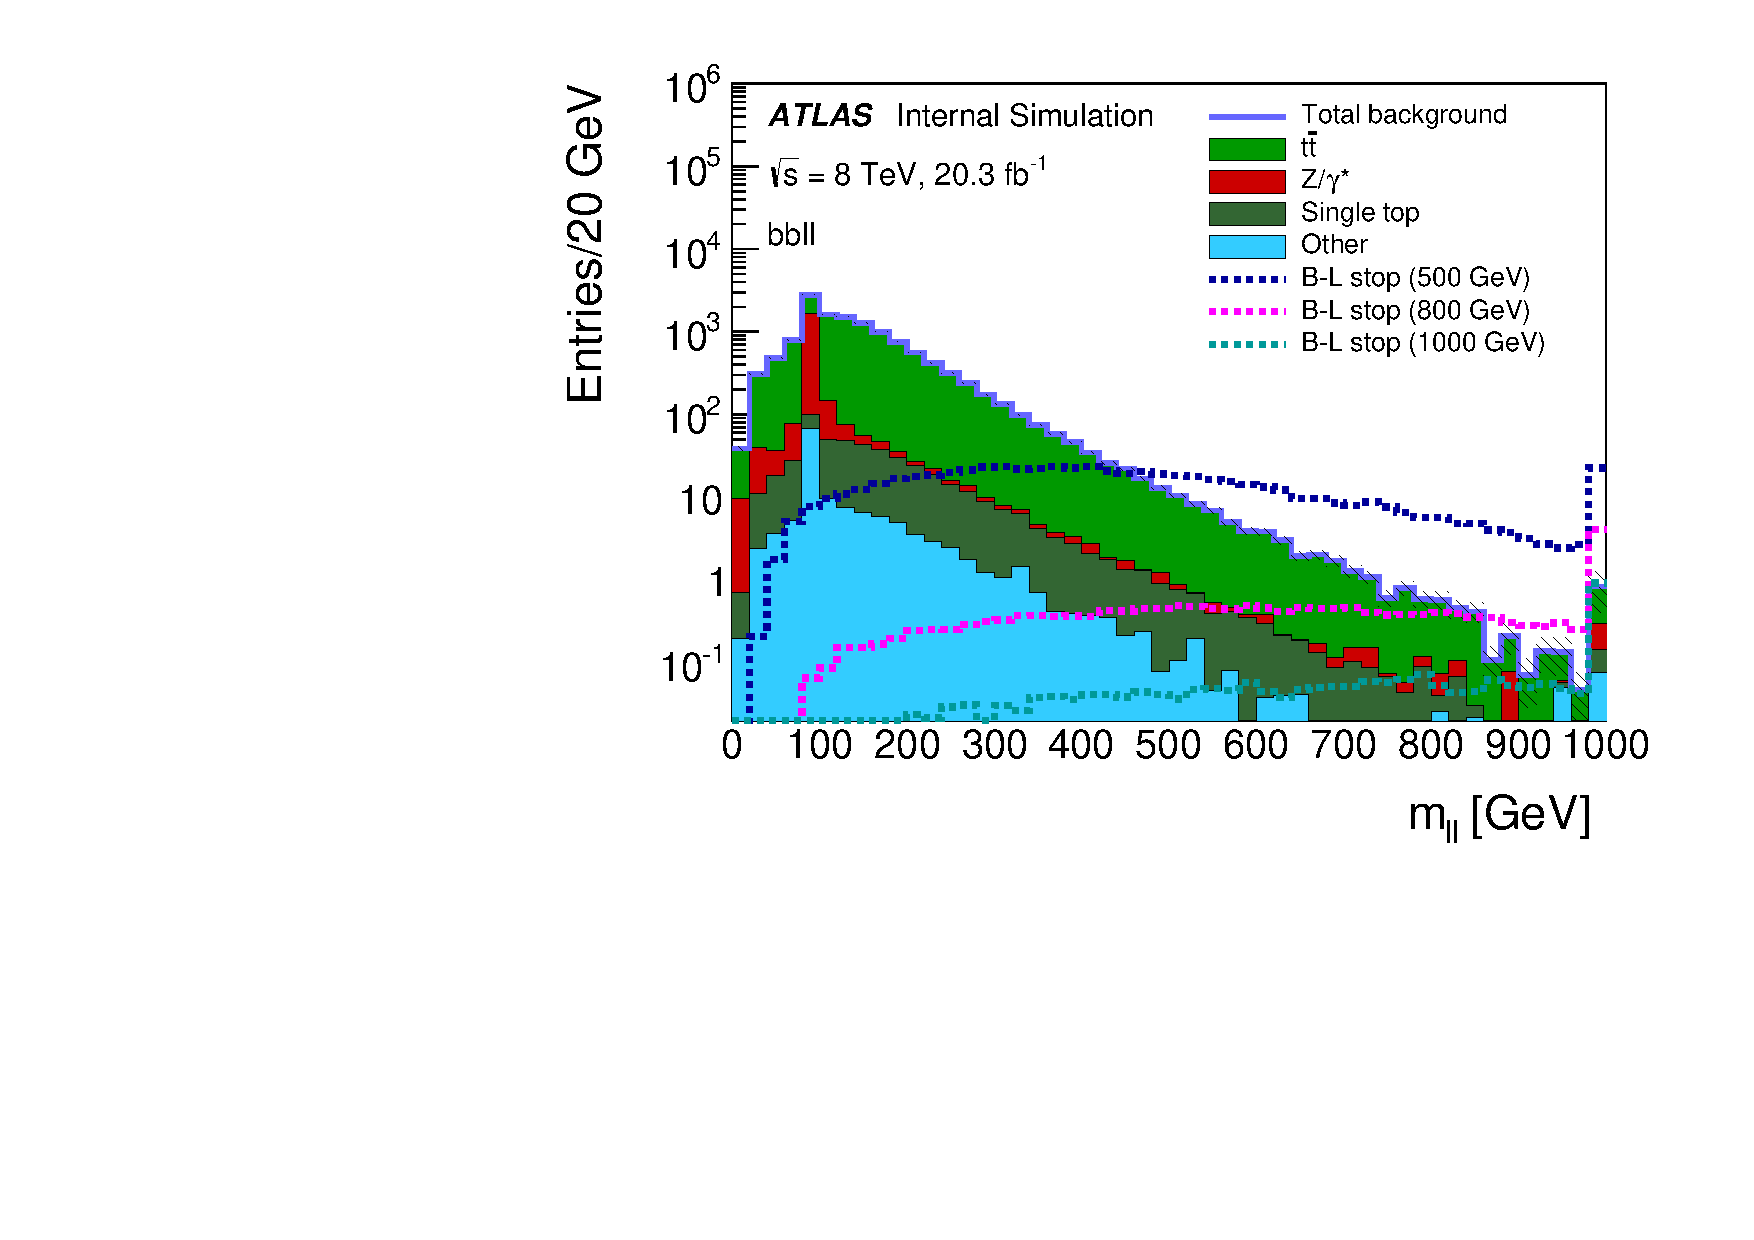
\includegraphics[width=0.48\textwidth, clip=true, trim=0 0 1cm 0]
    {figs/blstop/no_data__no_k_factor__dists/flavor_all__mll__BMINUSL_BL_PAIRING__log.pdf}
  }
  \subbottom[\HT]{
    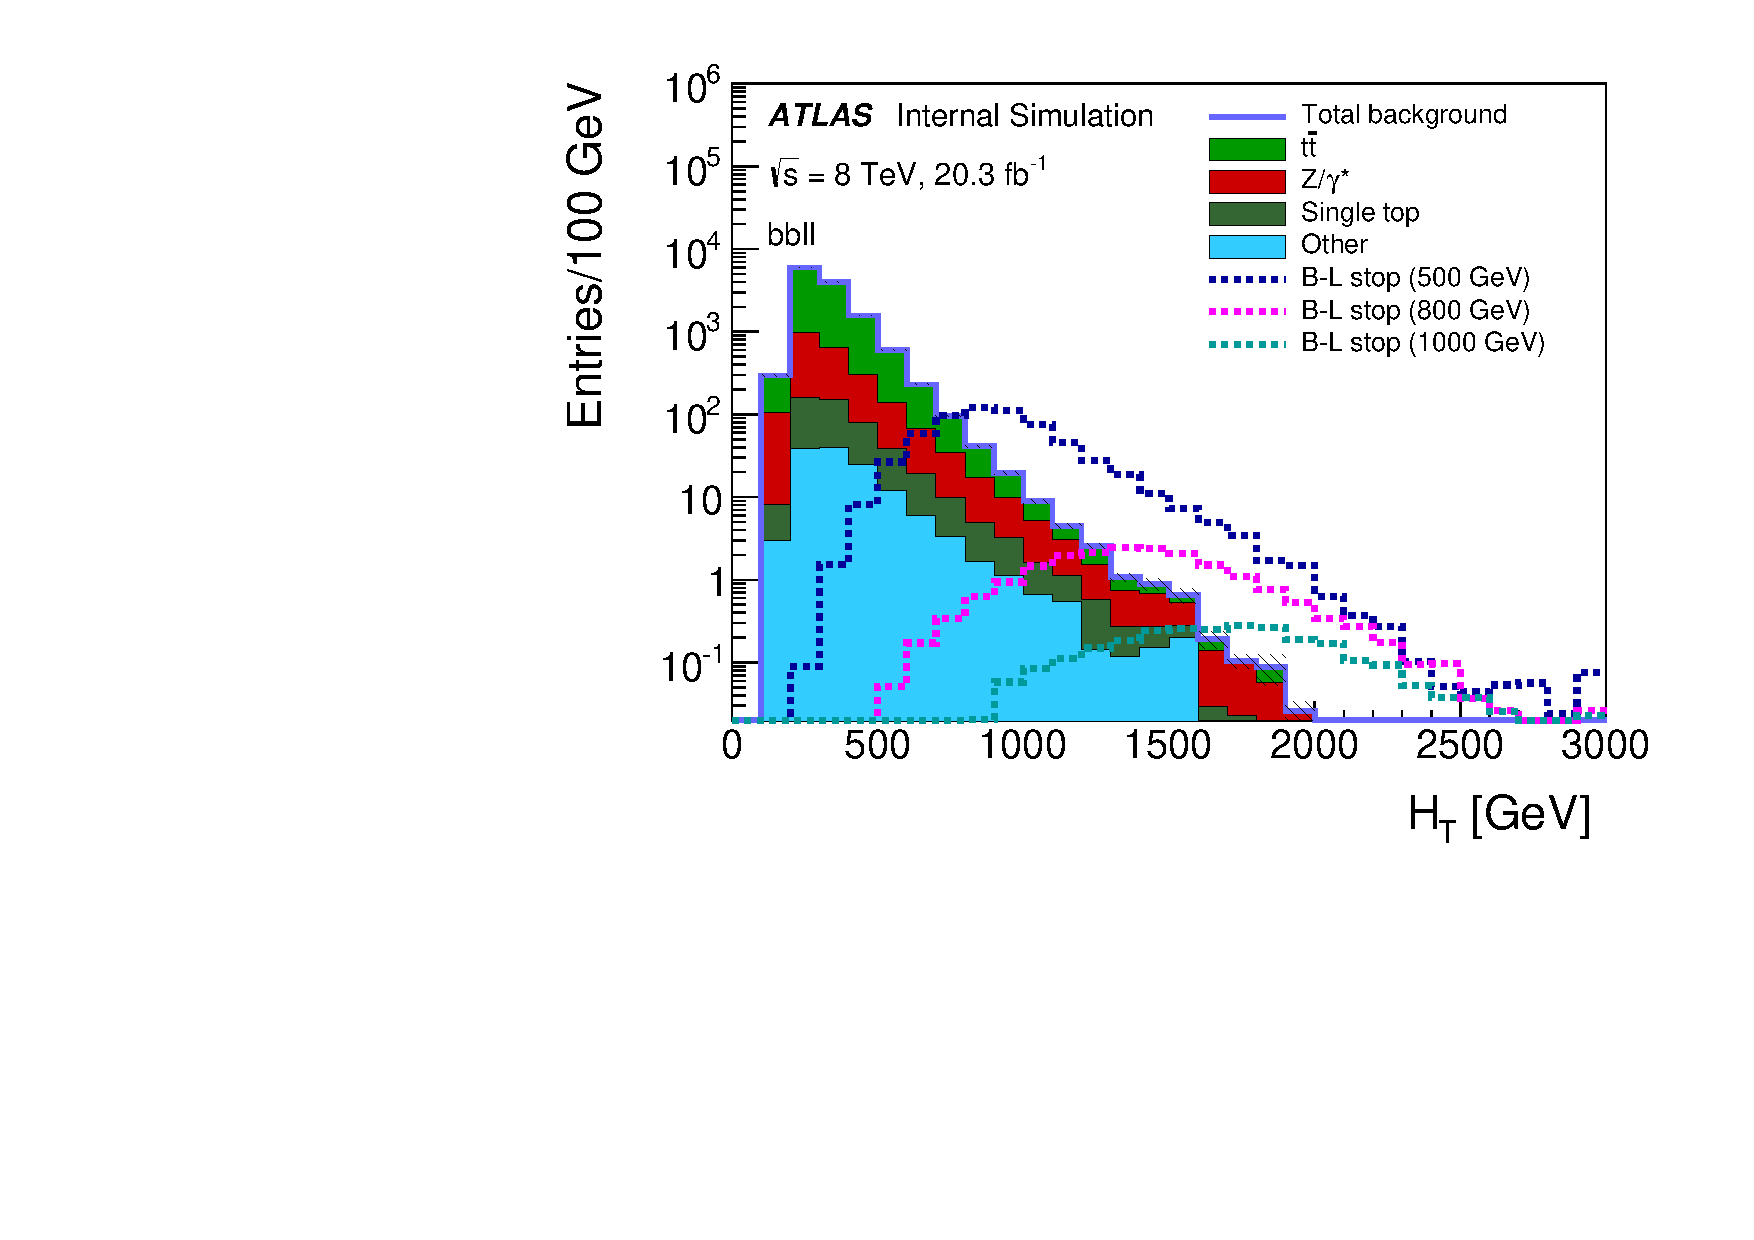
\includegraphics[width=0.48\textwidth, clip=true, trim=0 0 1cm 0]
    {figs/blstop/no_data__no_k_factor__dists/flavor_all__ht_signal__BMINUSL_BL_PAIRING__log.pdf}
  }
  \subbottom[\MBLASYM]{
    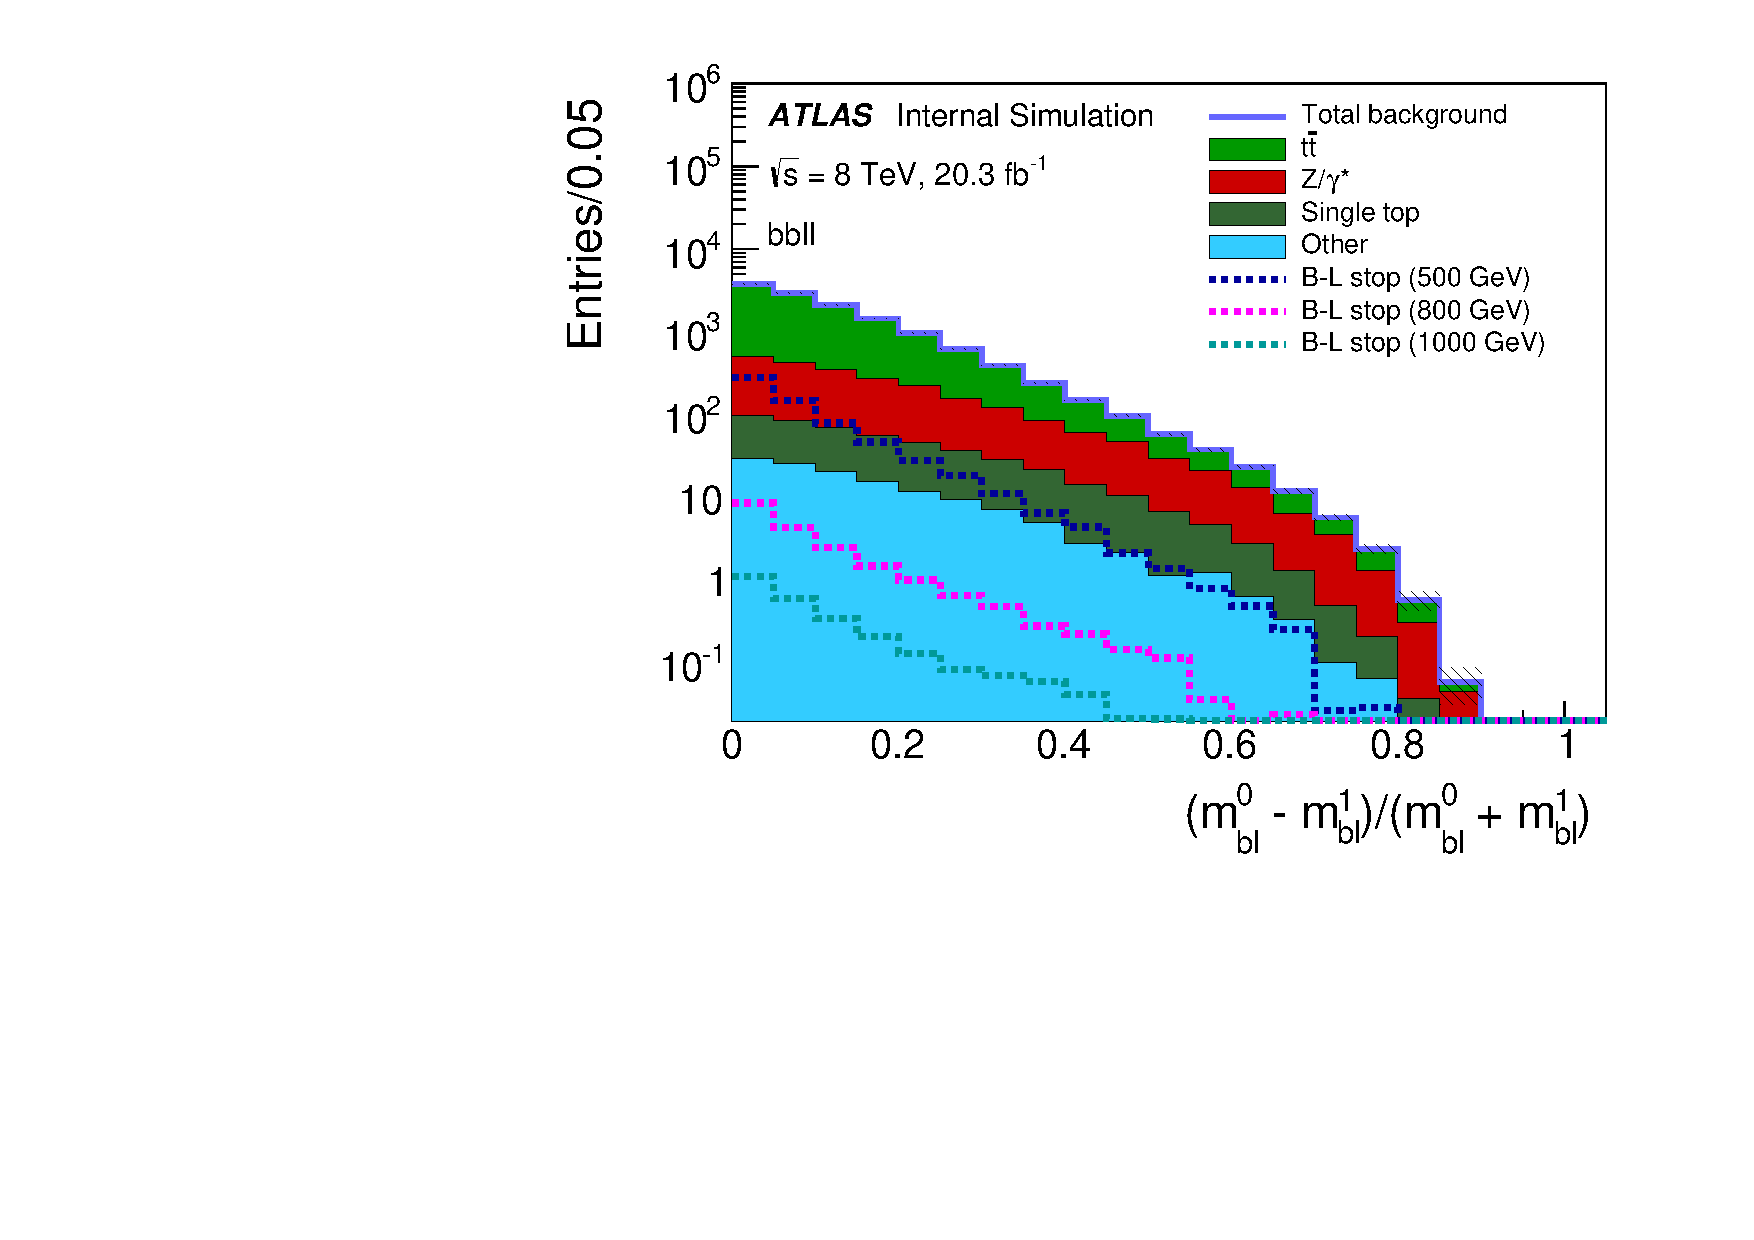
\includegraphics[width=0.48\textwidth, clip=true, trim=0 0 1cm 0]
    {figs/blstop/no_data__no_k_factor__dists/flavor_all__mbl_asym__BMINUSL_BL_PAIRING__log.pdf}
  }
  \subbottom[$\MBL^0$]{
    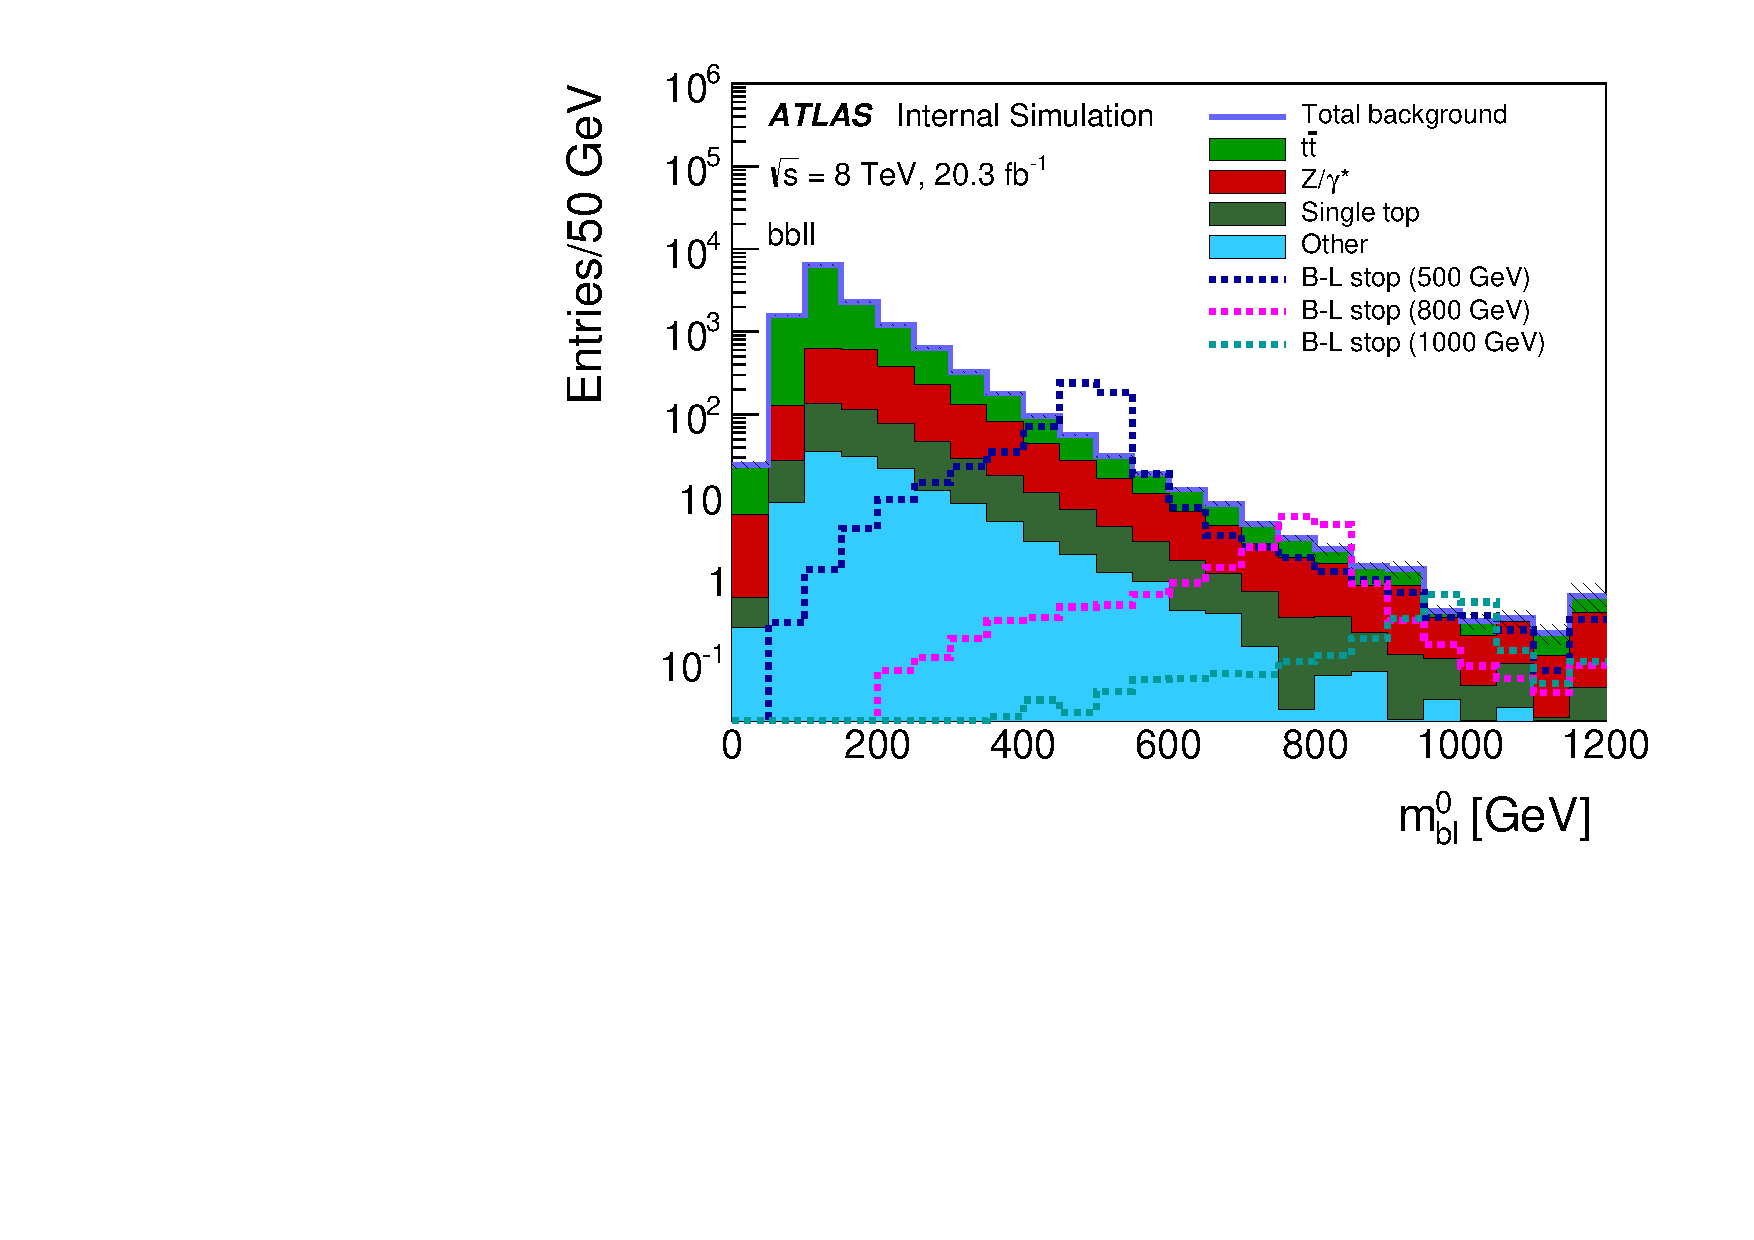
\includegraphics[width=0.48\textwidth, clip=true, trim=0 0 1cm 0]
    {figs/blstop/no_data__no_k_factor__dists/flavor_all__mbl_0__BMINUSL_BL_PAIRING__log.pdf}
  }
  \caption{Expected \MLL, \HT, \MBLASYM, and $\MBL^0$ distributions for SM
    background processes and three simulated stop samples with different masses.
    Basic event cleaning is applied and the events are required to pass the
    trigger selection, as described in
    Sections~\ref{sec:event_cleaning}~and~\ref{sec:trigger_selection}, and the
    events are required to have at least two $b$-tagged jets and two light
    leptons (electrons or muons).
    In each plot, the last bin includes the overflow for values beyond the
    maximum shown. The hashed error bands show only the statistical
    uncertainty on the background MC simulation samples. The signal
    models have an assumed
    $Br(\STOP\rightarrow~be)~=~Br(\STOP\rightarrow~b\mu)~=~0.5$.
  }
  \label{fig:no_data__no_k__inclusive_flavor_all__kinematic_dists}
  %%
\end{figure}

In order to achieve a large expected signal to background ratio in the signal
regions, MC simulation is used to optimize the selection requirements.
The optimization is performed assuming a stop branching fraction of
$Br(\STOP\rightarrow~be)~=~Br(\STOP\rightarrow~b\mu)~=~0.5$.
A single SR selection criteria is obtained for both the \HT\ and
\MBLASYM\ variables which perform reasonably well for all mass above 500 \GeV.
Events in both SRs are required to have $\HT \geq 1100~\GeV$ and
$\MBLASYM \leq 0.2$.
$\MBL^0$ is used to define the two SRs.
SR~400 has a requirement of $\MBL^0 \geq 400 \GeV$, and is optimal for lower
stop masses, while SR~600, with a requirement of $\MBL^0 \geq 600 \GeV$, is
optimal for higher stop masses.

Events in the SRs are required to have \HT\ above 1100~\GeV.
Events with two same-flavor leptons with invariant mass within 10~\GeV\ of the
$Z$-boson mass are vetoed to reduce the backgrounds from $Z$-boson production.
The SRs require a mass asymmetry of less than or equal to 0.2.
Finally, $\MBL^0$ is used to define the two SRs.
SR~400 has a requirement of $\MBL^0 \geq 400 \GeV$, and is optimal for lower
stop masses, while SR~600 has a requirement of $\MBL^0 \geq 600 \GeV$, and is
optimal for higher stop masses.
Two additional SRs were considered with $\MBL^0 \geq 200 \GeV$ and
$\MBL^0 \geq 800 \GeV$ (SR~200 and SR~800 respectively), however these were
dropped from the analysis.
The SR~200 region did not provide additional expected sensitivity compared with
the SR~400 region, and the statistical uncertainty in the SR~800 region was very
large, and reduced expected sensitivity.
The full selection criteria for the analysis regions, including the Control and
Validation regions, described in Section~\ref{sec:bkg}, is outlined in
Table~\ref{tab:regions} and Figure~\ref{fig:region_coverage}.

%% - - - - - - - - - - - - - - - - - - - - - - - - - - - - - - - - - - - - - - -
\begin{table}[ht]
  \caption{Summary of signal, control, and validation regions used for this
    analysis.
    The control and validation regions are explained in Section~\ref{sec:bkg}.
    All regions require two $b$-tagged jets and two oppositely charged leptons.
    An event is in the $Z$ window if it contains two same-flavored leptons with
    an invariant mass within 10~\GeV\ of the mass of the $Z$ boson.
  }
  \label{tab:regions}
  %
  \centering{
    \begin{tabular}{l|ccccc}
      \toprule
      Region &
      $\MBL^0$ [\GeV] &
      \HT [\GeV] &
      \METSIG\ [$\GeV^{1/2}$] &
      \MBLASYM &
      $Z$ window \\
      \midrule
      SR~400   & $\geq 400$  & $\geq 1100$ & --       & $\leq 0.2$ & Veto   \\
      SR~600   & $\geq 600$  & $\geq 1100$ & --       & $\leq 0.2$ & Veto   \\
      \midrule
      Top CR   & $\geq 200$  & $\leq 500$  & $\geq 4$ & $\leq 0.2$ & Veto   \\
      $Z$ CR   & $\geq 200$  & $\leq 500$  & $\leq 4$ & $\leq 0.2$ & Select \\
      \midrule
      Top VR 1 & $\geq 200$  & $\leq 500$  & $< 4$    & $\leq 0.2$ & Veto   \\
      Top VR 2 & $\geq 200$  & $\leq 500$  & -        & $>    0.2$ & Veto   \\
      Top VR 3 & $\geq 200$  & $>   500$   & $> 4$    & $>    0.2$ & Veto   \\
      $Z$ VR   & $\geq 200$  & $>   500$   & --       & $\leq 0.2$ & Select \\
      \bottomrule
    \end{tabular}
  }
\end{table}

%% - - - - - - - - - - - - - - - - - - - - - - - - - - - - - - - - - - - - - - -
\begin{figure}[ht]
  \centering
  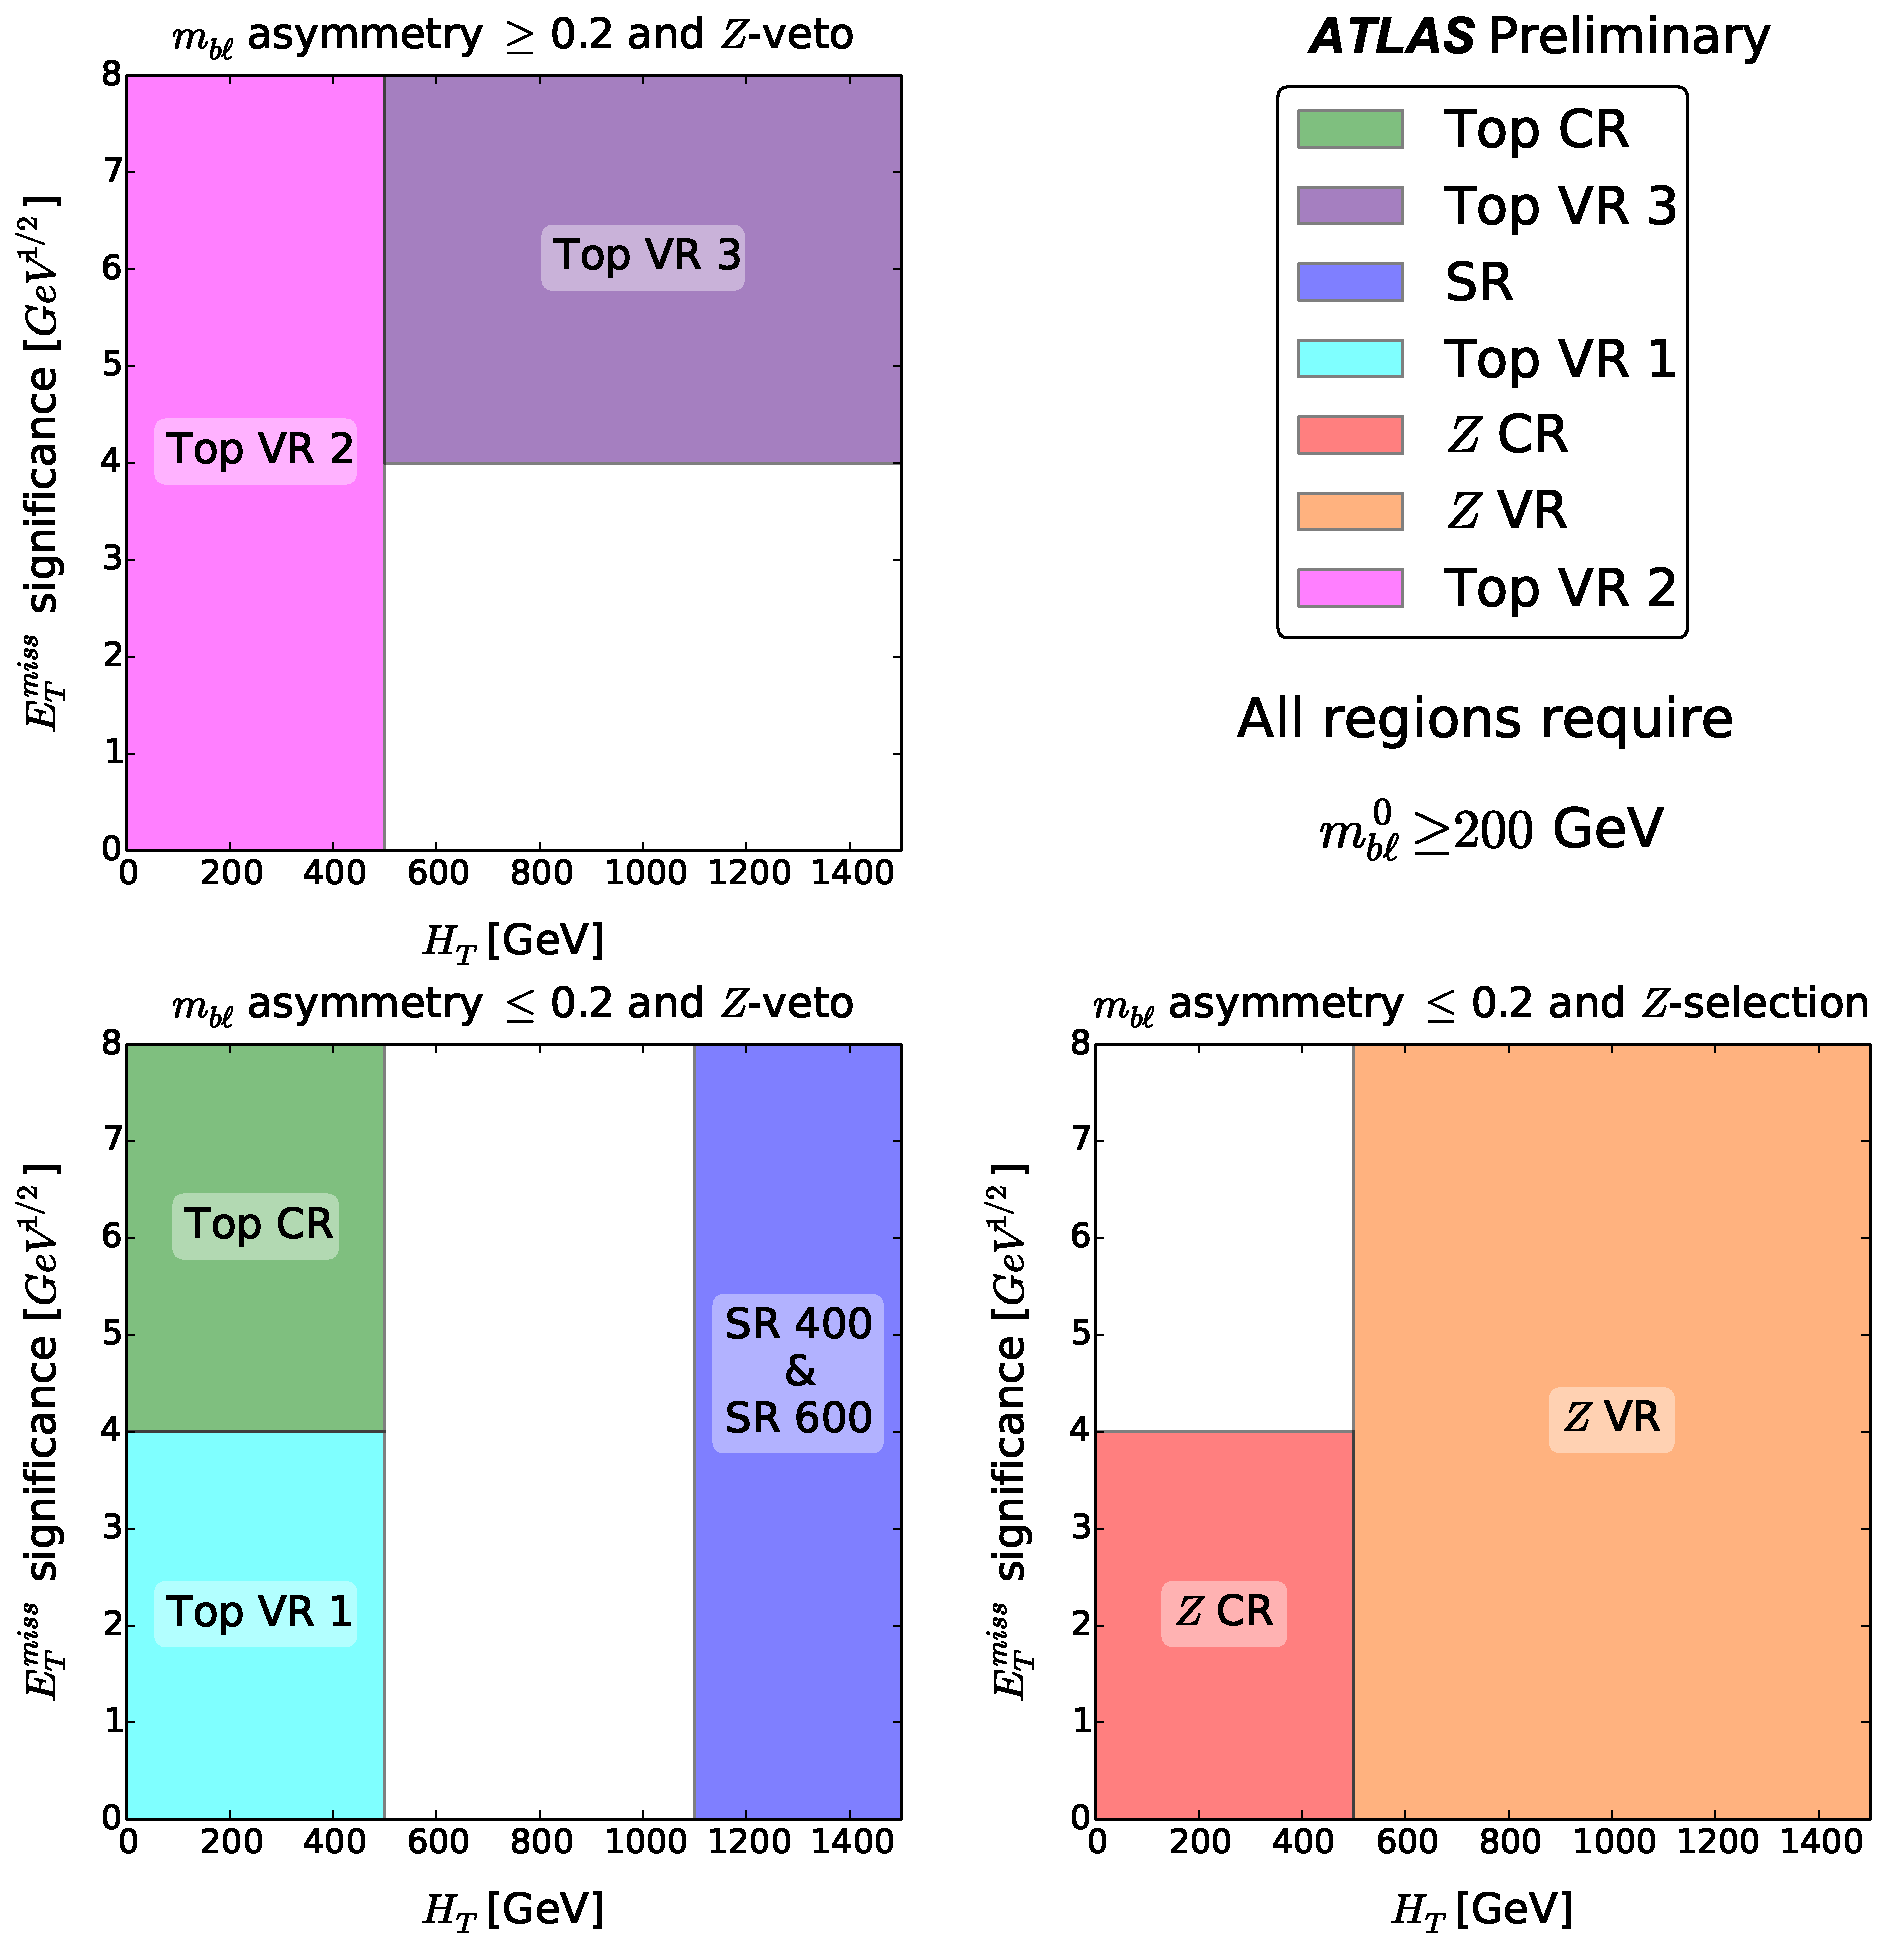
\includegraphics[width=\textwidth]{figs/blstop/regions__met_sig__ht_plane.pdf}
  \caption{Position of the regions in the \METSIG\ versus \HT\ space.
    The two left plots show the \METSIG-\HT~plane after vetoing events within
    the $Z$ window, with the top plot requiring $\MBLASYM \geq 0.2$ and the
    bottom requiring $\MBLASYM \leq 0.2$.
    The right plot shows the plane when requiring events be within the $Z$
    window.
    The two SRs apply a different requirement on the
    invariant mass of the higher-mass $b\ell$ pair. SR~400 requires
    $\MBL^{0} \geq 400 \GeV$, and SR~600 requires $\MBL^{0} \geq 600 \GeV$.
  }
  \label{fig:region_coverage}
\end{figure}

Figure~\ref{fig:n_minus_one_sr} shows the expected \HT, \MBLASYM, and $\MBL^0$
distributions after applying all the SR selection criteria except that on the
variable being shown.
This figure includes the simulated background processes and three signal models.
The number of expected signal events (for the same three signal models)
passing each selection requirement is shown in Table~\ref{tab:sr_cutflow}.
The estimates shown in Figure~\ref{fig:n_minus_one_sr} and
Table~\ref{tab:sr_cutflow} are taken from MC simulation, and the event
yields are normalized to 20.3 \ifb.

\begin{figure}
  \centering
  \subbottom[\HT]{
    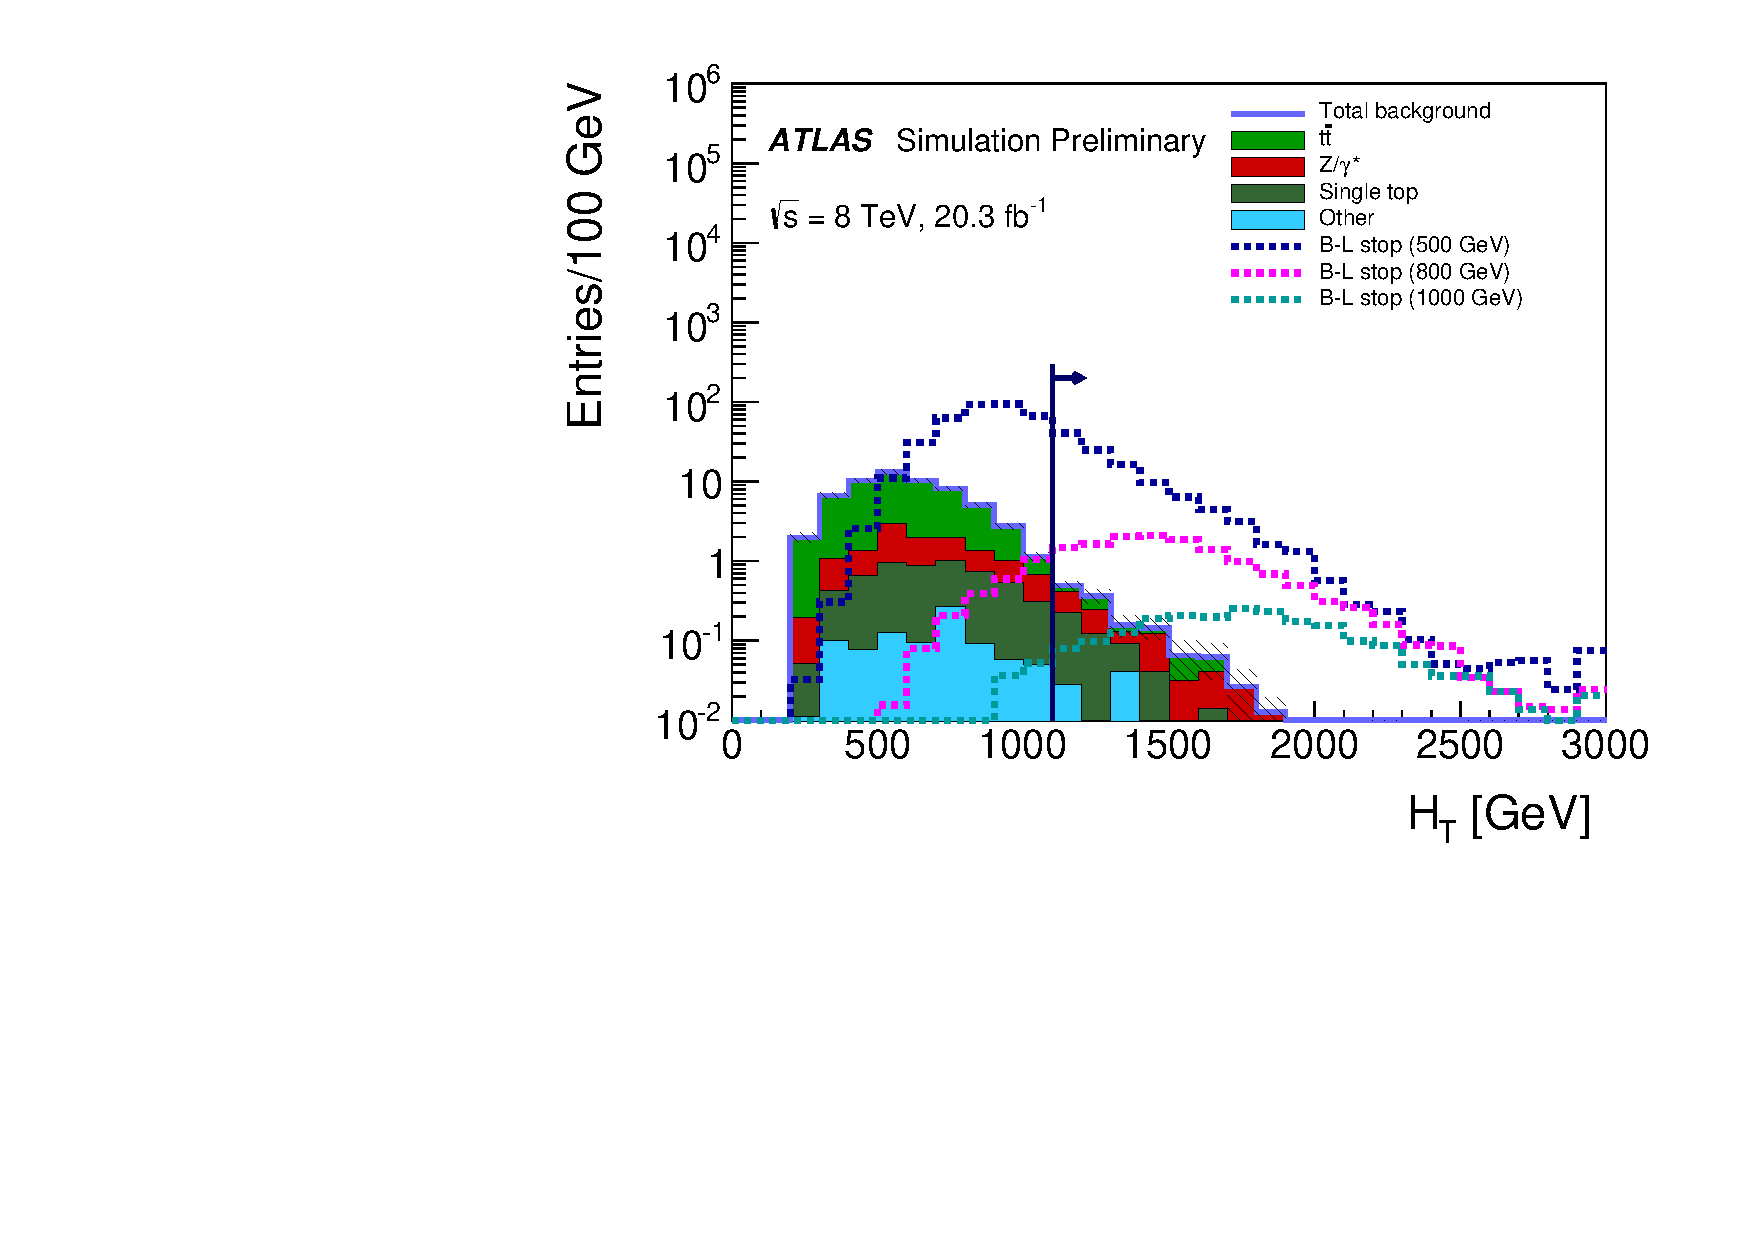
\includegraphics[width=0.48\textwidth, clip=true, trim=0 0 1cm 0]
      {figs/blstop/ht_sr_400_minus_ht.pdf}
  }
  \subbottom[\MBLASYM]{
    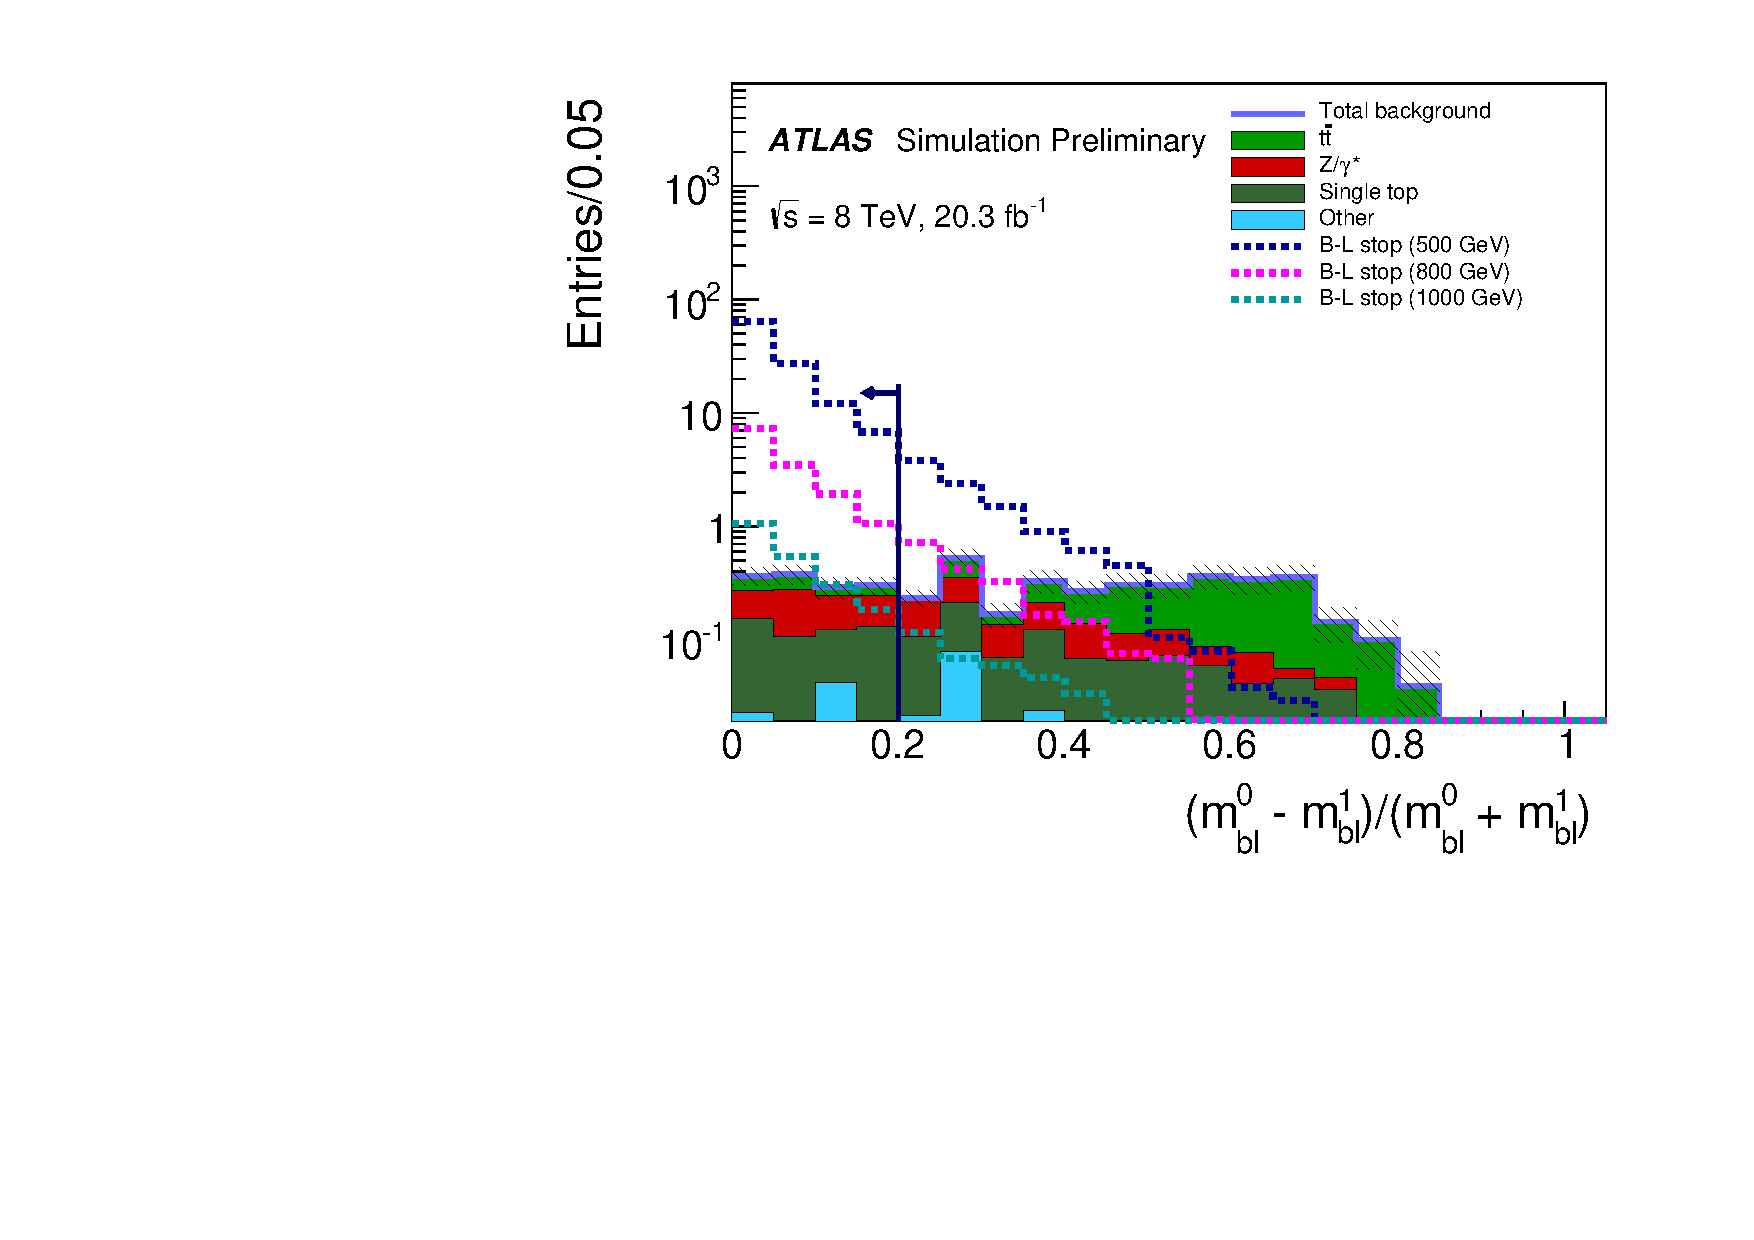
\includegraphics[width=0.48\textwidth, clip=true, trim=0 0 1cm 0]
      {figs/blstop/mbl_asym_sr_400_minus_mbl_asym.pdf}
  }
  \subbottom[$\MBL^0$]{
    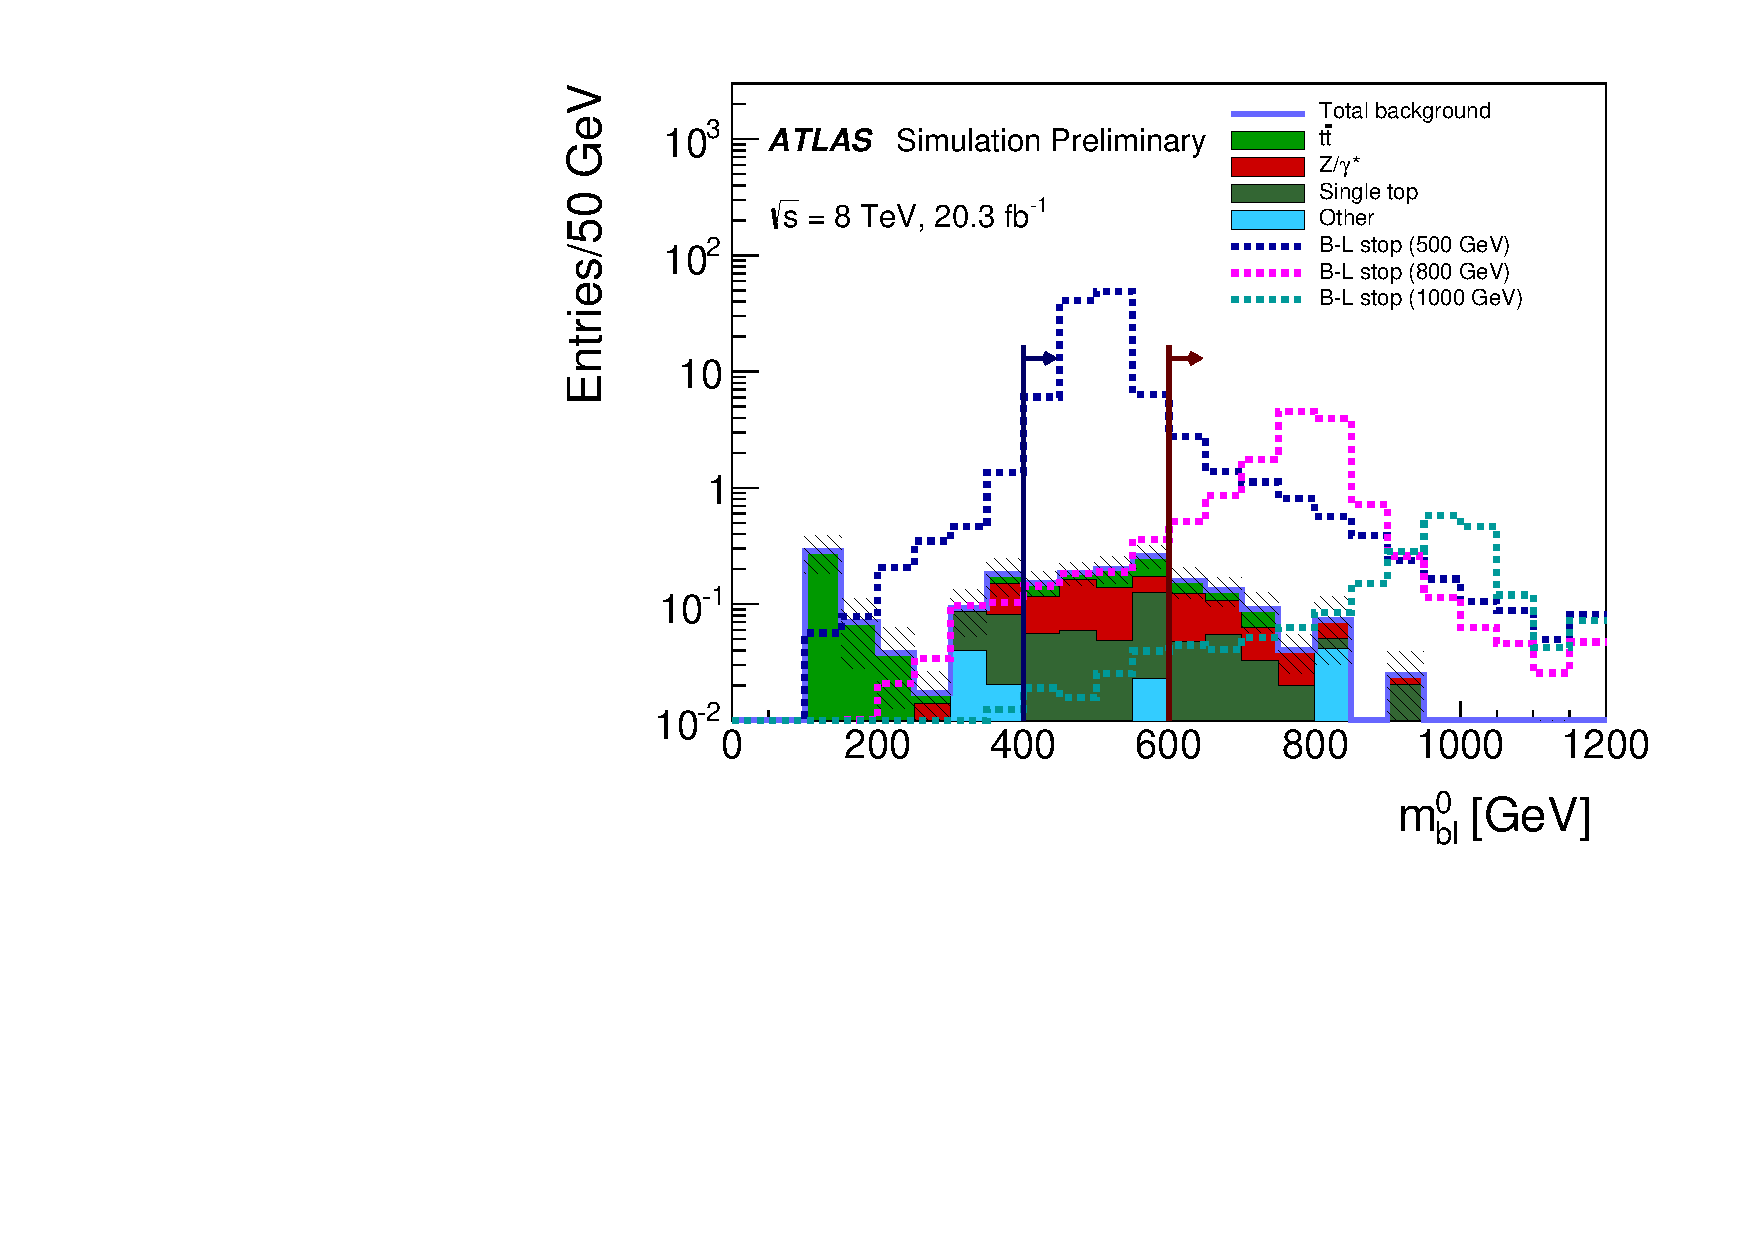
\includegraphics[width=0.48\textwidth, clip=true, trim=0 0 1cm 0]
      {figs/blstop/mbl_0_sr_minus_mbl.pdf}
  }
  \caption{Distributions of the variables which are used to define the SRs.
    These plots show the MC simulated background samples and three signal
    models, and are made after applying all the SR selection criteria except for
    that on the variable shown.
    The top two plots show the \HT\ and \MBLASYM\ variables, and the bottom
    plot shows the $\MBL^0$ distribution.
    The arrows show the SR requirement on the variable being shown.
    In each plot, the last bin includes the overflow for values beyond the
    maximum shown.
    The hashed error bands show only the statistical uncertainty on the
    background MC simulation samples.
    The signal models have an assumed
    $Br(\tilde{t}\rightarrow be) = Br(\tilde{t}\rightarrow b\mu) = 0.5$.
  }
  \label{fig:n_minus_one_sr}
  %%
\end{figure}

\begin{table}[ht]
  \caption{The number of expected signal events pasing each of the signal
    region cuts.
    This is shown for stop masses of 500~\GeV, 800~\GeV, and 1000~\GeV.
    The estimated yields are taken from MC simulation, and are normalized
    to 20.3~\ifb, and the uncertainty given is the MC statistical uncertainty.
    The signal models have an assumed branching fraction of
    $Br(\tilde{t}\rightarrow be) = Br(\tilde{t}\rightarrow b\mu) = 0.5$.
  }
  \label{tab:sr_cutflow}
  %
  \centering{
    \begin{tabular}{l|ccc}
      \toprule
      Selection                        & $m_{\tilde{t}} = 500 \GeV$ & $m_{\tilde{t}} = 800 \GeV$ & $m_{\tilde{t}} = 1000 \GeV$ \\
      \midrule
      $\sigma \cdot L$                 & $1750 \pm 260$             & $59 \pm 12$                & $8.9 \pm 2.5$ \\
      \midrule
      $bb\ell\ell$                     & $624 \pm 4$                & $19.65 \pm 0.18$           & $2.68 \pm 0.05$   \\
      $Z$ veto                         & $619 \pm 4$                & $19.62 \pm 0.18$           & $2.68 \pm 0.05$   \\
      $H_{T} \ge 1100 \GeV$            & $122.9 \pm 1.8$            & $16.01 \pm 0.17$           & $2.50 \pm 0.04$   \\
      $m_{b\ell}$ asymmetry $\leq 0.2$ & $112.8 \pm 1.7$            & $14.00 \pm 0.15$           & $2.11 \pm 0.04$   \\
      \midrule
      $m_{b\ell} \geq 400 \GeV$        & $110.3 \pm 1.7$            & $13.74 \pm 0.15$           & $2.09 \pm 0.04$   \\
      $m_{b\ell} \geq 600 \GeV$        & $7.7 \pm 0.4$              & $12.86 \pm 0.15$           & $1.99 \pm 0.04$   \\
      \bottomrule
    \end{tabular}
  }
\end{table}

%% -----------------------------------------------------------------------------
\FloatBarrier
\section{Background estimate}
\label{sec:bkg}

The final state targeted by this analysis is two $b$-tagged jets and two light
leptons.
The three largest sources of SM background which contribute to this final state
are \TTBAR, \ZGAMMAJETS, and single top production.
Other sources, such as di-boson and Higgs boson production, contribute as
background events as well, however in much smaller amounts.
The full list of MC simulation samples used to estimate the background
contribution from SM processes is given in Section~\ref{sec:mc_samples}.
The background estimates for the \TTBAR\ and the \ZGAMMAJETS\ backgrounds use
MC simulation normalized in dedicated data control regions (CRs).
Several validation regions (VRs) are defined to validate the extrapolation of
the fitted background estimate in the CRs to regions with different kinematics.
The remaining backgrounds are estimated using MC simulation only, and the
normalization is scaled based on the cross section of the production process and
the integrated luminosity collected in data.
The CRs and VRs are described in more detail in
Sections~\ref{sec:cr}~and~\ref{sec:vr} respectively.

The \TTBAR\ and \ZGAMMAJETS\ normalization factors are determined using a
simultaneous fit to the data in th CRs, allowing the normalization of each
background to float independent of one another to obtain the best agreement
between the prediction and observation in the CRs.
The background fit procedure and results are described in
Section~\ref{sec:bkg_fit}.
In addition to the statistical uncertainty, several sources of systematic
uncertainty, described in Section~\ref{sec:systematics}, are considered when
performing the simultaneous fit.

%% -----------------------------------------------------------------------------
\FloatBarrier
\subsection{Monte Carlo simulation samples}
\label{sec:mc_samples}

MC simulation samples are used to estimate the selection efficiency
and kinematic distributions for SM processes.
When constructing plots and tables, the \TTBAR, \ZGAMMAJETS, and single top
production processes are kept separate, while all the other SM background
processes are grouped into an ``other'' category.
The \TTBAR\ background is modeled using the next-to-leading order (NLO)
generator \POWHEG\ 
revision~2129~\cite{Nason:2004rx, Frixione:2007vw, Alioli:2010xd,
Frixione:2007nw} with NLO PDF set CTEQ 6L1~\cite{Nadolsky:2008zw}, and 
showered with \PYTHIA\ version 6.426,
When using the baseline \POWHEG+\PYTHIA\ \TTBAR\ production sample,
events are reweighted in bins of the transverse mass (\pt) of the
$t\bar{t}$ system to match the top quark pair differential cross section
observed in ATLAS data~\cite{Aad:2012hg,Aad:2014zka}.
The $Wt$-channel and $s$-channel of the single top background are modeled using
\POWHEG\ revision~1556~\cite{Alioli:2009je}
with \PYTHIA\ version 6.426, while the $t$-channel is modeled using
\acermc\ version 3.8~\cite{Kersevan:2004yg} with \PYTHIA\ version 6.426,
both with PDF set CTEQ 6L1~\cite{Nadolsky:2008zw}.
The \ZGAMMAJETS\ production process is modeled using
\SHERPA\ version~1.4.1~\cite{Gleisberg:2008ta} with NLO PDF set CT10.
Charm and bottom quarks are treated as massive.

The full list of background samples used, as well as the event generator used,
SM production cross section, and the effective luminosity generated is given in 
Tables~\ref{tab:background_grouping}, \ref{tab:background_grouping_z},
and \ref{tab:background_grouping_other}.\footnote{The effective luminosity is
given by $\nicefrac{N_\mathrm{gen}\sigma}{\epsilon_\mathrm{filter}}$, where
$N_\mathrm{gen}$ is the number of MC events which were generated, $\sigma$ is
the production cross section, and $\epsilon_\mathrm{filter}$ is the efficiency
of any filter which was applied to the MC sample.}
Unless \pythia8 is specified, \pythia\ version 6 is used for samples labeled
with \pythia.

Various filters are applied to the The \ZGAMMAJETS\ samples to achieve
reasonable coverage of final states and kinematics in the finite MC simulation
samples.
A dedicated set of samples are generated for each of the di-lepton flavor
combinations from the $Z$~boson ($ee$, $\mu\mu$, and $\tau\tau$).
Filters are also applied based on the quark content of the simulated event.
Samples are generated with a filter requiring at least one $b$~quark in the
event.
These samples have the largest contribution to the final background estimate.
Samples are also produced which require at least one $c$~quark, but veto events
including a $b$~quark.
The last set of samples is generated which vetoes events with either $b$~quark
or $c$~quark content.
The samples are further sliced by the \pt\ of the $Z$~boson.
Dedicated samples with generator filters are produced in slices above 40~\GeV,
and an inclusive sample is used to cover the kinematic space with
$\pt^{Z} \leq 40~\GeV$.
To avoid overlap between the inclusive sample and the higher $\pt^{Z}$ slices,
An additional requirement of $\pt^{Z,\mathrm{truth}} \leq 40 \GeV$ for the
inclusive \ZGAMMAJETS\ samples simulated used \sherpa.
As \sherpa\ does not include the intermediate $Z$~boson in the truth record,
the $\pt^{Z,\mathrm{truth}}$ quantity is obtained by searching through all the
truth leptons in the event, and picking the two leptons with a parent ID
consistent with a $Z$~boson, and calculating the \pt\ of the (truth level) 
di-lepton pair.

Similar filters to the \ZGAMMAJETS\ MC samples are applied to the Drell Yan (DY)
samples.
The DY samples apply the same filters on the lepton flavor combinations
and the quark content.
Rather than slicing based on the \pt\ of the $Z$~boson, the DY samples are
sliced based on the mass of the off-shell $Z/\gamma^{*}$ in the event.
Two sets of samples are produced with requirements of
$8 \leq m_{Z/\gamma^{*}}^\mathrm{truth} \leq 15 \GeV$ and 
$15 \leq m_{Z/\gamma^{*}}^\mathrm{truth} \leq 40 \GeV$ respectively, where
$m_{Z/\gamma^{*}}$ is obtained by searching through the truth record for the
decay products of the $Z/\gamma^{*}$, and computing the (truth level) invariant
mass of the di-lepton pair.

A weight is applied to the MC samples based on the number of simulated
interaction per crossing to match the pile up distribution observed in the
data collection.
Additionally, several of the MC generators provide event weights, which are
used to correct the kinematic distributions to better match those observed in
data.
When these MC event weights are provided by the generator, they are applied to
each event in the MC background sample.

\begin{table}[ht]
  \caption{Partial summary of background samples and their cross sections used
    in this analysis except for the \ZGAMMAJETS\ background (summarized in
    Table~\ref{tab:background_grouping_z}) and the "other" category (summarized
    in Table~\ref{tab:background_grouping_other})
  }
  \label{tab:background_grouping}
  \centering{
    \begin{tabular}{c|cccc}
      \toprule
      Grouping                    & Process      & Cross-section [pb] & Luminosity [$\mathrm{fb}^{-1}$] & Generator \\
      \midrule
      \TTBAR                      & \TTBAR       & 253                & 727.4                           & \powheg+\pythia \\
      \midrule
      \multirow{3}{*}{Single top} & $t$-channel  & 25.8               & 320                             & \acermc+\pythia \\
                                  & $s$-channel  & 1.64               & 330                             & \powheg+\pythia \\
                                  & $Wt$-channel & 2.15               & 4200                            & \powheg+\pythia \\
      \bottomrule
    \end{tabular}
  }
\end{table}


\begin{table}[ht]
  \caption{Summary of the \ZGAMMAJETS\ background samples and their cross
    sections used in this analysis.
    The \ZGAMMAJETS\ samples are sliced by the \pt\ of the $Z$~boson.
    For the inclusive sample, only events with $\pt^{Z} \le 40 \GeV$ were used.
    For each \pt\ slice, nine samples were generated, with different lepton
    flavor channels and filters applied on the jet flavor.
    The three samples are generated with approximately the same cross section,
    but the different filter efficiencies lead to different effective
    luminosities.
    The three columns under the effective luminosity represent the three
    samples.
    The left column shows the effective luminosity for the sample generated
    with a $b$-filter.
    The middle column represents the sample with a $c$-filter and $b$-veto.
    The right column shows the effective luminosity of the sample generated
    with a veto on both $b$- and $c$-quarks.
  }
  \label{tab:background_grouping_z}
  \centering{
    %% \resizebox{0.90\linewidth}{!}{
    %%   \begin{tabular}{c|cccccc}
    %%     \toprule
    %%     Grouping                       & Process                                                         & Cross-section [pb]   & \multicolumn{3}{c}{Luminosity [$\mathrm{fb}^{-1}$]} & Generator \\
    %%     \midrule
    %%     \multirow{24}{*}{\ZGAMMAJETS}  & $Z \rightarrow ee$                                              & 1110                 & 110                                                 & 9            & 6    & \sherpa \\
    %%                                    & $Z \rightarrow \mu\mu$                                          & 1110                 & 110                                                 & 9            & 6    & \sherpa \\
    %%                                    & $Z \rightarrow \tau\tau$                                        & 1110                 & 110                                                 & 9            & 6    & \sherpa \\
    %%                                    & $Z \rightarrow ee$        ($p_{T}^{Z} \in [40 ,70] \GeV$)       & 70.5                 & 110                                                 & 22           & 30   & \sherpa \\
    %%                                    & $Z \rightarrow \mu\mu$    ($p_{T}^{Z} \in [40 ,70] \GeV$)       & 70.5                 & 110                                                 & 22           & 30   & \sherpa \\
    %%                                    & $Z \rightarrow \tau\tau$  ($p_{T}^{Z} \in [40 ,70] \GeV$)       & 70.5                 & 110                                                 & 22           & 30   & \sherpa \\
    %%                                    & $Z \rightarrow ee$        ($p_{T}^{Z} \in [70 ,140] \GeV$)      & 29.5                 & 510                                                 & 90           & 110  & \sherpa \\
    %%                                    & $Z \rightarrow \mu\mu$    ($p_{T}^{Z} \in [70 ,140] \GeV$)      & 29.5                 & 510                                                 & 90           & 110  & \sherpa \\
    %%                                    & $Z \rightarrow \tau\tau$  ($p_{T}^{Z} \in [70 ,140] \GeV$)      & 29.5                 & 510                                                 & 90           & 110  & \sherpa \\
    %%                                    & $Z \rightarrow ee$        ($p_{T}^{Z} \in [140,280] \GeV$)      & 3.99                 & 470                                                 & 240          & 250  & \sherpa \\
    %%                                    & $Z \rightarrow \mu\mu$    ($p_{T}^{Z} \in [140,280] \GeV$)      & 3.99                 & 470                                                 & 240          & 250  & \sherpa \\
    %%                                    & $Z \rightarrow \tau\tau$  ($p_{T}^{Z} \in [140,280] \GeV$)      & 3.99                 & 470                                                 & 240          & 250  & \sherpa \\
    %%                                    & $Z \rightarrow ee$        ($p_{T}^{Z} \in [280,500] \GeV$)      & 0.24                 & 680                                                 & 480          & 360  & \sherpa \\
    %%                                    & $Z \rightarrow \mu\mu$    ($p_{T}^{Z} \in [280,500] \GeV$)      & 0.24                 & 680                                                 & 480          & 360  & \sherpa \\
    %%                                    & $Z \rightarrow \tau\tau$  ($p_{T}^{Z} \in [280,500] \GeV$)      & 0.24                 & 680                                                 & 480          & 360  & \sherpa \\
    %%                                    & $Z \rightarrow ee$        ($p_{T}^{Z} \ge 500 \GeV$)            & $1.3 \times 10^{-2}$ & 5700                                                & 1700         & 7000 & \sherpa \\
    %%                                    & $Z \rightarrow \mu\mu$    ($p_{T}^{Z} \ge 500 \GeV$)            & $1.3 \times 10^{-2}$ & 5700                                                & 1700         & 7000 & \sherpa \\
    %%                                    & $Z \rightarrow \tau\tau$  ($p_{T}^{Z} \ge 500 \GeV$)            & $1.3 \times 10^{-2}$ & 5700                                                & 1700         & 7000 & \sherpa \\
    %%                                    & DY $\rightarrow ee$       ($m_{Z/\gamma^{*}} \in [8 ,15] \GeV$) & 92.1                 & \multicolumn{3}{c}{50}                              & \sherpa \\
    %%                                    & DY $\rightarrow \mu\mu$   ($m_{Z/\gamma^{*}} \in [8 ,15] \GeV$) & 92.1                 & \multicolumn{3}{c}{50}                              & \sherpa \\
    %%                                    & DY $\rightarrow \tau\tau$ ($m_{Z/\gamma^{*}} \in [8 ,15] \GeV$) & 92.1                 & \multicolumn{3}{c}{50}                              & \sherpa \\
    %%                                    & DY $\rightarrow ee$       ($m_{Z/\gamma^{*}} \in [15,40] \GeV$) & 279                  & \multicolumn{3}{c}{50}                              & \sherpa \\
    %%                                    & DY $\rightarrow \mu\mu$   ($m_{Z/\gamma^{*}} \in [15,40] \GeV$) & 279                  & \multicolumn{3}{c}{50}                              & \sherpa \\
    %%                                    & DY $\rightarrow \tau\tau$ ($m_{Z/\gamma^{*}} \in [15,40] \GeV$) & 279                  & \multicolumn{3}{c}{50}                              & \sherpa \\
    %%     \bottomrule
    %%   \end{tabular}
    %% }
    % \resizebox{0.90\linewidth}{!}{
      \begin{tabular}{c|cccccc}
        \toprule
        Grouping                      & Process                                          & Cross-section [pb]                    & \multicolumn{3}{c}{Luminosity [$\mathrm{fb}^{-1}$]} & Generator \\
        \midrule
        \multirow{15}{*}{\ZGAMMAJETS} & $Z \rightarrow \ell\ell (ee, \mu\mu, \tau\tau)$  & 1110                                  & 110                                                 & 9                           & 6                     & \sherpa  \\ [1ex]
                                      & $Z \rightarrow \ell\ell (ee, \mu\mu, \tau\tau)$  & \multirow{2}{*}{70.5}                 & \multirow{2}{*}{110}                                & \multirow{2}{*}{22}         & \multirow{2}{*}{30}   & \multirow{2}{*}{\sherpa} \\
                                      & $p_{T}^{Z} \in [40 ,70] \GeV$                    & & & & &  \\ [1ex]
                                      & $Z \rightarrow \ell\ell (ee, \mu\mu, \tau\tau)$  & \multirow{2}{*}{29.5}                 & \multirow{2}{*}{510}                                & \multirow{2}{*}{90}         & \multirow{2}{*}{110}  & \multirow{2}{*}{\sherpa} \\
                                      & $p_{T}^{Z} \in [70 ,140] \GeV$                   & & & & &  \\ [1ex]
                                      & $Z \rightarrow \ell\ell (ee, \mu\mu, \tau\tau)$  & \multirow{2}{*}{3.99}                 & \multirow{2}{*}{470}                                & \multirow{2}{*}{240}        & \multirow{2}{*}{250}  & \multirow{2}{*}{\sherpa} \\
                                      & $p_{T}^{Z} \in [140,280] \GeV$                   & & & & &  \\ [1ex]
                                      & $Z \rightarrow \ell\ell (ee, \mu\mu, \tau\tau)$  & \multirow{2}{*}{0.24}                 & \multirow{2}{*}{680}                                & \multirow{2}{*}{480}        & \multirow{2}{*}{360}  & \multirow{2}{*}{\sherpa} \\
                                      & $p_{T}^{Z} \in [280,500] \GeV$                   & & & & &  \\ [1ex]
                                      & $Z \rightarrow \ell\ell (ee, \mu\mu, \tau\tau)$  & \multirow{2}{*}{$1.3 \times 10^{-2}$} & \multirow{2}{*}{5700}                               & \multirow{2}{*}{1700}       & \multirow{2}{*}{7000} & \multirow{2}{*}{\sherpa} \\
                                      & $p_{T}^{Z} \ge 500 \GeV$                         & & & & &  \\ [1ex]
                                      & DY $\rightarrow \ell\ell (ee, \mu\mu, \tau\tau)$ & \multirow{2}{*}{92.1}                 & \multicolumn{3}{c}{\multirow{2}{*}{50}}                                                                   & \multirow{2}{*}{\sherpa} \\
                                      & $m_{Z/\gamma^{*}} \in [8 ,15] \GeV$              & & & & &  \\ [1ex]
                                      & DY $\rightarrow \ell\ell (ee, \mu\mu, \tau\tau)$ & \multirow{2}{*}{279}                  & \multicolumn{3}{c}{\multirow{2}{*}{50}}                                                                   & \multirow{2}{*}{\sherpa} \\
                                      & $m_{Z/\gamma^{*}} \in [15,40] \GeV$              & & & & &  \\
        \bottomrule
      \end{tabular}
    % }
  }
\end{table}

\begin{table}[ht]
  \caption{Summary of other background samples and their cross sections used in
    this analysis.
    The $W \rightarrow \ell\nu$ and $Z \rightarrow \ell\ell$ processes each have 
    dedicated samples for each lepton flavor as indicated in the parentheses.
    The $W$ samples are generated with filters on the jet flavor.
    As in Table~\ref{tab:background_grouping_z}, the three columns under the
    effective luminosity represent the three samples ($b$-filter, $c$-filter
    and $b$-veto, veto on both $b$- and $c$-quarks).
  }
  \label{tab:background_grouping_other}
  \centering{
    %% \resizebox{0.90\linewidth}{!}{
    %%   \begin{tabular}{c|cccccc}
    %%     \toprule
    %%     Grouping &
    %%     Process &
    %%     Cross-section [pb] &
    %%     \multicolumn{3}{c}{Luminosity [$\mathrm{fb}^{-1}$]} &
    %%     Generator \\
    %%     \midrule
    %%     \multirow{50}{*}{Other}  & $\TTBAR\,W$                                                     & 0.10                 & \multicolumn{3}{c}{3300 }              & \madgraph+\pythia \\
    %%                              & $\TTBAR\,Wj$                                                    & $9.3 \times 10^{-2}$ & \multicolumn{3}{c}{3600 }              & \madgraph+\pythia \\
    %%                              & $\TTBAR\,Z$                                                     & $6.8 \times 10^{-2}$ & \multicolumn{3}{c}{4400 }              & \madgraph+\pythia \\
    %%                              & $\TTBAR\,Zj$                                                    & $8.7 \times 10^{-2}$ & \multicolumn{3}{c}{3400 }              & \madgraph+\pythia \\
    %%                              & $\TTBAR\,WW$                                                    & $9.2 \times 10^{-4}$ & \multicolumn{3}{c}{11000}              & \madgraph+\pythia \\
    %%                              & $WW \rightarrow \ell\ell\nu\nu$                                 & 5.30                 & \multicolumn{3}{c}{1400 }              & \sherpa           \\
    %%                              & $WW \rightarrow e\nu qq$                                        & 7.29                 & \multicolumn{3}{c}{100  }              & \sherpa           \\
    %%                              & $WW \rightarrow \mu\nu qq$                                      & 7.30                 & \multicolumn{3}{c}{100  }              & \sherpa           \\
    %%                              & $WW \rightarrow \tau\nu qq$                                     & 7.27                 & \multicolumn{3}{c}{100  }              & \sherpa           \\
    %%                              & $WZ \rightarrow \ell\ell\ell\nu$                                & 9.74                 & \multicolumn{3}{c}{260  }              & \sherpa           \\
    %%                              & $WZ \rightarrow \ell\nu\nu\nu$                                  & 1.40                 & \multicolumn{3}{c}{270  }              & \sherpa           \\
    %%                              & $WZ \rightarrow e\nu qq$                                        & 1.90                 & \multicolumn{3}{c}{110  }              & \sherpa           \\
    %%                              & $WZ \rightarrow \mu\nu qq$                                      & 1.91                 & \multicolumn{3}{c}{100  }              & \sherpa           \\
    %%                              & $WZ \rightarrow \tau\nu qq$                                     & 1.92                 & \multicolumn{3}{c}{100  }              & \sherpa           \\
    %%                              & $WZ \rightarrow ee qq$                                          & 1.46                 & \multicolumn{3}{c}{110  }              & \sherpa           \\
    %%                              & $WZ \rightarrow \mu\mu qq$                                      & 1.46                 & \multicolumn{3}{c}{110  }              & \sherpa           \\
    %%                              & $WZ \rightarrow \tau\tau qq$                                    & 1.45                 & \multicolumn{3}{c}{120  }              & \sherpa           \\
    %%                              & $WZ \rightarrow \nu\nu qq$                                      & 2.70                 & \multicolumn{3}{c}{64   }              & \sherpa           \\
    %%                              & $ZZ \rightarrow \ell\ell\nu\nu$                                 & 0.49                 & \multicolumn{3}{c}{1700 }              & \sherpa           \\
    %%                              & $ZZ \rightarrow ee qq$                                          & 0.25                 & \multicolumn{3}{c}{120  }              & \sherpa           \\
    %%                              & $ZZ \rightarrow \mu\mu qq$                                      & 0.25                 & \multicolumn{3}{c}{120  }              & \sherpa           \\
    %%                              & $ZZ \rightarrow \tau\tau qq$                                    & 0.24                 & \multicolumn{3}{c}{120  }              & \sherpa           \\
    %%                              & $ZZ \rightarrow \nu\nu qq$                                      & 1.74                 & \multicolumn{3}{c}{69   }              & \sherpa           \\
    %%                              & ggf $H \rightarrow WW$                                          & 0.44                 & \multicolumn{3}{c}{2000 }              & \powheg+\pythia 8 \\
    %%                              & ggf $H \rightarrow ZZ$                                          & $4.7 \times 10^{-2}$ & \multicolumn{3}{c}{2000 }              & \powheg+\pythia 8 \\
    %%                              & VBF $H \rightarrow WW$                                          & $3.6 \times 10^{-2}$ & \multicolumn{3}{c}{17000}              & \powheg+\pythia 8 \\
    %%                              & VBF $H \rightarrow ZZ$                                          & $3.8 \times 10^{-3}$ & \multicolumn{3}{c}{18000}              & \powheg+\pythia 8 \\
    %%                              & $WH \rightarrow W\ell\nu\ell\nu$                                & 0.15                 & \multicolumn{3}{c}{1000 }              & \pythia 8         \\
    %%                              & $WH \rightarrow W\ell\ell\nu\nu$                                & $1.7 \times 10^{-3}$ & \multicolumn{3}{c}{27000}              & \pythia 8         \\
    %%                              & $ZH \rightarrow Z\ell\nu\ell\nu$                                & $8.9 \times 10^{-3}$ & \multicolumn{3}{c}{2000 }              & \pythia 8         \\
    %%                              & $ZH \rightarrow Z\ell\ell\nu\nu$                                & $1.0 \times 10^{-2}$ & \multicolumn{3}{c}{48000}              & \pythia 8         \\
    %%                              & $\TTBAR H \rightarrow \TTBAR WW$                                & $2.8 \times 10^{-2}$ & \multicolumn{3}{c}{7000 }              & \pythia 8         \\
    %%                              & $W \rightarrow e\nu$                                            & 11000                & 100                       & 17   & 4   & \sherpa           \\
    %%                              & $W \rightarrow \mu\nu$                                          & 11000                & 100                       & 17   & 4   & \sherpa           \\
    %%                              & $W \rightarrow \tau\nu$                                         & 11000                & 100                       & 17   & 4   & \sherpa           \\
    %%                              & $W \rightarrow e\nu$    ($p_\mathrm{T}^{W} \in [40,70] \GeV$)   & 653                  & 44                        & 7    & 30  & \sherpa           \\
    %%                              & $W \rightarrow \mu\nu$  ($p_\mathrm{T}^{W} \in [40,70] \GeV$)   & 653                  & 44                        & 7    & 30  & \sherpa           \\
    %%                              & $W \rightarrow \tau\nu$ ($p_\mathrm{T}^{W} \in [40,70] \GeV$)   & 653                  & 44                        & 7    & 30  & \sherpa           \\
    %%                              & $W \rightarrow e\nu$    ($p_\mathrm{T}^{W} \in [70,140] \GeV$)  & 251                  & 160                       & 54   & 24  & \sherpa           \\
    %%                              & $W \rightarrow \mu\nu$  ($p_\mathrm{T}^{W} \in [70,140] \GeV$)  & 251                  & 160                       & 54   & 24  & \sherpa           \\
    %%                              & $W \rightarrow \tau\nu$ ($p_\mathrm{T}^{W} \in [70,140] \GeV$)  & 251                  & 160                       & 54   & 24  & \sherpa           \\
    %%                              & $W \rightarrow e\nu$    ($p_\mathrm{T}^{W} \in [140,280] \GeV$) & 31.2                 & 460                       & 260  & 80  & \sherpa           \\
    %%                              & $W \rightarrow \mu\nu$  ($p_\mathrm{T}^{W} \in [140,280] \GeV$) & 31.2                 & 460                       & 260  & 80  & \sherpa           \\
    %%                              & $W \rightarrow \tau\nu$ ($p_\mathrm{T}^{W} \in [140,280] \GeV$) & 31.2                 & 460                       & 260  & 80  & \sherpa           \\
    %%                              & $W \rightarrow e\nu$    ($p_\mathrm{T}^{W} \in [280,500] \GeV$) & 1.84                 & 590                       & 420  & 360 & \sherpa           \\
    %%                              & $W \rightarrow \mu\nu$  ($p_\mathrm{T}^{W} \in [280,500] \GeV$) & 1.84                 & 590                       & 420  & 360 & \sherpa           \\
    %%                              & $W \rightarrow \tau\nu$ ($p_\mathrm{T}^{W} \in [280,500] \GeV$) & 1.84                 & 590                       & 420  & 360 & \sherpa           \\
    %%                              & $W \rightarrow e\nu$    ($p_\mathrm{T}^{W} \ge 500 \GeV$)       & 0.10                 & 890                       & 360  & 140 & \sherpa           \\
    %%                              & $W \rightarrow \mu\nu$  ($p_\mathrm{T}^{W} \ge 500 \GeV$)       & 0.10                 & 890                       & 360  & 670 & \sherpa           \\
    %%                              & $W \rightarrow \tau\nu$ ($p_\mathrm{T}^{W} \ge 500 \GeV$)       & 0.10                 & 890                       & 360  & 670 & \sherpa           \\
    %%     \bottomrule
    %%   \end{tabular}
    %% }
      \begin{tabular}{c|cccccc}
        \toprule
        Grouping &
        Process &
        Cross-section [pb] &
        \multicolumn{3}{c}{Luminosity [$\mathrm{fb}^{-1}$]} &
        Generator \\
        \midrule
        \multirow{35}{*}{Other}    & $\TTBAR\,W$                                         & 0.10                  & \multicolumn{3}{c}{3300 } & \madgraph+\pythia \\
                                   & $\TTBAR\,Wj$                                        & $9.3 \times 10^{-2}$  & \multicolumn{3}{c}{3600 } & \madgraph+\pythia \\ [1ex]
                                   & $\TTBAR\,Z$                                         & $6.8 \times 10^{-2}$  & \multicolumn{3}{c}{4400 } & \madgraph+\pythia \\
                                   & $\TTBAR\,Zj$                                        & $8.7 \times 10^{-2}$  & \multicolumn{3}{c}{3400 } & \madgraph+\pythia \\ [1ex]
                                   & $\TTBAR\,WW$                                        & $9.2 \times 10^{-4}$  & \multicolumn{3}{c}{11000} & \madgraph+\pythia \\ [1ex]
                                   & $WW \rightarrow \ell\ell\nu\nu$                     & 5.30                  & \multicolumn{3}{c}{1400 } & \sherpa           \\
                                   & $WW \rightarrow \ell\nu qq (e,\mu,\tau)$            & 7.3                   & \multicolumn{3}{c}{100  } & \sherpa           \\ [1ex]
                                   & $WZ \rightarrow \ell\ell\ell\nu$                    & 9.74                  & \multicolumn{3}{c}{260  } & \sherpa           \\
                                   & $WZ \rightarrow \ell\nu\nu\nu$                      & 1.40                  & \multicolumn{3}{c}{270  } & \sherpa           \\
                                   & $WZ \rightarrow \ell\nu qq (e,\mu,\tau)$            & 1.9                   & \multicolumn{3}{c}{110  } & \sherpa           \\
                                   & $WZ \rightarrow \ell\ell qq (ee, \mu\mu, \tau\tau)$ & 1.46                  & \multicolumn{3}{c}{110  } & \sherpa           \\
                                   & $WZ \rightarrow \nu\nu qq$                          & 2.70                  & \multicolumn{3}{c}{64   } & \sherpa           \\ [1ex]
                                   & $ZZ \rightarrow \ell\ell\nu\nu$                     & 0.49                  & \multicolumn{3}{c}{1700 } & \sherpa           \\
                                   & $ZZ \rightarrow \ell\ell qq (ee, \mu\mu, \tau\tau)$ & 0.25                  & \multicolumn{3}{c}{120  } & \sherpa           \\
                                   & $ZZ \rightarrow \nu\nu qq$                          & 1.74                  & \multicolumn{3}{c}{69   } & \sherpa           \\ [1ex]
                                   & ggf $H \rightarrow WW$                              & 0.44                  & \multicolumn{3}{c}{2000 } & \powheg+\pythia 8 \\
                                   & ggf $H \rightarrow ZZ$                              & $4.7 \times 10^{-2}$  & \multicolumn{3}{c}{2000 } & \powheg+\pythia 8 \\
                                   & VBF $H \rightarrow WW$                              & $3.6 \times 10^{-2}$  & \multicolumn{3}{c}{17000} & \powheg+\pythia 8 \\
                                   & VBF $H \rightarrow ZZ$                              & $3.8 \times 10^{-3}$  & \multicolumn{3}{c}{18000} & \powheg+\pythia 8 \\ [1ex]
                                   & $WH \rightarrow W\ell\nu\ell\nu$                    & 0.15                  & \multicolumn{3}{c}{1000 } & \pythia 8         \\
                                   & $WH \rightarrow W\ell\ell\nu\nu$                    & $1.7 \times 10^{-3}$  & \multicolumn{3}{c}{27000} & \pythia 8         \\ [1ex]
                                   & $ZH \rightarrow Z\ell\nu\ell\nu$                    & $8.9 \times 10^{-3}$  & \multicolumn{3}{c}{2000 } & \pythia 8         \\
                                   & $ZH \rightarrow Z\ell\ell\nu\nu$                    & $1.0 \times 10^{-2}$  & \multicolumn{3}{c}{48000} & \pythia 8         \\ [1ex]
                                   & $\TTBAR H \rightarrow \TTBAR WW$                    & $2.8 \times 10^{-2}$  & \multicolumn{3}{c}{7000 } & \pythia 8         \\ [1ex]
                                   & $W \rightarrow \ell\nu (e, \mu, \tau)$              & 11000                 & 100                       & 17                   & 4                    & \sherpa \\ [1ex]
                                   & $W \rightarrow \ell\nu (e, \mu, \tau)$              & \multirow{2}{*}{653}  & \multirow{2}{*}{44}       & \multirow{2}{*}{7}   & \multirow{2}{*}{30}  & \multirow{2}{*}{\sherpa} \\
                                   & $p_\mathrm{T}^{W} \in [40,70] \GeV$                 &                       &                           &                      &                      & \\ [1ex]
                                   & $W \rightarrow \ell\nu (e, \mu, \tau)$              & \multirow{2}{*}{251}  & \multirow{2}{*}{160}      & \multirow{2}{*}{54}  & \multirow{2}{*}{24}  & \multirow{2}{*}{\sherpa} \\
                                   & $p_\mathrm{T}^{W} \in [70,140] \GeV$                &                       &                           &                      &                      & \\ [1ex]
                                   & $W \rightarrow \ell\nu (e, \mu, \tau)$              & \multirow{2}{*}{31.2} & \multirow{2}{*}{460}      & \multirow{2}{*}{260} & \multirow{2}{*}{80}  & \multirow{2}{*}{\sherpa} \\
                                   & $p_\mathrm{T}^{W} \in [140,280] \GeV$               &                       &                           &                      &                      & \\ [1ex]
                                   & $W \rightarrow \ell\nu (e, \mu, \tau)$              & \multirow{2}{*}{1.84} & \multirow{2}{*}{590}      & \multirow{2}{*}{420} & \multirow{2}{*}{360} & \multirow{2}{*}{\sherpa} \\
                                   & $p_\mathrm{T}^{W} \in [280,500] \GeV$               &                       &                           &                      &                      & \\ [1ex]
                                   & $W \rightarrow \ell\nu (e, \mu, \tau)$              & \multirow{2}{*}{0.10} & \multirow{2}{*}{890}      & \multirow{2}{*}{360} & \multirow{2}{*}{140} & \multirow{2}{*}{\sherpa} \\
                                   & $p_\mathrm{T}^{W} \ge 500 \GeV$                     &                       &                           &                      &                      &  \\
        \bottomrule
      \end{tabular}
  }
\end{table}

\FloatBarrier


%% -----------------------------------------------------------------------------
\FloatBarrier
\subsection{Control regions}
\label{sec:cr}

The normalization of the \TTBAR\ and \ZGAMMAJETS\ backgrounds are determined
using the observed data in two dedicated CRs, labeled the top control region
(Top CR) and $Z$ control region ($Z$ CR) respectively.
To reduce the uncertainty on the \TTBAR\ and \ZGAMMAJETS\ normalization factors,
the CRs are defined to contain a fairly pure in events coming from a single
background process of interest.
The Top ($Z$) CR is defined to be pure in events from \TTBAR (\ZGAMMAJETS).
There is also little signal contamination in the CRs to prevent any potential
signal events from influencing the background normalization.

To reduce signal contamination, the Top and $Z$ CRs require $\HT \leq 500~\GeV$.
In addition to reducing the amount of signal contamination, the CRs should have
kinematics as similar as possible to the SRs to make the extrapolation from the
CRs to SRs more reliable.
For this reason, a requirement of $\MBLASYM \leq 0.2$ is applied to both the
Top and $Z$ CRs to match the \MBLASYM\ requirement in the SRs.
A requirement of $\MBL^0 \geq 200 \GeV$ is applied so the background
normalization is taken from a region of $\MBL^0$ which is more similar to that
of the SRs.
Imposing a stricter requirement on $\MBL^0$ reduces the expected and observed
number of events in both CRs, and a reliable estimate of the \TTBAR\ and
\ZGAMMAJETS\ normalizations cannot be obtained due to statistical uncertainties.
No requirement is made on the $\MBL^1$.

To ensure the CRs are relative in \TTBAR\ or \ZGAMMAJETS, the \MET\ information
is used.
Rather than select on the \MET\ alone, \METSIG\ is defined as
\begin{equation}
  \METSIG = \frac{\MET}{\sqrt{\HT}}.
\end{equation}
By scaling the \MET\ by the total amount of energy in the event, the
\METSIG\ is less susceptible to the effects of fake \MET\ from of mismeasurement
of objects in an event.
Processes like \TTBAR\ and single top, with real \MET\ in the final state, tend
to have large \METSIG, while processes with \MET coming entirely from
mismeasurement, such as \ZGAMMAJETS, tend to have low values for \METSIG.
For this reason, the Top CR requires $\METSIG \geq 4 \GeV^{1/2}$
and the $Z$ CR requires $\METSIG \leq 4 \GeV^{1/2}$.

Lastly, events containing like-flavor leptons, with a reconstructed invariant
mass within 10~\GeV of the $Z$~boson mass are rejected from the Top CR.
The $Z$ CR, requires events be within this $Z$ region.
The definitions of the CRs are summarized in Table~\ref{tab:regions} and
Figure~\ref{fig:region_coverage}.

The expected and observed $\MBL^{0}$ distributions in the Top CR and $Z$ CR,
shown in Figure~\ref{fig:cr_mbl_0__no_norm_factor} shows reasonable agreement
between the predicted and observed data in the Top CR, however, the
normalization is underpredicted in the $Z$ CR.
This disagreement seems to be caused by a poor modeling of the
\ZGAMMAJETS\ background process when heavy flavor jets are required in the
final state.
For the final result, the fit procedure is used to determine the normalization
of the \ZGAMMAJETS\ background; however, due to the large disagreement in the
data and MC simulation, it is useful to scale the \ZGAMMAJETS\ background based
on the difference in normalization for exploratory plots and tables to obtain a
more realistic estimate of the expected backgrounds in each region.
The scaling factor is calculated in the expression
\begin{equation}
  k_Z = \frac{N_\mathrm{data}^{\mathrm{CR}~Z} -
                \sum_{p \neq Z}N_{p}^{\mathrm{CR}~Z} }
             {N_{Z}^{\mathrm{CR}~Z}}
\end{equation}
where $N_\mathrm{data}^{\mathrm{CR}~Z}$ is the number of observed events in
the $Z$ CR, and $N_{p}^{\mathrm{CR}~Z}$ is the number of expected events in
$Z$ CR from process $p$ based on the MC background simulation.
This scaling factor is determined to be $k_Z = 1.39$, and will be applied to
the \ZGAMMAJETS\ background prediction in many of the plots in this section.
This normalization factor is not included in the final fit to data, and any plot
or figure which is produced using this normalization factor will explicitly
states this in the description.

\begin{figure}
  \centering
  \subbottom[Top CR]{
    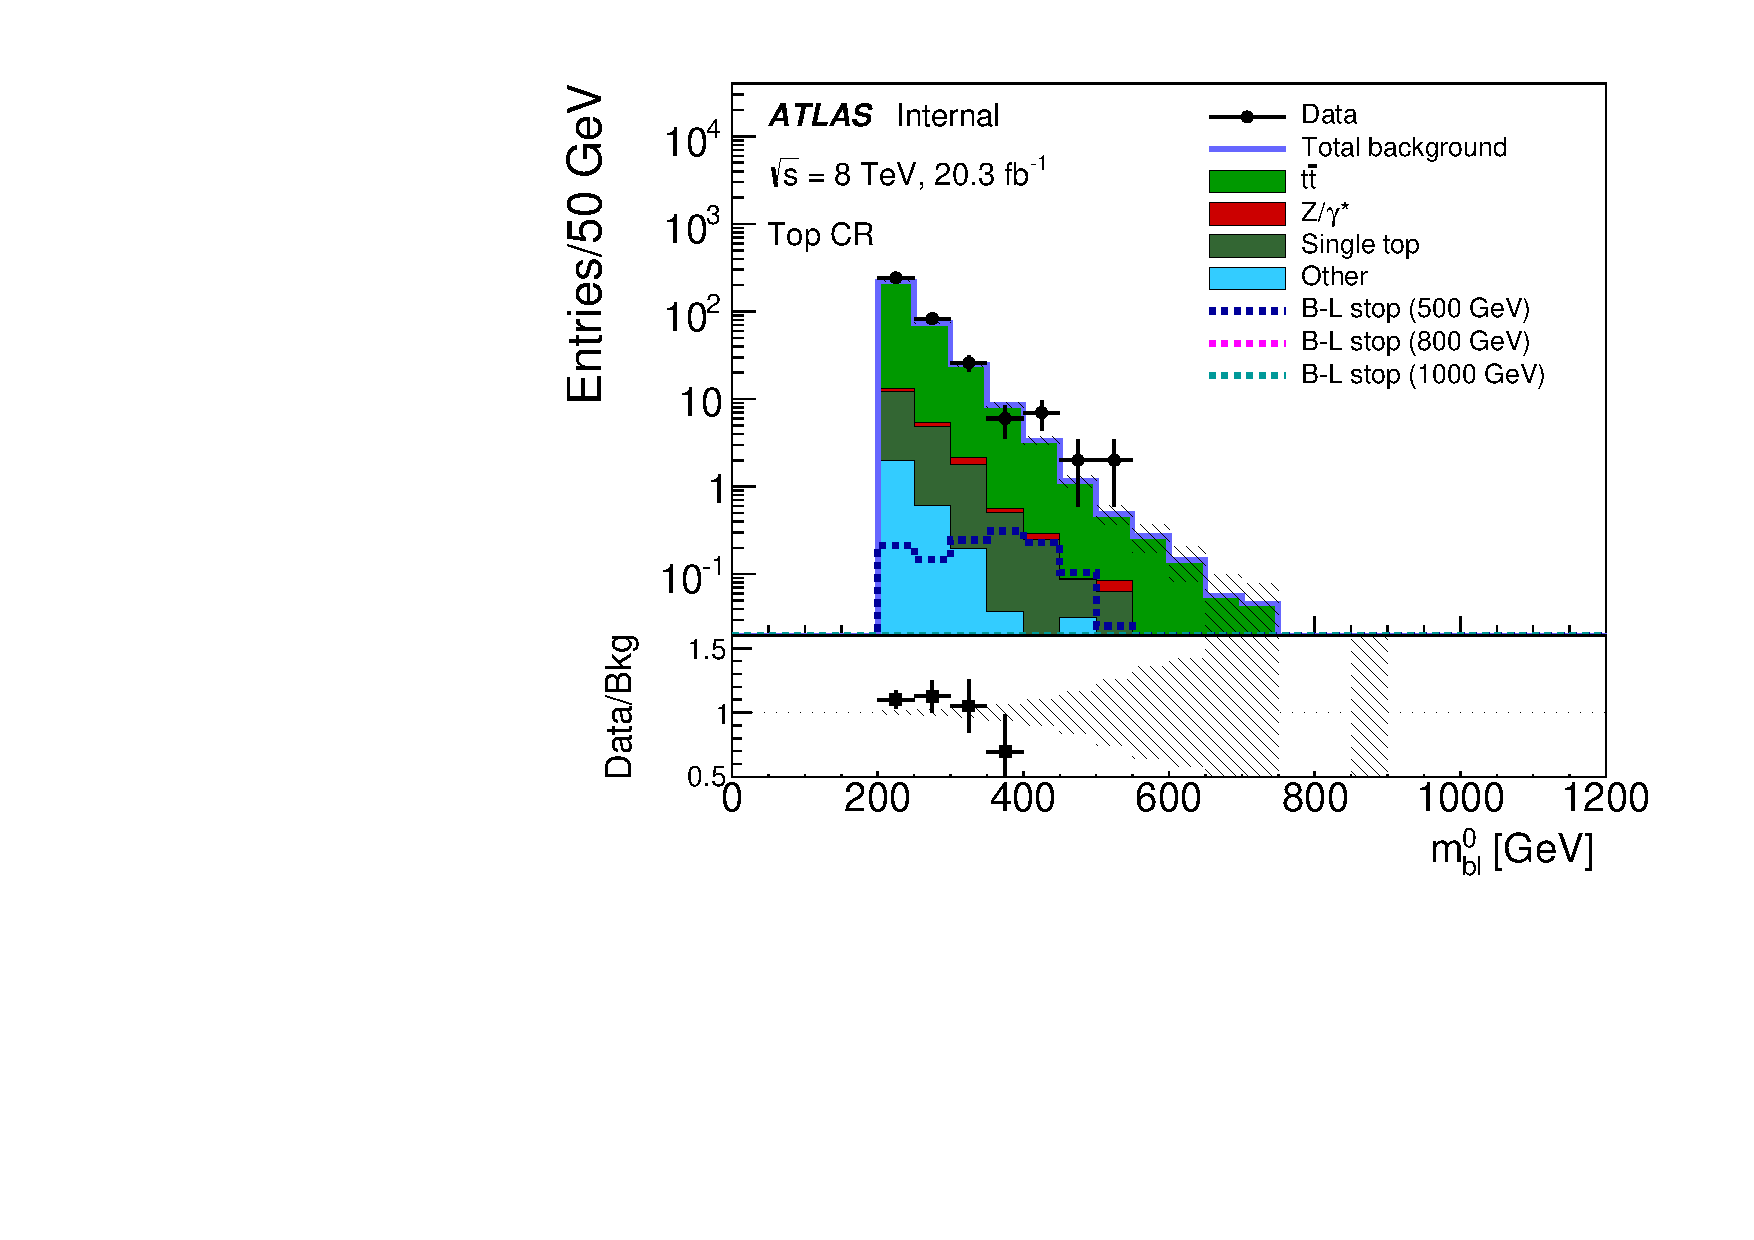
\includegraphics[width=0.48\textwidth, clip=true, trim=0 0 1cm 0]
      {figs/blstop/w_data__no_k_factor__dists/flavor_all__mbl_0__BMINUSL_CR_TOP_MBL_200__log.pdf}
  }
  \subbottom[$Z$ CR]{
    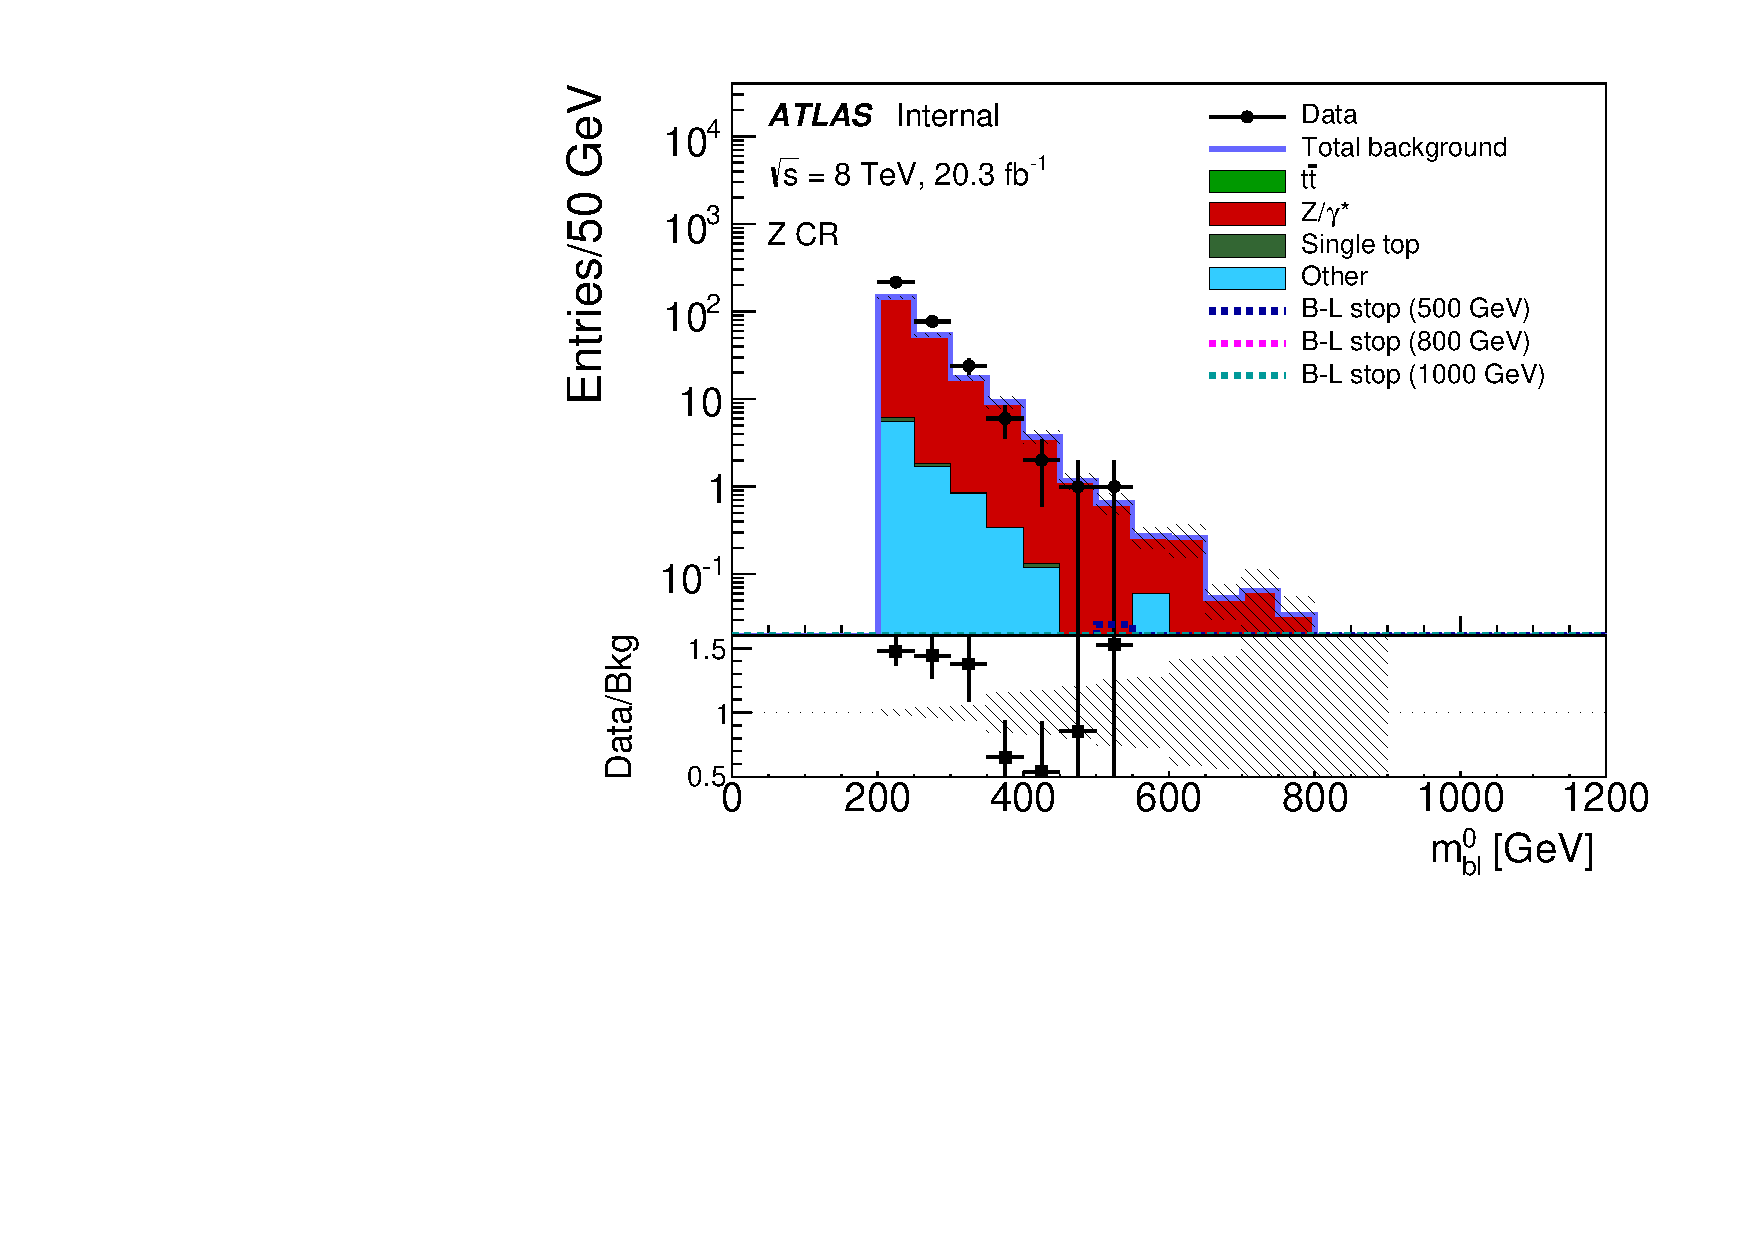
\includegraphics[width=0.48\textwidth, clip=true, trim=0 0 1cm 0]
      {figs/blstop/w_data__no_k_factor__dists/flavor_all__mbl_0__BMINUSL_CR_Z_MBL_200__log.pdf}
  }
  \caption{Expected and observed $\MBL^0$ distribution in the Top CR and
    $Z$ CR when all flavor channels are combined.
    The prediction in the Top CR shows reasonable agreement with the observed
    data.
    The background is underpredicted in the $Z$ CR.
    % In each plot, the last bin includes the overflow for values beyond the
    % maximum shown.
    The hashed error bands show only the statistical uncertainty on the
    background MC simulation samples.
    The signal models have an assumed
    $Br(\tilde{t}\rightarrow be) = Br(\tilde{t}\rightarrow b\mu) = 0.5$.
  }
  \label{fig:cr_mbl_0__no_norm_factor}
  %%
\end{figure}

After applying the $k_Z$ normalization factor the $\MBL^0$ distributions in
the Top CR and $Z$ CR are shown in Figure~\ref{fig:cr_mbl_0__w_norm_factor}.
While the prediction is roughly unchanged in the Top CR, the prediction in the
$Z$ CR shows much better agreement with the data.
The expected and observed event yields in the two CRs, broken out by background
production process, are shown in Table~\ref{tab:region_contributions_cr}.

\begin{figure}
  \centering
  \subbottom[Top CR]{
    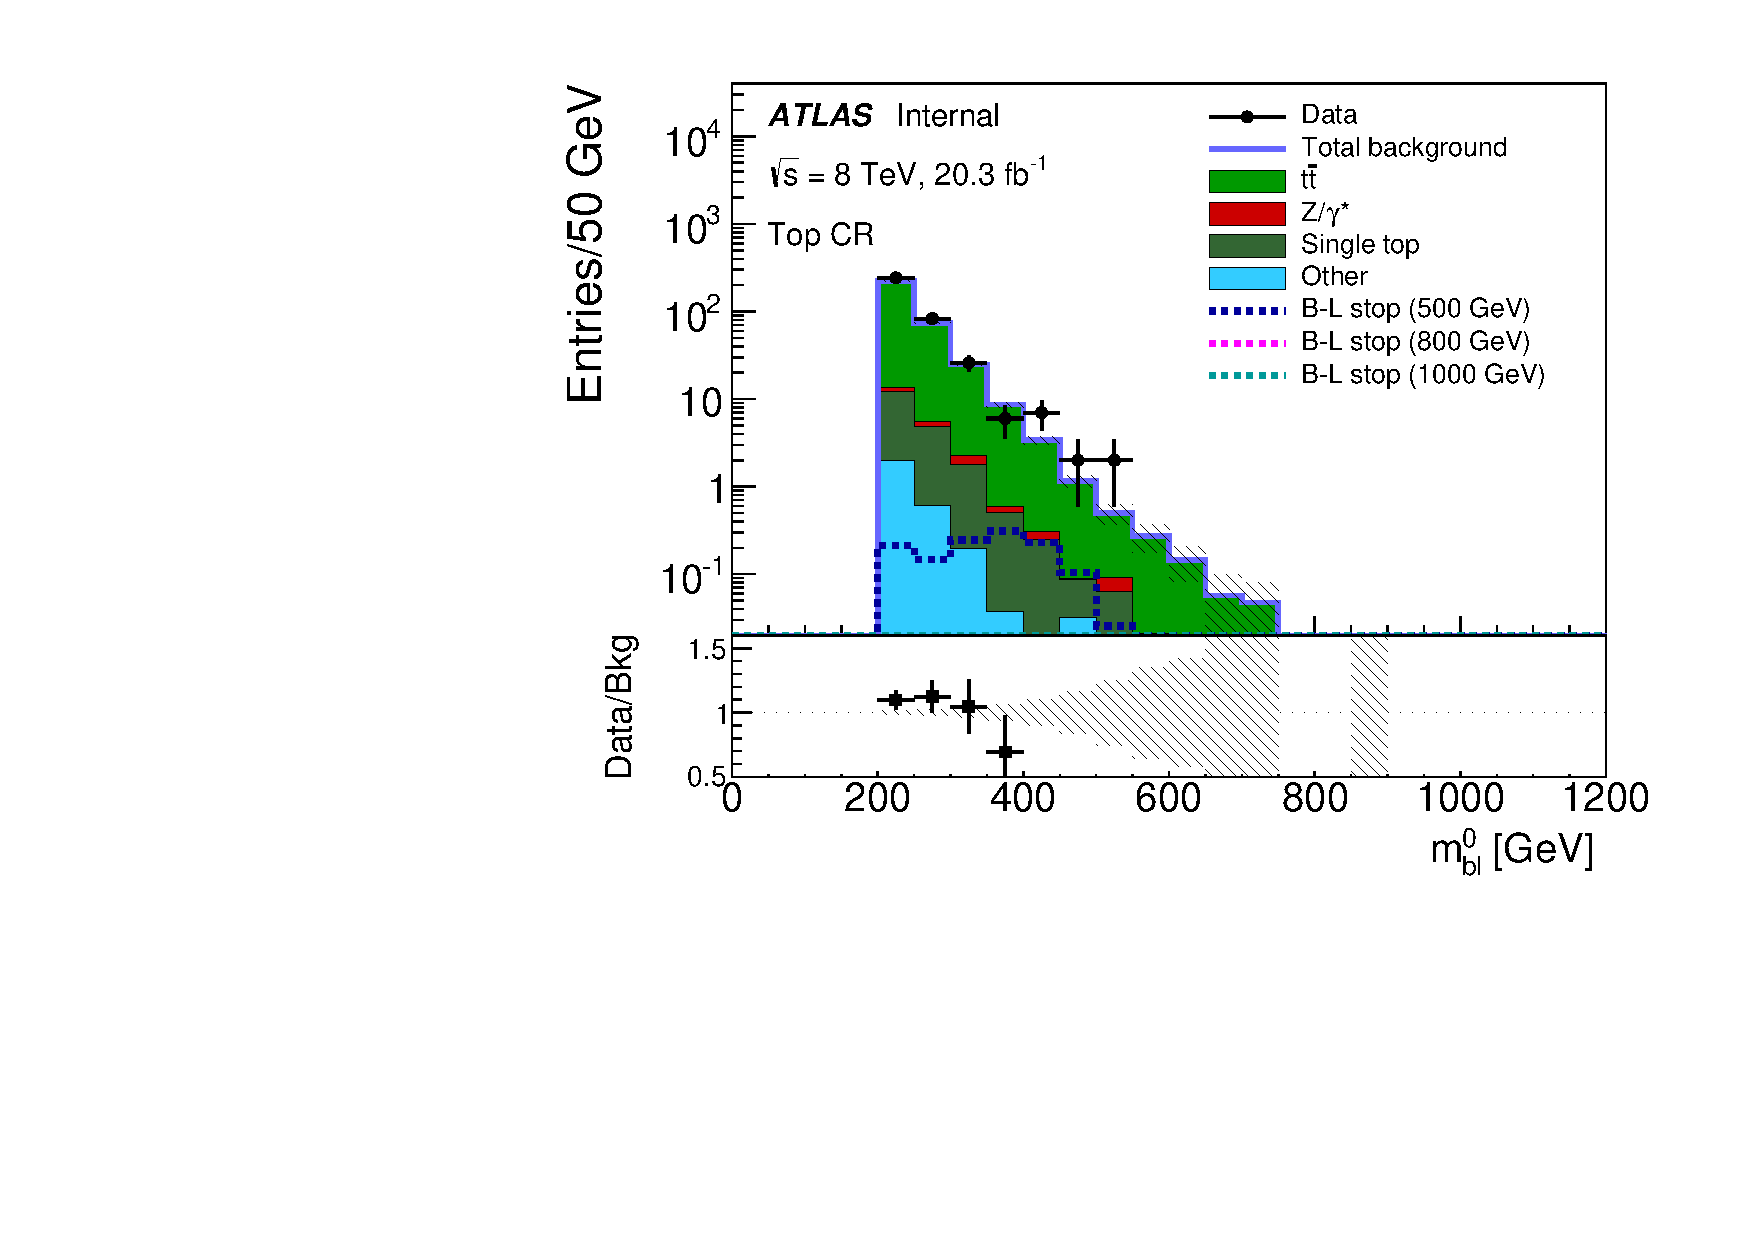
\includegraphics[width=0.48\textwidth, clip=true, trim=0 0 1cm 0]
      {figs/blstop/w_data__w_k_factor__dists/flavor_all__mbl_0__BMINUSL_CR_TOP_MBL_200__log.pdf}
  }
  \subbottom[$Z$ CR]{
    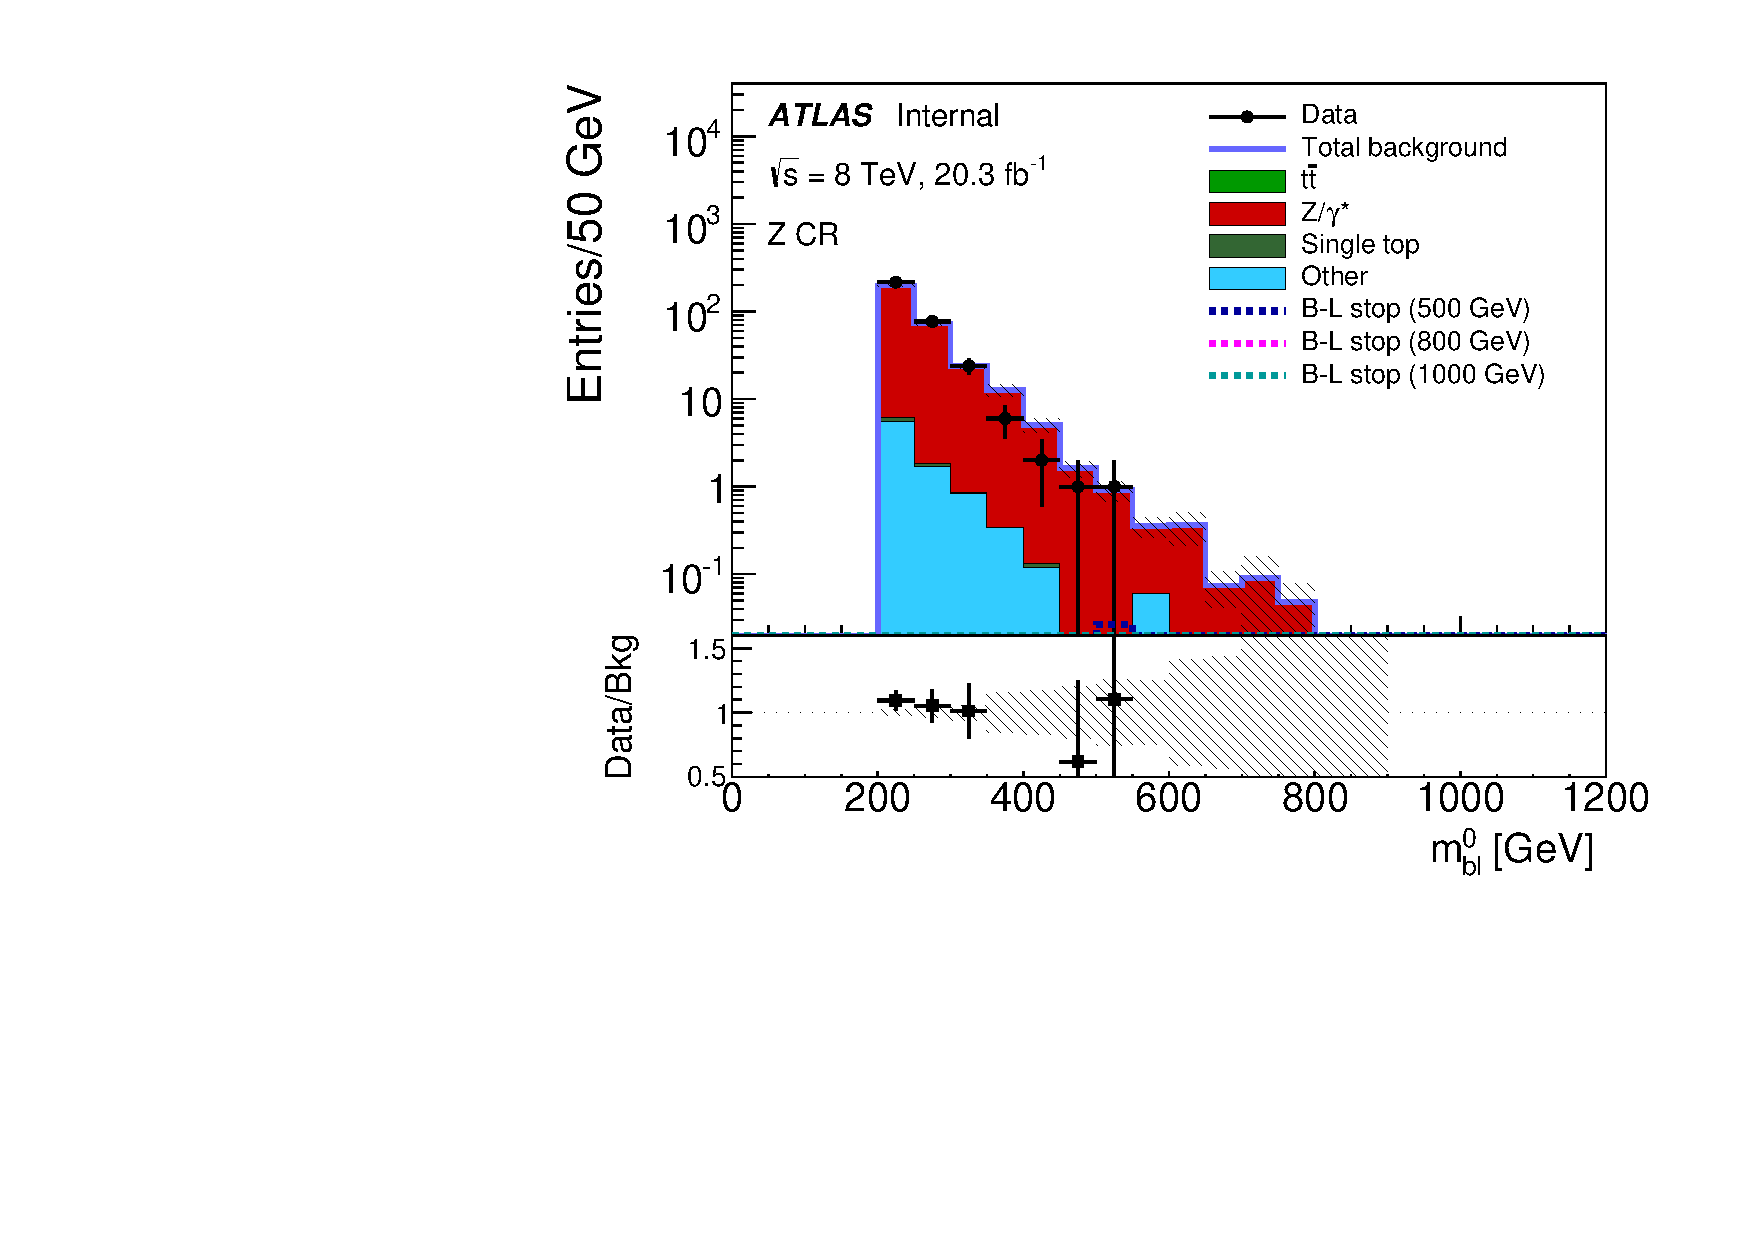
\includegraphics[width=0.48\textwidth, clip=true, trim=0 0 1cm 0]
      {figs/blstop/w_data__w_k_factor__dists/flavor_all__mbl_0__BMINUSL_CR_Z_MBL_200__log.pdf}
  }
  \caption{Expected and observed $\MBL^0$ distribution in the Top CR and
    $Z$ CR after applying the $k_Z$ normalization factor derived in the $Z$ CR
    when all flavor channels are combined.
    After applying the $k_Z$ normalization factor, both CRs show reasonable
    agreement between the predicted and observed distributions.
    % In each plot, the last bin includes the overflow for values beyond the
    % maximum shown.
    The hashed error bands show only the statistical uncertainty on the
    background MC simulation samples.
    The signal models have an assumed
    $Br(\tilde{t}\rightarrow be) = Br(\tilde{t}\rightarrow b\mu) = 0.5$.
  }
  \label{fig:cr_mbl_0__w_norm_factor}
  %%
\end{figure}

\begin{table}
  \caption{Number of expected events in each of the CRs broken down by process.
    The uncertainty on the total background prediction is the MC statistical
    uncertainty only for each background process.
    The total uncertainty is obtained by summing the uncertainty on each
    background process in quadrature.
    The $k_Z$ normalization factor is applied to the \ZGAMMAJETS\ background
    yield estimate.
    % For each signal model, the ratio of expected signal events to the sum of the
    % background in each region is show in parentheses.
    {\color{red} TODO add observed number events in each CR.}
    {\color{red} TODO update with only stat uncertainty.}
    {\color{red} TODO update with breakdown by flavor channel.}
  }
  \label{tab:region_contributions_cr}
  \centering{
    \begin{tabular}{c|cc}
      \toprule
                                           & Top CR                            & $Z$ CR                            \\
      \midrule
      \TTBAR                               & $311.8$                           & $8.2$                             \\
      \ZGAMMAJETS                          & $3.1$                             & $297.9$                           \\
      Single top                           & $16.7$                            & $0.8$                             \\
      Other                                & $2.9$                             & $8.6$                             \\
      \midrule
      Total                                & \multirow{2}{*}{$334.5 \pm 93.7$} & \multirow{2}{*}{$315.6 \pm 89.5$} \\
      background                           &                                   &                                   \\
      \midrule
      \multirow{2}{*}{B-L stop (500 GeV)}  & $1.3$                             & $0.03$                            \\
                                           & ($< 0.01$)                        & ($< 0.01$) \vspace{1ex}           \\
      \multirow{2}{*}{B-L stop (800 GeV)}  & $< 0.01$                          & $< 0.01$                          \\
                                           & ($< 0.01$)                        & ($< 0.01$) \vspace{1ex}           \\
      \multirow{2}{*}{B-L stop (1000 GeV)} & $< 0.01$                          & $< 0.01$                          \\
                                           & ($< 0.01$)                        & ($< 0.01$) \vspace{1ex}           \\
      \bottomrule
    \end{tabular}
  }
\end{table}

{\color{red} TODO add plots showing pre-fit agreement in CRs}

%% -----------------------------------------------------------------------------
\FloatBarrier
\subsection{Validation regions}
\label{sec:vr}

The normalization factors for the \TTBAR\ and \ZGAMMAJETS\ background processes
are determined using the observed data in the CRs, then used to estimate the
background contribution in the SRs.
To show these normalization factors are valid in regions of kinematic space away
from the CRs, Validation regions (VRs), which are orthogonal to the CRs and SRs
are defined, where the background prediction can be compared with the
observation.
These VRs have low expected signal contamination, but do not need to be pure in
any particular background process, as is required of the CRs.
Since this analysis targets stops with reasonably high mass, all VRs require
$\MBL^0 \geq 200 \GeV$ as is required in the CRs.

Three orthogonal VRs are defined to validate the \TTBAR\ background estimate,
labeled Top VR 1, Top VR 2, and Top VR 3.
Top VR 1 is constructed by reversing the cut on \METSIG\ in the Top CR.
That is, Top VR 1 requires events have $\METSIG < 4 \GeV^{1/2}$, and is
otherwise identical to the Top CR.
Top VR 2 is obtained by reversing the \MBLASYM\ requirement in the Top CR and
relaxing the \METSIG\ requirement.
Top VR 3 is intended to validate the extrapolation of the \TTBAR\ background
prediction from the low \HT\ Top CR to the high \HT\ region of the SRs.
The Top VR 3 region is obtained by reversing the \HT\ selection criteria from
the Top VR 2 region, giving a region with $\MBLASYM > 0.2$ and $\HT > 500 \GeV$.

The $Z$ VR is used to validate the extrapolation of the \ZGAMMAJETS\ background
prediction from the $Z$ CR to kinematic regions higher \HT.
This region is constructed by reversing the \HT\ selection criteria from the
$Z$ CR, and relaxing the \METSIG\ requirement.
The full VR selection criteria are outlined along with the other analysis
regions in Table~\ref{tab:regions} and Figure~\ref{fig:region_coverage}.
The expected and observed event yields in the VRs, broken out by background
production process, are shown in Table~\ref{tab:region_contributions_vr}.
The agreement between the observed and predicted yields and distributions in the
VRs are explored in more detail in Section~\ref{sec:bkg_fit}.

\begin{table}
  \caption{Number of expected events in each of the VRs broken down by process.
    The uncertainty on the total background prediction is the MC statistical
    uncertainty only for each background process.
    The total uncertainty is obtained by summing the uncertainty on each
    background process in quadrature.
    The $k_Z$ normalization factor is applied to the \ZGAMMAJETS\ background
    yield estimate.
    For each signal model, the ratio of expected signal events to the sum of the
    background in each region is show in parentheses.
    {\color{red} TODO add observed number events in each VR.}
    {\color{red} TODO update with only stat uncertainty.}
    {\color{red} TODO update with breakdown by flavor channel.}
  }
  \label{tab:region_contributions_vr}
  \centering{
    \begin{tabular}{c|cccc}
      \toprule
                                             & Top VR 1                           & Top VR 2                           & Top VR 3                         & $Z$ VR                \\
      \midrule
      \TTBAR                                 & $542.6$                            & $447.3$                            & $48.9$                           & $2.7$                 \\
      \ZGAMMAJETS                            & $58.4$                             & $59.6$                             & $1.5$                            & $115.5$               \\
      Single top                             & $23.0$                             & $56.5$                             & $14.1$                           & $0.3$                 \\
      Other                                  & $4.8$                              & $8.2$                              & $2.0$                            & $6.4$                 \\
      \midrule
      Total                                  & \multirow{2}{*}{$628.8 \pm 163.9$} & \multirow{2}{*}{$571.6 \pm 136.5$} & \multirow{2}{*}{$66.6 \pm 15.3$} & \multirow{2}{*}{$125.0 \pm 34.7$}               \\
      background                             &                                    &                                    &                                  & \\
      \midrule
      \multirow{2}{*}{B-L stop (500 GeV)}    & $5.1$                              & $2.4$                              & $10.7$                           & $3.8$                 \\
                                             & ($< 0.01$)                         & ($<0.01$)                          & ($0.2$)                          & ($0.03$) \vspace{1ex} \\
      \multirow{2}{*}{B-L stop (800 GeV)}    & $< 0.01$                           & $< 0.01$                           & $0.6$                            & $0.02$   \\
                                             & ($< 0.01$)                         & ($< 0.01$)                         & ($< 0.01$)                       & ($< 0.01$) \vspace{1ex} \\
      \multirow{2}{*}{B-L stop (1000 GeV)}   & $< 0.01$                           & $< 0.01$                           & $0.1$                            & $< 0.01$                     \\
                                             & ($< 0.01$)                         & ($< 0.01$)                         & ($< 0.01$)                       & ($< 0.01$)
      \vspace{1ex} \\
      \bottomrule
    \end{tabular}

  }
\end{table}

%% -----------------------------------------------------------------------------
\FloatBarrier
\subsection{Background fit}
\label{sec:bkg_fit}

The normalization of the \TTBAR\ and the \ZGAMMAJETS\ backgrounds are
determined using a simultaneous fit, which takes into account
cross-contamination of the different background processes between the
CRs as well as the statistical and systematic uncertainties (described in
Section~\ref{sec:systematics}).
The fit is implemented using the HistFitter version~1.2.1, a framework for
statistical data analysis~\cite{Baak:2014wma}.
The remaining background estimates, due to  single top and other SM processes,
are taken from the MC simulation.

The background-only estimate is performed using a maximum likelihood fit
to the data in the Top and Z CRs.
The three flavor channels ($ee$, $\mu\mu$, and $e\mu$) are summed over, and the
total event yield in these regions are considered.
The predicted event yield for a background process $p$ (\TTBAR\ or \ZGAMMAJETS)
in a particular region $r$ is $\mu_{p} \cdot N_{r,p}^\mathrm{MC}$, where
$N_{r,p}^\mathrm{MC}$ is the number of events from process $p$ in region $r$
predicted by the MC simulation estimate, after applying all the relevant
scale factors and efficiencies.
$\mu_{p}$ is a strength parameter for each process which enters the likelihood
fit, which is used to model any under/over-prediction in the MC simulation
which is assumed to be constant across all regions.
A strength parameter is defined for the \TTBAR\ and \ZGAMMAJETS\ background
predictions, $\mu_{\TTBAR}$ and $\mu_\mathrm{Z}$ respectively.

The background fit is performed by first summing the total background estimate
for all backgrounds in each of the CRs.
The strength parameters are varied until to obtain the best agreement between
the observed event yields and the background predictions.
The systematic uncertainties are treated as Gaussian nuisance parameters.
The background only fit finds that the best fit values for $\mu_{\TTBAR}$ and
$\mu_\mathrm{Z}$ are $1.11 \pm 0.14$ and $1.43 \pm 0.19$ respectively.

The number of observed events as well as the post-fit expected number
of events in each of the CRs and VRs are shown in
Table~\ref{tab:bkg_only_fit_results}.
The agreement between the observed number of events and the fitted event
yields in the VRs is summarized in Figure~\ref{fig:pull_dist_vr}.
Using the fitted backgrounds, the dominant process in the same-flavor
channels of the SRs is \ZGAMMAJETS\ followed by single top and
\TTBAR. In the $e\mu$ channel, the \ZGAMMAJETS\ background does
not contribute, thus, the largest backgrounds are single top and \TTBAR.

As a result of the fit, the \ZGAMMAJETS\ background is scaled up by
approximately 40\%. Due to this large normalization factor, the background is
over-predicted in the $Z$ VR. This over-prediction is taken as an additional
systematic uncertainty, described in Section~\ref{sec:systematics}.

% - - - - - - - - - - - - - - - - - - - - - - - - - - - - - - - - - - - - - - -
\begin{table}[ht]
  \caption{The observed and expected event yields in the CRs and VRs. The
    expected event yields are shown before and after a fit to the data in
    the CRs. The fitted background yields in the CRs match the observed
    number of events in data by construction.
  }
  \label{tab:bkg_only_fit_results}
  %
  \begin{center}
    \begin{tabular}{lrrrrrr}
      \toprule
                         & Top CR           & Z CR            & Top VR 1       & Top VR 2      & Top VR 3        & Z VR            \\
      \midrule
      Observed           & $369$            & $327$           & $645$          & $606$         & $67$            & $101$           \\
      \midrule
      Fitted background  & $369   \pm 19$   & $327  \pm 18$   & $690  \pm 50$  & $630 \pm 40$  & $72   \pm 5$    & $130  \pm 60$   \\
      \midrule
      Fitted \TTBAR      & $346   \pm 19$   & $9.1  \pm 0.7$  & $600  \pm 40$  & $497 \pm 35$  & $54   \pm 5$    & $2.99 \pm 0.24$ \\
      Fitted \ZGAMMAJETS & $3.2   \pm 0.5$  & $309  \pm 18$   & $63   \pm 5$   & $64  \pm 5$   & $1.5  \pm 0.8$  & $120  \pm 60$   \\
      Single top         & $16.7  \pm 2.0$  & $0.83 \pm 0.09$ & $23.0 \pm 2.6$ & $56  \pm 6$   & $14.1 \pm 1.9$  & $0.32 \pm 0.04$ \\
      Other              & $2.83  \pm 0.27$ & $8.64 \pm 1.0$  & $4.7  \pm 0.4$ & $8.2 \pm 0.8$ & $2.03 \pm 0.27$ & $6.4  \pm 0.7$  \\
      \midrule
      Input SM           & $330$            & $230$           & $614$          & $557$         & $66$            & $93$            \\
      \midrule
      Input \TTBAR       & $310$            & $8.2$           & $543$          & $447$         & $49$            & $2.7$           \\
      Input \ZGAMMAJETS  & $2.2$            & $220$           & $44$           & $45$          & $1.1$           & $83$            \\
      Input single top   & $17$             & $0.8$           & $23$           & $57$          & $14$            & $0.30$          \\
      Input other        & $2.8$            & $8.6$           & $4.7$          & $8.2$         & $2.0$           & $6.40$          \\
      \bottomrule
    \end{tabular}
  \end{center}
\end{table}

\begin{figure}[ht]
\centering
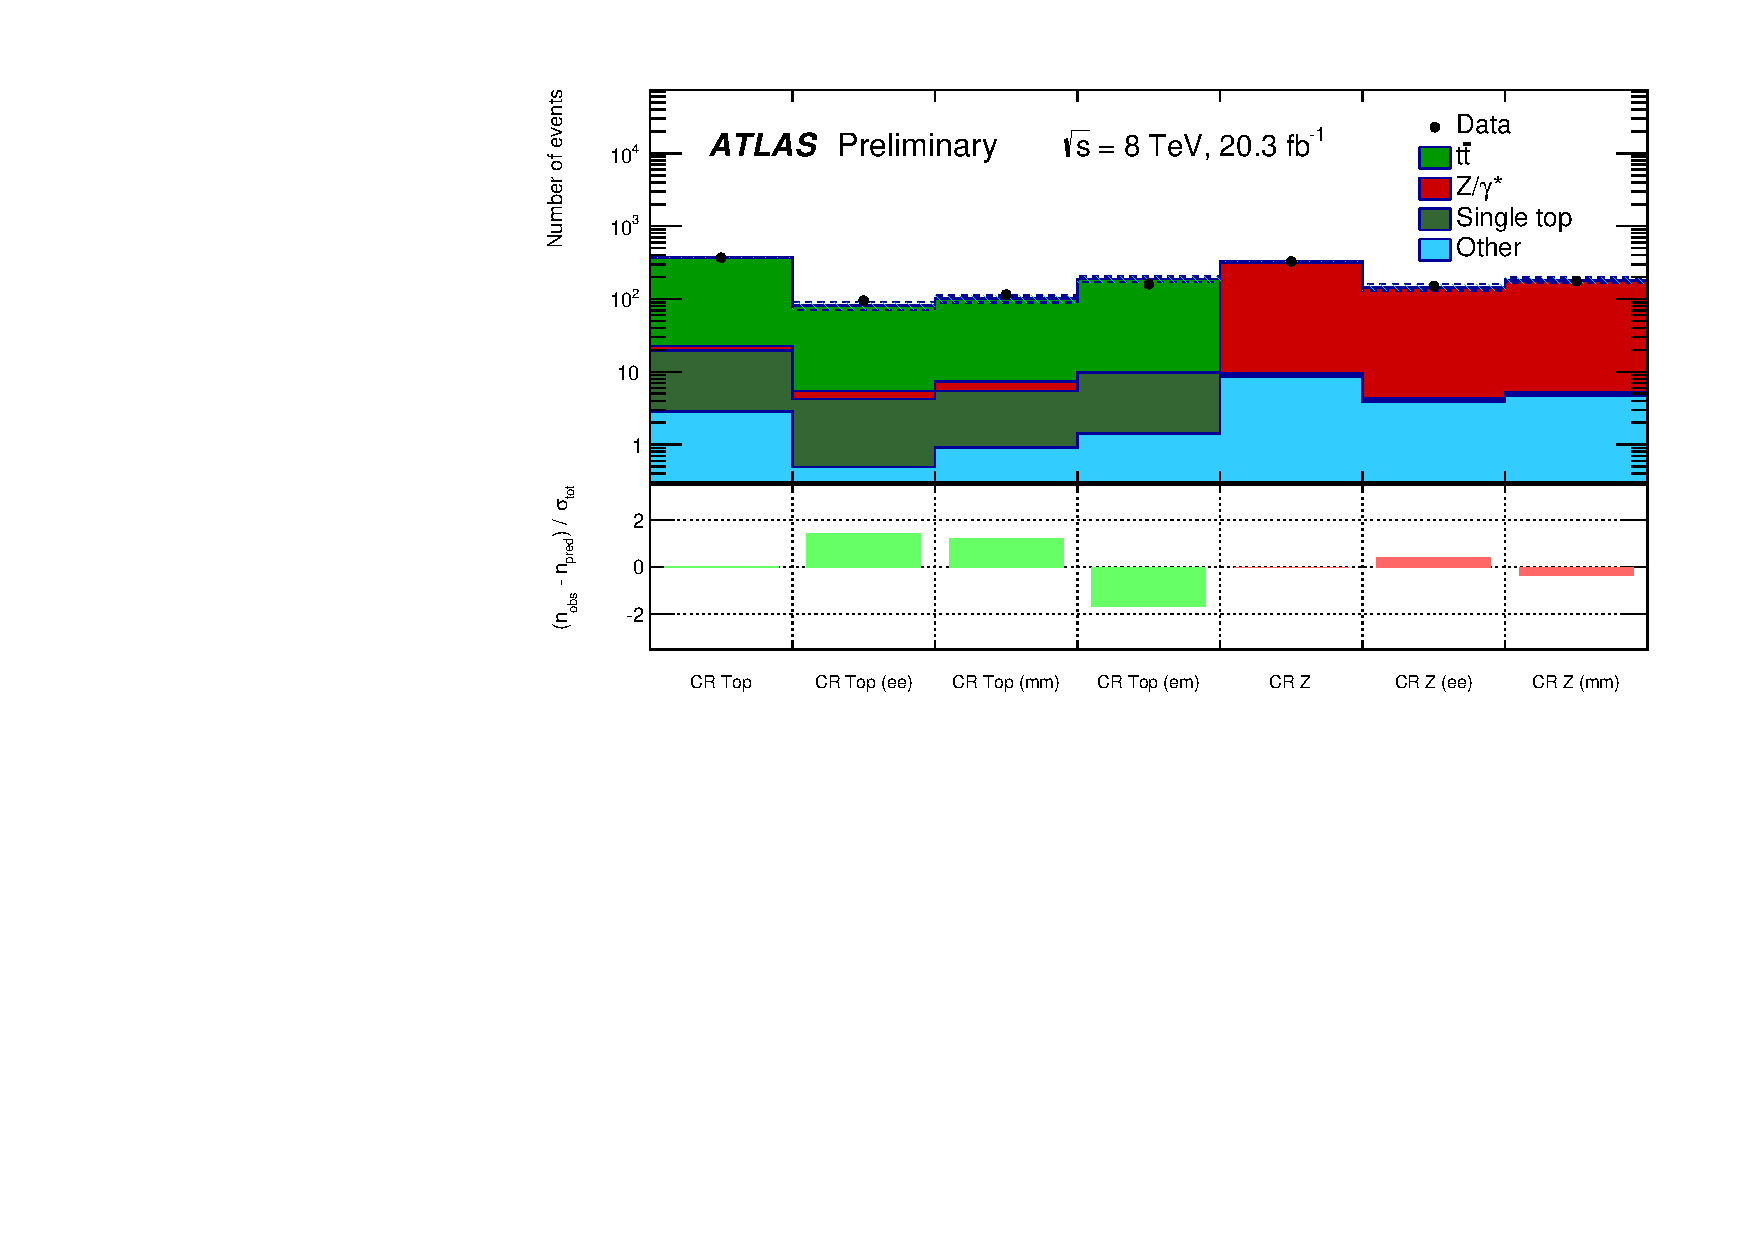
\includegraphics[width=\textwidth]{figs/blstop/histpull_CR_detailed.pdf}
\caption{The top of this plot shows the number of observed and expected
  events in the CRs, and broken down by flavor channel.
  The uncertainty band includes the statistical uncertainty as well as the
  systematic uncertainty (described in Section~\ref{sec:systematics}). The
  bottom of the plot shows the deviation of that channel's prediction
  from the observed number of events divided by the uncertainty on the
  prediction. The normalization of the background yields are determined
  by fitting the \TTBAR\ and \ZGAMMAJETS\ backgrounds to the observed
  data in the two CRs, so the Top CR and $Z$ CR bins have perfect agreement by
  construction.
}
\label{fig:pull_dist_cr}
\end{figure}

\begin{figure}[ht]
\centering
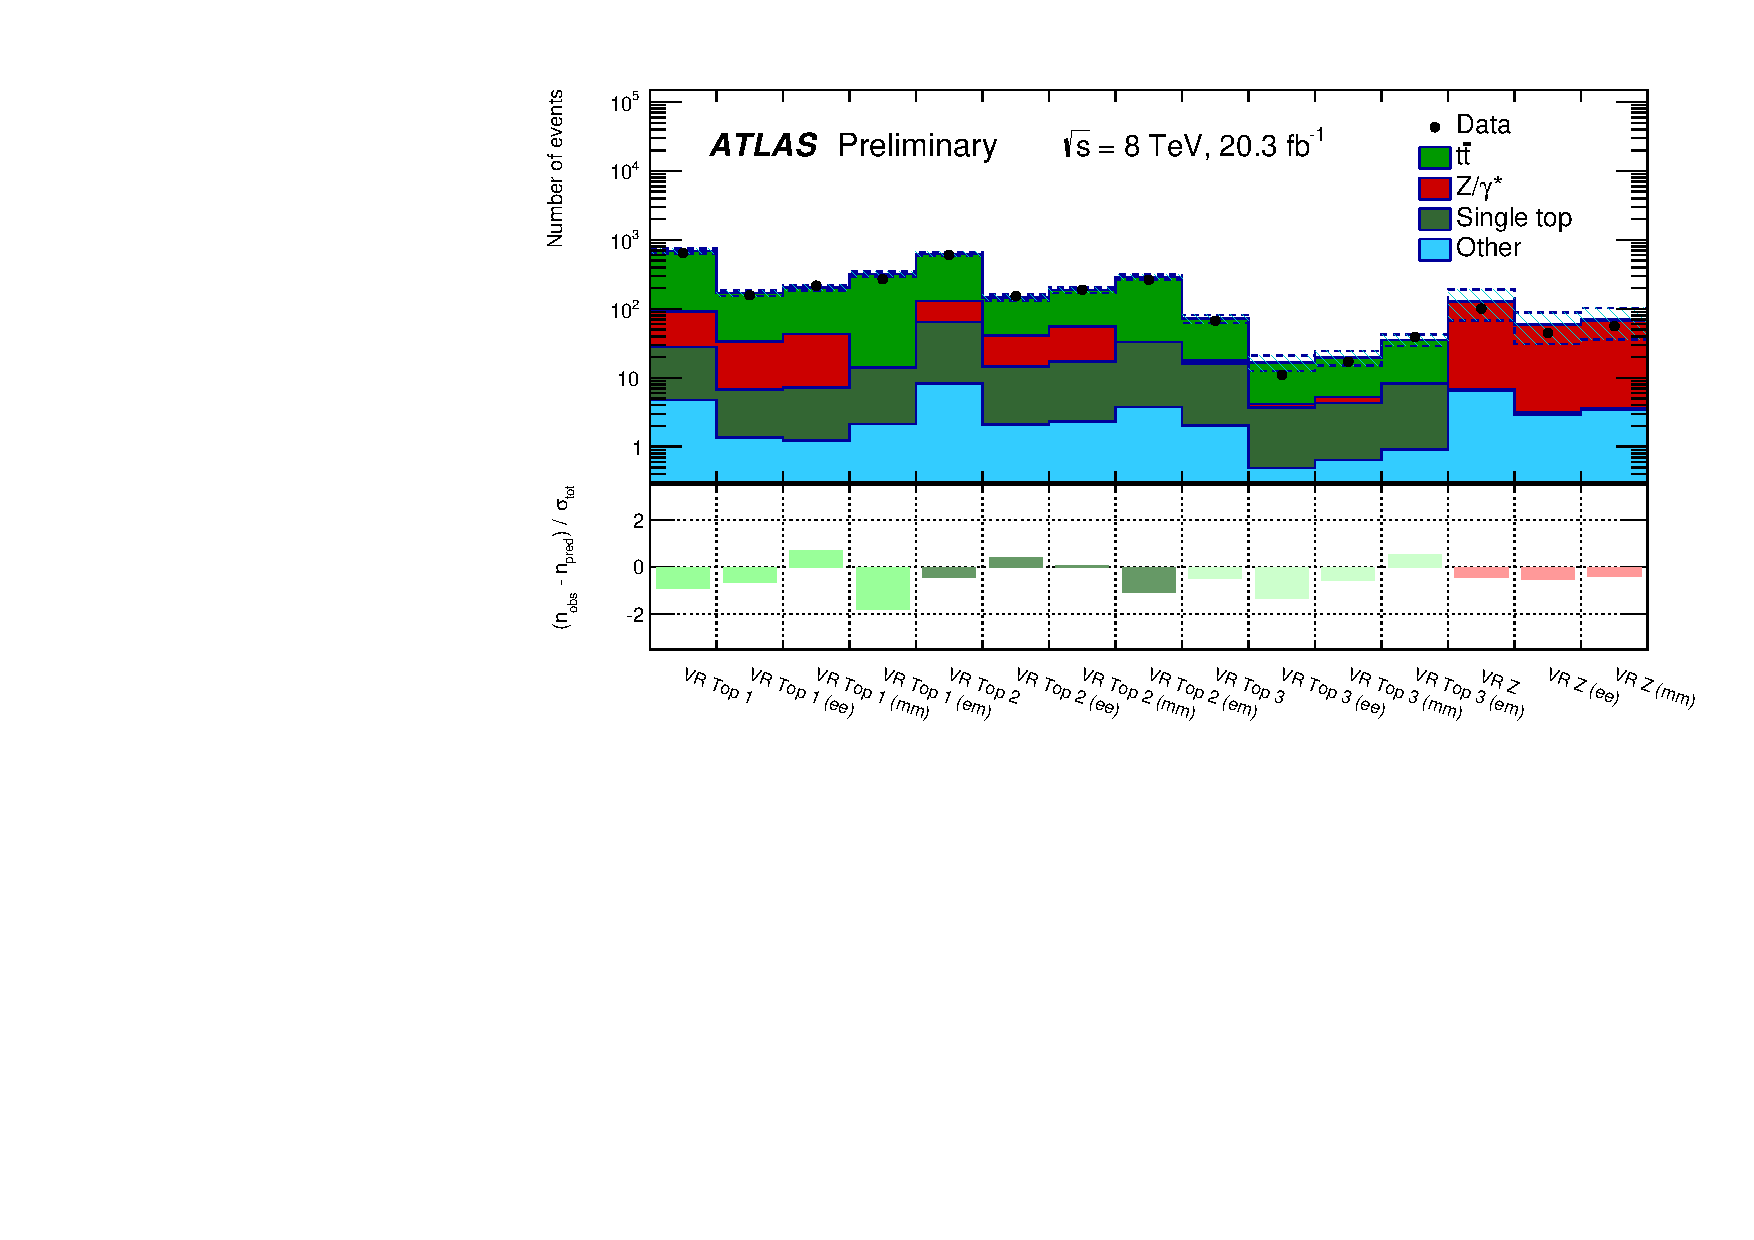
\includegraphics[width=\textwidth]{figs/blstop/histpull_VR_detailed.pdf}
\caption{The top of this plot shows the number of observed and expected
  events in the VR, and broken down by flavor channel.
  The uncertainty band includes the statistical uncertainty as well as the
  systematic uncertainty (described in Section~\ref{sec:systematics}). The
  bottom of the plot shows the deviation of that channel's prediction
  from the observed number of events divided by the uncertainty on the
  prediction. The normalization of the background yields are determined
  by fitting the \TTBAR\ and \ZGAMMAJETS\ backgrounds to the observed
  data in the two CRs.
}
\label{fig:pull_dist_vr}
\end{figure}

The extrapolation from low \HT\ CRs to the high \HT\ region
where the SRs are located is validated using the Top VR 3
and $Z$ VR. These validation regions show fair
agreement between the observed and predicted event yields as well as
for the shape of the $\MBL^{0}$ and \HT\ distributions as shown in
Figures~\ref{fig:mbl_vr} and~\ref{fig:ht_vr}.

\begin{figure}
  \centering
  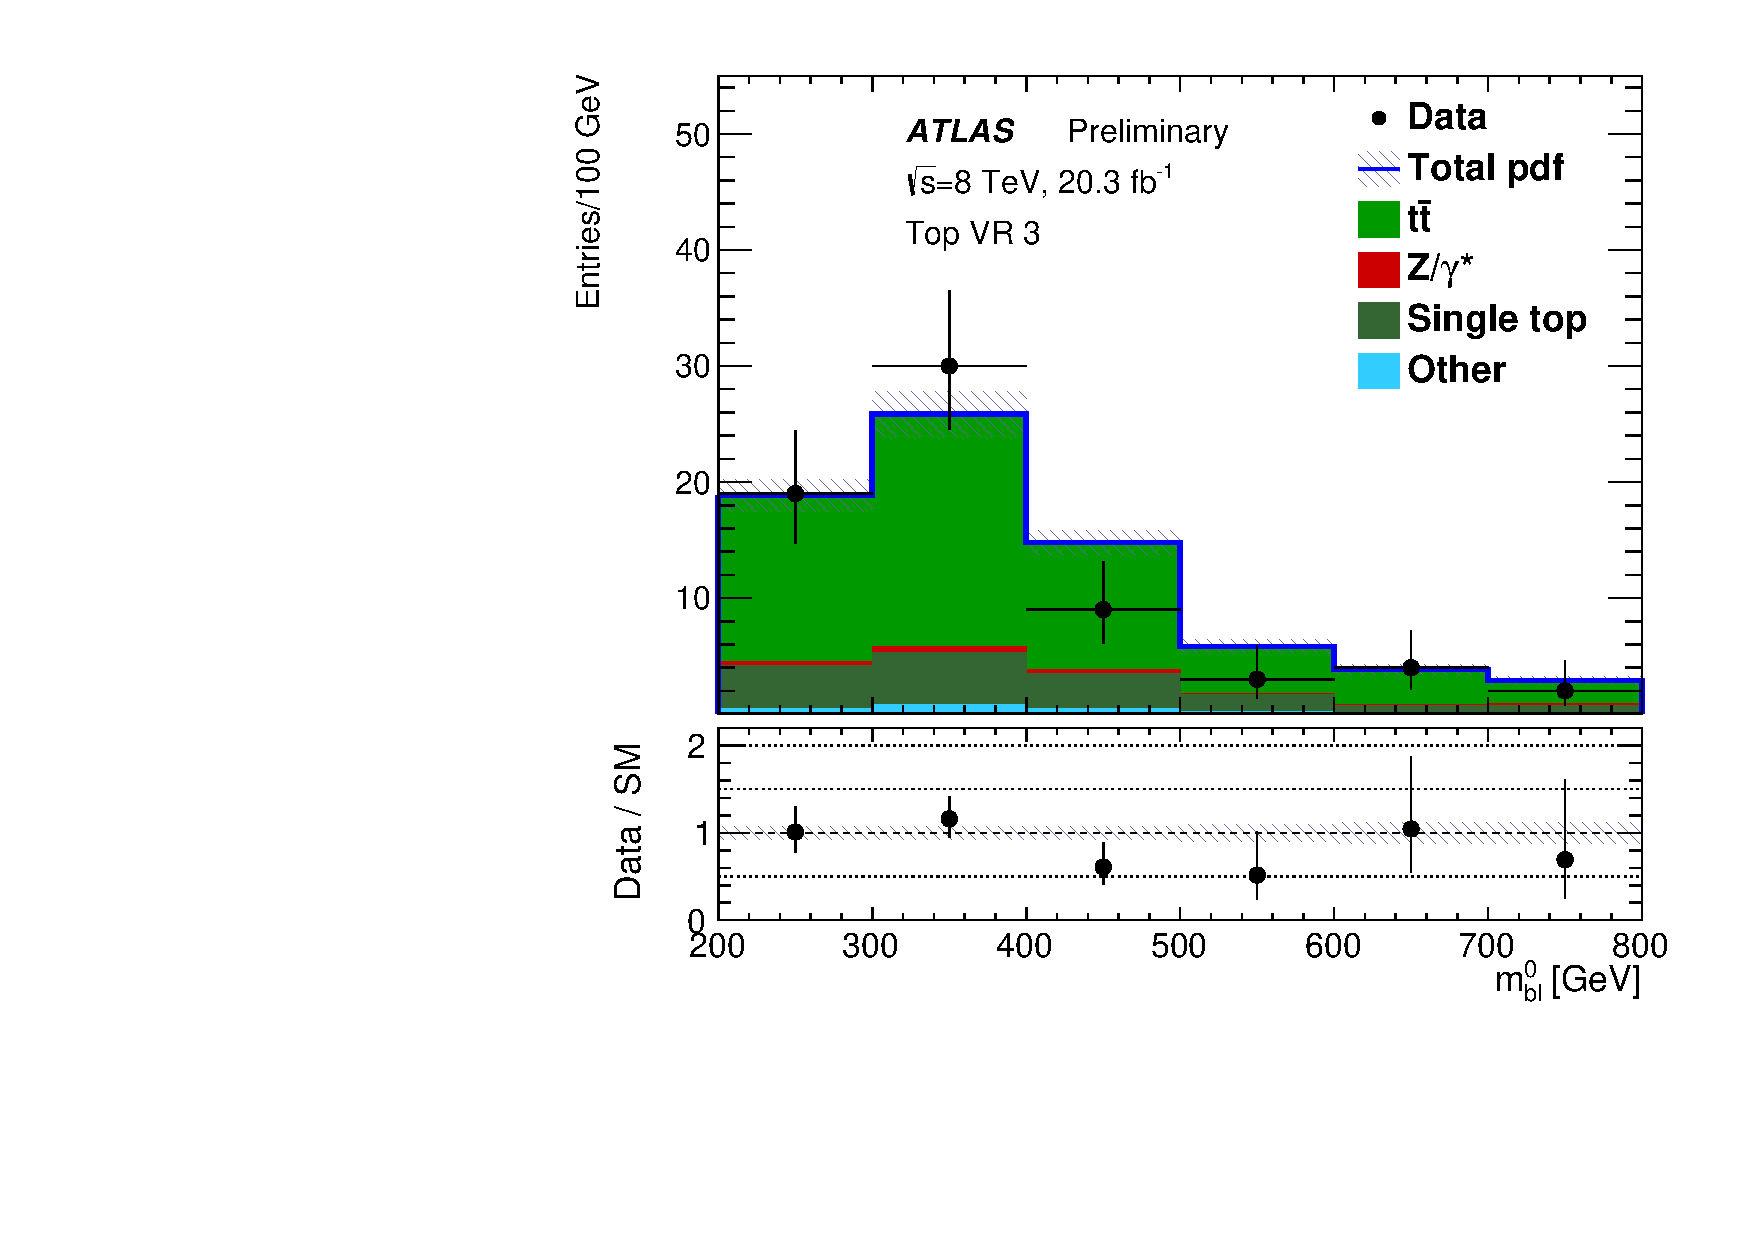
\includegraphics[width=0.48\textwidth]{figs/blstop/vr_top_3_mbl_0.pdf}
  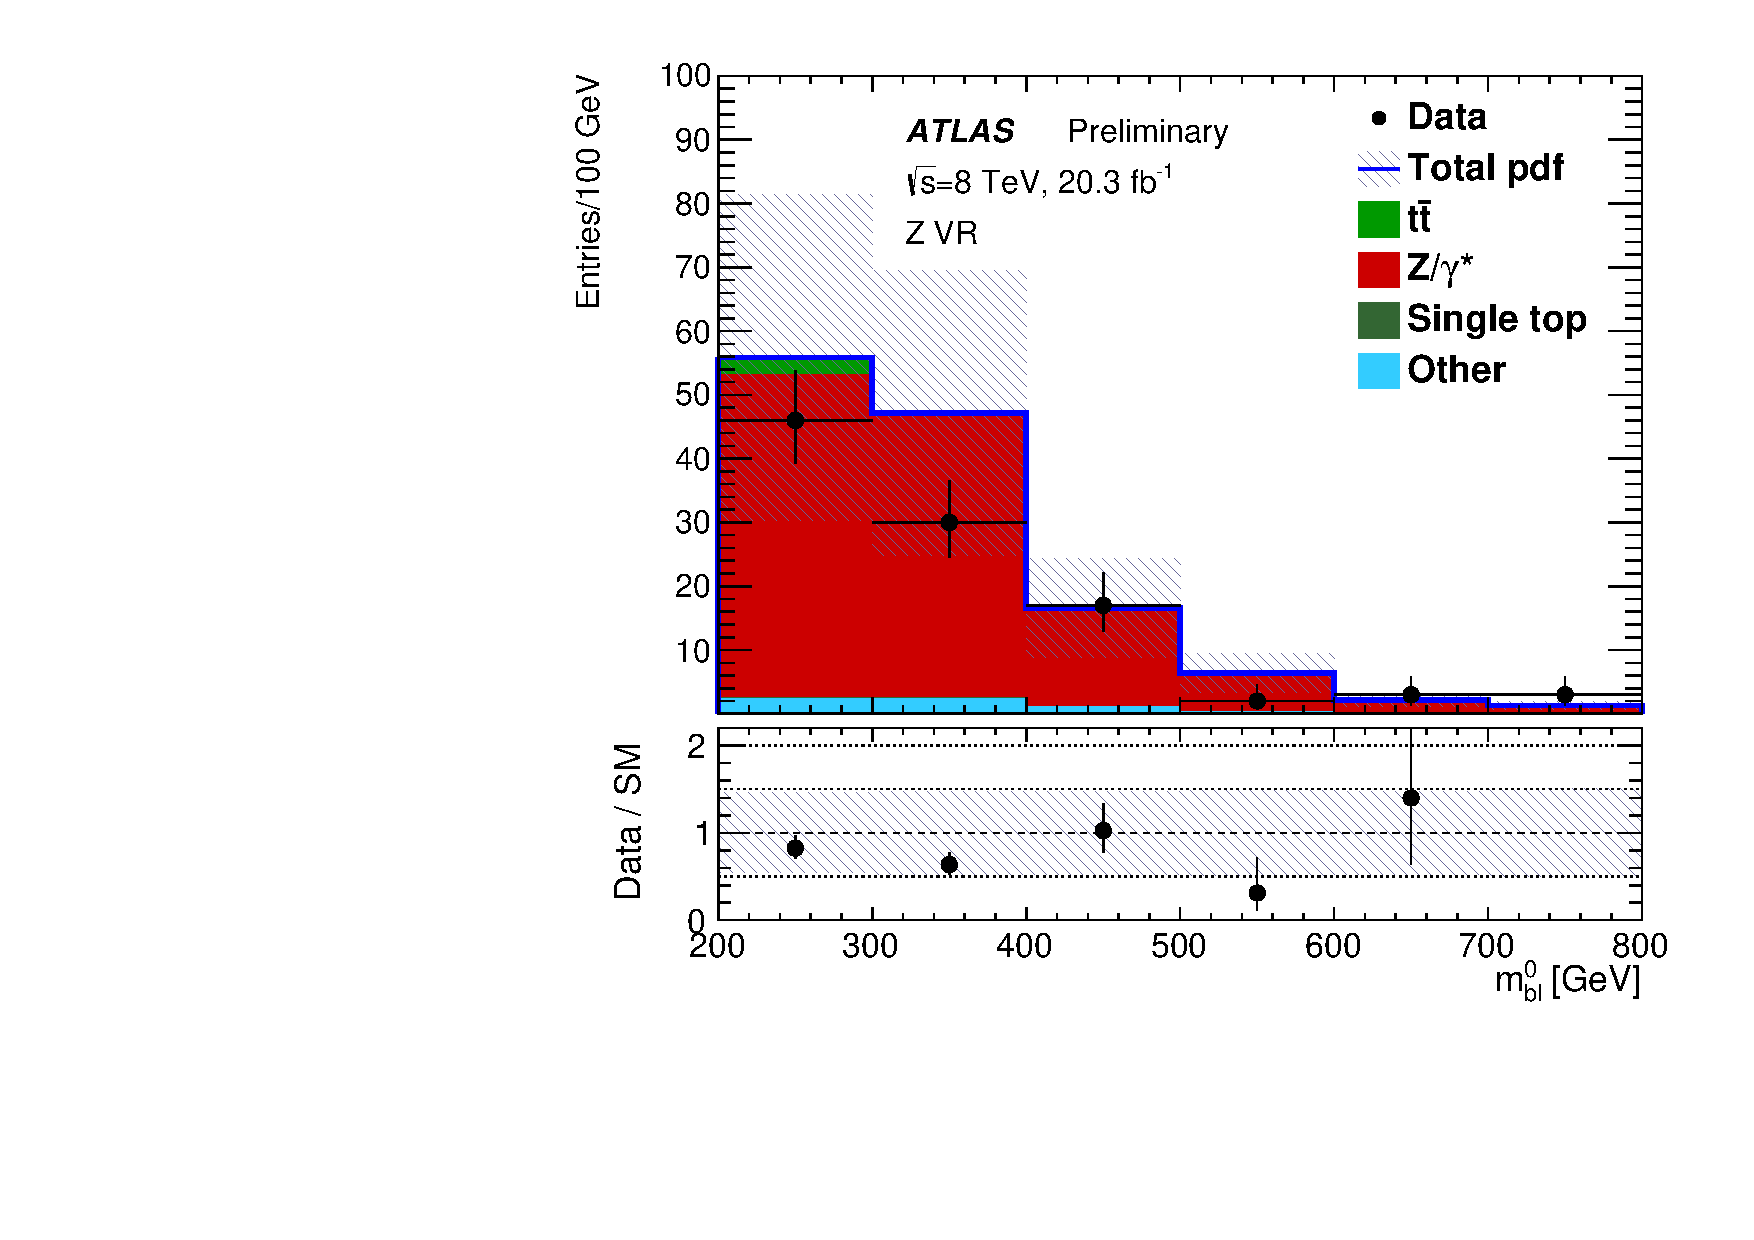
\includegraphics[width=0.48\textwidth]{figs/blstop/vr_Z_mbl_0.pdf}
  \caption{The $\MBL^0$ distribution in Top VR 3 (left) and $Z$ VR (right).
    The Standard Model background prediction is shown after setting the
    normalization of the \TTBAR\ and \ZGAMMAJETS\ backgrounds based on the
    observed data in the CRs. The hashed bands show the uncertainty on the
    fitted background prediction including all statistical and systematics
    uncertainties.
    The bottom of each plot shows the ratio of the observed data to the
    Standard Model background prediction.
  }
  \label{fig:mbl_vr}
\end{figure}

\begin{figure}
  \centering
  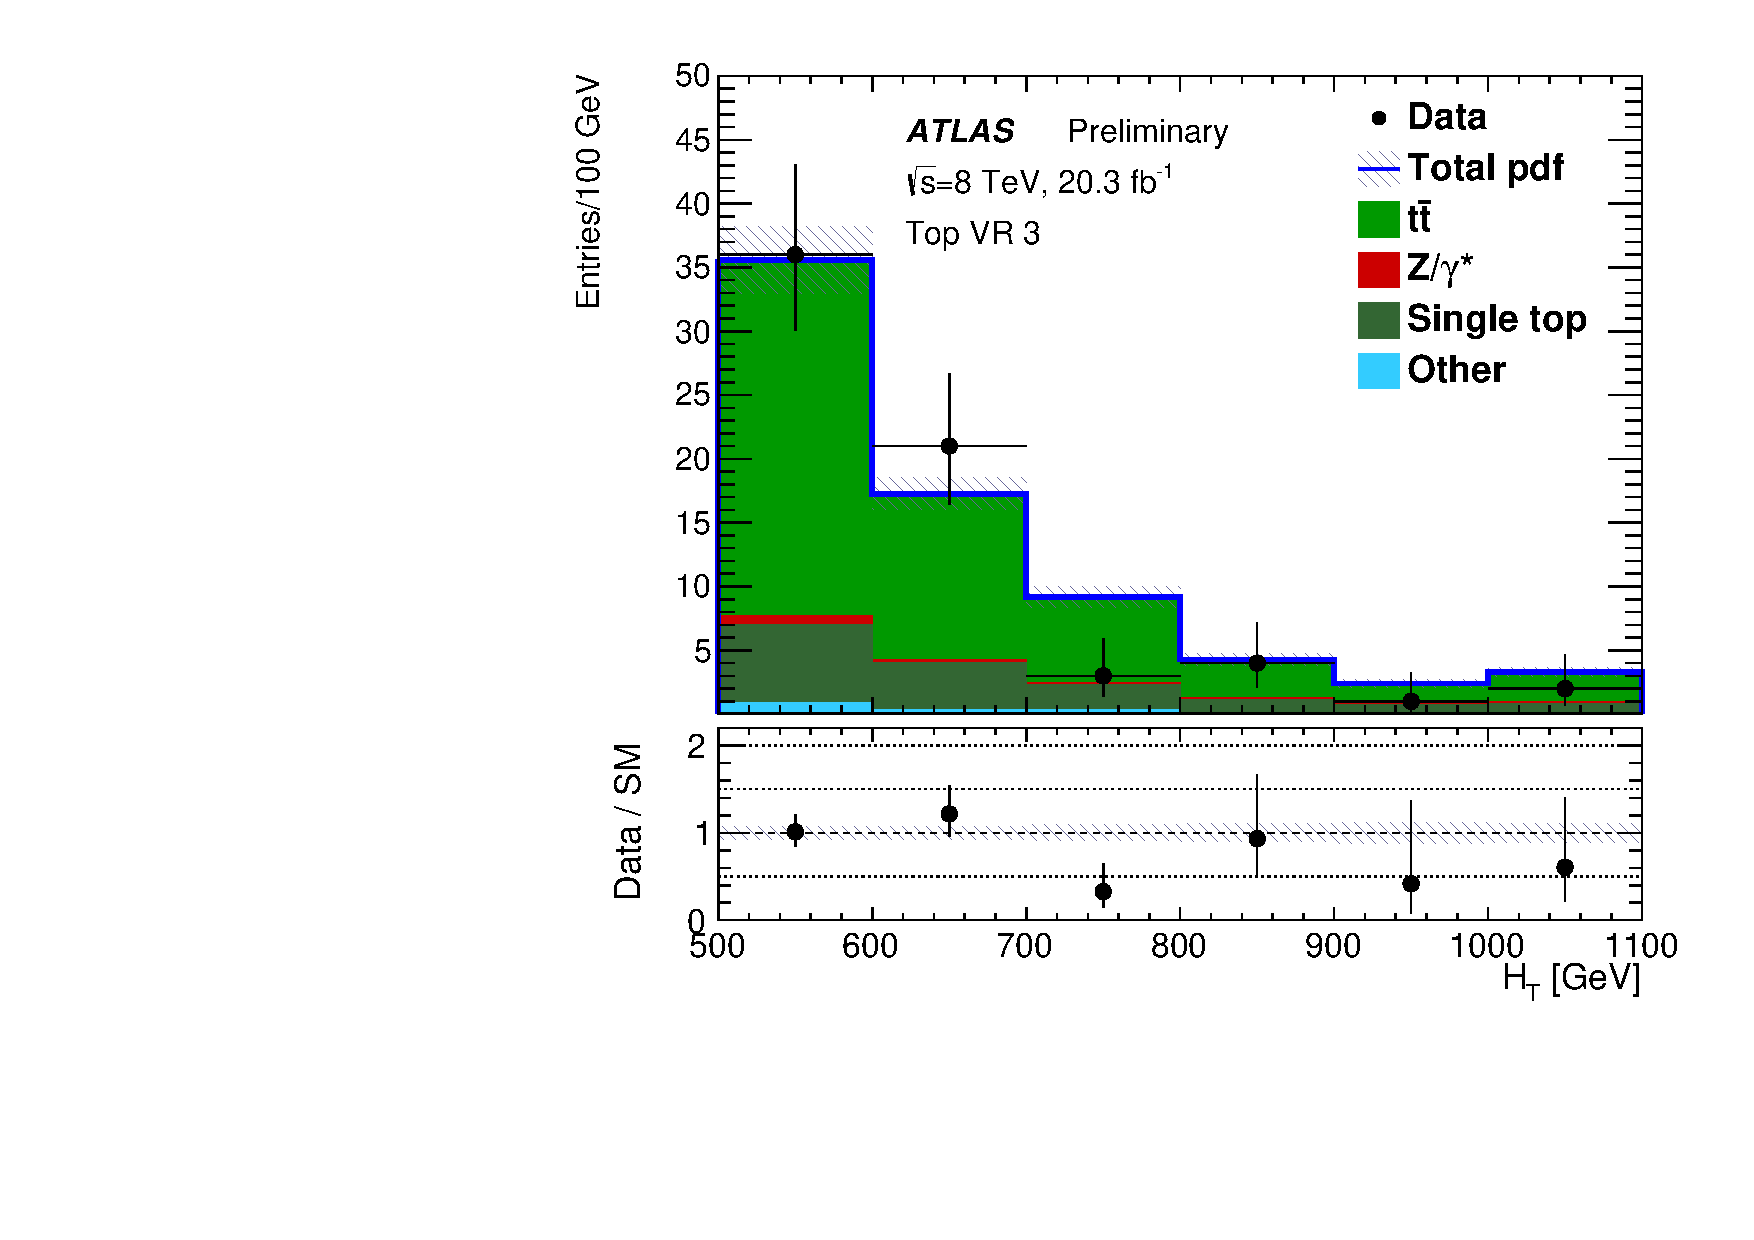
\includegraphics[width=0.48\textwidth]{figs/blstop/vr_top_3_ht_signal.pdf}
  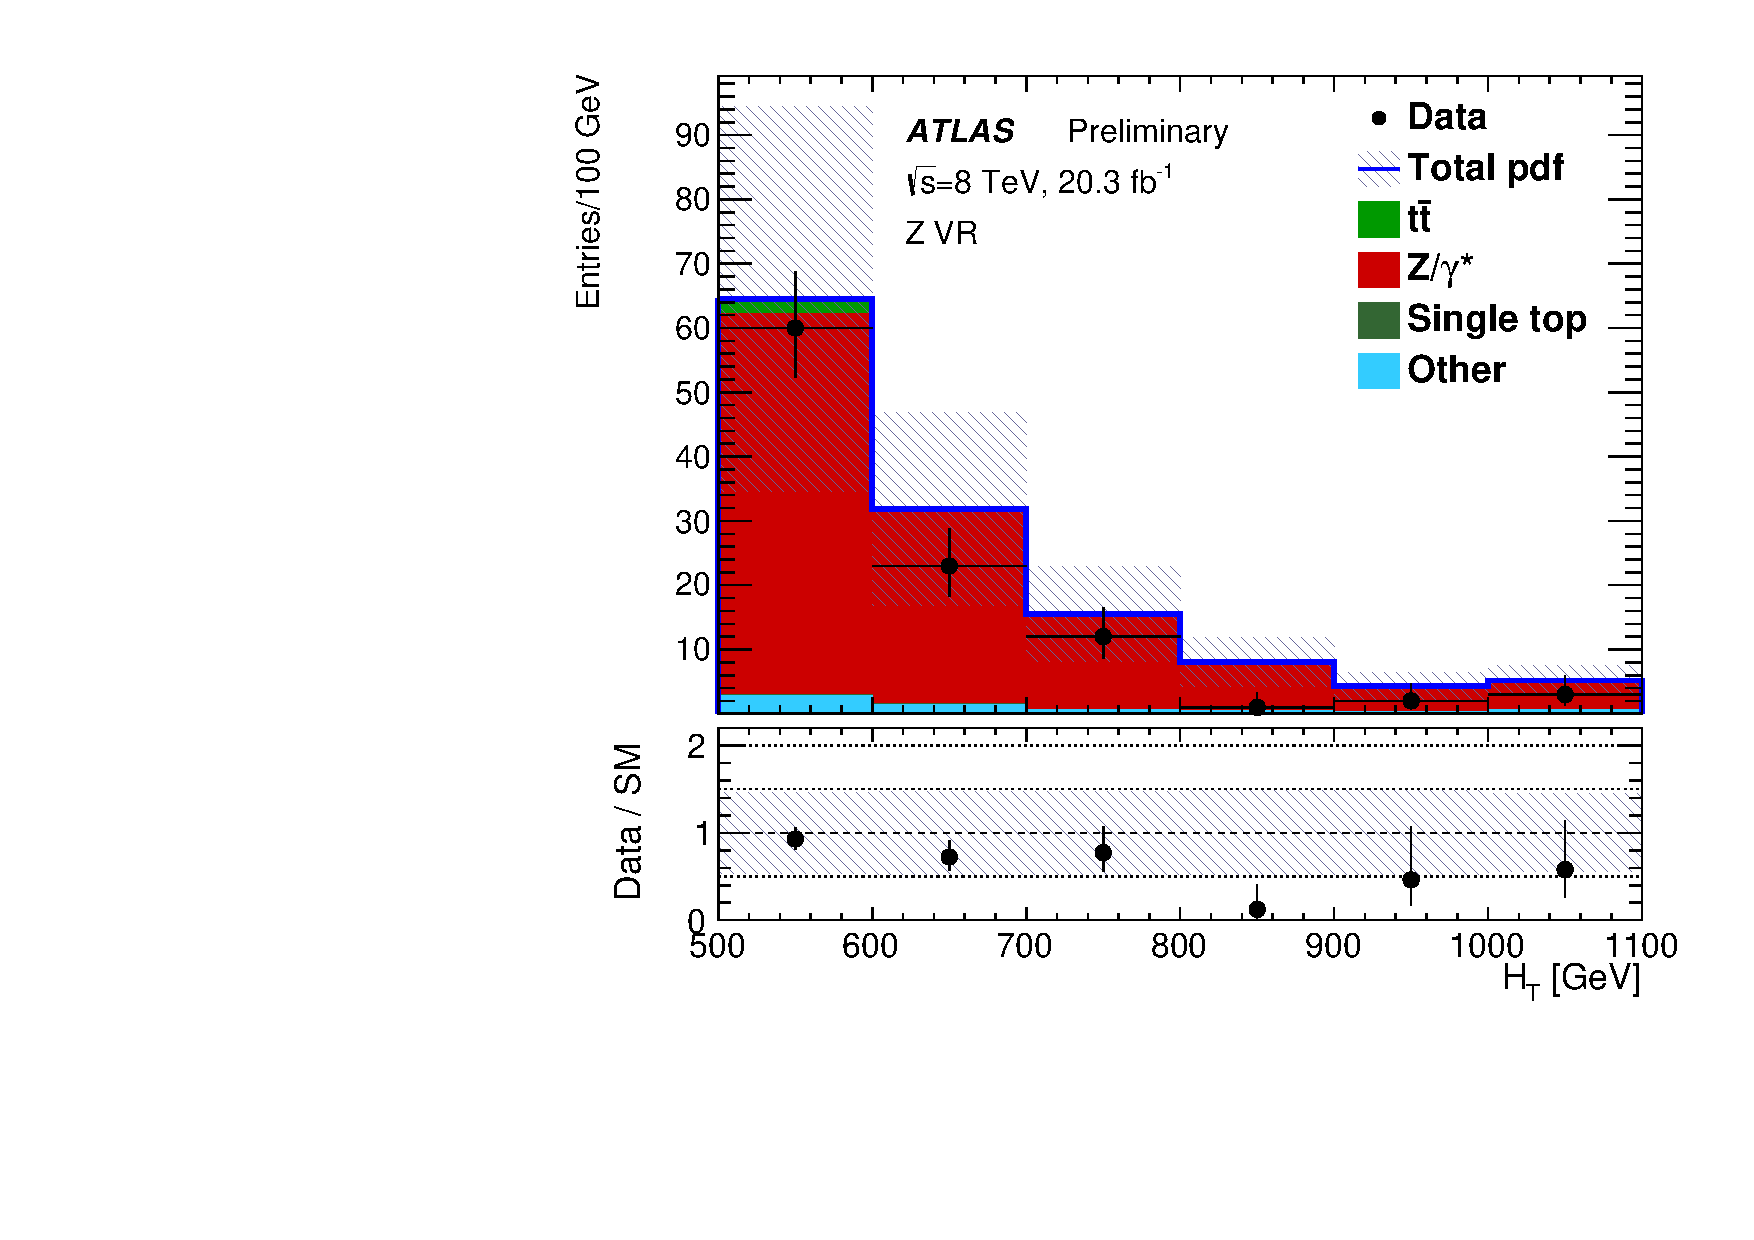
\includegraphics[width=0.48\textwidth]{figs/blstop/vr_Z_ht_signal.pdf}
  \caption{The \HT\ distribution in Top VR 3 (left) and $Z$ VR (right).
    The Standard Model background prediction is shown after setting the
    normalization of the \TTBAR\ and \ZGAMMAJETS\ backgrounds based on the
    observed data in the CRs.
    The hashed bands show the uncertainty on the fitted background prediction
    including all statistical and systematics uncertainties.
    The bottom of each plot shows the ratio of the observed data to the
    Standard Model background prediction.
  }
  \label{fig:ht_vr}
\end{figure}


%% -----------------------------------------------------------------------------
\FloatBarrier
\section{Systematic uncertainties}
\label{sec:systematics}

In addition to the statistical uncertainty, several sources of systematic
uncertainty are considered when determining the estimated signal and background
contributions.
The largest sources of systematic uncertainty are those related to the
MC statistical uncertainty in the SRs, the JES, the $b$-tagging efficiency
The uncertainty on the lepton energy scale and resolution was considered,
but shown to be negligible.

%% - - - - - - - - - - - - - - - - - - - - - - - - - - - - - - - - - - - - - - -
The uncertainty on the jet energy scale (JES) has an impact on both the jet
selection criteria and the kinematics of the event, such as the \HT\ and the
\MET\ measurements.
The JES uncertainty is evaluated using the EM+JES scheme as described
in~\cite{JES}, and the scaling is provided by the
\texttt{MultijetJESUncertaintyProvider} tool.
The uncertainty on the JES is composed of 16 parameters, and takes into account
the dependence on \pt, $\eta$, jet flavor, and the number of primary vertices.
The effect of each component on the event yield is estimated by varying the
component by $\pm 1 \sigma$ in the MC simulation and re-running the full event
selection, propagating the variation in the JES to the jet selection and related
kinematic quantities.

%% - - - - - - - - - - - - - - - - - - - - - - - - - - - - - - - - - - - - - - -
The uncertainty on the jet energy resolution (JER) is evaluated by applying an
additional smearing to the \pt\ measurement of each of the jets in the MC
simulation.
The size of the smearing is determined in dijet events as described
in~\cite{JER}.
The smearing is provided by the \texttt{JetSmearingTool} tool, and depends on
the \pt\ and \eta\ of the jets within an event.
The JER smearing alters the \pt\ of the jets within the event, and therefore
the event selection.
As with the JES, the JER uncertainty is evaluated by re-running the full event
selection on MC simulation, applying the smearing, then propagating the
variations to the event kinematic variables and yields.

%% - - - - - - - - - - - - - - - - - - - - - - - - - - - - - - - - - - - - - - -
As flavor tagging is used in this analysis, the efficiency of the $b$-tagging
algorithms affects the overall yields in each of the analysis regions.
This includes the possibility of a light flavor jet being incorrectly tagged
as a $b$-jet, or a jet which initiated by a $b$-quark failing the $b$-tagging
requirement.
The $b$-tagging efficiency uncertainty is broken into three components,
corresponding to the tagging and rejection efficiency of the different jet
flavors, $b$-jets, $c$-jets, and light flavor jets (light quarks and gluons).
These uncertainties take into account the dependence on \pt\ and jet flavor.
For the MC simulation, the $b$-tagging efficiency is implemented as a scale
factor, so the $b$-tagging uncertainty can be evaluated without running the
full event selection multiple times.
Rather, the $b$-tagging scale factor is varied up or down based on the specific
parameter of interest, and used to determine the uncertainty on the event yield.

%% - - - - - - - - - - - - - - - - - - - - - - - - - - - - - - - - - - - - - - -
The backgrounds are constrained in the CRs which are regions with low \HT,
while the SRs require high \HT.
Top VR 3 and $Z$ VR are used to assess any uncertainty associated with the
extrapolation from low \HT\ to high \HT.
The \TTBAR\ background extrapolation is assessed using Top VR 3. It can be seen
from Table \ref{tab:bkg_only_fit_results} that the post-fit background estimate
in Top VR 3 is in reasonably agreement with the observed data, so no additional
uncertainty is applied to the \TTBAR\ backgrounds due to the \HT\ extrapolation.
The \ZGAMMAJETS\ background extrapolation is assessed using the $Z$ VR.
The overall background is overpredicted in this region by 29\%, and the
prediction is the worst in the highest \HT\ bins.
An additional uncertainty of 50\% is applied to the \ZGAMMAJETS\ background
for events with $\HT > 500 GeV$.
% An \HT\ extrapolation uncertainty of 50\% is applied to \ZGAMMAJETS\ events
% with $\HT \geq 500$~\GeV. This is assigned to account for uncertainty on
% the \ZGAMMAJETS\ \HT\ spectrum. This uncertainty is derived from the
% disagreement observed in Figures~\ref{fig:pull_dist_vr}-\ref{fig:ht_vr}.
%%

%% - - - - - - - - - - - - - - - - - - - - - - - - - - - - - - - - - - - - - - -
Several theoretical uncertainties are considered in the modeling of the major
background processes in MC simulation.
These include the uncertainty on the cross sections, scale variations, and
generator uncertainties.
These uncertainties are evaluated by performing the event selection using only
the MC truth information, and comparing the expected event yields obtained
from MC simulation samples produced using different generator configurations.
An additional systematic uncertainty, due to the $\pm 2.8$\% uncertainty on the
integrated luminosity is evaluated for all background processes except
\TTBAR\ and \ZGAMMAJETS, because these backgrounds take the normalization from
data control regions.
A breakdown of the estimated effect of each source of systematic uncertainty
(both experimental and theoretical) are outlined in
Table~\ref{tab:systematic_breakdown}.

%% - - - - - - - - - - - - - - - - - - - - - - - - - - - - - - - - - - - - - - -
%% ttbar theory systematics
The sources of systematic uncertainty specific to the \TTBAR\ background include
the renormalization and factorization scale variations, MC generator
uncertainties, parton shower, and the amount of initial or final state
radiation (ISR or FSR) in the event.
%%
% scale variations
The scale variations are evaluated by comparing the expected event yields at the
truth level obtained using dedicated \TTBAR\ samples, each generated using
\powheg\ and \pythia, where the factorization and renormalization
scales are varied up and down by a factor of 2.
This isolates the effect of each of the scale variations, and the difference in
expected number of events in each region is taken to be the uncertainty on the
\TTBAR\ background.
The differences in the expected event yields for these samples is take to be
the uncertainty due to the scale variations.
%%
% MC generator
The MC generator uncertainty accounts for the difference in the MC predictions
obtained using different generator programs.
These are assessed by comparing the truth level event selection for a
\TTBAR\ sample generated using \powheg\ and \jimmy\ with a sample
generated using \mcnlo\ and \jimmy.
Since \jimmy\ is used to perform the parton shower in both of these
samples, the differences can be attributed to the differences in the
generation rather than the parton shower step.

%%
% parton shower
The uncertainty in the parton shower in \TTBAR\ samples is estimated by
comparing the expected event yields using the truth level information for two
\TTBAR\ samples each generated using \powheg.
One sample uses \pythia\ for the parton shower step, while the other
uses \jimmy.
This isolates the parton shower part of the MC simulation, which is performed
either using \pythia\ or \jimmy.
%%
% ISR/FSR
The uncertainty on the ISR and FSR is evaluated by comparing the expected number
of events in a truth level event selection found in two \TTBAR\ samples, each
generated using \acermc\ and \pythia.
The two samples differ in the amount of parton shower is included in the
simulation.
%%

%% - - - - - - - - - - - - - - - - - - - - - - - - - - - - - - - - - - - - - - -
%% single top theory systematics
The sources of systematic uncertainty specific to the single top background
include the single top cross section, the MC generator uncertainties, the parton
shower, ISR and FSR, and the interference with \TTBAR.
%%
% cross section
Single top can be produced through three production channels, with production
cross sections
\begin{itemize}
  \item $s$-channel: $5.61 \pm 0.22$ pb
  \item $t$-channel: $87.76^{+3.44}_{-1.91}$ pb
  \item $Wt$-channel: $22.37 \pm 1.52$ pb.
\end{itemize}
It was shown that the $Wt$-channel is dominant single top production channel for
the regions of interest.
For his reason, the uncertainty on the $Wt$-channel cross section is the only
single top cross section uncertainty which is considered, and a systematic
uncertainty of 7\% was applied to the single top background estimate in every
analysis region.
%%
% MC gen uncertainty.
The MC generator uncertainty on the single top background estimate is evaluated
by comparing the predicted yields from two single top samples, one generated
using \powheg, and the other generated using \mcnlo.
Both MC samples use \herwig\ to calculate the parton shower.
%%
% parton shower
The parton shower uncertainty is determined by comparing the truth level yields
of two simulated $Wt$-channel samples, each generated using \herwig.
The parton shower step was performed using \pythia\ and \herwig.
%%
% ISR/FSR
Similar to the \TTBAR\ background, the uncertainty on the single top background
estimate due to ISR and FSR uncertainties is determined by comparing two
samples, each generated using \acermc\ and \pythia, where the two samples
differ in the amount of parton shower is included in the simulation
%%
% ttbar interference
There is some interference between the \TTBAR\ and the $Wt$-channel single top
background processes.
This interference is handled by applying an additional uncertainty to the single
top background estimate by comparing the truth level event selection of two
$Wt$-channel samples, each generated using \powheg, but one using the DS
renormalization scheme, and the other using the DR renormalization scheme.

%% - - - - - - - - - - - - - - - - - - - - - - - - - - - - - - - - - - - - - - -
%% Z+jets theory systematics
In addition to the \HT\ extrapolation uncertainty discussed previously, an
additional uncertainty is applied to account for the finite number of partons in
the \ZGAMMAJETS\ background MC samples.
This uncertainty is evaluated by comparing the truth level event yields for two
\ZGAMMAJETS\ samples, generated with different numbers of additional partons
included in the matrix element calculation.
The first sample has exactly four additional partons in the matrix element
calculation, while the second set has four or five additional partons.
Both samples are generated using \sherpa.

%% - - - - - - - - - - - - - - - - - - - - - - - - - - - - - - - - - - - - - - -
%% MC stat systematics
In addition to the above sources of systematic uncertainty, the uncertainty
on the background estimate due to limited MC statistics in the CRs and SRs is
considered.
The MC statistical uncertainty was evaluated for each background process
independently in each analysis region as
\begin{equation}
  \sigma_{r,p}^\mathrm{MC~stat}
  =
  \sqrt{N_{r,p}^\mathrm{gen}},
\end{equation}
where $r$ and $p$ represent the region and background MC process respectively.
$N_{r,p}^\mathrm{gen}$ is the number of MC simulated events from background
process $p$ in region $r$.
No weights or scale factors are applied to this number of simulated events.
The total relative uncertainty in a region $r$ due to MC statistical
limitations ($\sigma_{r}^\mathrm{MC~stat,relative}$) is obtained by summing the
relative uncertainties for each process in region $r$ in quadrature, giving
\begin{equation}
  \sigma_{r}^\mathrm{MC~stat,relative}
  =
  \sqrt{ \sum_{p} \left(\frac{\sigma_{r,p}^\mathrm{MC~stat}}{N_{r,p}^\mathrm{gen}}\right)^2 }
  =
  \sqrt{ \sum_{p} \frac{1}{N_{r,p}^\mathrm{gen}} }.
\end{equation}
The total MC statistical uncertainty is evaluated in each region, and treated
as a systematic uncertainty on the background estimate.
The Top CR and $Z$ CR are used to constrain the \TTBAR\ and
\ZGAMMAJETS\ background estimates, so the MC statistical uncertainty in the
CRs results in additional uncertainty on the background estimate in the SRs.
For this reason, the MC statistical uncertainty in the Top ($Z$) CR is applied
as an additional systematic uncertainty on the \TTBAR\ (\ZGAMMAJETS) background
estimate in the SRs.

%% - - - - - - - - - - - - - - - - - - - - - - - - - - - - - - - - - - - - - - -
\begin{table}[ht]
\caption{Summary of the effect of each considered sources of systematic
  uncertainty on the background estimate in SR~400 and SR~600. Several
  sources of theoretical systematic uncertainty which have a small
  effect on the total background estimate are grouped into the
  ``Other theory'' category.
  {\color{red} TODO update this table with broken down info and CRs.}
}
\label{tab:systematic_breakdown}
%
\centering{
  \begin{tabular}{lcc}
  \toprule
    Systematic &
    \multirow{2}{*}{SR~400} &
    \multirow{2}{*}{SR~600} \\
    Uncertainty (\%) \\
    \midrule
    JES                          & 15     & 3  \\
    $b$-tagging                  & 13     & 12 \\
    JER                          & 5      & 1  \\
    Luminosity                   & 1      & 1  \\
    \midrule                                   
    \HT\ extrapolation           & 19     & 20 \\
    MC statistical               & 13     & 23 \\
    CR statistical               & 3      & 3 \\
    $Wt$ cross section           & 2      & 2  \\
    Other theory                 & 1      & 2  \\
    \bottomrule
    \end{tabular}
}
\end{table}

When determining the expected contributions of each of the signal models,
the effects of the JES, $b$-tagging efficiency, JER, and luminosity are
considered as well as the uncertainty on the signal model cross section,
outlined in Table~\ref{tab:stop_xsec}.

%% -----------------------------------------------------------------------------
\FloatBarrier
\section{Results}
\label{sec:results}

The background yields in the signal regions are determined using a maximum
likelihood fit~\cite{Baak:2014wma} for the \TTBAR\ and
\ZGAMMAJETS\ normalizations, which are constrained by the observed data in the
Top and $Z$ CRs.
The systematic uncertainties described previously are included as
Gaussian-distributed nuisance parameters.
The fitted background yields and the observed number of events in each
signal region are shown in Tables~\ref{tab:event_yields_sr_400} and
\ref{tab:event_yields_sr_600}.
Two events are observed, in agreement with the Standard Model prediction.
The kinematics of the two selected events are shown in
Table~\ref{tab:sr_event_kinematics}, the $\MBL^0$ and \HT\ distributions in
SR 400 are shown in Figure~\ref{fig:sr_dists}.
Event displays of the two events are shown in Figure~\ref{fig:event_displays}.

\begin{table}
  \caption{The expected and observed event yields in SR~400. The expected event
    yields are shown before and after performing the fit to the data in the
    control regions.
    The last three rows show the model-independent 95\% CL on
    the visible cross section and the number of events (expected and observed)
    in SR~400 from a generic non-Standard Model process.
  }
  \label{tab:event_yields_sr_400}
  %
  \begin{center}
    \begin{tabular}{lrrrr}
      \toprule
                                     & SR~400                & SR~400 $ee$           & SR~400 $\mu\mu$       & SR~400 $e\mu$  \\
      \midrule
      Observed                       & $2$                   & $0$                   & $2$                   & $0$                \\
      \midrule
      Fitted background              & $1.39 \pm 0.35$       & $0.36 \pm 0.15$       & $0.57 \pm 0.20$       & $0.45 \pm 0.11$    \\
      \midrule
      Fitted \TTBAR                  & $0.33 \pm 0.09$       & $0.07 \pm 0.08$       & $0.07 \pm 0.02$       & $0.19 \pm 0.05$    \\
      Fitted \ZGAMMAJETS             & $0.54 \pm 0.28$       & $0.20 \pm 0.10$       & $0.35 \pm 0.18$       & $\leq 0.01$    \\
      Single Top                     & $0.44 \pm 0.08$       & $0.10 \pm 0.03$       & $0.11 \pm 0.03$       & $0.23 \pm 0.05$    \\
      Other                          & $0.07 \pm 0.04$       & $\leq 0.01$           & $0.04 \pm 0.02$       & $0.03 \pm 0.03$    \\
      \midrule
      Input SM                       & $1.2$                 & $0.30$                & $0.46$                & $0.43$             \\
      \midrule
      Input \TTBAR                   & $0.30$                & $0.06$                & $0.06$                & $0.17$             \\
      Input \ZGAMMAJETS              & $0.38$                & $0.14$                & $0.24$                & $0.00$             \\
      Input single Top               & $0.44$                & $0.10$                & $0.11$                & $0.23$             \\
      Input other                    & $0.07$                & $0.00$                & $0.04$                & $0.03$             \\
      \midrule
      $\sigma_\mathrm{vis}$~[fb]     & $0.23$                & $0.11$                & $0.26$                & $0.11$                \\
      Observed $N_\mathrm{non-SM}$   & $4.8$                 & $2.2$                 & $5.4$                 & $2.3$                 \\
      Expected $N_\mathrm{non-SM}$   & ${4.0}^{+2.2}_{-1.1}$ & ${3.2}^{+1.7}_{-1.1}$ & ${3.6}^{+1.9}_{-1.5}$ & ${3.3}^{+1.8}_{-1.3}$ \\
      \bottomrule
    \end{tabular}
  \end{center}
\end{table}

\begin{table}
  \caption{The expected and observed event yields in SR~600. The expected event
    yields are shown before and after performing the fit to the data in the
    control regions.  The last three rows show the model-independent 95\% CL on
    the visible cross section and the number of events (expected and observed)
    in SR~600 from a generic non-Standard Model process.
  }
  \label{tab:event_yields_sr_600}
  %
  \begin{center}
    \begin{tabular}{lrrrr}
      \toprule
                                      & SR~600                & SR~600 $ee$           & SR~600 $\mu\mu$       & SR~600 $e\mu$   \\
      \midrule
      Observed                        & $1$                   & $0$                   & $1$                   & $0$              \\
      \midrule
      Fitted background               & $0.55 \pm 0.15$       & $0.15 \pm 0.06$       & $0.24 \pm 0.10$       & $0.16 \pm 0.06$  \\
      \midrule
      Fitted \TTBAR                   & $0.10 \pm 0.02$       & $0.03 \pm 0.01$       & $\leq 0.01$           & $0.07 \pm 0.03$  \\
      Fitted \ZGAMMAJETS              & $0.23 \pm 0.12$       & $0.08 \pm 0.05$       & $0.15 \pm 0.08$       & $\leq 0.01$  \\
      Single Top                      & $0.18 \pm 0.04$       & $0.03 \pm 0.01$       & $0.05 \pm 0.02$       & $0.09 \pm 0.03$  \\
      Other                           & $0.04 \pm 0.01$       & $\leq 0.01$           & $0.04 \pm 0.02$       & $\leq 0.01$  \\
      \midrule
      Input SM                        & $0.47$                & $0.12$                & $0.20$                & $0.16$           \\
      \midrule
      Input \TTBAR                    & $0.09$                & $0.03$                & $0.00$                & $0.06$           \\
      Input \ZGAMMAJETS               & $0.16$                & $0.06$                & $0.10$                & $0.00$           \\
      Input single Top                & $0.18$                & $0.03$                & $0.05$                & $0.09$           \\
      Input other                     & $0.04$                & $0.00$                & $0.04$                & $0.00$           \\
      \midrule
      $\sigma_\mathrm{vis}$~[fb]      & $0.19$                & $0.10$                & $0.20$                & $0.10$                \\
      Observed $N_\mathrm{non-SM}$    & $3.9$                 & $2.1$                 & $4.0$                 & $2.1$                 \\
      Expected $N_\mathrm{non-SM}$    & ${3.5}^{+1.9}_{-1.4}$ & ${2.6}^{+1.6}_{-0.6}$ & ${3.0}^{+1.7}_{-1.0}$ & ${2.7}^{+1.6}_{-0.7}$ \\
      \bottomrule
    \end{tabular}
  \end{center}
\end{table}

\begin{table}
  \caption{The event and object kinematics for the two events passing the
    signal region selection. The first event passes the SR~400 selection
    while the second event passes both SR~400 and SR~600 selections.
  }
  \label{tab:sr_event_kinematics}
  %
  \begin{center}
    \begin{tabular}{lcc}
      \toprule
      Run number              & 214216    & 210302  \\
      Event number            & 121272046 & 2292645861 \\
      \midrule
      $\MBL^0$ [\GeV]         & 558       & 686   \\
      %
      $\ell_0$ flavor         & $\mu$     & $\mu$ \\
      $\ell_0$ charge         & $-$       & $-$   \\
      %
      $\ell_0\ \pt$ [\GeV]    & 375       & 272   \\
      $b_0\ \pt$ [\GeV]       & 330       & 460   \\
      %
      $\ell_0\ \eta$          & $-0.11$   & 1.22  \\
      $b_0\ \eta$             & 0.56      & 0.95  \\
      %
      $\ell_0\ \phi$          & 2.0       & $-1.3$  \\
      $b_0\ \phi$             & $-2.7$    & 2.5   \\
      %
      \midrule
      $\MBL^1$ [\GeV]         & 526       & 528   \\
      %
      $\ell_1$ flavor         & $\mu$     & $\mu$ \\
      $\ell_1$ charge         & $+$       & $+$     \\
      %
      $\ell_1\ \pt$ [\GeV]    & 88        & 96    \\
      $b_1\ \pt$ [\GeV]       & 542       & 374   \\
      %
      $\ell_1\ \eta$          & 0.45      & 1.43  \\
      $b_1\ \eta$             & $-1.1$    & $-0.26$ \\
      %
      $\ell_1\ \phi$          & $-2.3$    & $-0.91$ \\
      $b_1\ \phi$             & $-0.21$   & 2.3   \\
      %
      \midrule
      \MBLASYM                & 0.03      & 0.13  \\
      \HT\ [\GeV]             & 1335      & 1203  \\
      \METSIG\ $[\GeV^{1/2}]$ & 2.9       & 6.4   \\
      \MET\ [\GeV]            & 107       & 223   \\
      $m_{\ell\ell}$ [\GeV]   & 324       & 71    \\
      \bottomrule
    \end{tabular}
  \end{center}
\end{table}

\begin{figure}[ht]
  \centering
  \subbottom[$\MBL^0$]{
    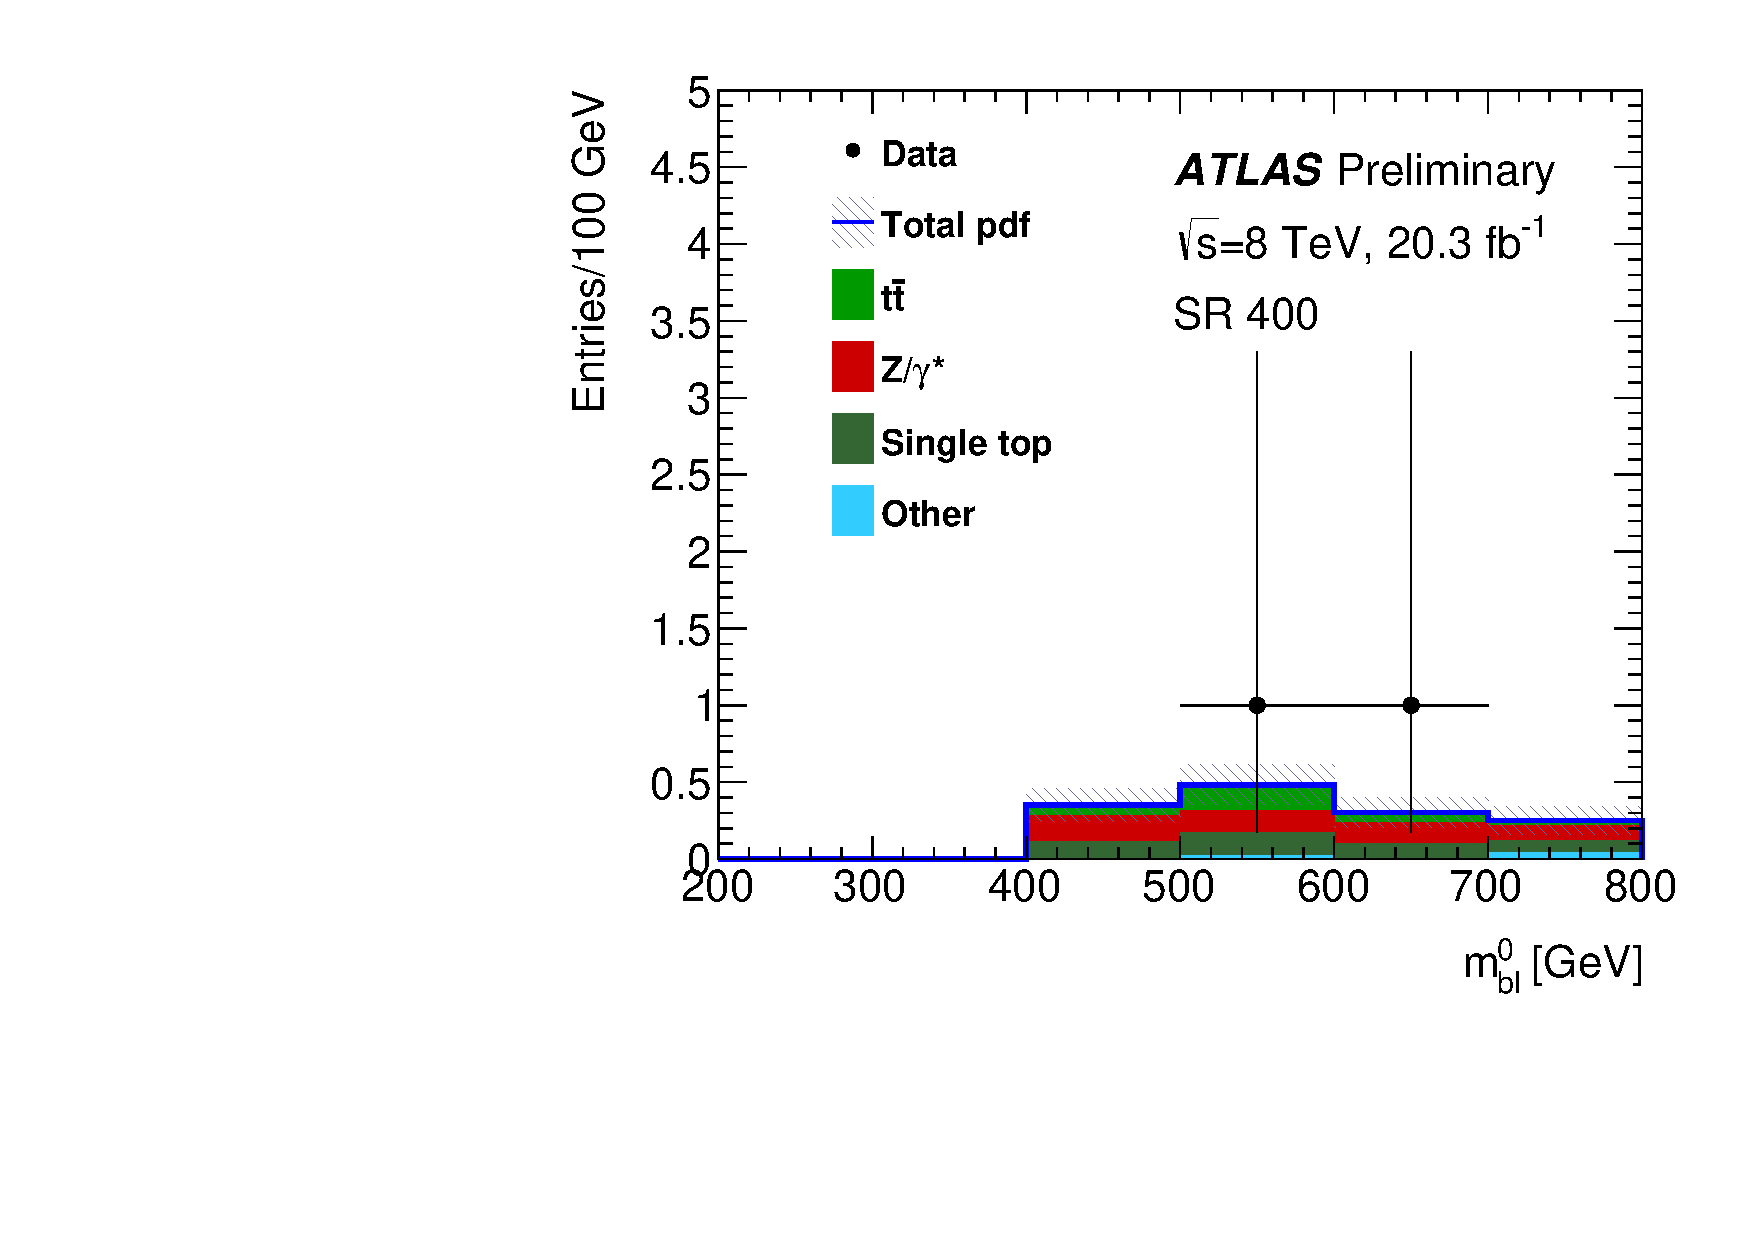
\includegraphics[width=0.45\textwidth]{figs/blstop/sr_mbl_0.pdf}
  }
  \subbottom[\HT]{
    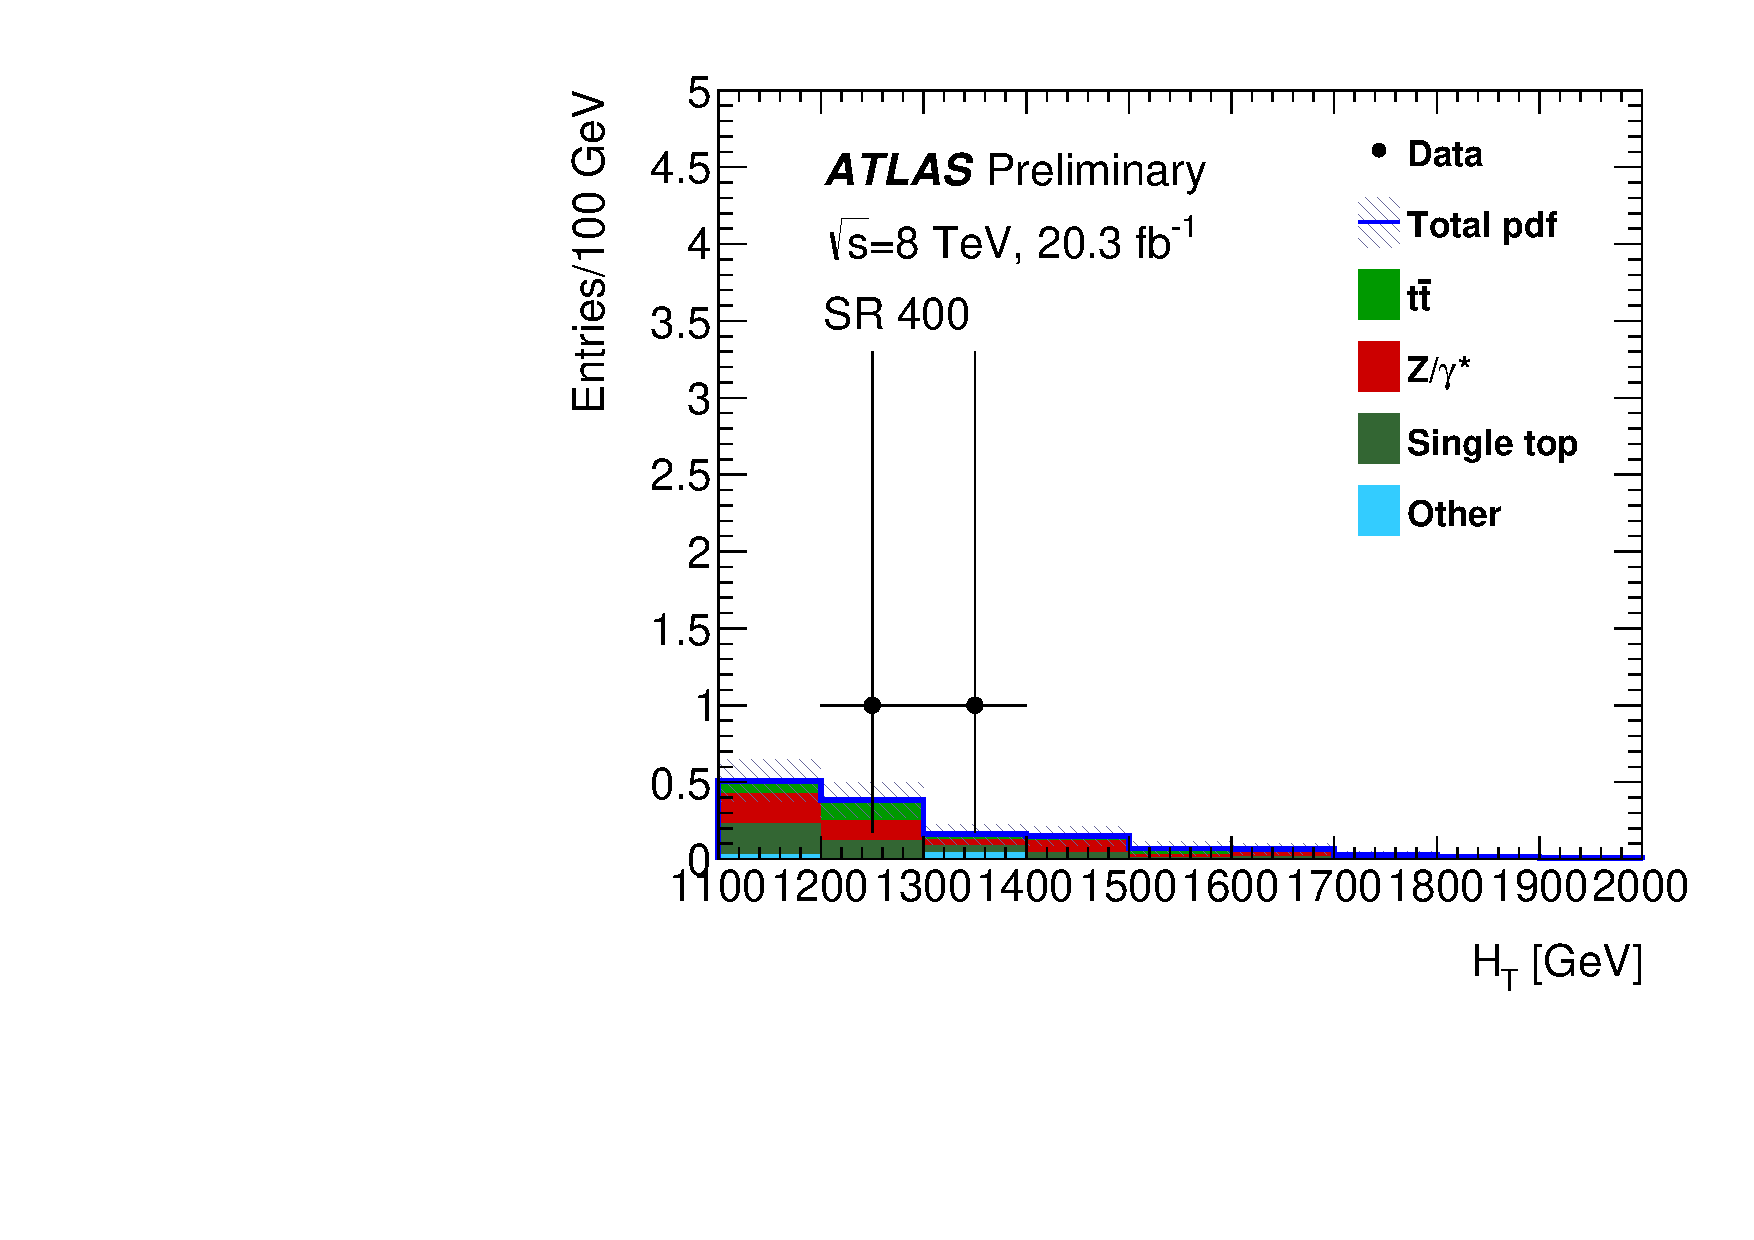
\includegraphics[width=0.45\textwidth]{figs/blstop/sr_ht.pdf}
  }
  \caption{These plots show the $\MBL^0$ (left) and \HT\ (right) distributions
    in SR 400. The Standard Model background prediction is taken from the
    fitted background prediction. The hashed bands show
    the uncertainty on the fitted background prediction including the MC
    statistical and sources of systematic uncertainty.  The bottom of
    each plot shows the ratio of the observed data to the Standard Model
    background prediction.
  }
  \label{fig:sr_dists}
\end{figure}

\begin{figure}[ht]
  \centering
  \subbottom[Run 214216, Event 121272046]{
    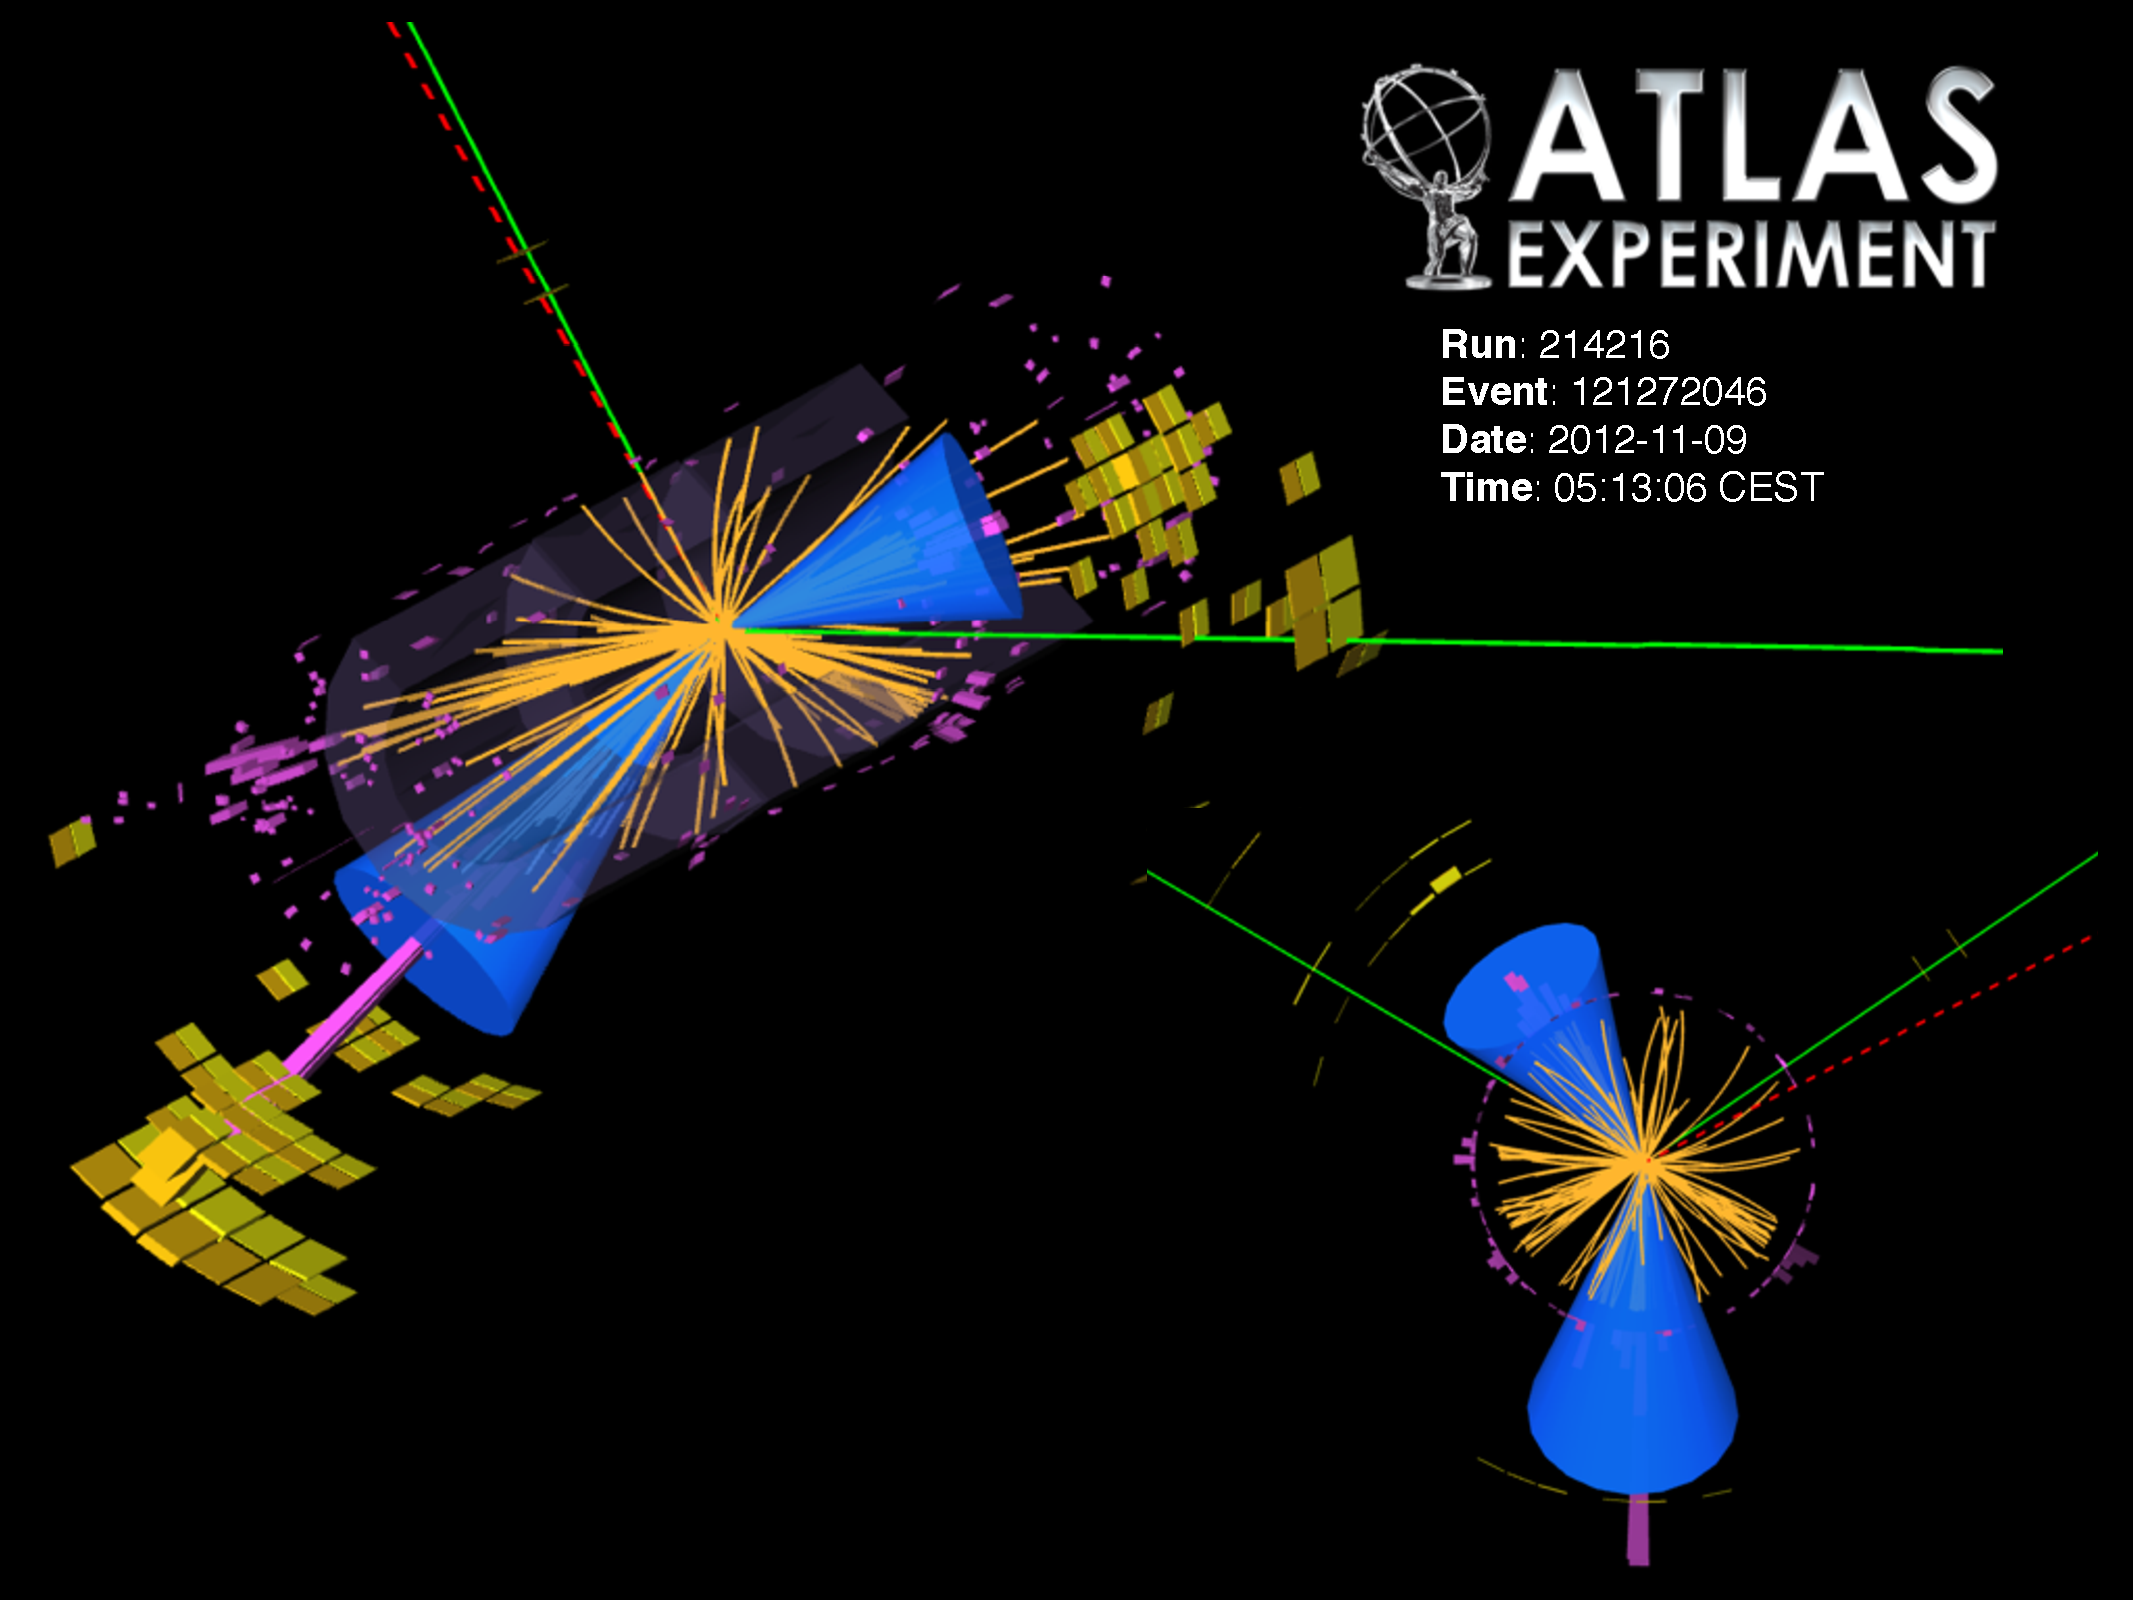
\includegraphics[height=0.41\textheight]
    {figs/blstop/event_display_run_214216_event_121272046.pdf}
    \label{fig:event_display_1}
  }
  \subbottom[Run 210302, Event 2292645761]{
    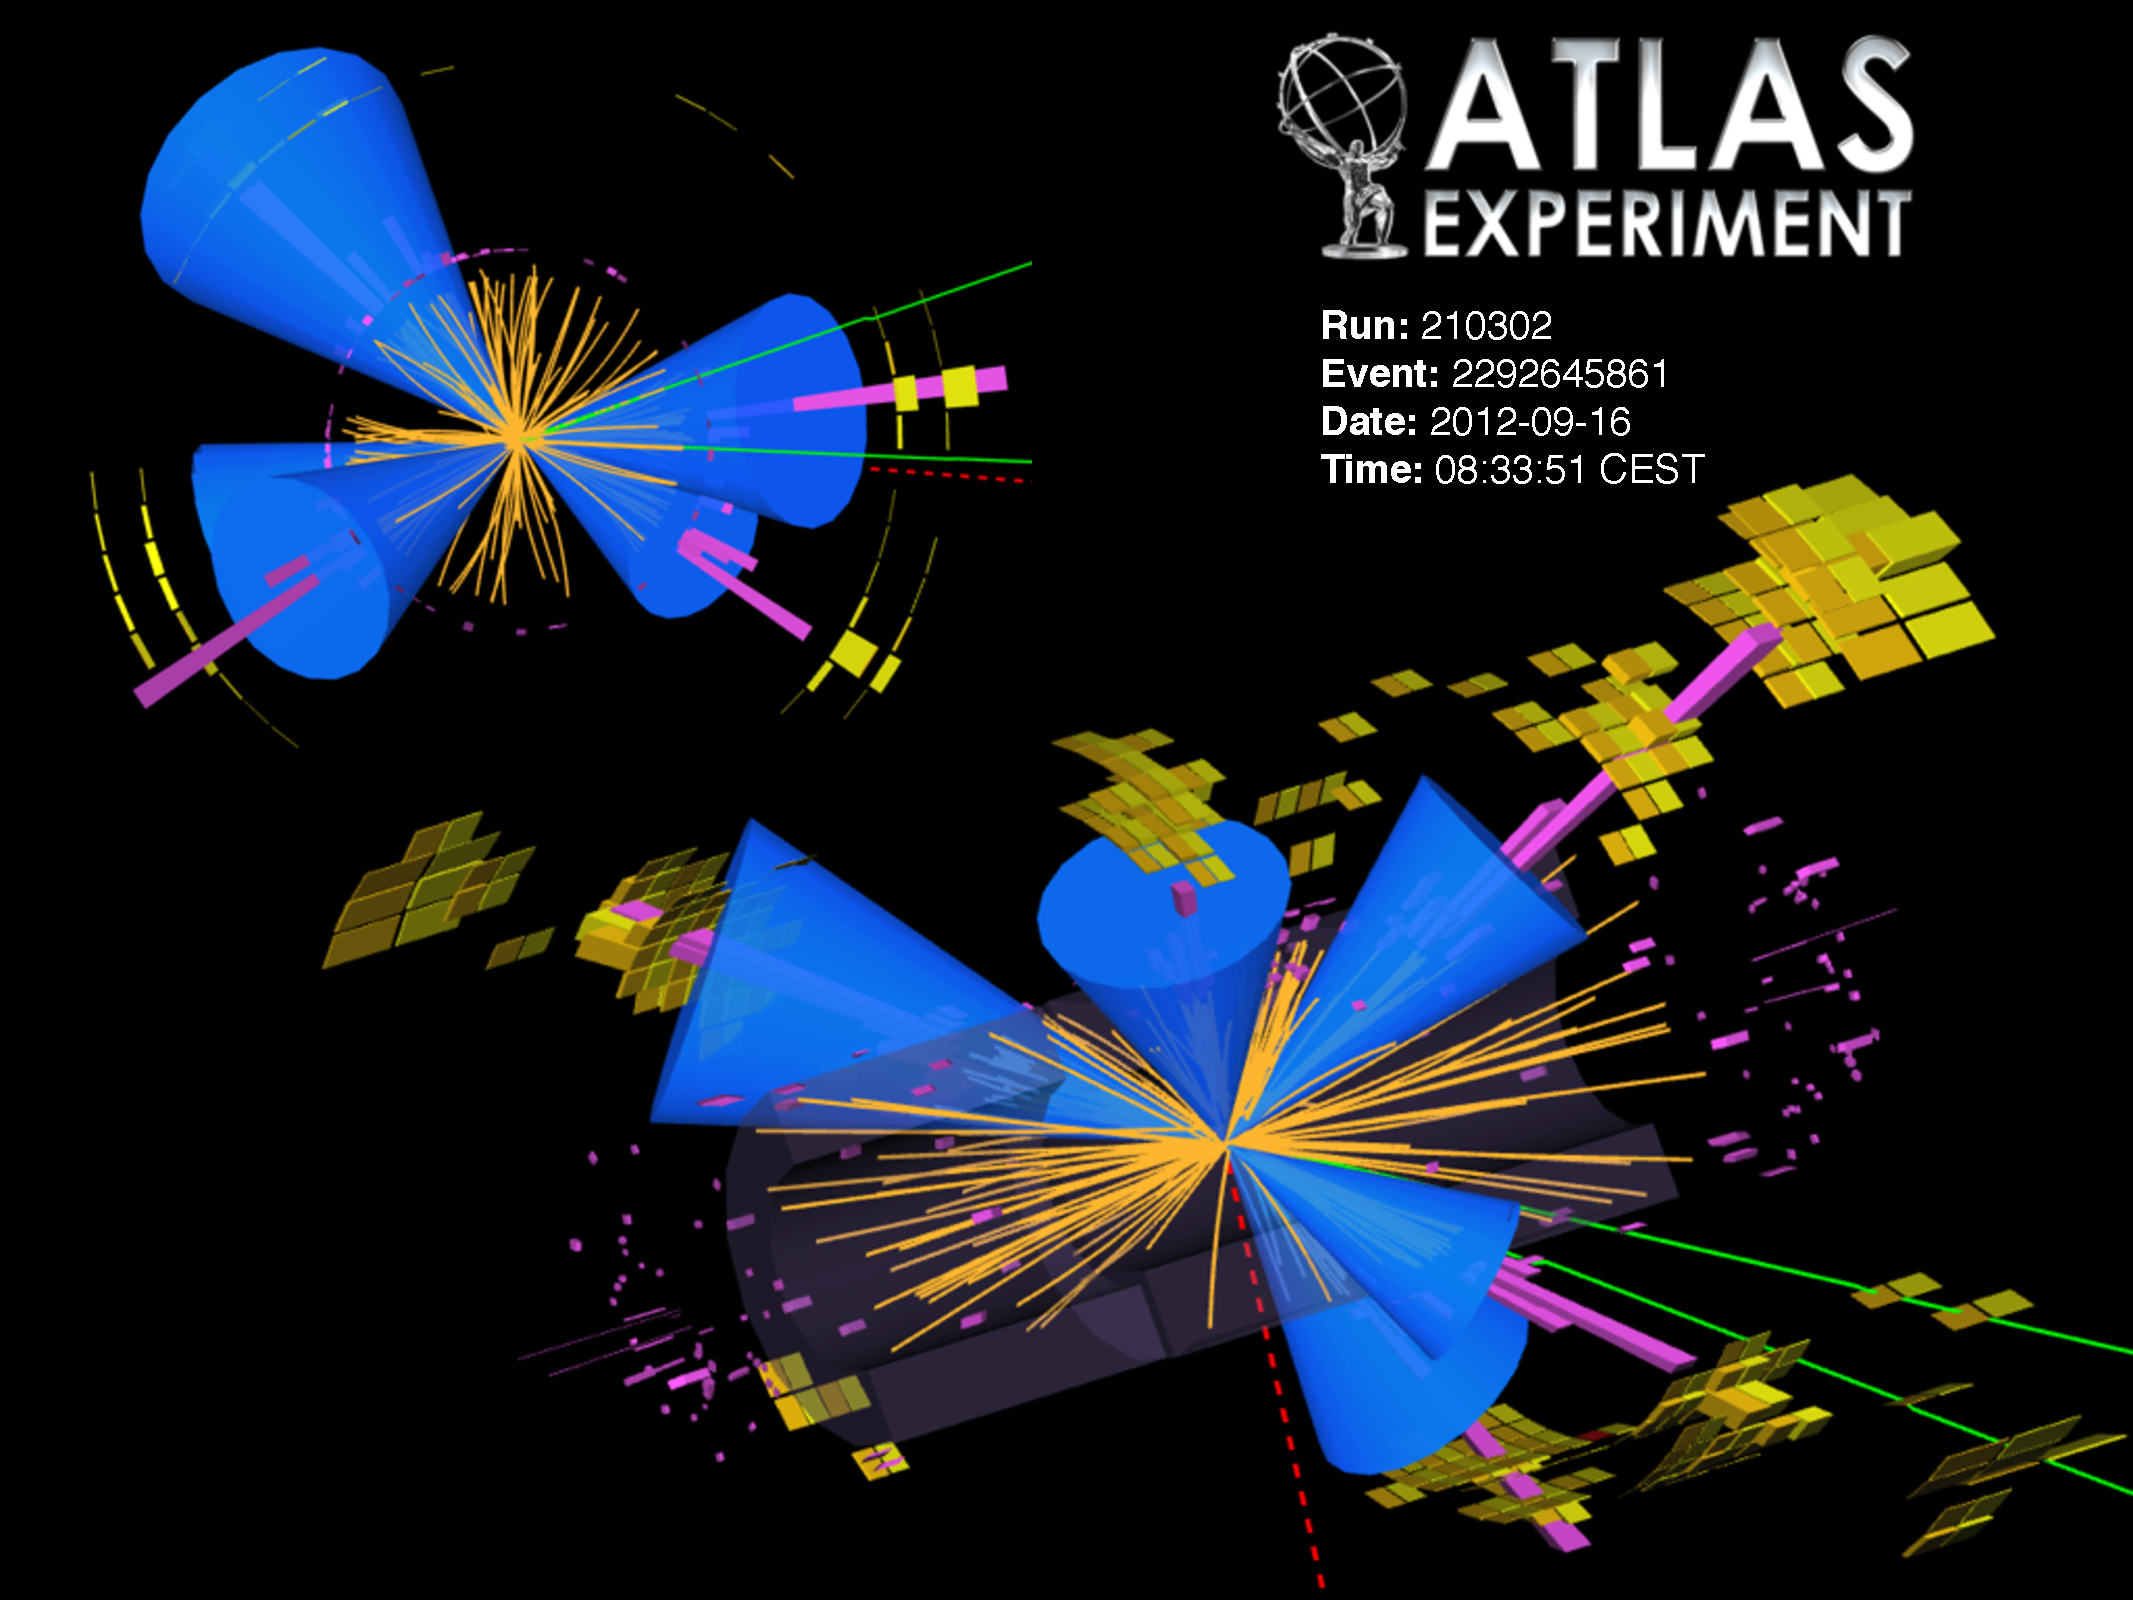
\includegraphics[height=0.41\textheight]
    {figs/blstop/event_display_run_210302_event_2292645761.pdf}
    \label{fig:event_display_2}
  }
  \caption{Event displays for the two observed events passing the signal region
    criteria.
    The event shown in Figure~\ref{fig:event_display_1} passes the SR~400
    selection with $\MBL^{0} = 558~\GeV$.
    Figure~\ref{fig:event_display_2} shows the event which passes both the
    SR~400 and SR~600 selection with $\MBL^{0} = 686~\GeV$.
  }
  \label{fig:event_displays}
\end{figure}

As the observed number of events is consistent with the Standard Model
prediction, Upper limits at 95\% confidence level (CL) on the number of
beyond the Standard Model (BSM) events for each signal region are derived
using the $CL_S$ prescription and neglecting any possible contamination in the
control regions~\cite{Baak:2014wma}.
Normalizing these by the integrated luminosity of the data sample they can be
interpreted as upper limits on the visible BSM cross section,
$\sigma_\mathrm{vis}$, where $\sigma_\mathrm{vis}$ is defined as the product of
acceptance, reconstruction efficiency and production cross section.
The model independent limits are given in
Tables~\ref{tab:event_yields_sr_400}~(SR 400)
and~\ref{tab:event_yields_sr_600}~(SR 600).

%% -----------------------------------------------------------------------------
\FloatBarrier
\subsection{Model dependent limits}
\label{sec:model_dependent_limits}

In the absence of an excess of events in the SRs beyond the SM prediction,
limits are set on the allowable stop masses and branching ratios for this model.
Expected and observed exclusion limits on the signal model are determined using
the $CL_S$ prescription based on a simultaneous fit of the SRs and
CRs~\cite{Baak:2014wma}.
The predicted signal contamination in the CRs is taken into account for each
signal model tested.
An expected and observed mass limit is first determined for a single choice of
stop branching ratio, $Br(\tilde{t} \to eb) = Br(\tilde{t} \to \mu b) = 0.5$,
the branching ratio simulated in the MC signal models.

Each SR (SR 400 and SR 600) is interpreted separately, using the predicted and
observed event yields in the CRs and the SR of interest.
A likelihood fit is performed to obtain the model-dependent estimate of the
background and signal strengths.
For the expected limit the data in the SR is replaced with the pre-fit MC
prediction.
An expected and observed $CL_S$ value is computed for each simulated stop mass,
in each SR to assess the relative compatibility of the data with the
signal~+~background hypothesis and the background only hypothesis.
For each stop mass, the SR which gives the best expected sensitivity, as
measured by the lower $CL_S$ value is selected, and used to interpret the model
at that mass.
The HistFitter package limits the precision of the $CL_S$ value to $10^{-6}$;
if the two SRs are affected by this cutoff, SR~400 is chosen by convention.
This simplification is not expected to affect the final result, as these points
are far from the mass limit boundary.
If the observed $CL_S$ value in the selected SR is less than 0.05, the signal
model is rejected at 95\%~CL, and an observed (expected) limit on the stop mass
is determined by taking the highest stop mass, with an observed (expected)
$CL_S$ value less than 0.05.
Figure~\ref{fig:exp_limit_br_5050} shows an example $CL_S$ plot (for both SRs)
for the scenario with $Br(\tilde{t} \to eb) = Br(\tilde{t} \to \mu b) = 0.5$.
In the high mass regime, SR~600 is selected to interpret the mode, and
the points where the solid line is below 0.05 (indicated with a dashed red line)
are excluded.
No interpolation between the mass points is performed, so the mass limit for
this choice of stop branching ratios is 900~\GeV.

\begin{figure}[t]
  \centering
  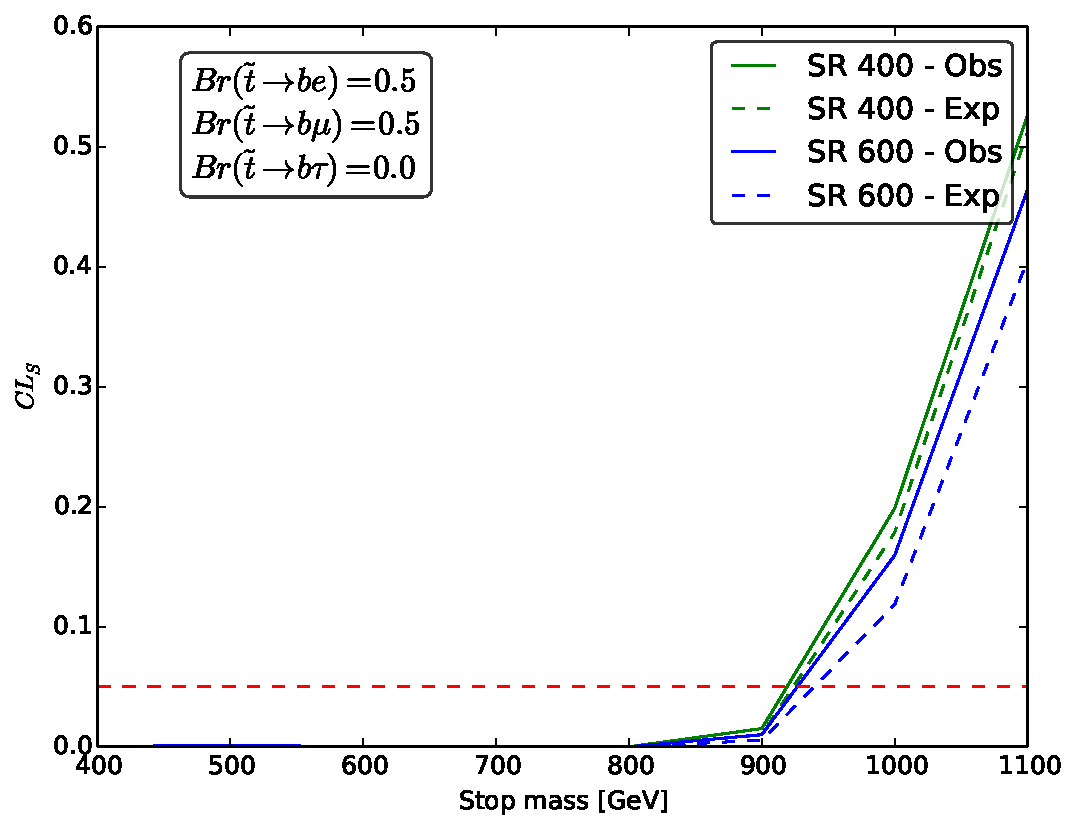
\includegraphics[width=0.75\textwidth]{figs/blstop/cls_plots/cls_vs_m_br_e_50_br_m_50_br_t_0.pdf}
  \caption{Expected and observed $CL_S$ value as a function of stop mass for
    the scenario with $Br(\tilde{t} \to eb) = Br(\tilde{t} \to \mu b) = 0.5$.
    The point where the line crosses $CL_S=0.05$ is where the expected limit is
    to be set.
  }
  \label{fig:exp_limit_br_5050}
\end{figure}

This procedure of finding a stop mass limit is repeated for branching ratios
across the plan of allowed values.
The MC simulation stop samples are generated with fixed branching
ratios ($Br(\tilde{t} \to eb) = Br(\tilde{t} \to \mu b) = 0.5$),
however, an additional event weight, dependent on the di-lepton flavor channel,
to scale the signal process to any desired choice of stop branching ratios.
It was shown that the disagreement between the generated and reconstructed
flavor channels is negligible, so the reconstructed di-lepton flavor channel
is used to select the additional weight.

The di-stop branching fractions are given by 
\begin{equation}
  \label{eqn:branching_fractions}
  \begin{aligned}
    Br_\mathrm{flavor}(\tilde{t}\tilde{t}^{*} \rightarrow bbee)     &=
      Br_\mathrm{flavor}(\tilde{t} \rightarrow be )^{2} \\
    Br_\mathrm{flavor}(\tilde{t}\tilde{t}^{*} \rightarrow bb\mu\mu) &=
      Br_\mathrm{flavor}(\tilde{t} \rightarrow b\mu )^{2} \\
    Br_\mathrm{flavor}(\tilde{t}\tilde{t}^{*} \rightarrow bbe\mu)   &=
      2Br_\mathrm{flavor}(\tilde{t} \rightarrow be )
      Br_\mathrm{flavor}(\tilde{t} \rightarrow b\mu ).
  \end{aligned}
\end{equation}

The di-stop branching fractions for each flavor channel are plotted for choices
of the single-stop branching ratio in Figure~\ref{fig:flavor_scaling_bf}, where
darker colors represent a higher branching fraction.
The simulated stop samples correspond the center of the $x$-axis, and have
di-stop branching fractions of 0.25, 0.25, and 0.50 for the $eebb$,
$\mu\mu bb$, $e\mu bb$ channels respectively.
As the value of $Br(\tilde{t} \to be)$ increases (represented by moving toward
the bottom right corner of each of the plots), the fraction of events decaying
to the $eebb$ final state increases, while the other two flavor channels
have fewer expected events.
Similarly, as the value of $Br(\tilde{t} \to b\mu)$ increases (represented by
moving toward the bottom left corner of each of the plots), the fraction of
events decaying to the $\mu\mu bb$ final state increases.
Finally, an increasing branching ratio of the $\tilde{t} \to b\tau$ decay
(represented by moving toward the upper left corner of the plots), the number
of expected events with two light leptons decreases.

\begin{figure}[ht]
  \centering
  \subbottom[Stop branching fractions for each flavor channel]{
    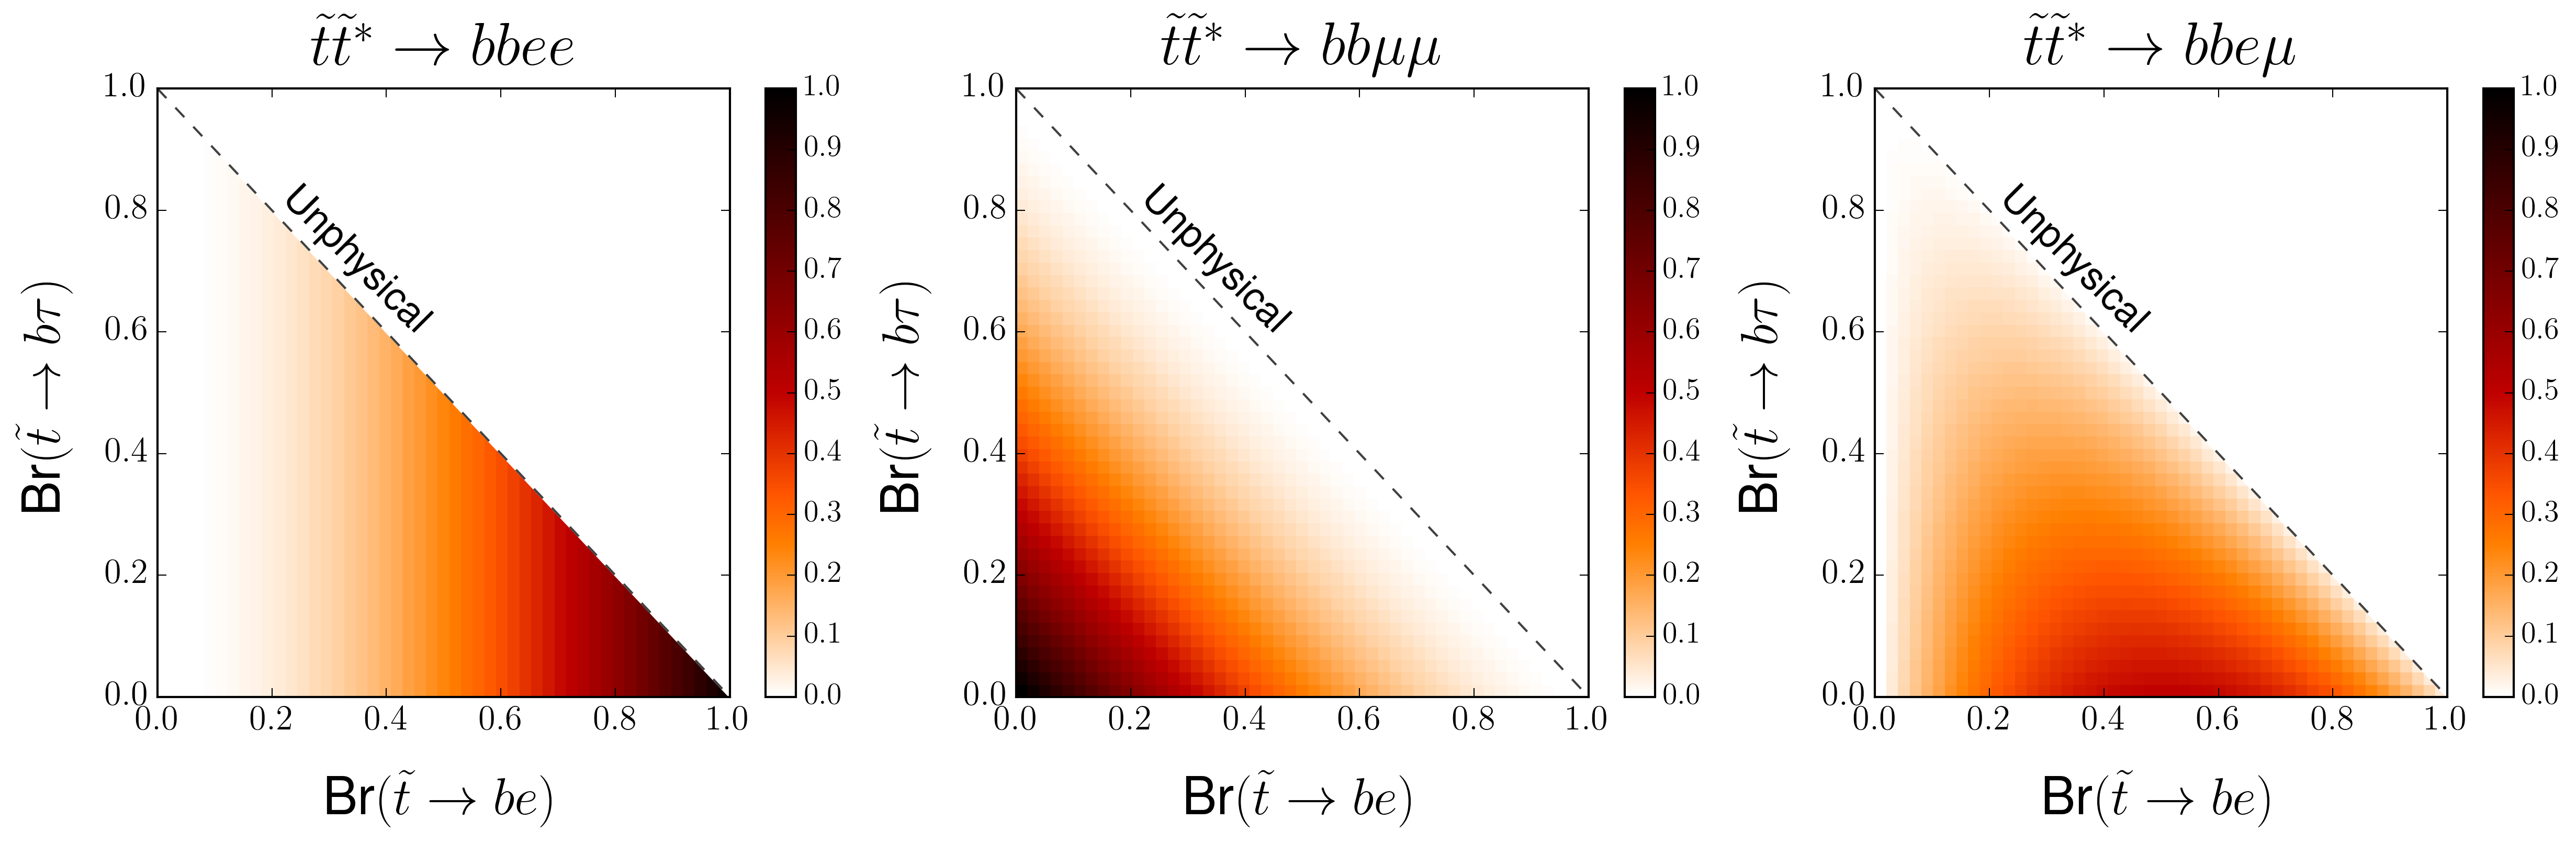
\includegraphics[width=\textwidth]{figs/blstop/branching_fractions.png}
    \label{fig:flavor_scaling_bf}
  }
  \subbottom[Scale factors for each flavor channel]{
    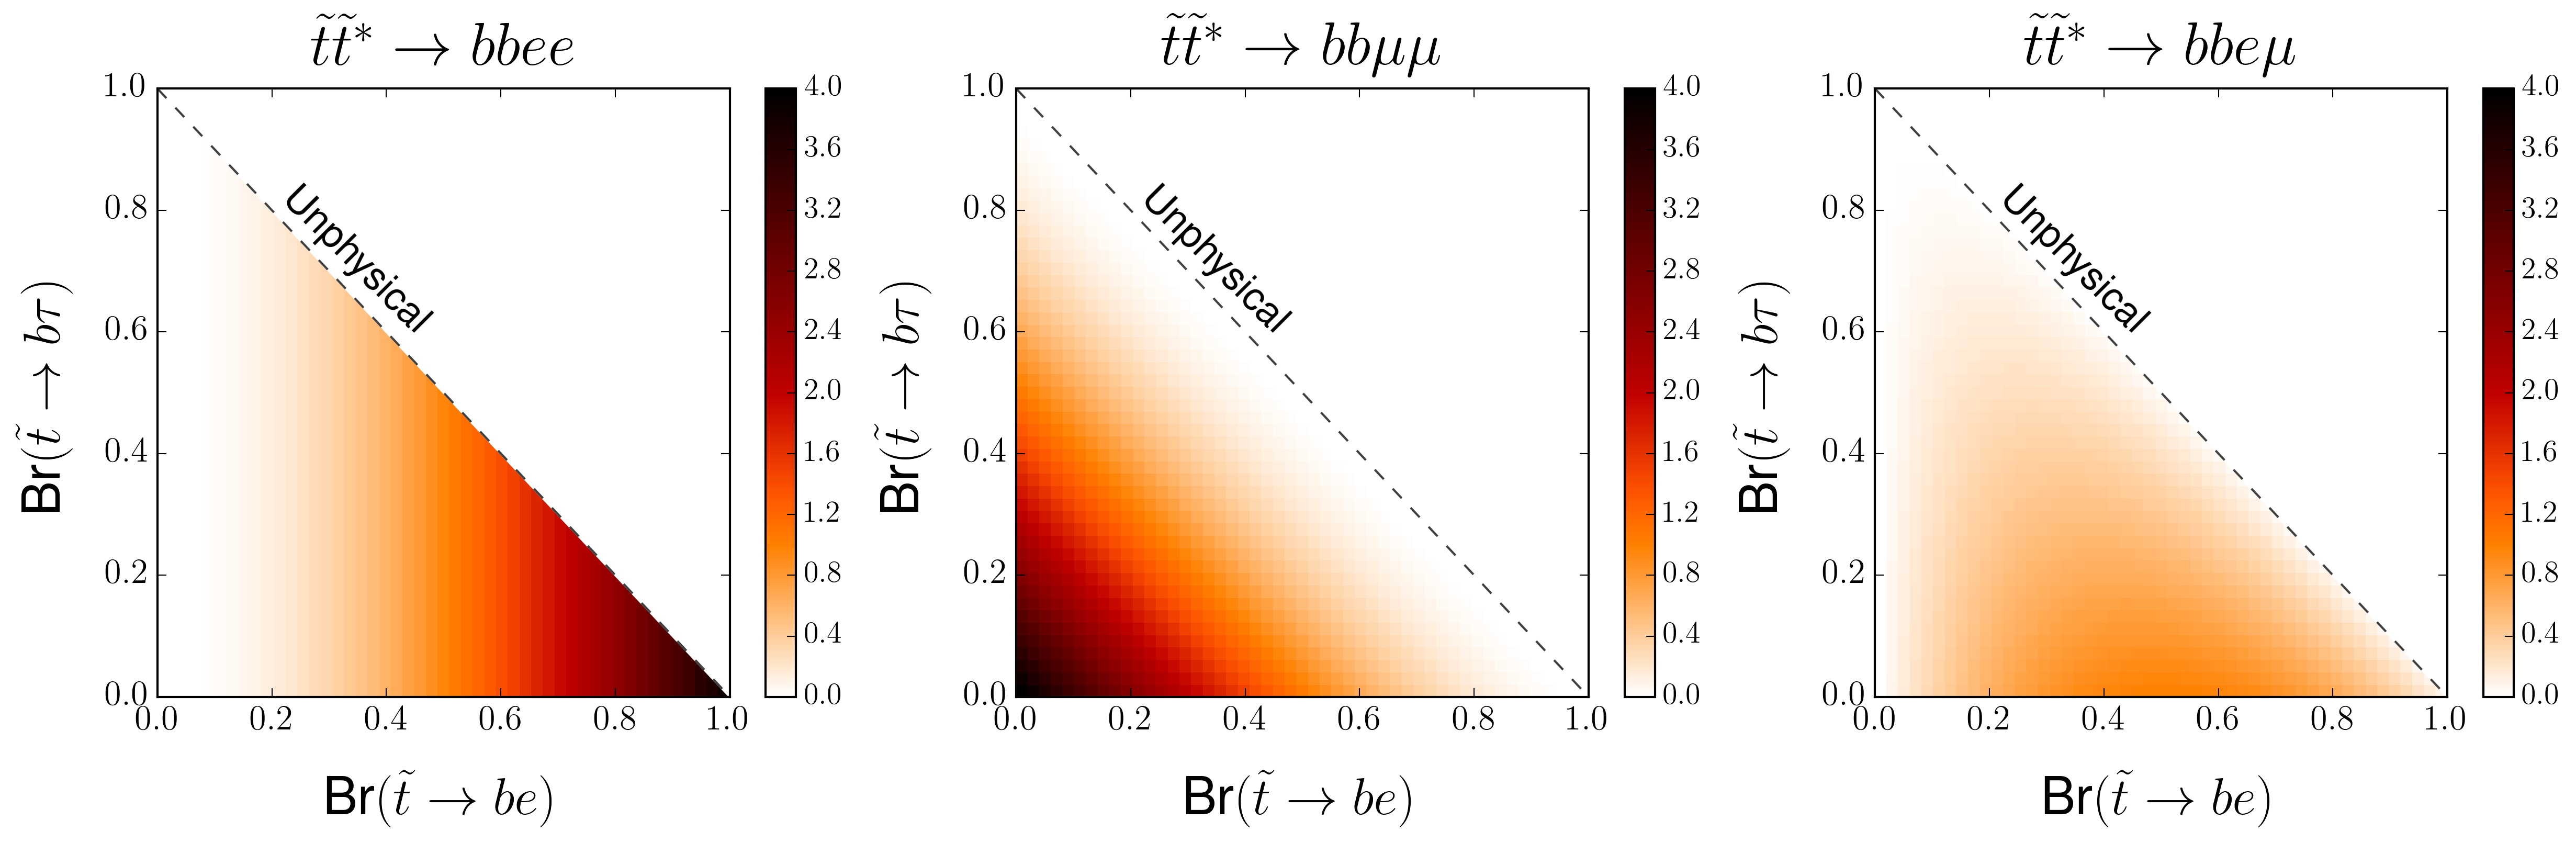
\includegraphics[width=\textwidth]{figs/blstop/scale_factors.png}
    \label{fig:flavor_scaling_sf}
  }
  \caption{Branching fraction and corresponding scale factor to each di-lepton
    flavor channel depending on the branching ratios of the stop.
    The di-stop branching fractions are given by
    Equation~\ref{eqn:branching_fractions}.
    The scale factor plot obtained by plotting
    Equation~\ref{eqn:flavor_scale_factor}.
    In all six plots, a darker color corresponds to a higher value for the
    branching fraction or the scale factor.
    {\color{red} Do I want to keep this scale factor plot in here? It's just a
      rescaling of the branching fraction plot, so it may not add anything.
    }
  }
  \label{fig:flavor_scaling}
\end{figure}

Taking the ratio of the target and nominal di-stop branching fraction, a
scale factor is defined for each flavor channel to weight the MC simulation
such that it can represent and stop branching ratio.
These scale factors are given by
\begin{equation}
  \label{eqn:flavor_scale_factor}
  \begin{aligned}
    SF_\mathrm{flavor}(\tilde{t}\tilde{t}^{*} \rightarrow bbee)     &=
      \frac{Br(\tilde{t} \rightarrow be)^2}{0.25} \\
    SF_\mathrm{flavor}(\tilde{t}\tilde{t}^{*} \rightarrow bb\mu\mu) &=
      \frac{Br(\tilde{t} \rightarrow b\mu)^2}{0.25} \\
    SF_\mathrm{flavor}(\tilde{t}\tilde{t}^{*} \rightarrow bbe\mu)   &=
      \frac{2Br(\tilde{t} \rightarrow be)Br(\tilde{t} \rightarrow b\mu)}{0.50}.
  \end{aligned}
\end{equation}
The appropriate flavor scale factor is applied to each simulated signal event
depending on the reconstructed flavor channel.
The values of the scale factors are shown in Figure~\ref{fig:flavor_scaling_sf},
where a darker corresponds to a larger value for the scale factor.

The expected and observed $CL_S$ values in SR~400 and SR~600 are shown
over a range of stop branching ratio hypotheses in
Figures~\ref{fig:cls_plane_sr_400_m_500} and~\ref{fig:cls_plane_sr_600_m_900}
respectively for select stop masses.
A complete collection of the expected and observed $CL_S$ plots are found in
Appendix~\ref{sec:axp_interpretation_plots}.

\begin{figure}[ht]
  \centering
  \subbottom[Expected $CL_S$ or SR~400]{
    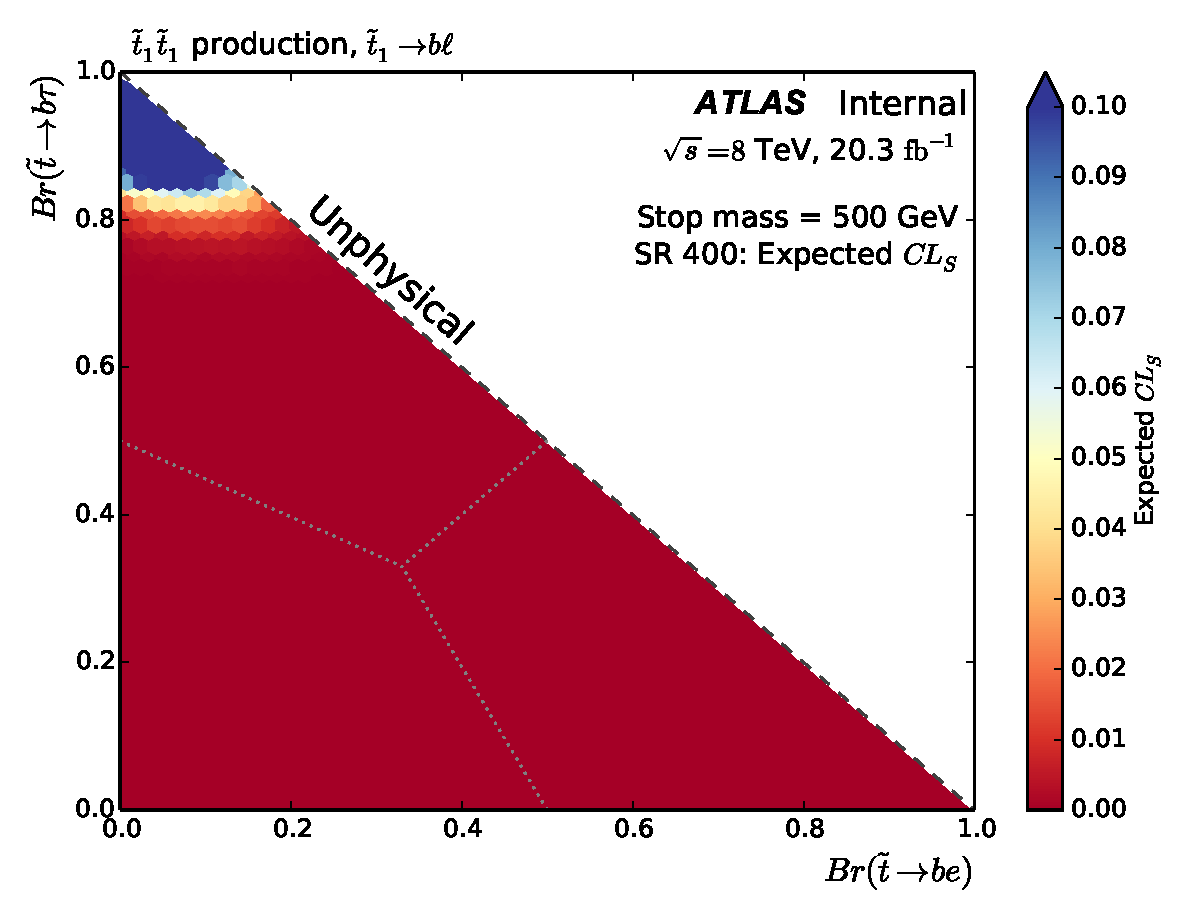
\includegraphics[width=0.48\textwidth]
      {figs/blstop/cls_plots/cls_vs_br_m_500_sr_400_exp.pdf}
  }
  \subbottom[Observed $CL_S$ or SR~400]{
    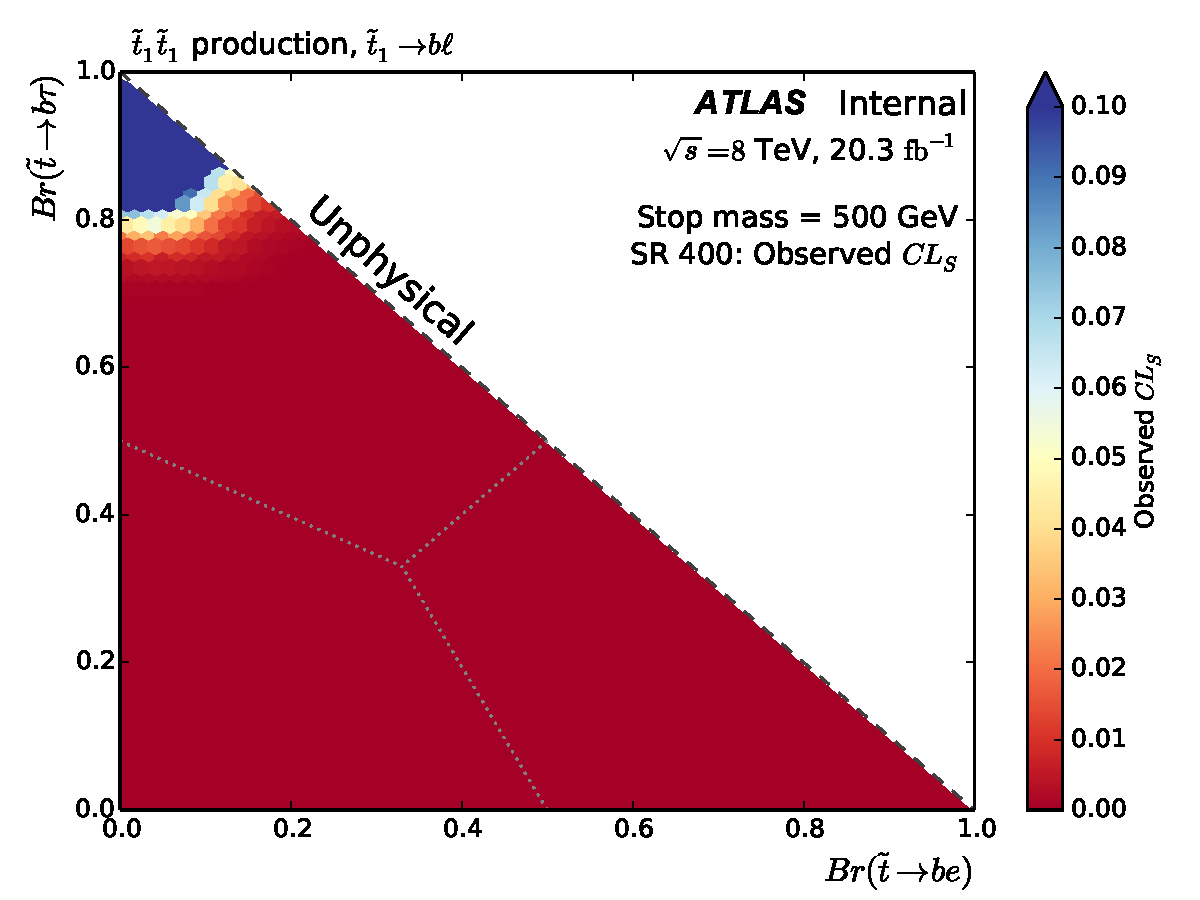
\includegraphics[width=0.48\textwidth]
      {figs/blstop/cls_plots/cls_vs_br_m_500_sr_400_obs.pdf}
  }
  \caption{
    The expected and observed $CL_S$ values in SR~400 for a stop mass of
    500~\GeV, shown across the plane of physical stop branching ratios.
  }
  \label{fig:cls_plane_sr_400_m_500}
\end{figure}

\begin{figure}[ht]
  \centering
  \subbottom[Expected $CL_S$ or SR~600]{
    \includegraphics[width=0.48\textwidth]
      {figs/blstop/cls_plots/cls_vs_br_m_900_sr_600_exp.pdf}
  }
  \subbottom[Observed $CL_S$ or SR~600]{
    \includegraphics[width=0.48\textwidth]
      {figs/blstop/cls_plots/cls_vs_br_m_900_sr_600_obs.pdf}
  }
  \caption{
    The expected and observed $CL_S$ values in SR~600 for a stop mass of
    900~\GeV, shown across the plane of physical stop branching ratios.
  }
  \label{fig:cls_plane_sr_600_m_900}
\end{figure}

A limit on the allowed stop masses and stop branching ratios is obtained
similar to the example with a single branching ratio hypothesis.
For each combination of stop mass and branching ratios, the SR which gives the
lowest expected value of $CL_S$ is selected. The SR selection for select masses
are shown in Figure~\ref{fig:sr_selection}.
Based on the selected SR, the model is rejected at 95\% CL if the observed
$CL_S$ is less than 0.05, and for each branching ratio, the highest stop mass
which is excluded is taken to be the mass limit.

\begin{figure}[ht]
  \centering
  \subbottom[Selected SR for 500~Gev stop mass]{
    \includegraphics[width=0.48\textwidth]
      {figs/blstop/region_selection/region_choice_vs_br_m_500.pdf}
  }
  \subbottom[Selected SR for 900~Gev stop mass]{
    \includegraphics[width=0.48\textwidth]
      {figs/blstop/region_selection/region_choice_vs_br_m_900.pdf}
  }
  \caption{
    The selected SR for select stop branching ratios for a stop mass of
    900~\GeV.
    The SR is selected by choosing the SR with the smallest expected $CL_S$
    value for a given branching ratio.
    For several points in the branching ratio plane, SR~400 was selected because
    the two regions have the same expected $CL_S$ value, with the numerical
    precision of the statistical software.
    For these points, the expected sensitivity for both SRs is such that
    there is little difference between the expected sensitivity.
  }
  \label{fig:sr_selection}
\end{figure}

Figure~\ref{fig:mass_limit_exp} shows the expected 95\% CL mass limit for each
point on the stop branching ratio plane.
These limits are obtained by selecting the highest stop mass with an expected
$CL_S < 0.05$ in the selected SR.
For each point on the stop branching ratio plane, the color corresponds to the
maximum excluded stop mass or the selected branching ratio hypothesis.
The nominal stop cross section is used when determining these limit contours.

\begin{figure}[ht]
  \centering
  \includegraphics[width=\textwidth]
    {figs/blstop/mass_limit_contours_no_extras_exp.pdf}
  \caption{The expected mass limit on the stop at 95\% CL.
    This limit is obtained using the nominal stop cross section.
    Stop masses between 400~\GeV\ and 1100~\GeV, in steps of 100~\GeV, are
    tested.
    The mass limit shown corresponds to the highest-mass stop sample which is
    excluded.
    {\color{red} consider moving to appendix.}
  }
  \label{fig:mass_limit_exp}
\end{figure}

The expected and observed limits for each stop mass are shown in
Figure~\ref{fig:limit_contours}.
This figure shows, for each simulated stop mass, the observed (expected)
95\% exclusion limit on the branching fraction under the red (blue) line.
A yellow band shows the $\pm 1\sigma$ uncertainty on the expected limit,
determined from the systematic uncertainty on the signal and background
prediction excluding the effect of the signal cross section uncertainty.
The effect of varying the signal cross section on the observed limit is
indicated by the dashed red lines.
Since the two observed events are in the $\mu\mu$ channel, the observed limit
is somewhat stronger than expected in scenarios with a large stop branching
fraction to $be$ (on the right side of the branching ratio plane), and somewhat
weaker than expected when the branching ratio to $b\mu$ becomes significant.
This explains why the red (observed) limit contour crosses the dashed
blue (expected) limit contour.

\begin{figure}[ht]
  \centering
  \includegraphics[width=\textwidth]{figs/blstop/limit_contours.pdf}
  \caption{Expected and observed limit on the branching ratios for the stop
    decaying to different lepton flavors shown for different stop mass
    hypotheses between 400~\GeV and 1~\TeV. The shaded area under the solid
    line represents the branching ratios which are excluded at 95\% CL
    for each stop mass.
    The dotted lines represent the uncertainty on the observed mass limit
    obtained by varying the signal model cross section up and down one standard
    deviation from the nominal value. The dashed line shows the
    expected 95\% CL exclusion for each stop mass, and the shaded band shows
    the uncertainty on this expected exclusion limit from statistical
    uncertainty and the sources of systematic uncertainty discussed in
    Section~\ref{sec:systematics}.
  }
  \label{fig:limit_contours}
\end{figure}

The observed limit on the stop mass is shown in Figure~\ref{fig:mass_limit_obs}.
This plot shows the 95\% CL on the mass obtained by choosing
the maximum excluded mass for each branching ratio on the plane using the
nominal cross section value.  
As the branching ratio of $\tilde{t} \rightarrow b\tau$ increases, the number of
expected events with electrons or muons in the final state decreases for the
same simulated stop mass.
Therefore, the limit on the mass is strongest at the bottom of the plane.
In the top corner of the plot, the SRs described in this analysis note have no
sensitivity, however traditional lepto-quark searches for final states with
$b$-tagged jets and $\tau$ leptons are able to place experimental limits in this
region \cite{ATLAS:2013oea}.

\begin{figure}[ht]
  \centering
  \includegraphics[width=\textwidth]
    {figs/blstop/mass_limit_contours_no_extras_obs.pdf}
  \caption{The observed mass limit on the stop at 95\% CL.
    This limit is obtained using the nominal stop cross section.
    Stop masses between 400~\GeV\ and 1100~\GeV, in steps of 100~\GeV, are
    tested.
    The mass limit shown corresponds to the highest-mass stop sample which is
    excluded.
  }
  \label{fig:mass_limit_obs}
\end{figure}

%% -----------------------------------------------------------------------------
\FloatBarrier
\section{Proposed improvements}
\label{sec:improvements}


%% \chapter[htoc-titlei][hhead-titlei]{htitlei}
%% -----------------------------------------------------------------------------
\chapter[Conclusion][Conclusion]{Conclusion}

This thesis describes the search for direct scalar top production where the
scalar tops decay via an $R$-parity-violating coupling to a final state with
two leptons and two identified $b$-jets.
The search uses 20.3 \ifb of $\sqrt{s}=8 \TeV$ proton-proton data collected
with the ATLAS detector at the LHC.
No significant excess of events over the Standard Model prediction is observed,
and limits are set on the mass of the scalar top at 95\% confidence level.
A scan of possible stop branching fractions are tested, the mass limit ranges
between 500~\GeV, when the stop has a branching fraction to a $b$-quark and a
tau lepton of 80\%, to to 1~\TeV when the stop decays entirely to a $b$-quark
and an electron.

With the upcoming Run-II of the Large Hadron Collider, the collisions will have
a center-of-mass energy of 13~\TeV, resulting in a huge gain in the expected
cross section for scalar top pair production.
This analysis, will benefit from the higher cross section, and will be able to
test higher stop masses.
Hopefully, the future LHC runs will find signs of new physics beyond the
Standard Model!


%%--------------------------------------------------------------------
%% appendix
%%--------------------------------------------------------------------
\appendix
%% \chapter[htoc-titlei][hhead-titlei]{htitlei}
%% -----------------------------------------------------------------------------
\chapter[Statistical interpretation technique][Statistical interpretation]
        {Statistical interpretation technique}


%% -----------------------------------------------------------------------------
\section{Likelihood function}

%% -----------------------------------------------------------------------------
\section{CLs method}


%% \chapter[htoc-titlei][hhead-titlei]{htitlei}
%% -----------------------------------------------------------------------------
\chapter[Signal model interpretation][Signal model interpretation]
        {Signal model interpretation}
\label{sec:axp_interpretation_plots}

%% -----------------------------------------------------------------------------
\begin{quote}
This appendix includes plots of the expected and observed $CL_S$ values in each
of the two SRs.
The $CL_S$ values are computed for each of the tested stop masses from 400~\GeV
to 1100~\GeV, and over the range of physical stop branching ratios.
In addition to the $CL_S$ values, the selected SR for a selection of stop
branching ratios is shown for each stop mass.
The SR is selected by choosing the SR which gives the lowest expected $CL_S$
value for the particular choice of stop mass and branching ratios as described
in Section~\ref{sec:model_dependent_limits}
\end{quote}

%% -----------------------------------------------------------------------------
\newpage
\section{400 \texorpdfstring{\GeV}{GeV} stop mass}

\begin{figure}[ht]
  \centering
  \subbottom[Expected $CL_S$ for SR~400]{
    \includegraphics[width=0.65\textwidth]
      {figs/blstop/cls_plots/cls_vs_br_m_400_sr_400_exp.pdf}
  }
  \subbottom[Expected $CL_S$ for SR~600]{
    \includegraphics[width=0.65\textwidth]
      {figs/blstop/cls_plots/cls_vs_br_m_400_sr_600_exp.pdf}
  }
  \caption{
    Expected
    $CL_S$ values for SR~400 (top) and SR~600 (bottom) for a stop mass of
    400~\GeV,
    shown across the plane of physical stop branching ratios.
  }
\end{figure}

\begin{figure}[ht]
  \centering
  \subbottom[Observed $CL_S$ for SR~400]{
    \includegraphics[width=0.65\textwidth]
      {figs/blstop/cls_plots/cls_vs_br_m_400_sr_400_obs.pdf}
  }
  \subbottom[Observed $CL_S$ for SR~600]{
    \includegraphics[width=0.65\textwidth]
      {figs/blstop/cls_plots/cls_vs_br_m_400_sr_600_obs.pdf}
  }
  \caption{
    Observed
    $CL_S$ values for SR~400 (top) and SR~600 (bottom) for a stop mass of
    400~\GeV,
    shown across the plane of physical stop branching ratios.
  }
\end{figure}

\begin{figure}[ht]
  \centering
  \includegraphics[width=0.85\textwidth]
    {figs/blstop/region_selection/region_choice_vs_br_m_400.pdf}
  \caption{
    SR selection for a stop mass of 400~\GeV.
  }
\end{figure}

\FloatBarrier

%% -----------------------------------------------------------------------------
\newpage
\section{500 \texorpdfstring{\GeV}{GeV} stop mass}

\begin{figure}[ht]
  \centering
  \subbottom[Expected $CL_S$ for SR~400]{
    \includegraphics[width=0.65\textwidth]
      {figs/blstop/cls_plots/cls_vs_br_m_500_sr_400_exp.pdf}
  }
  \subbottom[Expected $CL_S$ for SR~600]{
    \includegraphics[width=0.65\textwidth]
      {figs/blstop/cls_plots/cls_vs_br_m_500_sr_600_exp.pdf}
  }
  \caption{
    Expected
    $CL_S$ values for SR~400 (top) and SR~600 (bottom) for a stop mass of
    500~\GeV,
    shown across the plane of physical stop branching ratios.
  }
\end{figure}

\begin{figure}[ht]
  \centering
  \subbottom[Observed $CL_S$ for SR~400]{
    \includegraphics[width=0.65\textwidth]
      {figs/blstop/cls_plots/cls_vs_br_m_500_sr_400_obs.pdf}
  }
  \subbottom[Observed $CL_S$ for SR~600]{
    \includegraphics[width=0.65\textwidth]
      {figs/blstop/cls_plots/cls_vs_br_m_500_sr_600_obs.pdf}
  }
  \caption{
    Observed
    $CL_S$ values for SR~400 (top) and SR~600 (bottom) for a stop mass of
    500~\GeV,
    shown across the plane of physical stop branching ratios.
  }
\end{figure}

\begin{figure}[ht]
  \centering
  \includegraphics[width=0.85\textwidth]
    {figs/blstop/region_selection/region_choice_vs_br_m_500.pdf}
  \caption{
    SR selection for a stop mass of 500~\GeV.
  }
\end{figure}

\FloatBarrier

%% -----------------------------------------------------------------------------
\newpage
\section{600 \texorpdfstring{\GeV}{GeV} stop mass}

\begin{figure}[ht]
  \centering
  \subbottom[Expected $CL_S$ for SR~400]{
    \includegraphics[width=0.65\textwidth]
      {figs/blstop/cls_plots/cls_vs_br_m_600_sr_400_exp.pdf}
  }
  \subbottom[Expected $CL_S$ for SR~600]{
    \includegraphics[width=0.65\textwidth]
      {figs/blstop/cls_plots/cls_vs_br_m_600_sr_600_exp.pdf}
  }
  \caption{
    Expected
    $CL_S$ values for SR~400 (top) and SR~600 (bottom) for a stop mass of
    600~\GeV,
    shown across the plane of physical stop branching ratios.
  }
\end{figure}

\begin{figure}[ht]
  \centering
  \subbottom[Observed $CL_S$ for SR~400]{
    \includegraphics[width=0.65\textwidth]
      {figs/blstop/cls_plots/cls_vs_br_m_600_sr_400_obs.pdf}
  }
  \subbottom[Observed $CL_S$ for SR~600]{
    \includegraphics[width=0.65\textwidth]
      {figs/blstop/cls_plots/cls_vs_br_m_600_sr_600_obs.pdf}
  }
  \caption{
    Observed
    $CL_S$ values for SR~400 (top) and SR~600 (bottom) for a stop mass of
    600~\GeV,
    shown across the plane of physical stop branching ratios.
  }
\end{figure}

\begin{figure}[ht]
  \centering
  \includegraphics[width=0.85\textwidth]
    {figs/blstop/region_selection/region_choice_vs_br_m_600.pdf}
  \caption{
    SR selection for a stop mass of 600~\GeV.
  }
\end{figure}

\FloatBarrier

%% -----------------------------------------------------------------------------
\newpage
\section{700 \texorpdfstring{\GeV}{GeV} stop mass}

\begin{figure}[ht]
  \centering
  \subbottom[Expected $CL_S$ for SR~400]{
    \includegraphics[width=0.65\textwidth]
      {figs/blstop/cls_plots/cls_vs_br_m_700_sr_400_exp.pdf}
  }
  \subbottom[Expected $CL_S$ for SR~600]{
    \includegraphics[width=0.65\textwidth]
      {figs/blstop/cls_plots/cls_vs_br_m_700_sr_600_exp.pdf}
  }
  \caption{
    Expected
    $CL_S$ values for SR~400 (top) and SR~600 (bottom) for a stop mass of
    700~\GeV,
    shown across the plane of physical stop branching ratios.
  }
\end{figure}

\begin{figure}[ht]
  \centering
  \subbottom[Observed $CL_S$ for SR~400]{
    \includegraphics[width=0.65\textwidth]
      {figs/blstop/cls_plots/cls_vs_br_m_700_sr_400_obs.pdf}
  }
  \subbottom[Observed $CL_S$ for SR~600]{
    \includegraphics[width=0.65\textwidth]
      {figs/blstop/cls_plots/cls_vs_br_m_700_sr_600_obs.pdf}
  }
  \caption{
    Observed
    $CL_S$ values for SR~400 (top) and SR~600 (bottom) for a stop mass of
    700~\GeV,
    shown across the plane of physical stop branching ratios.
  }
\end{figure}

\begin{figure}[ht]
  \centering
  \includegraphics[width=0.85\textwidth]
    {figs/blstop/region_selection/region_choice_vs_br_m_700.pdf}
  \caption{
    SR selection for a stop mass of 700~\GeV.
  }
\end{figure}

\FloatBarrier

%% -----------------------------------------------------------------------------
\newpage
\section{800 \texorpdfstring{\GeV}{GeV} stop mass}

\begin{figure}[ht]
  \centering
  \subbottom[Expected $CL_S$ for SR~400]{
    \includegraphics[width=0.65\textwidth]
      {figs/blstop/cls_plots/cls_vs_br_m_800_sr_400_exp.pdf}
  }
  \subbottom[Expected $CL_S$ for SR~600]{
    \includegraphics[width=0.65\textwidth]
      {figs/blstop/cls_plots/cls_vs_br_m_800_sr_600_exp.pdf}
  }
  \caption{
    Expected
    $CL_S$ values for SR~400 (top) and SR~600 (bottom) for a stop mass of
    800~\GeV,
    shown across the plane of physical stop branching ratios.
  }
\end{figure}

\begin{figure}[ht]
  \centering
  \subbottom[Observed $CL_S$ for SR~400]{
    \includegraphics[width=0.65\textwidth]
      {figs/blstop/cls_plots/cls_vs_br_m_800_sr_400_obs.pdf}
  }
  \subbottom[Observed $CL_S$ for SR~600]{
    \includegraphics[width=0.65\textwidth]
      {figs/blstop/cls_plots/cls_vs_br_m_800_sr_600_obs.pdf}
  }
  \caption{
    Observed
    $CL_S$ values for SR~400 (top) and SR~600 (bottom) for a stop mass of
    800~\GeV,
    shown across the plane of physical stop branching ratios.
  }
\end{figure}

\begin{figure}[ht]
  \centering
  \includegraphics[width=0.85\textwidth]
    {figs/blstop/region_selection/region_choice_vs_br_m_800.pdf}
  \caption{
    SR selection for a stop mass of 800~\GeV.
  }
\end{figure}

\FloatBarrier

%% -----------------------------------------------------------------------------
\newpage
\section{900 \texorpdfstring{\GeV}{GeV} stop mass}

\begin{figure}[ht]
  \centering
  \subbottom[Expected $CL_S$ for SR~400]{
    \includegraphics[width=0.65\textwidth]
      {figs/blstop/cls_plots/cls_vs_br_m_900_sr_400_exp.pdf}
  }
  \subbottom[Expected $CL_S$ for SR~600]{
    \includegraphics[width=0.65\textwidth]
      {figs/blstop/cls_plots/cls_vs_br_m_900_sr_600_exp.pdf}
  }
  \caption{
    Expected
    $CL_S$ values for SR~400 (top) and SR~600 (bottom) for a stop mass of
    900~\GeV,
    shown across the plane of physical stop branching ratios.
  }
\end{figure}

\begin{figure}[ht]
  \centering
  \subbottom[Observed $CL_S$ for SR~400]{
    \includegraphics[width=0.65\textwidth]
      {figs/blstop/cls_plots/cls_vs_br_m_900_sr_400_obs.pdf}
  }
  \subbottom[Observed $CL_S$ for SR~600]{
    \includegraphics[width=0.65\textwidth]
      {figs/blstop/cls_plots/cls_vs_br_m_900_sr_600_obs.pdf}
  }
  \caption{
    Observed
    $CL_S$ values for SR~400 (top) and SR~600 (bottom) for a stop mass of
    900~\GeV,
    shown across the plane of physical stop branching ratios.
  }
\end{figure}

\begin{figure}[ht]
  \centering
  \includegraphics[width=0.85\textwidth]
    {figs/blstop/region_selection/region_choice_vs_br_m_900.pdf}
  \caption{
    SR selection for a stop mass of 900~\GeV.
  }
\end{figure}

\FloatBarrier

%% -----------------------------------------------------------------------------
\newpage
\section{1000 \texorpdfstring{\GeV}{GeV} stop mass}

\begin{figure}[ht]
  \centering
  \subbottom[Expected $CL_S$ for SR~400]{
    \includegraphics[width=0.65\textwidth]
      {figs/blstop/cls_plots/cls_vs_br_m_1000_sr_400_exp.pdf}
  }
  \subbottom[Expected $CL_S$ for SR~600]{
    \includegraphics[width=0.65\textwidth]
      {figs/blstop/cls_plots/cls_vs_br_m_1000_sr_600_exp.pdf}
  }
  \caption{
    Expected
    $CL_S$ values for SR~400 (top) and SR~600 (bottom) for a stop mass of
    1~\TeV,
    shown across the plane of physical stop branching ratios.
  }
\end{figure}

\begin{figure}[ht]
  \centering
  \subbottom[Observed $CL_S$ for SR~400]{
    \includegraphics[width=0.65\textwidth]
      {figs/blstop/cls_plots/cls_vs_br_m_1000_sr_400_obs.pdf}
  }
  \subbottom[Observed $CL_S$ for SR~600]{
    \includegraphics[width=0.65\textwidth]
      {figs/blstop/cls_plots/cls_vs_br_m_1000_sr_600_obs.pdf}
  }
  \caption{
    Observed
    $CL_S$ values for SR~400 (top) and SR~600 (bottom) for a stop mass of
    1~\TeV,
    shown across the plane of physical stop branching ratios.
  }
\end{figure}

\begin{figure}[ht]
  \centering
  \includegraphics[width=0.85\textwidth]
    {figs/blstop/region_selection/region_choice_vs_br_m_1000.pdf}
  \caption{
    SR selection for a stop mass of 1~\TeV.
  }
\end{figure}

\FloatBarrier

%% -----------------------------------------------------------------------------
\newpage
\section{1100 \texorpdfstring{\GeV}{GeV} stop mass}

\begin{figure}[ht]
  \centering
  \subbottom[Expected $CL_S$ for SR~400]{
    \includegraphics[width=0.65\textwidth]
      {figs/blstop/cls_plots/cls_vs_br_m_1100_sr_400_exp.pdf}
  }
  \subbottom[Expected $CL_S$ for SR~600]{
    \includegraphics[width=0.65\textwidth]
      {figs/blstop/cls_plots/cls_vs_br_m_1100_sr_600_exp.pdf}
  }
  \caption{
    Expected
    $CL_S$ values for SR~400 (top) and SR~600 (bottom) for a stop mass of
    1.1~\TeV,
    shown across the plane of physical stop branching ratios.
  }
\end{figure}

\begin{figure}[ht]
  \centering
  \subbottom[Observed $CL_S$ for SR~400]{
    \includegraphics[width=0.65\textwidth]
      {figs/blstop/cls_plots/cls_vs_br_m_1100_sr_400_obs.pdf}
  }
  \subbottom[Observed $CL_S$ for SR~600]{
    \includegraphics[width=0.65\textwidth]
      {figs/blstop/cls_plots/cls_vs_br_m_1100_sr_600_obs.pdf}
  }
  \caption{
    Observed
    $CL_S$ values for SR~400 (top) and SR~600 (bottom) for a stop mass of
    1.1~\TeV,
    shown across the plane of physical stop branching ratios.
  }
\end{figure}

\begin{figure}[ht]
  \centering
  \includegraphics[width=0.85\textwidth]
    {figs/blstop/region_selection/region_choice_vs_br_m_1100.pdf}
  \caption{
    SR selection for a stop mass of 1.1~\TeV.
  }
\end{figure}

\FloatBarrier

%% \begin{figure}[ht]
%%   \centering
%%   \subbottom[Expected $CL_S$ for SR 400]{
%%     \includegraphics[width=0.48\textwidth]
%%       {figs/blstop/cls_plots/cls_vs_br_m_400_sr_400_exp.pdf}}
%%   \subbottom[Expected $CL_S$ for SR 600]{
%%     \includegraphics[width=0.48\textwidth]
%%       {figs/blstop/cls_plots/cls_vs_br_m_400_sr_600_exp.pdf}}
%%   % \subbottom[Selected region]{
%%   %   \includegraphics[width=0.48\textwidth]
%%   %     {figs/blstop/region_selection/region_choice_vs_br_m_400.pdf}}
%%   \caption{blah blah blah expected blah blah blah}
%% \end{figure}

% \begin{figure}[ht]
%   \centering
%   \subbottom[Observed $CL_S$ for SR 400]{
%     \includegraphics[width=0.40\textwidth]
%       {figs/blstop/cls_plots/cls_vs_br_m_400_sr_400_obs.pdf}}
%   \subbottom[Observed $CL_S$ for SR 600]{
%     \includegraphics[width=0.40\textwidth]
%       {figs/blstop/cls_plots/cls_vs_br_m_400_sr_600_obs.pdf}}
%   \caption{blah blah blah observed blah blah blah}
% \end{figure}

% \FloatBarrier


%% figs/blstop/cls_plots/cls_vs_br_m_500_sr_400_exp.pdf
%% figs/blstop/cls_plots/cls_vs_br_m_500_sr_400_obs.pdf
%% figs/blstop/cls_plots/cls_vs_br_m_500_sr_600_exp.pdf
%% figs/blstop/cls_plots/cls_vs_br_m_500_sr_600_obs.pdf
%% figs/blstop/cls_plots/cls_vs_br_m_600_sr_400_exp.pdf
%% figs/blstop/cls_plots/cls_vs_br_m_600_sr_400_obs.pdf
%% figs/blstop/cls_plots/cls_vs_br_m_600_sr_600_exp.pdf
%% figs/blstop/cls_plots/cls_vs_br_m_600_sr_600_obs.pdf
%% figs/blstop/cls_plots/cls_vs_br_m_700_sr_400_exp.pdf
%% figs/blstop/cls_plots/cls_vs_br_m_700_sr_400_obs.pdf
%% figs/blstop/cls_plots/cls_vs_br_m_700_sr_600_exp.pdf
%% figs/blstop/cls_plots/cls_vs_br_m_700_sr_600_obs.pdf
%% figs/blstop/cls_plots/cls_vs_br_m_800_sr_400_exp.pdf
%% figs/blstop/cls_plots/cls_vs_br_m_800_sr_400_obs.pdf
%% figs/blstop/cls_plots/cls_vs_br_m_800_sr_600_exp.pdf
%% figs/blstop/cls_plots/cls_vs_br_m_800_sr_600_obs.pdf
%% figs/blstop/cls_plots/cls_vs_br_m_900_sr_400_exp.pdf
%% figs/blstop/cls_plots/cls_vs_br_m_900_sr_400_obs.pdf
%% figs/blstop/cls_plots/cls_vs_br_m_900_sr_600_exp.pdf
%% figs/blstop/cls_plots/cls_vs_br_m_900_sr_600_obs.pdf
%% 
%% figs/blstop/cls_plots/cls_vs_br_m_1000_sr_400_exp.pdf
%% figs/blstop/cls_plots/cls_vs_br_m_1000_sr_400_obs.pdf
%% figs/blstop/cls_plots/cls_vs_br_m_1000_sr_600_exp.pdf
%% figs/blstop/cls_plots/cls_vs_br_m_1000_sr_600_obs.pdf
%% figs/blstop/cls_plots/cls_vs_br_m_1100_sr_400_exp.pdf
%% figs/blstop/cls_plots/cls_vs_br_m_1100_sr_400_obs.pdf
%% figs/blstop/cls_plots/cls_vs_br_m_1100_sr_600_exp.pdf
%% figs/blstop/cls_plots/cls_vs_br_m_1100_sr_600_obs.pdf
%% 
%% figs/blstop/region_selection/region_choice_vs_br_m_500.pdf
%% figs/blstop/region_selection/region_choice_vs_br_m_600.pdf
%% figs/blstop/region_selection/region_choice_vs_br_m_700.pdf
%% figs/blstop/region_selection/region_choice_vs_br_m_800.pdf
%% figs/blstop/region_selection/region_choice_vs_br_m_900.pdf
%% figs/blstop/region_selection/region_choice_vs_br_m_1000.pdf
%% figs/blstop/region_selection/region_choice_vs_br_m_1100.pdf

\end{Spacing}

%%--------------------------------------------------------------------
%% bibliography
%%--------------------------------------------------------------------
\backmatter
\bibliographystyle{style/atlasnote}
\bibliography{bibs/atlas,bibs/atlas_egamma,bibs/atlas_jets,bibs/atlas_lumi,bibs/atlas_met,bibs/atlas_muons,bibs/jets,bibs/leptoquark,bibs/mc_generators,bibs/single_top,bibs/susy,bibs/susy_bl,bibs/susy_cross_section,bibs/susy_light_stop_mass,bibs/susy_rpc,bibs/susy_signatures,bibs/susy_top_down,bibs/ttbar,bibs/statistics,bibs/lhc,bibs/sm,bibs/atlas_sm,bibs/atlas_quality}

%%--------------------------------------------------------------------
\end{document}

